%! program = pdflatex

\documentclass[twoside,onecolumn,11pt,a4paper,final]{book}
\usepackage[activate={true,nocompatibility},final]{microtype}
\usepackage[utf8]{inputenc}

\pdfminorversion=5
\pdfobjcompresslevel=2

%\usepackage{cite} % sort multiple citations alphanumerically
\usepackage[numbers,sort&compress]{natbib}
%\usepackage{natbib}
%\bibliographystyle{unsrt} 
%\bibliographystyle{agsm}
%\bibliographystyle{unsrtnat}
\bibliographystyle{apsrev}

%\usepackage[utf8x]{inputenc} % Any characters can be typed directly from the keyboard, eg éçñ
%\usepackage[russian,australian]{babel}
%\usepackage[russian]{babel}
\usepackage{anuthesis}
%\usepackage{fancyhdr}

\usepackage[dvipsnames,usenames]{xcolor}
\usepackage[final]{graphicx}
\usepackage{rotating}

\usepackage{amsmath}
\usepackage{amssymb}
\usepackage{amsfonts}
\usepackage[T1,OT2,OT1]{fontenc}
\usepackage{gensymb}
\usepackage{esint}
\usepackage{slashed}

%\usepackage{flafter}  % Don't place floats before their definition
%\usepackage{unicode}

\usepackage{textcomp} % provide lots of new symbols
\usepackage{bm}  % Define \bm{} to use bold math fonts
%\usepackage{setspace} % Useful for doublespacing for drafts
\usepackage{relsize}


%%% PACKAGES
\usepackage{booktabs} % for much better looking tables
%\usepackage{array} % for better arrays (eg matrices) in maths
\usepackage{paralist} % very flexible & customisable lists (eg. enumerate/itemize, etc.)
\usepackage{verbatim} % adds environment for commenting out blocks of text & for better verbatim
\usepackage{units}
\usepackage{enumerate}

%%% SECTION TITLE APPEARANCE
\usepackage{sectsty}
\allsectionsfont{\fontfamily{dop}\sffamily\selectfont}

%%% ToC APPEARANCE
\usepackage[nottoc,notlof,notlot]{tocbibind} % Put the bibliography in the ToC
%\usepackage[titles]{tocloft} % Alter the style of the Table of Contents
%\renewcommand{\cftsecfont}{\rmfamily\mdseries\upshape}
%\renewcommand{\cftsecpagefont}{\rmfamily\mdseries\upshape} % No bold!

%\usepackage[draft]{showkeys} % show references in draft format
\usepackage{ifthen}


%\usepackage{notoccite}
\usepackage{url}
\usepackage[pdftex, bookmarks, colorlinks, breaklinks, pdfauthor=Graham\ Russell\ Dennis, pdftitle=Pumping\ an\ atom\ laser, final]{hyperref}  % PDF hyperlinks, with coloured links
\definecolor{dullmagenta}{rgb}{0.4,0,0.4}   % #  660066
\definecolor{darkblue}{rgb}{0,0,0.4}
%\hypersetup{linkcolor=red,citecolor=blue,filecolor=dullmagenta,urlcolor=darkblue} % coloured links
\hypersetup{linkcolor=black,citecolor=black,filecolor=black,urlcolor=black} % black links, for printed output
%\usepackage{hypernat}
% \usepackage{fancybox}
% \fancyput(5cm ,1 cm)
%   {
%       \textcolor{lightgray}{DRAFT: \today}
%   }

\usepackage{typedref}
%\refname{section}{}{S}

\renewcommand{\bottomfraction}{0.7}  

\newcommand{\divg}{\ensuremath{\nabla\cdot}}
\newcommand{\curl}{\ensuremath{\nabla\times}}
\newcommand{\grad}{\ensuremath{\nabla}}

\newcommand{\ket}[1]{{\ensuremath{\left|#1\right>}}}
\newcommand{\mean}[1]{{\ensuremath{\big<#1\big>}}}
\newcommand{\bra}[1]{\ensuremath{\left<#1\right|}}
\newcommand{\braket}[2]{\ensuremath{\left<#1\middle|#2\right>}}
\newcommand{\ketbra}[2]{\ensuremath{\left|#1\middle>\!\middle<#2\right|}}
\newcommand{\abs}[1]{\ensuremath{\left|#1\right|}}
\newcommand{\comm}[1]{\ensuremath{\big[#1\big]}}

\DeclareMathOperator{\Tr}{Tr}
\DeclareMathOperator{\sech}{sech}
\renewcommand{\Re}{\operatorname{Re}}
\renewcommand{\Im}{\operatorname{Im}}

\newcommand{\pislash}{\slashed{\pi}}

\newcommand\relphantom[1]{\mathrel{\phantom{#1}}}

\newcommand\vect[1]{\ensuremath{\bm{#1}}}
\newcommand\unitvec[1]{\ensuremath{\check{\vect{#1}}}}

\newcommand{\nucl}[2]{\ensuremath{^{#1}\text{#2}}}

\newcommand{\parasep}{\begin{center} 
\includegraphics[scale=0.8]{HRule} \end{center}}
\newcommand{\Kunpol}{\ensuremath{K^\text{(unpol)}_{^4\text{He}}}}
%\allowdisplaybreaks[1]

\newcommand{\xpdeint}{\texttt{xpdeint}}
\newcommand{\XMDS}{\texttt{XMDS}}

\begin{document}

\pagenumbering{roman}  % first use Roman numerals for page numbers

\begin{titlepage}
\graphicspath{{Figures/TitlePage/}{Figures/Common/}}
\title{\textbf{\relsize{2} Pumping an atom laser}\\[2cm]}
 \author{Graham Russell Dennis\\[6cm]
 
\includegraphics{ANU_PMS}\\[2cm]
  A thesis submitted for the degree of\\
  Doctor of Philosophy\\
  at The Australian National University\\[1cm]}
%  \date{\today}
\maketitle
\end{titlepage}

\sloppy

\thispagestyle{empty}
\newenvironment{dedication}
  {\cleardoublepage \thispagestyle{empty} \vspace*{\stretch{1}} \begin{flushright} \em}
  {\end{flushright} \vspace*{\stretch{3}} \clearpage}
\begin{dedication}
In memory of those we have lost these past few months:\\ Nikki, Elva \& Scotchie.
\end{dedication}


\chapter*{Declaration}
%\addcontentsline{toc}{chapter}{Declaration}

% This thesis is an account of research undertaken under the supervision of Dr.\ Joseph Hope between February 2006 and May 2010 at The Department of Quantum Science, Research School of Physical Sciences and Engineering, The Australian National University, Canberra, Australia.
% 
Except where acknowledged in the customary manner, the material 
presented in this thesis is, to the best of my knowledge, original and 
has not been submitted in whole or part for a degree in any 
university.

\vspace{20mm}  % vertical space

\hspace{80mm}\rule{40mm}{.15mm}\par   % horizontal space, line, start new line
\hspace{80mm} Graham Russell Dennis\par
\hspace{80mm} May 2010


% include statements effectively insert the contents of the named file.
% They are not necessary, but are useful for organising your work.
% They always start a  new page.

\chapter*{Acknowledgements}
\graphicspath{{Figures/Common/}}

% People to thank:
% Supervisor/s: Joe Hope, Craig Savage, John Close.
% Family
% Friends
% Colleagues / coworkers: Julien Dugué, Oliver Topic, Justin Schultz, Simon Haine, Mattias Johnsson, Matthew Jeppesen, Sven Abend, André de Carvalho, Paul Altin, John Debs, Rachel Poldy, Ben Buchler, Stuart Szigeti, Robin Stevenson, Michael Hush, Daniel Döring, Gordon McDonald, Finn Lattimore, Kate Wagner, Jean-François Morizur, Mahdi Housseni, Nick Robins, Cristina Figl, Paul Summers

% Olympiad people for keeping me sane.  Mainly Kate, Matt & Alix. & Lucy

% An institution that will remain nameless for demonstrating the meaning of incompetence.

% Dave Singleton for not yelling at me too much when I managed to crash a supercomputer.

% People I have collaborated with with: Matt Davis, Andrew Truscott, Rob Dall

%I'd like to thank John for the endless games of hide-and-seek played in the last week.

% Proof-readers: John, Joe, Cristina, Mattias, Stuart, Robin, Michael, Rob.

% I would like to thank my lucky stars, and the cat, for not eating me.

First and foremost, I would like to thank my supervisors: Joe, John and Craig.  I have learnt much these past few years, and that could not have happened without your guidance.  

My supervisors have been invaluable in the writing of this thesis, as have my other proof-readers: André, Cristina, Daniel, Mattias, Michael, Rob, Robin, and Stuart.

I have had many interesting and enlightening discussions with people too numerous to count, but I must particularly thank Nick for his endless patience explaining the goings on of experimental physics, and Mattias \& Simon for teaching me the tricks with performing numerical simulations.

Over the past several years, I have had the great pleasure to work with an incredible group of people in the Physics Olympiad program.  In particular, I would like to thank Kate, Matt, Alix \& Lucy.  Who could ever thought it was possible to have fun while writing an exam?  As strange as it sounds, you have helped keep me sane.

Throughout my PhD, I have collaborated closely with the Rubidium and Helium BEC experimental groups at the ANU.  In particular, I would like to thank John, Nick \& Cristina from the Rubidium group and Andrew \& Rob from the Helium group for helping me learn the `language' of experimental physics.

I would like to thank the many people with whom I have shared my time at the `department of many names': André, Ben, Cristina, Daniel, Emily, Finn, Gordon, JD, Jean-François, Julien, Justin, Kate, Mahdi, Matthew, Mattias, Michael, Nick, Oliver, Paul~A., Paul~S., Rachel, Robin, Simon, Stuart, Sven and Tom.  You have been excellent company.  In time, perhaps, I can repay my debt of baked goods and chocolate.

Finally, I would like to thank my parents Greg \& Lynda.  You have encouraged me to delve into the nature of things, and to seek the satisfaction of understanding.

\chapter*{Abstract}
%\addcontentsline{toc}{chapter}{Abstract}
\graphicspath{{Figures/Common/}}


Measurement is our fundamental tool for learning about the world around us.  It is from observing trends in measurements that we develop the theories that enable us to predict future behaviour, and it is against measurements that we determine the validity of these theories.  Increases in the precision of our measurements are fundamental to our understanding.

Atom interferometry is a new method for performing precision measurements that uses the matter-wave nature of atoms to perform interferometry experiments analogous to those performed with photons.  However, in contrast to optical interferometry, which uses coherent sources of photons, atom interferometry uses thermal atomic sources, in part due to the unavailability of high-flux coherent atomic sources.  Although pulsed coherent atomic sources are presently available, continuous sources are not.  Creating a truly continuous coherent source for atoms is tricker than for photons.  One of the largest challenges is that atom number is conserved.  A source of atoms is therefore necessary to produce a truly continuous atom laser.  This source must be used to replenish the lasing mode of the atom laser, and the process must operate without significantly disturbing the coherence properties of the lasing mode.  It is this replenishment or pumping process that has been investigated theoretically in this thesis.

There are only two choices for the reservoir that makes the replenishment (or pumping) process of an atom laser irreversible: the empty modes of the optical field, and the empty modes of the atomic field.  Processes of both forms are considered.  Using an optical reservoir has the advantage that atoms are not necessarily lost as part of the pumping process, which is necessary when using an atomic reservoir.  The efficiency of processes using an optical reservoir can therefore be higher.  Using an atomic reservoir, however, has the advantage that it is experimentally easier to implement as one can use the standard experimental technique of evaporation which is commonly used in the production of pulsed coherent atomic sources.  We show theoretically in this thesis that although it is possible to produce a continuous atom laser using an atomic reservoir, the flux achieved in the geometry considered is insufficient to compete with pulsed coherent atomic sources for precision measurement.  The results for the pumping process using an optical reservoir are more promising.  Although condensed sources were used as the source for this process, a detailed comparison of the theoretical calculations and experimental results indicate that the detrimental reabsorption processes are suppressed.  This suggests that it may be possible to use higher-flux thermal atomic sources to replenish the lasing mode of an atom laser with this pumping process.

\tableofcontents
%\listoffigures % makes a list of figures
%\listoftables  % uncomment this if you have tables
\cleardoublepage

\pagenumbering{arabic} % switch to Arabic numerals for page numbers
\setcounter{page}{1}  % set page number to 1

\chapter{Introduction}
\label{Introduction}
\graphicspath{{Figures/Introduction/}{Figures/Common/}}

It is hard to underestimate the effect that the laser has had since its invention in 1960 \citep{Maiman:1960}.  Although initially motivated by pure scientific curiosity, its unique properties have given it application in an astonishing array of technologies, in addition to its use as a powerful tool in fundamental research.  

Laser radiation is distinguished from the light emitted by everyday light sources --- such as light bulbs --- by three main properties, (i) its narrow divergence, (ii) the narrow range of frequencies that are emitted, and (iii) the low intensity noise of the emitted radiation.  Although many applications only make use of the first property, the second property is critical to its use in such applications as laser gyroscopes, gravitational wave detection and fundamental tests of quantum mechanics\footnote{FIXME: Add citations}.  This second property can also be achieved for thermal light through appropriate spectral filtering, however in practice, lasers are a more convenient method for achieving high spectral intensities.  The third property is the true distinguishing property of a laser, however it is only important in specialised applications (e.g.\ gravitational wave detection), in which intensity fluctuations are a significant noise source\footnote{FIXME: In what other circumstances is $g^{(2)}$ important?}.

Quantum mechanics tells us that not only can light behave as a wave, but atoms can too.  This wave nature of atoms is usually indiscernible because the typical wavelength for a thermal atom is many orders of magnitude smaller than the inter-atomic spacing ($\lambda \sim 5 \times\unit[10^{-11}]{m}$ as compared to $d \sim 3 \times\unit[10^{-9}]{m}$).  However, in 1925 Einstein predicted \citep{Einstein:1925} that if a gas of \emph{bosons} (a class of particles which includes many atomic species) was cooled below a critical temperature, a large fraction of the particles would occupy the ground state of the system, forming a coherent wavefunction.  This was achieved in 1995 for dilute atomic gases \citep{Anderson:1995vn,Bradley:1995ys,Davis:1995} with the first production of a Bose-Einstein Condensate (BEC), a macroscopic occupation of atoms in a single spatial mode.  As it is the macroscopic occupation of \emph{photons} in a single spatial mode that gives the optical laser many of its properties, with the achievement of BEC it has become possible to consider the creation of an atomic analogue of the optical laser: the \emph{atom} laser.

An atom laser, while ideally sharing the above properties of its optical cousin, would behave very differently to an optical laser.  While photons interact strongly with matter, they interact only weakly with themselves or with gravity.  While this makes lasers robust to fluctuations in electromagnetic or gravitational fields, they are therefore less sensitive to these fields in interferometry experiments.  Despite this limitation, optical interferometry has been used in several incredible gravitational experiments, including GRACE, LIGO, and Gravity Probe-A \citep{Vessot:1980}.

As atoms interact more readily with their environment than photons, atom interferometry has a broad range of applications: to the measurement of electric and magnetic fields in tests of atom and neutron charge neutrality \citep{Arvanitaki:2008}, an application which would be essentially impossible with optical lasers due to the weak photon--photon interaction; to fundamental tests of predictions of General Relativity \citep{Dimopoulos:2007uq}; to the development of gyroscopes \citep{Gustavson:1997}, gradiometers \citep{Snadden:1998,McGuirk:2002} and gravimeters \citep{Peters:2001}, which, while possible using optical lasers, their atomic counterparts are far more compact due to the significantly stronger gravitational interaction.

Discussion of cold thermal atom interferometry, and how this can be improved through the use of atom lasers.  In particular, space-based applications where the interrogation time is larger \citep{Le-Coq:2006}, therefore we need a greater control over the velocity distribution, and therefore $g^{(1)}$.

Rotation sensing using cold thermal atom clouds: \citep{Canuel:2006}, measuring Newton's constant $G$: \citep{Lamporesi:2008}

FIXME: The basic plan for this section: lasers are cool, now that we have BEC, wouldn't it be cool to have an atom laser.  Optical lasers have great application to interferometry, atoms behave differently and have advantages and disadvantages for interferometry applications.  In certain circumstances, we will need atom-laser based matter-wave interferometry, not just thermal atom interferometry.  Fundamentally, this is about the degree of control.  In the far future, if we want entangled matter-wave sources, we have better prospects using a condensed source like an atom laser.

\section{Photon lasers and Atom lasers}
\label{Introduction:PhotonAndAtomLasers}

The basic features necessary of a continuous atom laser are analogous to the features of a continuous photon laser: a resonant, a lasing mode, an outcoupling process, and a Bose-stimulated pumping mechanism (see \figureref{Introduction:LaserAtomLaserComparison}).  The first three of these features are well understood for an atom laser; experimentally realising the fourth, the pumping mechanism, has presented the greatest challenge.

\begin{figure}
    \centering
    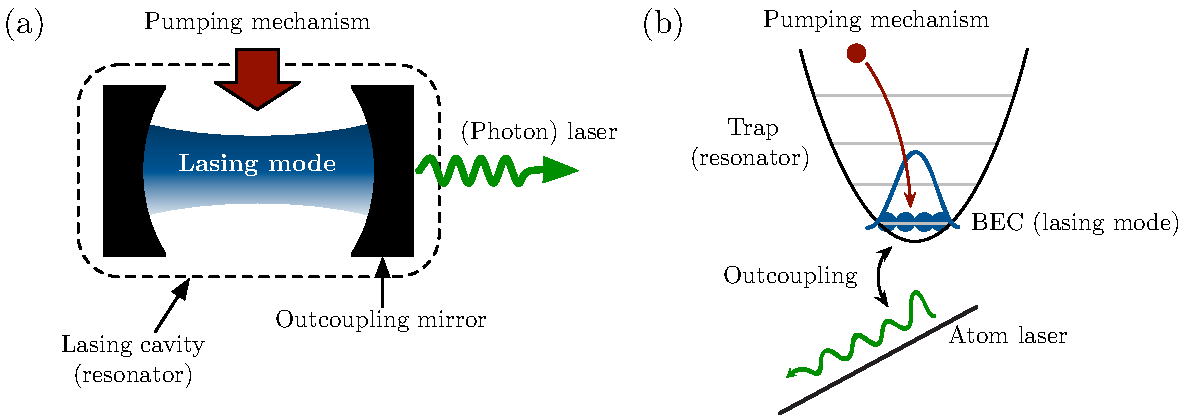
\includegraphics[width=14cm]{LaserAtomLaserComparison}
    \caption{
        \label{Introduction:LaserAtomLaserComparison}
        FIXME: This is not a caption.
    }
\end{figure}

\subsection{The resonator}

In a photon laser, the resonator is typically a cavity formed between two (or more) mirrors trapping the photons with a region of space; the optical mode trapped within the resonator is the lasing mode.  For atom laser, the resonator is an `atom trap', either an optical trap using the ac Stark shift to trap the atoms in a region of high optical intensity, or a magnetic trap using the Zeeman shift to selectively trap certain magnetic hyperfine states near a local minimum of the magnetic field.

\subsection{The lasing mode}

\begin{figure}
    \centering
    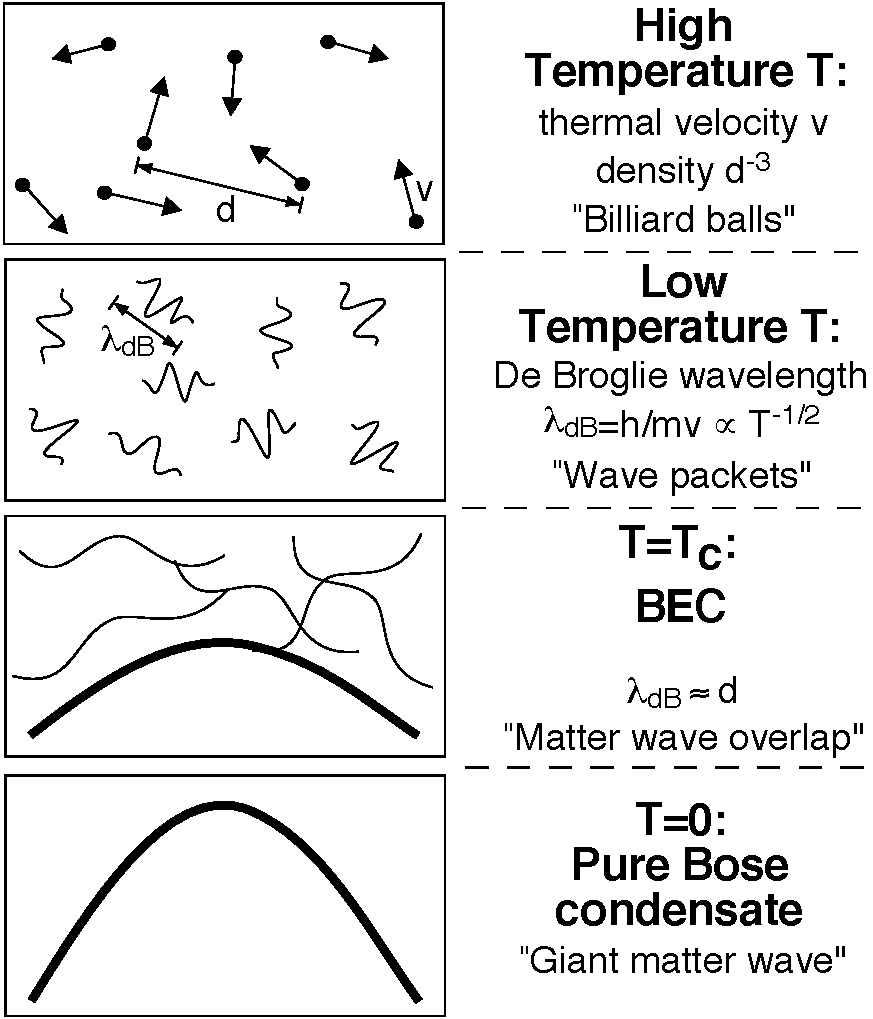
\includegraphics[width=8cm]{WhatIsBEC}
    \caption{
        \label{Introduction:WhatIsBEC}
        FIXME: This is not a caption.  Figure stolen without permission from \citep{Ketterle:1999fk}.
    }
\end{figure}

The necessary property for the lasing mode of a laser --- be it optical or atomic --- is that it have an occupation much greater than one \citep{Wiseman:1997ba}.  For photons, such a highly-degenerate mode was first achieved with the development of the photon laser itself \citep{Maiman:1960,Javan:1961}; a photon condensate cannot exist in equilibrium as total photon number is not conserved \citep{Muller:1986,Ketterle:1999fk}.  Total atom number is, however, conserved and Bose-Einstein condensation occurs below a critical temperature \citep{PethickSmith}.  Below this critical temperature, a significant fraction of the atoms in the system occupy a single spatial mode; exactly what is required of the lasing mode of an atom laser.

The process of Bose-Einstein condensation can be understood in a simplified picture in which the atoms are viewed as wave-packets with an extent of the order of the thermal de Broglie wavelength $\lambda_\text{dB} = (2 \pi \hbar^2 / M k_B T)^{1/2}$, where $M$ is the mass of the atom, $k_B$ is Boltzmann's constant, and $T$ is the temperature of the atoms.  At room temperature, the de Broglie wavelength is sufficiently small ($\sim 5\times\unit[10^{-11}]{m}$ for \nucl{4}{He} at $T=\unit[300]{K}$) that the atoms behave as point-like billiard balls (upper panel of \figureref{Introduction:WhatIsBEC}).  As the temperature decreases, the de Broglie wavelength increases (second panel of \figureref{Introduction:WhatIsBEC}).  As the temperature continues to decrease, the de Broglie wavelength approaches the mean interparticle separation $d$ and the atomic matter waves begin to overlap (third panel of \figureref{Introduction:WhatIsBEC}).  Below this temperature, a Bose-Einstein condensate begins to form, until at $T=0$, all atoms are in the condensate (lower panel of \figureref{Introduction:WhatIsBEC}).  Conservation of total number is necessary for BEC, as it is because of this that the interparticle separation $d$ remains constant as temperature is decreased (in a box of constant volume); for photons, as the temperature is decreased the total number of photons in the system decreases, increasing the mean interparticle separation $d$ faster than the photon wavelength increases.  Hence photon condensation cannot occur in equilibrium.

Bose-Einstein condensation is a macroscopic quantum phenomenon with a broad range of applications beyond the production of atom lasers.  Perhaps the most interesting of these are the development of \emph{quantum simulators} \citep{Lewenstein:2007,Buluta:2009}, experiments which directly realise theoretical condensed matter models, which where initially proposed as approximations to other systems.  For example, the Bose-Hubbard model \citep{Fisher:1989} of interacting bosons was realised by loading a BEC into an optical lattice.  By changing the depth of the optical lattice, the ratio of the tunnelling and interaction terms was be changed, permitting direct observation of the superfluid--Mott insulator transition \citep{Greiner:2002lr}.  Quantum simulators are possible for a variety of other systems, including Josephson junctions \citep{Levy:2007vn}, and reduced-dimensional systems such as the Tonks-Girardeau model of 1D hard core bosons \citep{Girardeau:1960,Lieb:1963,Paredes:2004}.  Dilute gas BECs have also been used in the direct observation of persistent currents in the form of vortices and vortex lattices \citep{Abo-Shaeer:2001}, the coherent control of optical information \citep{Ginsberg:2007fk}, and the observation of quantum optical effects in atoms such as the Hanbury-Brown-Twiss effect \citep{Jeltes:2007fk}, and four-wave mixing \citep{Deng:1999qy}.

% Theoretical things not included in the above list:
% realisation of an analogue to a magnetic monopole \citep{Pietila:2009}
% super-chemistry \citep{Heinzen:2000}: perform a chemical reaction in a controlled way, from a desired initial state to a desired final quantum state
% GR-analogues

% Other things not mentioned:
% Testing Bogoliubov's theory for excitations and the speed of sound (temperature dependence too)

One of the advantages of dilute gas BEC that gives these systems such a broad range of applications is the extraordinary degree to which these systems can be controlled and manipulated:  their effective dimensionality can be changed by changing the confining potential; the de Broglie wavelength is controllable over many orders of magnitude $\unit[1]{nm} \lesssim \lambda_\text{dB} \lesssim \unit[10]{\micro m}$; the sign and magnitude of interparticle interactions can be controlled \citep{Inouye:1998hy}, all the way from attractive interactions through to infinitely repulsive interactions, including the non-interacting limit; essentially `pure' potentials (minimal absorption) may be constructed in a range of forms including highly regular potentials such as harmonic or lattice potentials, and random potentials with controllable statistical properties.  Dilute gas BEC also has a range of available observational tools for probing the system including absorptive imaging, phase-contrast imaging, Bragg scattering, and ionisation in the case of metastable species\footnote{FIXME: Missing citations everywhere}.  

The goal of atom optics is to use the fundamental differences between atoms and photons in the application of the principles of laser optics to new fields of research.

\subsection{The outcoupling process}

The outcoupling of light from the lasing mode of a photon laser is achieved by making one of the cavity mirrors partially transmissive.  The emitted light is the output mode of the photon laser.  For atom lasers, an analogous technique can be used in optical traps by lowering the depth of the trap until some atoms can tunnel out of the trap with the assistance of gravity.  In magnetic traps, electromagnetic radiation is applied to transfer the atoms (either directly with radio-frequency radiation \citep{Mewes:1997,Bloch:1999mi}, or indirectly via a multi-photon Raman transition \citep{Moy:1997,Hagley:1999dz,Robins:2006fk}) into a magnetically-insensitive state in which they fall freely under gravity.  These outcoupled atoms form the atom laser beam.

Contemporary atom optics experiments operate in pulsed mode.  Without a pumping mechanism, the atom laser beam is limited by the size of the condensate.  Once all of the atoms in the BEC have been outcoupled, the atom laser beam stops.  This places a fundamental limit on the linewidth (related to the longitudinal velocity-spread) of the atomic pulse produced: the Fourier limit, proportional to the inverse of the outcoupling time \citep{Johnsson:2007}.  This limit can be made arbitrarily small (until the energy uncertainty in the BEC due to interatomic scattering becomes significant \cite{Johnsson:2007a}) at the expense of an arbitrarily low atom flux.  Practically however, this trade-off cannot be made because the signal-to-noise ratio for atom laser experiments depends critically on the atomic flux \citep{Dowling:1998}.  The only way to achieve a high-flux atom laser with a narrow linewidth is with a continuous pumping process, which has yet to be achieved experimentally. 

The outcoupling process for atom lasers displays a range of behaviour.  While intuitively one might expect that increasing the outcoupling strength would continuously increase the atom laser flux, this is only true up to a point.  In the limit of large outcoupling rates a bound state forms \citep{Jeffers:2000rr}, and the atom laser shuts down \citep{Robins:2004pz}.  

The outcoupling process also strongly affects the transverse profile of the atom laser.  Due to the mean-field repulsion the atoms experience as they leave the condensate, significant interference fringes are observed on the atom laser profile \citep{Busch:2002zr,Kohl:2005fk}.  These interference fringes complicate the spatial profile of the atom laser, making any atom interferometry experiment that relies upon separated beam paths more challenging.  The interference fringes on the transverse profile increase the sensitivity of the experiment to imperfections in the spatial overlap of the previously-separated beams when they are combined for detection.  These interference fringes may be reduced by outcoupling from the bottom of the condensate \citep{Riou:2006uq} or by giving the atoms a significant momentum kick as they leave the condensate \citep{Jeppesen:2008}.  The transverse profile of the atom laser is discussed in greater detail in \sectionref{BackgroundTheory:TransverseProfile}.

Even in the absence of a pumping process, atom lasers can be used for a variety of interesting experiments.  The correlation and counting statistics of an atom laser have been measured \citep{Ottl:2005}, an atom laser has been guided with optical waveguides \citep{Guerin:2006mz}, and a BEC has been probed using an atom laser outcoupled from a separate BEC \citep{Doring:2008}.  There have also been interesting theoretical proposals to produce non-classical atom laser states using the interatomic interaction of the atom laser \citep{Johnsson:2007b}, or by outcoupling with squeezed light \citep{Haine:2005}, and a related proposal to generate controllable atom--light entanglement \citep{Haine:2006}.

% Comparison of multistate and two-state atom laser output couplers \citep{Dugue:2007fk}
% Quasi-monomode guided atom laser \citep{Couvert:2008}
% 
% Quantum-noise limits to the atom-laser gyroscope \citep{Dowling:1998} --- Perhaps this should go earlier?
% 
% First experimental studies of the divergence of the atom laser \citep{Le-Coq:2001vn}.
% Reducing the linewidth via feedback: \citep{Wiseman:2001zr}
% Bragg diffraction of an atom laser by an optical standing wave \citep{Wu:2006fj}
% It is claimed that gravitational wave detectors based on matter-wave interferometers are no better than laser interferometers \citep{Roura:2006}.
% Comparison of multistate and two-state atom laser output couplers \citep{Dugue:2007fk}
% Observation of transverse interference fringes: \citep{Dall:2007}
% Coherent splitting of an atom laser beam: \citep{Dugue:2008}
% Theoretical tools for atom laser beam propagation: \citep{Riou:2008}
% Quasi-monomode guided atom laser \citep{Couvert:2008}
% Two-state Raman outcoupler \citep{Debs:2009}

\subsection{The pumping mechanism}
\label{Introduction:ThePumpingMechanism}

\subsubsection{The photon laser}

The pumping mechanism of a laser acts as an amplifier for the lasing mode.  It is what replenishes the losses of the lasing mode due to outcoupling, and any other loss processes.  Without a pumping mechanism, an optical laser is simply a leaky cavity emitting an exponentially-decreasing amount of light.  The linewidth of this emitted light is limited by the linewidth of the optical cavity.  The pumping mechanism for an optical laser not only permits continuous operation of the laser, it also narrows the linewidth of the laser in a process known as \emph{gain-narrowing}.  Gain-narrowing results from the saturation of the pumping process for large signals; no physical amplifier can amplify a signal indefinitely.  

\begin{figure}
    \centering
    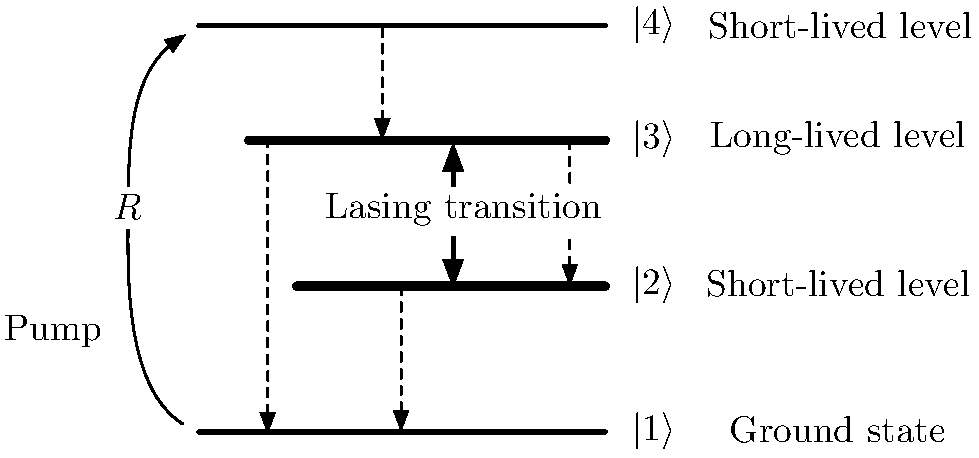
\includegraphics[width=10cm]{4LevelOpticalLaserModel}
    \caption{
        \label{Introduction:4LevelOpticalLaserModel}
        FIXME: This is not a caption.  Figure shamelessly plagiarised from Figure 13.2-6 of \citep{SalehTeich}.  Note that all levels have been incremented by 1 to avoid confusion with the vacuum state.  Figure needs clarifying, but can stand in for the present.
    }
\end{figure}

A pumping mechanism contains excitations that can each increase the occupation of the lasing mode by one.  These excitations are replenished at a finite rate, limiting the rate at which the lasing mode may be increased.  For example, in the 4-level photon laser model illustrated in \figureref{Introduction:4LevelOpticalLaserModel}, atoms are pumped from the ground state $\ket{1}$ to the short-lived state $\ket{4}$ at a rate $R$.  The atoms in state $\ket{4}$ may decay into the $\ket{3}$ state, the excited state of the lasing transition.  The occupation of the lasing mode can therefore not be increased at a rate greater than $R$.  Any physical pumping mechanism will also exhibit saturation, and therefore the laser mode will exhibit gain-narrowing.

Another necessary property of the pumping mechanism is that it be irreversible; once the occupation of the lasing mode has been increased, the probability that the process will reverse should be negligible.  This is achieved by coupling to a large number of essentially-empty modes known as a \emph{reservoir}.  In the case of the 4-level photon laser model depicted in \figureref{Introduction:4LevelOpticalLaserModel}, once an atom in the excited state of the lasing transition, $\ket{4}$ has undergone spontaneous emission into the $\ket{2}$ state, it rapidly decays into the ground state $\ket{1}$.  By ensuring that the ground state of the lasing transition $\ket{2}$ decays to the true ground state $\ket{0}$ faster than it can absorb a lasing photon, the pumping process is made irreversible.  The reservoir is comprised of the essentially-empty modes of the $\ket{2}$ level, which are kept empty due to their short lifetime.

Finally, in many circumstances it is desirable that the photon laser have only one lasing mode.  It is possible for a laser to support more than one lasing mode as the resonator may support many different modes, and if the gain bandwidth of the pumping mechanism encompasses more than one of these modes, multiple lasing modes may result.  As the photon--photon interaction is negligible, these lasing modes do not directly interact, and may operate independently.  Multiple-mode operation in a photon laser is naturally suppressed if the pumping process is \emph{homogeneously broadened}.  In homogeneously broadened gain media, every excitation of the pumping mechanism contributes to the gain of the lasing modes in the same way, i.e.\ every excitation has the same gain profile.  If the gain medium is \emph{inhomogeneously broadened}, some classes of pumping excitations will contribute differently to the total gain profile than others.  A classic example of this is Doppler-broadening.  Atoms in a gain medium will have a finite temperature, and their motion affects what frequencies they are resonant with in the laboratory frame due to the Doppler effect.  If the size of this frequency is greater than the natural width of the lasing transition, the saturation of those excitations resonant with one lasing mode may not affect the gain experienced by another lasing mode.  In this case, both lasing modes will experience gain independently, each without saturating the other.  If the pumping process is inhomogeneously broadened, undesirable modes can be removed by increasing their loss in the optical resonator.  This is naturally achieved by the addition of a second, smaller cavity inside the resonator that is only resonant with the desired mode.  If the pumping process is homogeneously broadened however, while multiple modes may initially experience gain, only the mode with the largest net gain will survive as the gain saturates, resulting in single-mode operation.


\subsubsection{The atom laser}

\begin{figure}
    \centering
    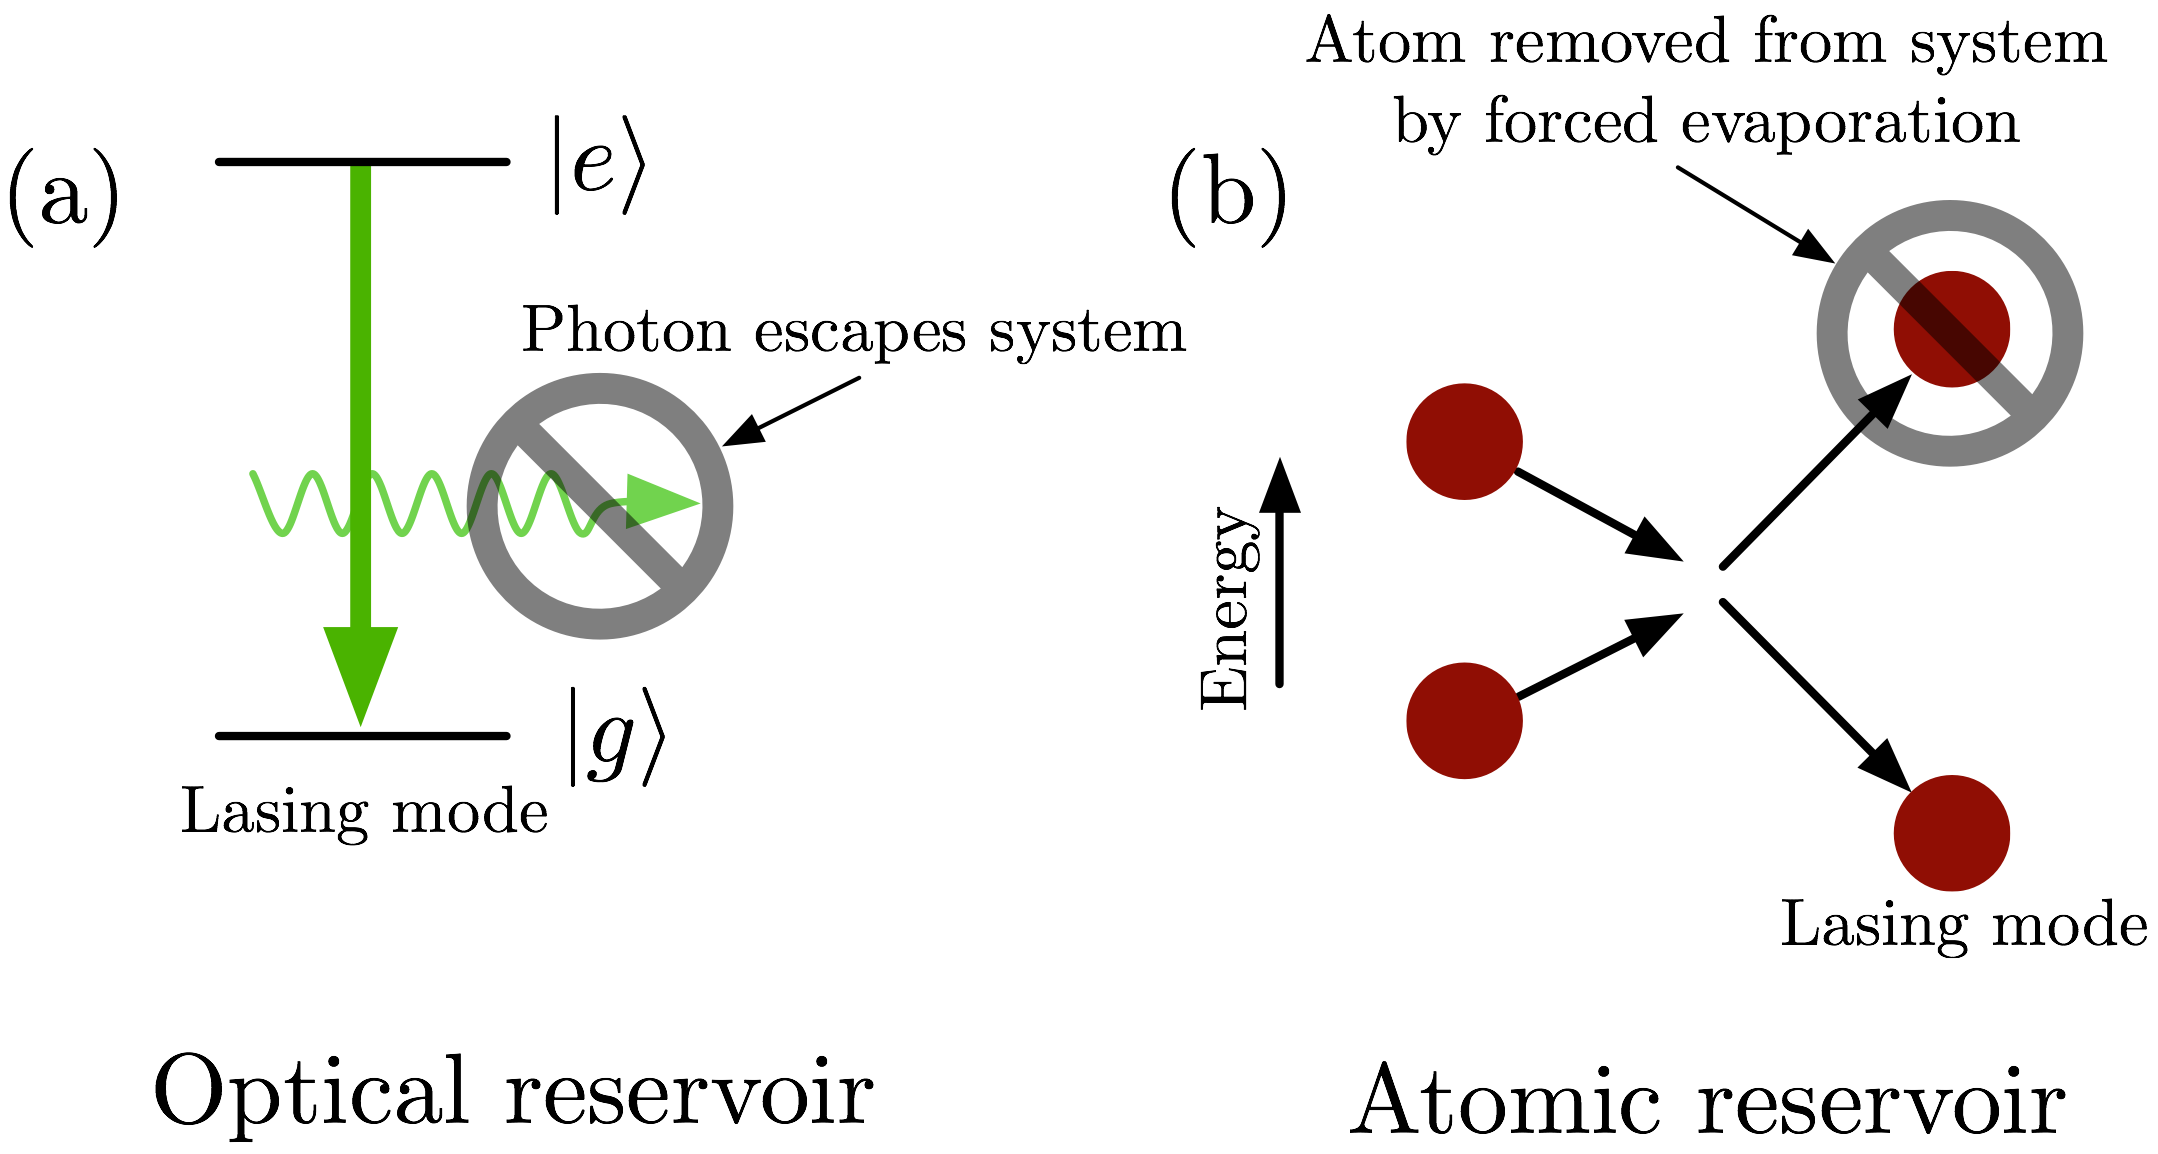
\includegraphics[width=10cm]{ReservoirChoices}
    \caption{
        \label{Introduction:ReservoirChoices}
        Classes of pumping mechanism for an atom laser as defined by the reservoir. FIXME: This is not a caption.
    }
\end{figure}

There are two choices of reservoir for the pumping mechanism of an atom laser: the empty modes of the optical field, or the empty modes of the atomic field.  Each choice corresponds to a different class of pumping mechanism.  These two classes are illustrated in \figureref{Introduction:ReservoirChoices}.  In the first, an atom in an excited internal state is brought into resonance with the lasing mode such that it can decay into the lasing mode.  It is Bose-stimulated to do so by the occupation of the atomic lasing mode.  Once the emitted photon leaves the system, this decay is irreversible.  In the second, two atoms scatter into different energy states, one goes into the lasing mode, while the other gains sufficient energy to be removed from the system (for example, due to forced evaporation, the same process used in the formation of BEC).

Single-mode operation is not simply desirable for an atom laser, it is necessary.  Due to the large interatomic interactions, multiple lasing modes in an atom laser could not operate independently.  Significant scattering would occur between the lasing modes, increasing the linewidth of both, possibly destroying any laser-like qualities in the process.  While the interatomic interactions can be `switched off' with the use of a Feschbach resonance\footnote{FIXME: Missing citation.}, the loss processes are such that higher energy modes experience \emph{less} loss than the lower modes in this case, making the atom laser unstable \citep{Haine:2002kp}.  This instability can be resolved by increasing the interatomic interactions \citep{Haine:2002kp}, adding a position-dependent loss near the edge of the lasing mode \citep{Kneer:1998fk}, and in the case of non-zero interatomic interactions, by increasing the pumping rate \citep{Robins:2001pd}.

In all of the phenomenological atom laser pumping models discussed in the previous paragraph \citep{Haine:2002kp,Kneer:1998fk,Robins:2001pd}, the gain mechanism was effectively `homogeneously broadened' in the sense that all pumping excitations could contribute equally to the gain of all modes.  This is more difficult to achieve for atom lasers than for photon lasers.  In the case of photon lasers, the dispersion relation (the expression for energy --- or equivalently, frequency --- as a function of wavenumber) for the reservoir is relatively flat by comparison to that of the lasing mode.  This is a useful property, as a greater number of pumping excitations can increase the occupation of the lasing mode if variations in the momentum difference between the pumping excitations and the lasing mode can be compensated for by the reservoir with minimal energy cost.  In the limit of a perfectly flat dispersion relation for the reservoir, any momentum difference between the pumping excitation and the lasing mode can result in gain provided only energy is conserved, and due to the finite lifetime of the pumping excitation, energy need only be conserved to within this lifetime.  As a concrete example, consider the photon laser pumping mechanism illustrated in \figureref{Introduction:4LevelOpticalLaserModel} and the atom laser pumping mechanism illustrated in \figureref{Introduction:ReservoirChoices}(a).  The fundamental difference between these two pumping mechanisms is that for the photon laser, the emitted photon goes into the lasing mode, while for the atom laser, it is the decayed atom that enters the lasing mode.  The decay process of these pumping mechanisms is illustrated in \figureref{Introduction:AtomDecay}.  If a violation of energy conservation is permitted in this process of up to $\pm \Gamma$ where $\Gamma$ is the spontaneous lifetime of the $\ket{e}$ state, excited atoms with a wider range of momenta can contribute gain to the lasing mode in the case of the photon laser than in the case of the atom laser.  Specifically, for the photon laser, the wavenumber of the excited atom in the direction parallel to the lasing mode may vary by
\begin{align*}
    \left(\Delta k_{i,\parallel}\right)_\text{ph} \approx \frac{2 M \Gamma}{\hbar \abs{\vect{k}_\gamma}},
\end{align*}
where $M$ is the mass of the atom.  The wavenumber of the atom in perpendicular directions is unconstrained.  However, for the atom laser, the magnitude of the wavenumber of the excited atom may only vary by (assuming a stationary lasing mode of size $d$)
\begin{align*}
    \left(\Delta \abs{\vect{k}_{i}}\right)_\text{at} \approx \frac{2 \Gamma}{c} + \frac{\pi}{d},
\end{align*}
where the second term is due to the momentum-width of the lasing mode.  For the $\lambda = \unit[633]{nm}$ lasing transition of the Helium-Neon gas laser, $\Gamma = \unit[1.4]{MHz}$ \citep[Table~13.2-1]{SalehTeich}, $M_\text{Ne} = 3.3 \times \unit[10^{-26}]{kg}$, giving $\left(\Delta k_{i,\parallel}\right)_\text{ph} \sim \unit[10^8]{m\textsuperscript{-1}}$ for the photon laser and $\left(\Delta \abs{\vect{k}_{i}}\right)_\text{at} \sim \unit[10^{6}]{m\textsuperscript{-1}}$ for an atom laser with a lasing mode of size $d \sim \unit[10]{\micro m}$.  This difference significantly constrains the possible momentum width of the pumping excitations for the pumping mechanism to operate in the `homogeneously broadened' limit.  If the momentum width of the pumping excitations is greater than this, gain for modes other than the lasing mode will not be saturated by the lasing mode, and these other modes experiencing gain will increase the linewidth of the atom laser.  

\begin{figure}
    \centering
    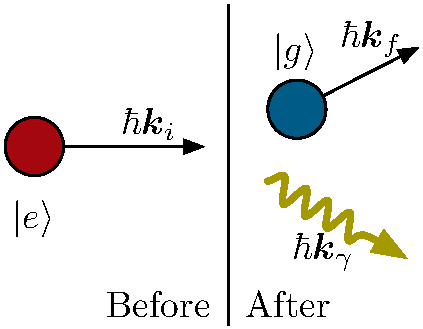
\includegraphics[width=6cm]{AtomDecay}
    \caption{
        \label{Introduction:AtomDecay}
        Excited state atom in the $\ket{e}$ state with momentum $\hbar \vect{k}_i$ decays into an atom in the ground state $\ket{g}$ with momentum $\hbar \vect{k}_f$, and a photon with momentum $\hbar \vect{k}_\gamma$.  In the photon laser pumping mechanism, the photon is in the lasing mode, while in an atom laser pumping mechanism, the decayed atom is in the lasing mode.  FIXME: This is probably not a caption.
    }
\end{figure}

In \chapterref{OpticalPumping}, a pumping mechanism for an atom laser using an optical reservoir is considered.  We attempt to solve the problem of the narrow permissible momentum width of the pumping excitations by making their momentum distribution sufficiently narrow that it can be guaranteed that every atom will be momentum-resonant with the pumping process at some point.  In \chapterref{KineticTheory}, a pumping mechanism using atomic modes as the reservoir is considered.  Although their dispersion relation cannot be considered flat with respect to that of the lasing mode atoms, it is far more so than for photons.  The difficulty with this pumping mechanism is that it is inescapable that thermal atoms will be in the vicinity of the lasing mode.  Scattering between the lasing and thermal atoms will contribute to the collisional broadening of the lasing mode.  Using a Feschbach resonance to cancel these interactions is not an option, as the pumping mechanism itself relies upon interatomic collisions.

\section{Matter wave amplification\dots}

A number of matter-wave amplification processes using the two possible reservoirs have been proposed and demonstrated.  These are discussed in this section.  While none of these matter-wave amplification processes constitute an atom laser pumping mechanism, it is envisaged that an atom laser pumping mechanism would be based on a similar process.

\subsection{\dots\ using an optical reservoir}

A number of previous experiments observing the process of super-radiant Rayleigh scattering seem to offer a physical mechanism for providing pumping through matter-wave amplification \citep{Inouye:1999ph,Kozuma:1999pi}.  Super-radiant Rayleigh scattering occurs when a far off-resonant laser illuminates an elongated BEC.  A matter-wave grating forms along the long axis of the BEC and atoms are preferentially scattered into non-stationary momentum states.  By providing a moving `seed', researchers were able to demonstrate pulsed coherent amplification via the Rayleigh super-radiance mechanism.  However, this type of matter-wave amplification is a transient phenomena, observed over timescales ranging from tens \citep{Inouye:1999ph} to hundreds of microseconds \citep{Kozuma:1999pi}.  On longer timescales, scattering into successively higher momentum modes seems unavoidable \citep{Zobay:2006}, resulting in a `fan'-shaped scattering pattern \citep{Inouye:1999yq}.

Two promising mechanisms for providing a pumping mechanism consistent with a continuous atom laser have recently been demonstrated.  The first is far-detuned stimulated Raman scattering \citep{Schneble:2004,Yoshikawa:2004}, in which atoms in one internal atomic state are Bose-stimulated to make transitions into an alternative atomic state.  The second, reported by \citet{Ginsberg:2007fk}, is a resonant coupling driven by electromagnetically-induced transparency (EIT), demonstrated as stimulated decay of atom pulses into a condensate in a freely falling frame in the context of quantum information processing.  In both cases, the coupling from the source mode is irreversible and the laser mode is dark to the photons produced by the stimulated transitions.

In \chapterref{OpticalPumping}, we consider a pumping mechanism for an atom laser derived from the Raman superradiance and EIT matter-wave amplification processes.  A discussion of related theoretical proposals is given in that chapter.

% \subsubsection{Theoretical proposals}
% 
% There have been several theoretical proposals for atom laser pumping mechanisms that use optical reservoirs.  Several of these\footnote{FIXME: Missing citations.} operate in the Lamb-Dicke limit in which the lasing mode is significantly smaller than the wavelength of the photons they emit.  This is a difficult regime to reach, and it requires the use of a Feschbach resonance to make interatomic interactions negligible if the lasing mode is to be operated with even relatively modest lasing mode occupations $N_0 \gtrsim 10^2$ \citep{Cirac:1994}.  This is an experimental difficulty, but not an insurmountable one.  There are other difficulties with these proposals that are more fatal.
% 
% \citet{Spreeuw:1995} propose trapping atoms in a repulsive optical lattice.  Loss due to off-resonant scattering from the optical trapping beams is greater for the higher-energy states of each lattice site as these states penetrate the repulsive trapping potential more than the lower-energy states.  This gives this proposal the favourable property that loss from higher-energy states is greater than that for lower-energy states, a property difficult to achieve in some circumstances (see \sectionref{Introduction:ThePumpingMechanism}).  However, this proposed pumping mechanism requires that the characteristic energy of the thermal source atoms $k_B T \lesssim \hbar \omega$, where $\omega$ is the trapping frequency of the lattice sites.  As this is also the energy separation between the trapped levels, this must be significantly less than the trap depth, thus requiring that the thermal clouds be isolated to each lattice site.  Each lattice site would therefore operate as independent atom lasers with random relative phases.  The outcoupled mode from this system would therefore not have the coherence properties desired of an atom laser.
% 
% \citep{Cirac:1994} consider a closed system, and optical cooling of a thermal cloud in a system in the LDL.  
% 
% 
% The desire in the LDL is to optically cool to form an atom laser
% 
% \citep{Cirac:1994} is another model in the LDL, which is based upon coherent pumping, and spontaneous decay.  It is also necessary that the degeneracy of the levels is lifted such that reabsorption is not a problem.  This requires that $\Gamma \ll \omega_\text{trap}$, which is a significant requirement.
% 
% A model for an atom laser \citep{Olshanii:1996} --- Single mode, effective Homogeneous broadening, optical pumping.  Sort of phenomenological model that neglects reabsorption.  Considering the opposite limit to the LDL, but quite phenomenologically.
% 
% Cirac and Lewenstein BAR model \citep{Cirac:1996rr}.  Incoherent pumping, then decay driven.
% 
% Continuous optical loading of a Bose-Einstein condensate \citep{Santos:2001ve} --- Few mode model, Homogeneous broadening.  Optical pumping.


\subsection{\dots\ using an atomic reservoir}

The production of BEC using the standard technique of evaporation \citep{Hess:1986,Ketterle:1996} is a matter-wave amplification process \citep{Luiten:1996,Gardiner:1997uq,Miesner:1998}.  In this process, atoms with energy greater than a threshold are removed from the system, thus reducing the mean energy of the system.  Elastic collisions between the remaining atoms lead to rethermalisation at a lower temperature.  This process has been experimentally demonstrated to give exponential gain of the condensate mode until the thermal cloud becomes significantly depleted \citep{Miesner:1998}.

Four-wave mixing of matter-waves \citep{Deng:1999qy} is a fundamentally similar process in which two atoms undergo a collision and scatter into different momentum modes.  When one of the final momentum modes is already occupied, this process is Bose-enhanced, and is a matter-wave amplification process \citep{Vogels:2002}.  If neither of the final momentum modes are occupied, the scattering process gives rise to entanglement between the atoms in the final momentum modes, although only classical correlations have been observed to date \citep{Perrin:2007}.

In \chapterref{KineticTheory}, we consider a pumping mechanism for an atom laser based on evaporation.  In particular, we consider the temperature and flux requirements of the atomic source that must be used to replenish the thermal cloud.


% Theory of an atom laser \citep{Holland:1996mz} --- Single mode, effective Homogeneous broadening, it works, evaporative pumping
% An atom laser based on evaporative cooling \citep{Wiseman:1996} --- Single mode, effective Homogeneous broadening, it work, evaporative pumping
% Theory of a coherent atomic-beam generator \citep{Guzman:1996} ---  Atoms trapped in an optical lattice, interacting via the dipole-dipole interaction.  This dipole-dipole interaction is mediated by the optical lattice.  The dipoles are in fact formed by the optical lattice.  Absent the ac Stark shift, the dipole-dipole interaction would be negligible.  The dipole-dipole interaction therefore occurs whenever \emph{detuned} radiation is present.  In the presence of resonant light, it may be that other effects dominate.  Their simulations are effectively single mode, effective Homogeneous broadening, dipole--dipole interaction with evaporative pumping
% Reducing the Linewidth of an Atom Laser by Feedback \citep{Wiseman:2001zr} --- Single mode model, but demonstrates that some of the linewidth issues can be resolved by feedback
% More feedback reducing the linewidth \citep{Thomsen:2002xc}.

\section{Thesis overview}
FIXME: You can guess the content of this section.  It is relatively unimportant in the scheme of things, and will be written at a later date.


\chapter{Background Theory}
\label{BackgroundTheory}
\graphicspath{{Figures/BackgroundTheory/}{Figures/Common/}}

In this chapter we discuss the theoretical tools and techniques that will be employed in this thesis.  In \sectionref{BackgroundTheory:TransverseProfile}, the results of an application of one of these techniques is discussed.  These results have been published in \citet{Dall:2007}.

\section{Indistinguishability and Bose-Einstein condensation}

All fundamental particles fall into one of two classes determined by their intrinsic spin:  \emph{bosons}, which have integral spin (0, 1, 2, 3, \dots\ in units of $\hbar$), and \emph{fermions}, which have half-integral spin ($\frac{1}{2}$, $\frac{3}{2}$, $\frac{5}{2}$, \dots).  Quantum-mechanically these two classes of particles behave very differently.  Due to a deep property of the relationship between quantum mechanics and (special) relativity known as the spin-statistics theorem \citep{Fierz:1939}, the many-body wavefunction of a system of identical bosons is invariant under particle interchange,
\begin{align}
    \Psi_\text{bosons}(\vect{x}_1, \vect{x}_2, \dots, \vect{x}_i, \dots, \vect{x}_j, \dots, \vect{x}_N) &= \Psi_\text{bosons}(\vect{x}_1, \vect{x}_2, \dots, \vect{x}_j, \dots, \vect{x}_i, \dots, \vect{x}_N), \label{BackgroundTheory:BosonInterchange} \\
    \intertext{while for a system of identical fermions it changes sign,}
    \Psi_\text{fermions}(\vect{x}_1, \vect{x}_2, \dots, \vect{x}_i, \dots, \vect{x}_j, \dots, \vect{x}_N) &= -\Psi_\text{fermions}(\vect{x}_1, \vect{x}_2, \dots, \vect{x}_j, \dots, \vect{x}_i, \dots, \vect{x}_N). \label{BackgroundTheory:FermionInterchange}
\end{align}
The consequence of this difference is that while there may be more than one boson in a mode, there cannot be more than one fermion in any mode.  Were two fermions to occupy the same mode, \eqref{BackgroundTheory:FermionInterchange} would require the wavefunction to be identically zero.  This difference between fermions and bosons is not always noticed however.  At room temperature and pressure the average occupancy of any mode is sufficiently small ($\sim 10^{-6}$ for Helium at $T=\unit[300]{K}$, $p = \unit[10^5]{Pa}$) as to make the probability that one such mode will be multiply-occupied in a bosonic gas entirely negligible.  Under these conditions bosonic and fermionic systems behave identically.

In the previous paragraph it was neglected that Helium is not a fundamental particle, but a \emph{composite} particle.  If the typical energy of particles in a system is sufficiently low that the composite structure of individual particles is not significantly affected during collisions or interactions with other particles, the composite particles may be treated as effectively indivisible.  For the room temperature sample of Helium discussed above, the mean kinetic energy of each atom is $3.9\times\unit[10^{-2}]{eV}$, while the energy required to excite an electron in the atom (and therefore significantly alter the internal state of the atom) is significantly larger at $\unit[20]{eV}$.

Bose-Einstein condensation occurs in the opposite limit in which the lowest energy mode of the system gains a significant fraction of the total population of the system.  This macroscopically-occupied mode is known as the condensate.  Bose-Einstein condensation was originally predicted by Einstein \citep{Einstein:1924,Einstein:1925} in 1924 who was inspired by Bose's description of photons as identical particles symmetric under interchange \citep{Bose:1924}.  Bose showed that it follows from this property, i.e.\ \eqref{BackgroundTheory:BosonInterchange}, that the average occupation of a state with energy $E$ in a system of identical non-interacting bosons is
\begin{align}
    \mean{n(E)} &= \frac{1}{e^{(E - \mu)/k_B T} - 1}, \label{BackgroundTheory:BoseEinsteinDistribution}
\end{align}
where $k_B$ is Boltzmann's constant, $\mu$ is the chemical potential of the system, which is determined by the normalisation condition $N = \sum_i \mean{n(E_i)}$, where $N$ is the number of particles in the system.  If the zero of energy is chosen to be the lowest energy state in the system, the positivity of $\mean{n(0)}$ requires that the chemical potential $\mu$ must be negative.  Equation~\eqref{BackgroundTheory:BoseEinsteinDistribution} is known as the Bose-Einstein distribution and reduces to the classical result $e^{-(E - \mu)/k_B T}$ in the limit that $\abs{\mu} \gg k_B T$, i.e.\ $\mean{n(0)} \ll 1$.  For a gas of Helium at room temperature and pressure, $\mean{n(0)} \approx 10^{-6}$.

Bose-Einstein condensation in weakly-interacting gases occurs below a phase-transition at a critical temperature $T_c$.  In the infinite-particle limit this transition is sharp, however in any real finite system it is smooth.  While Bose-Einstein condensation occurs in a range of systems, the temperature dependence of the condensate occupation depends on the form of the density of states of the system.  The density of states for a free two-dimensional gas is such that a condensate can only form at $T=0$, and so true Bose-Einstein condensation does not occur; while for a free three-dimensional gas the critical temperature is finite and Bose-Einstein condensation occurs for $T < T_c$.  While it was the latter case in which Bose-Einstein condensation was originally derived, most BEC experiments are performed in either magnetic or optical traps, which are approximately harmonic near the trap minimum.  For a Bose gas trapped in a three-dimensional harmonic trap with trapping frequencies $\omega_x$, $\omega_y$ and $\omega_z$ the condensate fraction is \citep{PethickSmith}
\begin{align}
    \frac{N_0}{N} &= \left[1 - \left(\frac{T}{T_c}\right)^{3} \right], \label{BackgroundTheory:CondensateFractionHarmonicTrap}
\end{align}
where $N_0 = \mean{n(0)}$ is the occupation of the ground state, and the critical temperature is given by
\begin{align}
    k_B T_c &\approx 0.94 \hbar \overline{\omega} N^{1/3}, \label{BackgroundTheory:HarmonicTrapCriticalTemperature}
\end{align}
and $\overline{\omega}=(\omega_x \omega_y \omega_z)^{1/3}$ is the geometric mean of the trapping frequencies.  For typical parameters of the $\nucl{87}{Rb}$ experiment considered in this thesis ($N = 5\times 10^5$, $\omega_x = \omega_y = 2 \pi \times \unit[130]{Hz}$, $\omega_z = 2 \pi \times \unit[13]{Hz}$), $T_c \approx \unit[220]{nK}$.  At the critical temperature the condensate is unoccupied ($N_0 \approx 0$), however the condensate occupation increases sharply with decreasing temperature until all particles are in the ground state\footnote{Technically this is only true for a gas of non-interacting bosons.  For weakly-interacting bosons, a non-zero fraction of the atoms are not in the condensate at $T=0$.  However this fraction has never been significantly greater than 1\% in experiments with ultracold gases \citep{Leggett:2001}.  The condensate depletion is neglected in this thesis.} at $T = 0$.  In this limit all particles in the system are in the same single-particle mode and the many-body wavefunction of the system is
\begin{align}
    \Psi(\vect{x}_1, \vect{x}_2, \dots, \vect{x}_N) &= \prod_{i=1}^{N} \phi(\vect{x}_i), \label{BackgroundTheory:ManyBodyWavefunction}
\end{align}
where $\phi(\vect{x})$ is the macroscopically-occupied mode.  In \sectionref{BackgroundTheory:GrossPitaevskiiEquation}, a more accurate description of the state of a BEC will be considered, however \eqref{BackgroundTheory:ManyBodyWavefunction} is a useful approximation in many circumstances.

\section{Hamiltonian}

After second-quantisation \citep{Shankar:1994}, the Hamiltonian describing an interacting multi-component field of bosonic atoms is
\begin{align}
    \label{BackgroundTheory:BasicHamiltonian}
    \begin{split}
        \hat{H} &=
            \sum_i \int d \vect{x}\, \hat{\Psi}_i^\dagger(\vect{x}) \left(- \frac{\hbar^2\nabla^2}{2 M} + V_{i}(\vect{x}) \right) \hat{\Psi}_i^{\phantom{\dagger}}(\vect{x})\\
            &+ \frac{1}{2}\sum_{i j m n} \int \int d\vect{x}\, d\vect{x}'\, \hat{\Psi}_i^\dagger(\vect{x}) \hat{\Psi}_j^\dagger(\vect{x}') V_{ijmn}(\vect{x} - \vect{x}') \hat{\Psi}_m^{\phantom{\dagger}}(\vect{x}') \hat{\Psi}_n^{\phantom{\dagger}}(\vect{x}),
    \end{split}
\end{align}
where $\hat{\Psi}_i(\vect{x})$ is the bosonic annihilation operator that removes an atom of mass $M$ in the internal state $i$ at position $\vect{x}$.  These fields obey the commutation relations
\begin{align}
    \left[\hat{\Psi}_i(\vect{x}),\, \hat{\Psi}_j(\vect{x}') \right] &= 0\\
    \left[ \hat{\Psi}_i^{\phantom{\dagger}}(\vect{x}),\, \hat{\Psi}_j^{\dagger}(\vect{x}')\right] &= \delta_{ij} \delta(\vect{x} - \vect{x}').
\end{align}
The potential $V_i(\vect{x})$ describes the external potential experienced by atoms in the internal state $i$, and includes contributions from gravity and any optical or magnetic trapping fields present.  A common example encountered in this thesis is the cylindrically symmetric harmonic trap of the form
\begin{align}
    V(\vect{x}) &= \frac{1}{2} M \left(\omega_r^2 x^2 + \omega_r^2 y^2 + \omega_z^2 z^2 \right),
\end{align}
where $\omega_r$ is the radial trapping frequency, and $\omega_z$ is the trapping frequency in the $z$ direction.  In this thesis $\omega_r$ is always significantly larger than $\omega_z$.  In this case, $x$ and $y$ are referred to as the `tight' trapping dimensions, and $z$ the `weak' trapping dimension.

The interatomic interaction potential $V_{ijmn}(\vect{x})$ describes scattering processes between two particles in the $m$ and $n$ internal states separated by $\vect{x}$ that scatter into the $i$ and $j$ internal states.  If the atoms have only a single internal state, this is simply the interatomic potential.

Atoms do, however, have internal structure: the quantum numbers $n$, $l$ and $m_l$ for the orbit of each electron; the projections $m_s$ for the spin of each electron; and the quantum numbers describing the state of the atom's nucleus.  Due to the couplings between these different states, none of these are `good' quantum numbers in the sense that they label eigenstates of the Hamiltonian for a single atom.  The set of good quantum numbers depends on the regime in which the experiment is operated.  In the limit of weak magnetic fields, which is the only case encountered in this thesis, the good quantum numbers are the principal quantum number for the outermost electron $n$, the total electronic orbital angular momentum $L$, the total electronic spin $S$, the total electronic angular momentum $J$, the nuclear spin $I$, the total atomic angular momentum $F$, and its projection $m_F$ \citep{Bergmann:1997}.  

In practice most of the quantum numbers that determine the internal atomic state are constant for experimentally-relevant states, and are omitted when describing the atomic states.  For alkali gases, the experimentally-relevant states fall into two classes: long-lived `ground' states, and optically-accessible states which rapidly decay to the `ground' states.  The former are completely determined by the quantum numbers $F$ and $m_F$ (e.g.\ $\ket{F=1, m_F=-1}$ denotes the magnetically-trapped $\ket{n=5, L=0, S=\frac{1}{2}, J = \frac{1}{2}, I=\frac{3}{2}, F=1, m_F=-1}$ state of \nucl{87}{Rb}), while the optically-accessible excited states are determined by the quantum numbers $J$, $F$ and $m_F$.  For the alkali gases the quantum number $J$ may take two values, $J = \frac{1}{2}$ and $J = \frac{3}{2}$.  Due to the fine-structure splitting between states with different values of $J$ ($\unit[7]{THz}$ for \nucl{87}{Rb}), only excited states with a single value of $J$ are typically accessed in a given experiment.  The states with $J=\frac{3}{2}$ are the most relevant experimentally as these have a closed transition with the ground states ($\ket{F=2, m_F=2} \leftrightarrow \ket{J=\frac{3}{2}, F'=3, m_F=3}$ for atoms with $I=\frac{3}{2}$, such as \nucl{87}{Rb}), which can be used for optical cooling and trapping \citep{Metcalf:1999}.  As only a single value of $J$ describes the excited states accessed in a given experiment, the excited states are typically denoted only by the quantum numbers $F$ and $m_F$, with the $F$ quantum number primed to distinguish it from the ground states as in $\ket{F'=3, m_F=3}$.  This notation is used in this thesis, with the excited states belonging to the $\text{D}_2$ transition.

It is the internal structure of atoms that enables them to be manipulated using a rich variety of techniques.  In the presence of a magnetic field, the different $m_F$ levels have different energies separated by the Zeeman splitting.  This enables atoms in certain $m_F$ levels to be trapped in a local magnetic field minimum.  In the presence of radio-frequency radiation resonant with this Zeeman splitting, the $m_F$ levels within a given $F$ manifold are coupled, causing a transfer of population between levels.  In the presence of intense optical radiation far-detuned from resonant transitions, depending on the polarisation, all $m_F$ levels can receive the same energy shift and be trapped equally.  In the presence of pairs of optical fields, momentum can be coherently transferred to the atoms, and depending on the polarisations, simultaneously change their internal state.  The atom--light coupling term is discussed in detail in \sectionref{OpticalPumping:MultimodeModel}.

In the absence of additional coupling terms, the equations of motion for the atomic field operators $\hat{\Psi}_i$ are determined by the Hamiltonian \eqref{BackgroundTheory:BasicHamiltonian},
\begin{align}
    \begin{split}
    i \hbar \frac{\partial}{\partial t}\hat{\Psi}_i(\vect{x}) &= \left( - \frac{\hbar^2 \nabla^2}{2 M}  + V_i(\vect{x}) \right) \hat{\Psi}_i(\vect{x}) \\
        &+ \sum_{jmn} \int d \vect{x}'\, V_{ijmn}(\vect{x} - \vect{x}') \hat{\Psi}_j^\dagger(\vect{x}') \hat{\Psi}_m^{\phantom{\dagger}}(\vect{x}') \hat{\Psi}_n(\vect{x}).
    \end{split}\label{BackgroundTheory:NonLocalOperatorEvolution}
\end{align}
The most complicated part of this evolution is the non-local term governed by the interatomic interaction potential $V_{ijmn}(\vect{x})$.  The following section discusses an approximation in which this potential may be approximated by a \emph{local} interaction, simplifying the evolution described by \eqref{BackgroundTheory:NonLocalOperatorEvolution}.

\section{Atomic scattering}
\label{BackgroundTheory:AtomicScattering}

The Hamiltonian \eqref{BackgroundTheory:BasicHamiltonian} neglects the composite structure of atoms, approximating atoms with different internal states as different `fundamental' particles.  This Hamiltonian is therefore an effective field theory, which is only valid on length scales larger than the atomic size.  At the low temperatures and densities typical of ultracold atom experiments, these structures are not probed, and the effective field theory is a good approximation.  Indeed, it is usual that the details of the interaction potential $V_{ijmn}(\vect{x})$ are not probed either, and the potential can be approximated by a contact interaction \citep{Leggett:2001}
\begin{align}
    V_{ijmn}(\vect{x}) &\approx U_{ijmn} \delta(\vect{x}), \label{BackgroundTheory:ContactInteractionPotential}
\end{align}
where $U_{ijmn} = 4 \pi \hbar^2 a_{ijmn}/M$, and $a_{ijmn}$ is the scattering length for the corresponding interaction.  The scattering length is chosen to reproduce the long-range scattering behaviour of the exact potential $V_{ijmn}(\vect{x})$.  Equation~\eqref{BackgroundTheory:ContactInteractionPotential} is known as the $s$-wave scattering approximation, as only collisions in which the atoms have zero relative motional angular momentum occur.  This neglects collisions between particles having non-zero relative angular momentum that would occur due to the finite extent of the full potential.  These collisions contribute negligibly at the temperatures typical of ultracold atom experiments (particularly for non-polar particles), as atoms with non-zero relative motional angular momentum cannot approach sufficiently closely for $V_{ijmn}(\vect{x})$ to be non-negligible.

In alkali atoms there are two ground-state $F$ manifolds\footnote{An $F$ manifold is a set levels sharing all quantum numbers except $m_F$.  An example is the $F=1$ manifold of \nucl{87}{Rb}, which contains $\ket{F=1, m_F=1}$, $\ket{F=1, m_F=0}$, and $\ket{F=1, m_F=-1}$.}, which are separated by the hyperfine splitting.  The energy difference between these two manifolds is sufficiently large that collisions between atoms in the lower manifold cannot scatter atoms into the upper manifold.  As a result of this restriction it can be shown \citep{Ho:1998} that the scattering only depends on the total angular momentum of the colliding atoms.  The interaction term of \eqref{BackgroundTheory:BasicHamiltonian} can be written as
\begin{align}
    \label{BackgroundTheory:QuasimolecularScatteringTerm}
    \hat{H}_\text{int} &= \frac{1}{2}\sum_{S, m_S}  g_S \int d \vect{x}\, \hat{\Xi}^\dagger_{S, m_S}(\vect{x}) \hat{\Xi}^{\phantom{\dagger}}_{S, m_S}(\vect{x}),
\end{align}
where $g_S = 4 \pi \hbar^2 a_S/M$ is the nonlinear interaction strength, and $a_S$ is the $s$-wave scattering length for the total hyperfine spin $S$ channel.  For bosons, the total hyperfine spin $S$ is restricted to even values due to symmetry \citep{Ho:1998}.  The quasi-molecular operator $\hat{\Xi}_{S, m_S}$ is defined in terms of the atomic annihilation operators and the appropriate Clebsch-Gordan coefficients
\begin{align}
    \hat{\Xi}_{S, m_S}(\vect{x}) &= \sum_{m_F, m_F'} \left(F, m_F; F, m_F' \middle| S, m_S \right) \hat{\Psi}_{F, m_F}(\vect{x}) \hat{\Psi}_{F, m_F'}(\vect{x}),
\end{align}
where $\left(j_1, m_1; j_2, m_2 \middle| J, M\right)$ is a Clebsch-Gordan coefficient.  For the metastable noble gases, the interaction term is also in the form of \eqref{BackgroundTheory:QuasimolecularScatteringTerm} as only one $F$ manifold is accessible.  In metastable Helium the scattering lengths $a_S$ differ by 25\%.  The consequences of this difference are considered in \chapterref{Peaks}.  For $\nucl{87}{Rb}$, however, the scattering lengths for collisions between $F=1$ atoms differ by at most 1\% \citep{Kempen:2002}, permitting the approximation $g_0 \approx g_2$.  In this limit the nonlinear interaction Hamiltonian can be written in the simple form
\begin{align}
    \label{BackgroundTheory:SimpleScattering}
    \hat{H}_\text{int} &= \frac{1}{2} U_\text{int} \sum_{ij} \int d \vect{x}\, \hat{\Psi}_i^\dagger(\vect{x}) \hat{\Psi}_j^\dagger(\vect{x}) \hat{\Psi}_j^{\phantom{\dagger}}(\vect{x}) \hat{\Psi}_i^{\phantom{\dagger}}(\vect{x}).
\end{align}

When interatomic scattering is well-described by the simple interaction \eqref{BackgroundTheory:SimpleScattering}, the operator evolution of \eqref{BackgroundTheory:NonLocalOperatorEvolution} may be simplified to
\begin{align}
    i \hbar \frac{\partial}{\partial t} \hat{\Psi}_i(\vect{x}) &= \left( -\frac{\hbar^2 \nabla^2}{2 M} + V_{i}(\vect{x}) + U_\text{int} \sum_{j} \hat{\Psi}_j^\dagger(\vect{x}) \hat{\Psi}_j^{\phantom{\dagger}}(\vect{x}) \right) \hat{\Psi}_i^{\phantom{\dagger}}(\vect{x}). \label{BackgroundTheory:LocalOperatorEvolution}
\end{align}
While the approximation made to the nonlinear interaction term of the Hamiltonian has made these equations local, they cannot be solved exactly for the general case.  In the absence of the nonlinear term the atoms do not interact with one another, and the energy eigenstates do not depend on the number of atoms in the system.  In this limit the field operator $\hat{\Psi}_i$ may be decomposed as
\begin{align}
    \hat{\Psi}_i(\vect{x}, t) &= \sum_j \hat{a}_{ij} \phi_{ij}(\vect{x}, t),
\end{align}
where the $\phi_{ij}(\vect{x}, t)$ are a set of orthogonal basis functions (the single-particle modes) obeying
\begin{align}
    i \hbar \frac{\partial }{\partial t} \phi_{ij}(\vect{x}, t) &= \left( - \frac{\hbar^2 \nabla^2}{2M} + V_i(\vect{x}) \right) \phi_{ij}(\vect{x}, t),
\end{align}
and $\hat{a}_{ij}$ are stationary bosonic annihilation operators for the corresponding single-particle modes.  

With the addition of the nonlinear interaction term, the evolution of the field operator may not be decomposed into the sum of \emph{stationary} bosonic annihilation operators and time-dependent basis functions; the evolution of each `mode' would necessarily depend on the occupation of the other modes.  It is this complication that makes \eqref{BackgroundTheory:LocalOperatorEvolution} difficult to solve in the general case, either analytically \emph{or numerically}.  The difficulty numerically is the sheer amount of information needed to describe $\hat{\Psi}(\vect{x})$.  For a system with $N=100$ atoms that can each occupy one of $m = 100$ spatial modes, $\sim 10^{117}$ complex numbers are needed to describe $\hat{\Psi}(\vect{x})$.  Typical BEC's have $N \gtrsim 10^5$.  This complexity is a double-edged sword: it is what gives quantum computers their tremendous potential, but it is also what makes it hard to solve many-body interacting quantum problems with classical computers.

The following section discusses a limit in which the field operator can be approximated by a complex function, whose evolution can feasibly be simulated numerically.

\section{The Gross-Pitaevskii equation}
\label{BackgroundTheory:GrossPitaevskiiEquation}

For the moment, we consider the simpler case of a single-component atomic field $\hat{\Psi}(\vect{x})$.

As the difficulty in solving the evolution equation \eqref{BackgroundTheory:LocalOperatorEvolution} lies in its operator nature, we may seek to simplify the problem by considering its expectation value instead,
\begin{align}
    i \hbar \frac{\partial}{\partial t} \mean{\hat{\Psi}(\vect{x})} &= - \frac{\hbar^2 \nabla^2}{2 M} \mean{\hat{\Psi}(\vect{x})} + V(\vect{x})\mean{\hat{\Psi}(\vect{x})} + U_\text{int} \mean{\hat{\Psi}^\dagger (\vect{x}) \hat{\Psi}(\vect{x}) \hat{\Psi}(\vect{x})}. \label{BackgroundTheory:ExpectationValueEvolution}
\end{align}
This equation certainly does not contain all of the information about the quantum field $\hat{\Psi}(\vect{x})$; at best it can describe classical properties of the condensate such as its density and mean local velocity.  Neither is it a closed system; \eqref{BackgroundTheory:ExpectationValueEvolution} cannot be solved without knowing the evolution of the higher-order expectation value $\mean{\hat{\Psi}^\dagger(\vect{x}) \hat{\Psi}(\vect{x}) \hat{\Psi}(\vect{x})}$.  This higher-order expectation value should be well-approximated by $\abs{\mean{\hat{\Psi}(\vect{x})}}^2\mean{\hat{\Psi}(\vect{x})}$ in the limit that the atomic field $\hat{\Psi}(\vect{x})$ has a large classical component,
\begin{align}
    \hat{\Psi}(\vect{x}) &= \Psi(\vect{x}) + \delta\hat{\Psi}(\vect{x}), \label{BackgroundTheory:FieldOperatorDecomposition}
\end{align}
where $\Psi(\vect{x}) = \mean{\hat{\Psi}(\vect{x})}$, and $\delta\hat{\Psi}(\vect{x})$ is `small' in some sense (e.g. $\mean{\delta\hat{\Psi}^\dagger(\vect{x}) \delta\hat{\Psi}(\vect{x})} \ll \abs{\Psi(\vect{x})}^2$).  In this limit, certain quantum-mechanical properties such as entanglement have been neglected, however as the system is described in terms of an atomic field amplitude (and not a density), Eq.~\eqref{BackgroundTheory:ExpectationValueEvolution} will include single-particle interference phenomena; it is a semi-classical description of a BEC.

We might expect that the description of the BEC by the many-body wavefunction \eqref{BackgroundTheory:ManyBodyWavefunction} includes a large classical component in the sense defined above as all $N$ particles are in the same single-particle mode $\phi(\vect{x})$.  In this case the expectation value of the field operator is
\begin{align}
    \mean{\hat{\Psi}(\vect{x})} &= \left<N, 0, 0, \dots \middle| \hat{\Psi}(\vect{x}) \middle| N, 0, 0, \dots \right> \notag \\
    &= \left<N, 0, 0, \dots \middle| \sqrt{N} \phi(\vect{x}) \middle| N - 1, 0, 0, \dots \right> \notag \\
    &= 0. \label{BackgroundTheory:OperatorExpectationValueNumberState}
\end{align}
This perhaps unexpected result is a consequence of the symmetry of the initial state: the state is unchanged if the single-particle mode $\phi(\vect{x})$ is modified by an arbitrary global phase $\phi(\vect{x}) \mapsto e^{i \theta}\phi(\vect{x})$.  This symmetry is preserved by the Hamiltonian \eqref{BackgroundTheory:BasicHamiltonian} and results from conservation of the total number of atoms in the system.

If we suppose for the moment that it is possible to create states that do not possess this symmetry, the BEC could instead be in the coherent state $\ket{\Psi(\vect{x})}$, with the expectation value of the field operator acquiring the non-zero value
\begin{align}
    \mean{\hat{\Psi}(\vect{x})} &= \Psi(\vect{x}). \label{BackgroundTheory:NonZeroMeanField}
\end{align}
In this case, \eqref{BackgroundTheory:ExpectationValueEvolution} becomes
\begin{align}
    i \hbar \frac{\partial}{\partial t} \Psi(\vect{x}) &= \left(- \frac{\hbar^2 \nabla^2}{2 M} + V(\vect{x}) + U_\text{int} \abs{\Psi(\vect{x})}^2 \right) \Psi(\vect{x}), \label{BackgroundTheory:GrossPitaevskii}
\end{align}
where the condensate expectation value $\Psi(\vect{x})$ has normalisation $N = \int d \vect{x}\, \abs{\Psi(\vect{x})}^2$.  Equation~\eqref{BackgroundTheory:GrossPitaevskii} is known as the Gross-Pitaevskii (GP) equation.  

It has been assumed in deriving the GP equation that the condensate will remain in a coherent state.  This is an approximation as the nonlinear scattering term gives rise to collapse and revival of the global phase, exactly as occurs in the case of the anharmonic oscillator (see \sectionref{BackgroundTheory:StochasticPhaseSpaceMethods}).  This effect has been observed in BECs held in optical lattices \citep{Greiner:2002fk}, however the time-scale for collapse when BECs are held in magnetic or optical dipole traps is much larger than typical experimental timescales.  For a \nucl{87}{Rb} condensate of $N= 5 \times 10^5$ atoms held in a trap with trapping frequencies $\omega_r = 2\pi\times\unit[130]{Hz}$ and $\omega_z = 2\pi \times \unit[13]{Hz}$, the time-scale for the collapse of the global phase is $\unit[120]{ms}$, significantly longer than typical experimental timescales of the order of tens of milliseconds.

It must be stated at this point that the BEC cannot be created with the kind of broken phase-symmetry necessitated by \eqref{BackgroundTheory:NonZeroMeanField}.  A coherent state is a particular superposition of number states,
\begin{align}
    \ket{\alpha} &= e^{-\frac{1}{2} \abs{\alpha}^2} \sum_{n=0}^{\infty} \frac{\alpha^n}{\sqrt{n!}} \ket{n},
\end{align}
however any Hamiltonian that conserves number cannot couple states of different total number, and therefore cannot affect the phase differences between these states.  A coherent state therefore cannot be formed by any number-conserving Hamiltonian.

Although derived using the concept of broken-symmetry, it will be shown in the following that the GP equation is a good description of condensates where $\Psi(\vect{x})$ is known as the \emph{order-parameter} of the condensate, and its global phase has no physical significance.

In reality, BECs are not formed in isolation but a large sample of atoms is evaporatively cooled until a much smaller number of atoms remain in a Bose-condensed state.  If the combined system has a total of $N$ atoms, and there is a probability $p$ that each atom may be in the condensate, the state of the system after evaporation is given by
\begin{align}
    \ket{\Psi} &= \sum_{n=0}^N \sqrt{N \choose n}   p^{\frac{n}{2}} \left(1-p\right)^{\frac{N-n}{2}}  e^{i \theta_n} \ket{n}_\text{condensate}\ket{N-n}_\text{rest}, \label{BackgroundTheory:BECBinomialDistribution}
\end{align}
where $\ket{n}_\text{condensate}$ is the state of the condensate with $n$ atoms in it, $\ket{N-n}_\text{rest}$ describes the rest of the system (the evaporated atoms) with $N-n$ atoms, and $\theta_n$ is an arbitrary phase between the different elements of the superposition.  The prefactors in \eqref{BackgroundTheory:BECBinomialDistribution} describe a Binomial distribution where each atom has a probability $p$ of being in the condensate mode.  On average, there will be $N_0 = p N$ atoms in the condensate.  Note that as this state has a fixed total number of atoms $N$, it does not possess any of the unphysical broken symmetry assumed previously.

Once the evaporation process is complete, it is only the condensed part of the system that we are interested in.  This part of the system is described by a reduced density matrix that is obtained by tracing over the rest of the system,
\begin{align}
    \hat{\rho}_\text{condensate} &= \Tr_\text{rest}\left\{ \ketbra{\Psi}{\Psi} \right\} \notag \\
     &= \sum_{n=0}^{N} {N \choose n} p^n (1-p)^{N-n} \left(\ketbra{n}{n}\right)_\text{condensate} \notag \\
     &\approx \sum_{n=0}^{\infty} \frac{N_0^n e^{- N_0}}{n!} \left(\ketbra{n}{n} \right)_\text{condensate}, \label{BackgroundTheory:CondensateDensityMatrixPoissonDistribution}
\end{align}
where in the last line we have used the result that in the limit $N\rightarrow \infty$ with $p N = N_0$ fixed, the Binomial distribution approaches a Poisson distribution with mean $N_0$.  Regardless of how one motivates it, \eqref{BackgroundTheory:CondensateDensityMatrixPoissonDistribution} is a reasonable approximation to the state of a BEC produced evaporatively;  it seems unlikely that a lossy process such as evaporation would leave the system in a pure state, either a pure number state or a pure coherent state.  

As a coherent state has a Poisson number distribution, a density matrix which is a Poisson-distributed mixture of number states is equal to a mixture over global phase of coherent states.  Thus:
\begin{align}
    \hat{\rho}_\text{condensate} &= \int_0^{2\pi} \frac{d\theta}{2\pi} \ketbra{e^{i \theta} \Psi(\vect{x})}{e^{i \theta} \Psi(\vect{x})}, \label{BackgroundTheory:CondensateDensityMatrixCoherentStateMixture}
\end{align}
where $\int d \vect{x} \abs{\Psi(\vect{x})}^2 = N_0$.  We now have a description of the condensate in terms of coherent states again, but this representation respects the global phase symmetry enforced by the conservation of total atom number.  

As quantum mechanics is linear in state vectors and density matrices, the components of superpositions and mixtures can be considered \emph{individually} when determining properties of the system.  For example, if the system is in the state $\hat{\rho} = \sum_i p_i \ketbra{\Psi_i}{\Psi_i}$, then the evolution of each $\hat{\rho_i} = \ketbra{\Psi_i}{\Psi_i}$ can be considered individually and expectation values constructed from the weighted expectation values for each $\hat{\rho_i}$.  The expectation value of the operator $\hat{O}$ is
\begin{align*}
    \mean{\hat{O}} &= \Tr\{ \hat{O} \hat{\rho}  \} = \sum_i p_i \big< \Psi_i \big| \hat{O} \big| \Psi_i \big> = \sum_i p_i \Tr\{ \hat{O} \hat{\rho}_i  \}.
\end{align*}
In the context of \eqref{BackgroundTheory:CondensateDensityMatrixCoherentStateMixture}, this means that the evolution of $\ket{e^{i \theta}\Psi(\vect{x})}$ for each $\theta$ may be considered individually.  The evolution of each of these coherent states can be described by the GP equation \eqref{BackgroundTheory:GrossPitaevskii}.  However, as every physical expectation value must conserve total number, they are therefore independent of the global phase $\theta$.  It therefore suffices to solve the GP equation for a single $\theta$.  In particular, the quantity $\hat{\Psi}(\vect{x})$ is \emph{not} a physical observable, and therefore the fact that its expectation value depends on $\theta$ is not a problem.  Physical expectation values such as $\hat{\Psi}^\dagger(\vect{x}) \hat{\Psi}(\vect{x}')$ are independent of $\theta$,
\begin{align}
    \mean{\hat{\Psi}^\dagger(\vect{x}) \hat{\Psi}(\vect{x}')} &= e^{-i\theta}\Psi^*(\vect{x}) e^{i\theta}\Psi(\vect{x}') = \Psi^*(\vect{x}) \Psi(\vect{x}').
\end{align}
The concept of symmetry-breaking in this context is therefore a useful calculational aid, not a fundamental physical principle.    It can be applied provided one understands that the global phase of the coherent state is meaningless.

The concept of spontaneously-broken symmetries is discussed in greater detail elsewhere \citep{Leggett:1991fj,Molmer:1997fr}.  % In principle, if one believed in spontaneous symmetry-breaking then one could use a relative phase standard \citep{Dunningham:1998} to measure the phase difference between successive condensates produced in the same experiment.  In principle, if the experiment is operated identically both times the phase difference between the two condensates should be zero.  In practice, shot-to-shot number fluctuations in experiments exceed that expected due to the poisson distribution.

In the rest of this thesis, the symmetry-breaking assumption will be applied.  It is understood that this is a calculational tool equivalent to assuming the system to be in a state of the form of \eqref{BackgroundTheory:CondensateDensityMatrixCoherentStateMixture}, which preserves the global phase symmetry dictated by total number conservation.

\parasep

The Gross-Pitaevskii equation has been a tremendously successful description of Bose-condensed systems, and has been used to successfully describe a range of phenomenon, including collective excitations of the condensate \citep{Ruprecht:1996,Edwards:1996}, vortex properties and dynamics \citep{Dalfovo:1996,Edwards:1996a,Caradoc-Davies:1999,Caradoc-Davies:2000qy}, expansion of the condensate after trap switch-off \citep{Dalfovo:1997lr}, and soliton dynamics \citep{Burger:1999eu}.  

The nonlinear term of the Gross-Pitaevskii equation prevents it being solved analytically, however the GP equation is tractable numerically.  The following section describes a limit in which the approximate form of the ground state of the GP equation may be obtained.

\subsection{Thomas-Fermi approximation}

The ground state of a condensate is described by the time-independent Gross-Pitaevskii equation \citep{Leggett:2001},
\begin{align}
    \mu \Psi(\vect{x}) &= \left(- \frac{\hbar^2 \nabla^2}{2M} + V(\vect{x}) + U_\text{int} \abs{\Psi(\vect{x})}^2 \right) \Psi(\vect{x}),
\end{align}
where $\mu = \partial \mean{\hat{H}} / \partial N$ is the chemical potential of the condensate.  In the limit that the nonlinear term is zero, the condensate ground state in a harmonic trap is Gaussian,
\begin{align}
    \Psi(\vect{x}) &= \sqrt{N} \left(\frac{M \overline{\omega}}{\hbar \pi} \right)^{\frac{3}{4}} \exp\left[ - \frac{M}{2 \hbar} \left(\omega_x x^2 + \omega_y y^2 + \omega_z z^2\right) \right],
\end{align}
where $\overline{\omega} = \left(\omega_x \omega_y \omega_z\right)^{\frac{1}{3}}$ is the geometric mean of the trapping frequencies.  As the nonlinear term is increased, interatomic repulsion will increase the mean separation of atoms and the ground state will become broader.  For a sufficiently large scattering length, the kinetic energy term in \eqref{BackgroundTheory:GrossPitaevskii} is small in comparison to both the potential and interaction terms as it depends on the second derivative of $\Psi(\vect{x})$.  In the Thomas-Fermi approximation the kinetic energy term is neglected, and the form of the wavefunction may be explicitly obtained,
\begin{align}
    \Psi(\vect{x}) &= 
    \begin{cases}
        \sqrt{\frac{\mu - V(\vect{x})}{U_\text{int}}} &\text{ if } \mu - V(\vect{x}) \geq 0,\\
        0 & \text{ otherwise.}
    \end{cases}
\end{align}
By requiring that $\Psi(\vect{x})$ be correctly normalised, the chemical potential is found to be
\begin{align}
    \mu &= \left(\frac{15 N U_\text{int} \overline{\omega}^3}{8 \pi} \right)^{\frac{2}{5}} \left(\frac{M}{2} \right)^{\frac{3}{5}}. \label{BackgroundTheory:ChemicalPotential}
\end{align}
The Thomas-Fermi approximation is only valid in the limit that the chemical potential given by \eqref{BackgroundTheory:ChemicalPotential} is much larger than the ground state energy of the harmonic trap, i.e.\ $\mu \gg \frac{1}{2} \hbar (\omega_x + \omega_y + \omega_z)$.

\begin{figure}
    \centering
    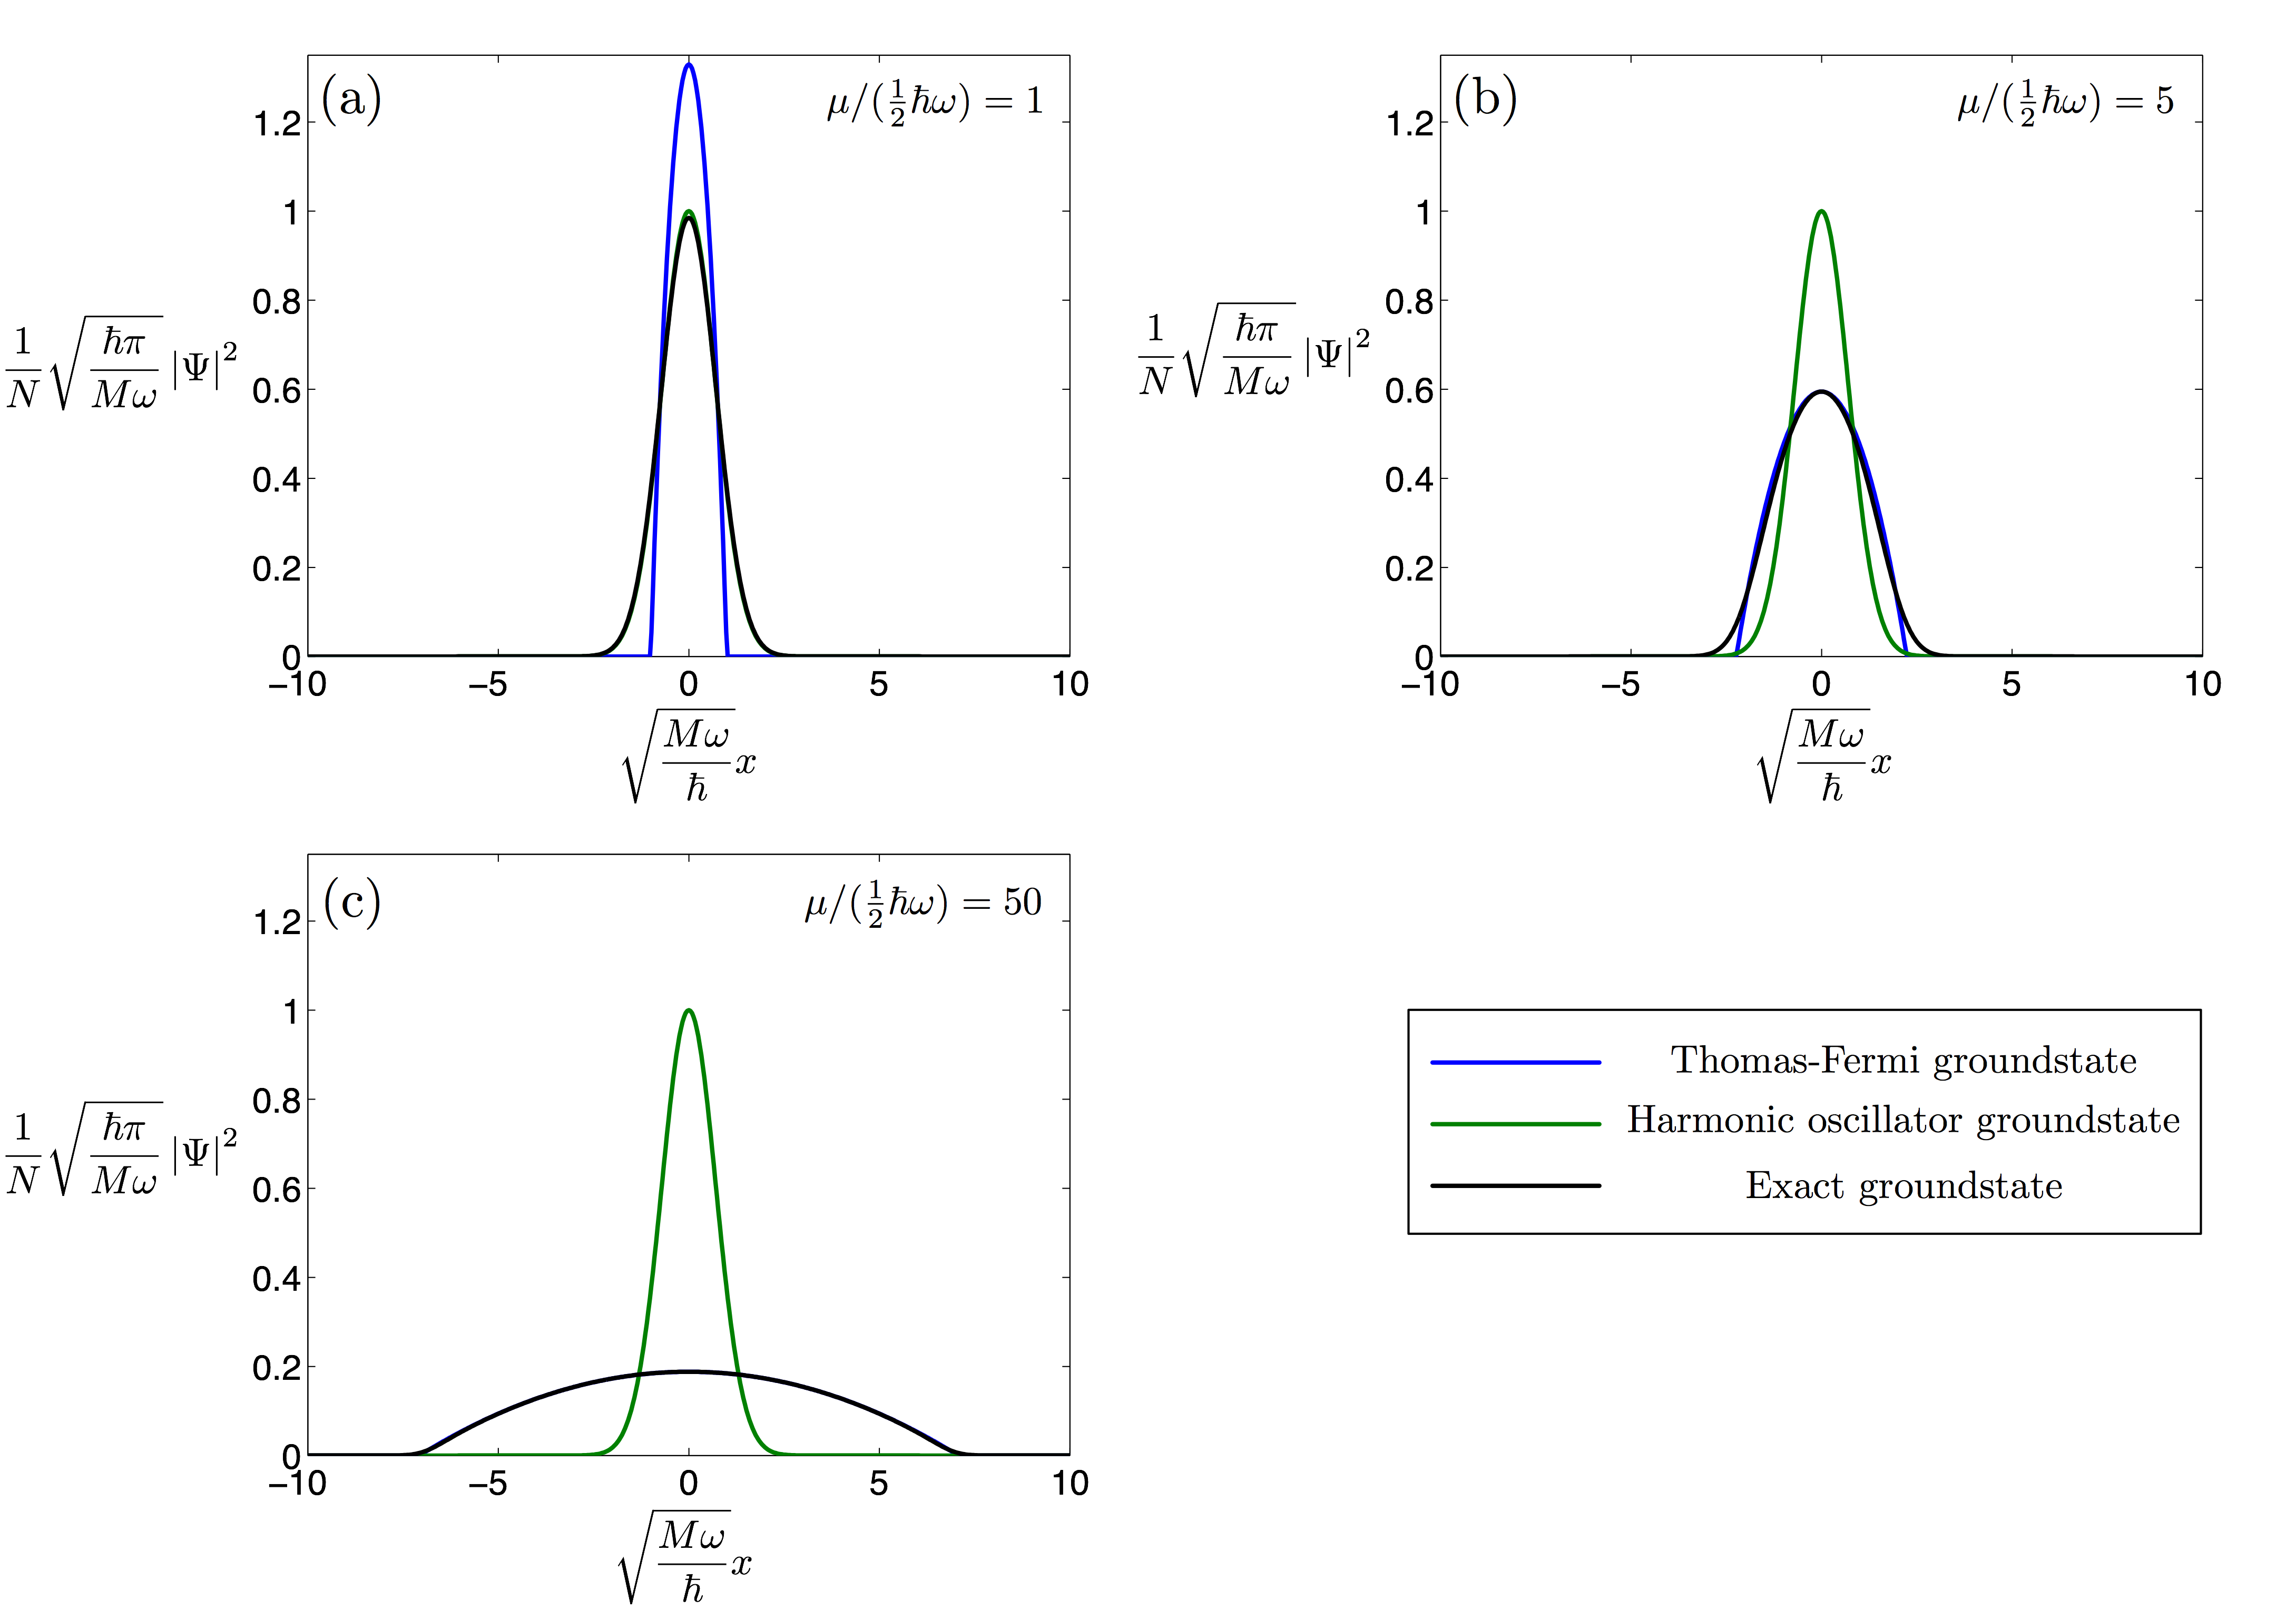
\includegraphics[width=14cm]{GroundStateComparison}
    \caption{Comparison of harmonic oscillator, Thomas-Fermi and exact one-dimensional groundstates in different regimes.  (a) $\mu / (\frac{1}{2} \hbar \omega) = 1$, (b) $\mu / (\frac{1}{2} \hbar \omega) = 5$, (c) $\mu / (\frac{1}{2} \hbar \omega) = 50$.}
    \label{BackgroundTheory:GroundStateComparison}
\end{figure}

A comparison of the harmonic-oscillator and Thomas-Fermi groundstates is given in \figureref{BackgroundTheory:GroundStateComparison}.  The density profile of the Thomas-Fermi wavefunction is that of a truncated inverted parabola.  Near the edge of the wavefunction the Thomas-Fermi approximation breaks down.  There, the nonlinear term is smaller, and the kinetic energy term is larger.  In this region the density profile of the exact groundstate decays smoothly due to the kinetic energy term.  The Thomas-Fermi profile instead has a discontinuous first derivative.  This discontinuity gives rise to a well-defined condensate radius in each dimension given by
\begin{align}
    r_\text{TF} &= \frac{1}{\omega_r} \sqrt{\frac{2 \mu}{M}},
\end{align}
where $\omega_r$ is the trapping frequency of that dimension.

The Thomas-Fermi approximation is useful as a simple description of the condensate when other parts of the system are of primary interest (it is used in this manner in the next section), or as an initial guess when finding the true groundstate of the system numerically.

\subsection{Application: Transverse profile of the atom laser}
\label{BackgroundTheory:TransverseProfile}

As discussed in \sectionref{Introduction:PhotonAndAtomLasers}\footnote{FIXME: We can expect that the idea of an atom laser has been discussed in the introduction.  Check cross-ref at later date.}, an atom laser is formed by outcoupling from a condensate to produce a directional beam of highly coherent atoms.  These atom lasers show great promise for studies of fundamental physics and in high precision measurements \citep{Kasevich:2002}.  For atom lasers to be applied in this way it will be crucial to develop atom lasers with output modes that are as clean as possible in amplitude and phase, to allow stable mode matching, just as it was crucial for optical lasers.  It is therefore important to understand what influences the transverse profile of an atom laser.  In this section, we demonstrate the application of the Gross-Pitaevskii equation to this problem.  The results of this section have been published in \citet{Dall:2007}.

\parasep

For a magnetically-trapped condensate in an $F=1$ manifold, the atoms in one of the $m_F$ Zeeman levels are trapped (the low-field seeking level, either $m_F=1$ as in He* or $m_F=-1$ as in \nucl{87}{Rb}), the atoms in the $m_F=0$ level experience no magnetic trapping potential (and are referred to as `untrapped'), and the atoms in the level opposite to the trapped state experience a repulsive potential and are referred to as `anti-trapped'.  For He*, the potentials experienced by the three levels in a cylindrically-symmetric trap are
\begin{align}
    V_{m_F}(\vect{x}) &= m_F V_\text{trap}(\vect{x}) = m_F \frac{1}{2} M \left(\omega_r^2 x^2 + \omega_r^2 y^2 + \omega_z^2 z^2 \right).
\end{align}
These three levels are coupled by applying radio-frequency radiation resonant with the Zeeman splitting between the $m_F$ levels.  This Zeeman splitting is due to the magnetic trap (and a bias field), and therefore the outcoupling process will be resonant along a surface of constant $V_\text{trap}(\vect{x})$.  Due to gravity, the centre of the condensate is a distance $g/\omega_y^2$ below the centre of the magnetic trap.  For strong traps the outcoupling surfaces will be spheroids approximately concentric with the condensate [see \figureref{BackgroundTheory:OutcouplingSurfaces}(a)], while for weaker traps the outcoupling surfaces will be almost horizontal planes [see \figureref{BackgroundTheory:OutcouplingSurfaces}(b)].  As we shall show, the shape of the outcoupling surface significantly impacts the transverse profile of the atom laser.

\begin{figure}
    \centering
    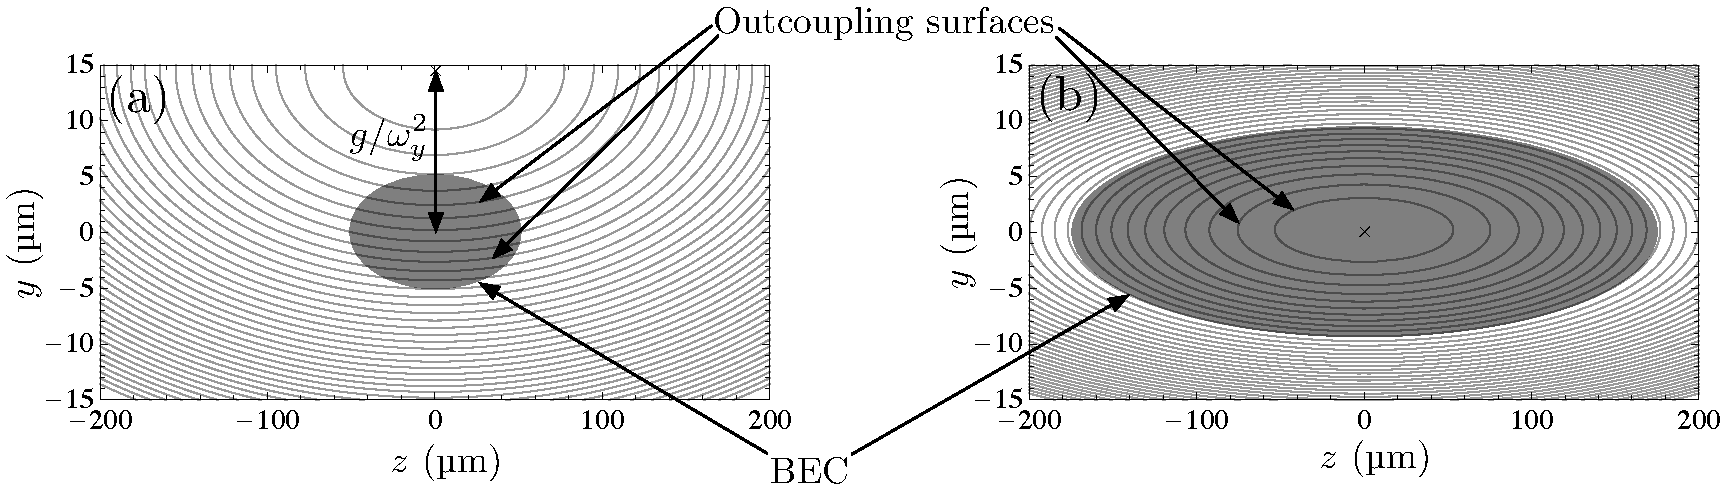
\includegraphics[width=15cm]{OutcouplingSurfaces}
    \caption{Outcoupling surfaces of condensates held in magnetic traps.  Pictured is the size of the Thomas-Fermi condensate and contours of the magnetic trap equally-spaced in energy.  The origin of each coordinate system is the centre of the condensate, and the magnetic trap centres are marked with `$\times$'.  Figure (a) illustrates a condensate for typical parameters of the \nucl{87}{Rb} experiment at the ANU \citep{Jeppesen:2008}; $N = 5 \times 10^5$ atoms, $\omega_r = 2 \pi \times \unit[130]{Hz}$, $\omega_z = 2 \pi \times \unit[13]{Hz}$.  The gravitational sag separating the centre of the condensate from the centre of the magnetic trap is $\Delta y = \unit[15]{\micro m}$.  Figure (b) illustrates a condensate for typical parameters of the He* experiment at the ANU \citep{Dall:2007a,Dall:2007}; $N = 2 \times 10^6$ atoms, $\omega_r = 2\pi \times \unit[1020]{Hz}$, $\omega_z = 2 \pi \times \unit[55]{Hz}$.  The gravitational sag separating the centre of the condensate from the centre of the magnetic trap is $\Delta y = \unit[0.2]{\micro m}$.  The acceleration due to gravity is in the $-y$ direction.  The aspect ratio of this figure is not 1:1 for reasons of clarity; the condensates are significantly more elongated than pictured.}
    \label{BackgroundTheory:OutcouplingSurfaces}
\end{figure}


The equations of motion for the system including the rf coupling is
\begin{subequations}
    \label{BackgroundTheory:AtomLaserF1}
    \begin{align}
        \begin{split}
            i \hbar \frac{\partial}{\partial t} \Psi_1(\vect{x}) &= \left[ - \frac{\hbar^2 \nabla^2}{2 M} + V_\text{trap}(\vect{x}) + M g y + U_\text{int}\left(\abs{\Psi_1}^2 + \abs{\Psi_0}^2 + \abs{\Psi_{-1}}^2\right)\right] \Psi_1(\vect{x})\\
            & + \hbar \Omega \Psi_0(\vect{x}),
        \end{split}\\
        \begin{split}
            i \hbar \frac{\partial}{\partial t} \Psi_0(\vect{x}) &= \left[ - \frac{\hbar^2 \nabla^2}{2 M} + M g y + U_\text{int} \left(\abs{\Psi_1}^2 + \abs{\Psi_0}^2 + \abs{\Psi_{-1}}^2\right)\right] \Psi_0(\vect{x})\\
            & + \hbar \Omega \Psi_1(\vect{x}) + \hbar \Omega \Psi_{-1}(\vect{x}),
        \end{split}\\
        \begin{split}
            i \hbar \frac{\partial}{\partial t} \Psi_{-1}(\vect{x}) &= \left[ - \frac{\hbar^2 \nabla^2}{2 M} - V_\text{trap}(\vect{x}) + M g y + U_\text{int}\left(\abs{\Psi_1}^2 + \abs{\Psi_0}^2 + \abs{\Psi_{-1}}^2\right)\right] \Psi_{-1}(\vect{x})\\
            & + \hbar \Omega \Psi_0(\vect{x}),
        \end{split}
    \end{align}
\end{subequations}
where $\Omega$ is the Rabi frequency.

Initially the condensate is in the ground state of the trapped $m_F=1$ state.  Once the outcoupling is turned on, the states are coupled and atoms are transferred to the $m_F=0$ and $m_F=-1$ levels.  In the limit of weak outcoupling, the atoms in the $m_F=0$ level leave the region in which outcoupling is resonant without being significantly coupled into the $m_F=-1$ level.  The $m_F=-1$ level is therefore relatively unpopulated and may be neglected.  It is the untrapped $m_F=0$ level that we are primarily interested in as the freely-falling atom laser forms in this level.

For short times, most of the atoms are in the $m_F=1$ level and we may use the Thomas-Fermi approximation to determine the effective potential seen by the untrapped $m_F=0$ atoms.  Inside the condensate, the effective potential for the untrapped atoms has contributions from gravity and interatomic interactions,
\begin{align}
    V_\text{eff}(\vect{x}) &= M g y + U_\text{int} \abs{\Psi_1(\vect{x})}^2 = M g y + \left(\mu - V_\text{trap}(\vect{x}) - M g y \right) \notag\\
    &= \mu - V_\text{trap}(\vect{x}).
\end{align}
This effective potential experienced by the untrapped atoms is a repulsive harmonic potential centred at the centre of the magnetic trap.  Once the atoms are outcoupled they therefore accelerate away from the centre of the magnetic trap until they reach the edge of the condensate, whereupon they fall under gravity.

There is a great difference in the behaviour of atoms outcoupled from a weak trap and from a tight trap.  If the outcoupling surfaces are almost horizontal planes [\figureref{BackgroundTheory:OutcouplingSurfaces}(a)], the atoms will be accelerated almost uniformly downwards.  If the outcoupling surfaces are prolate spheroids entirely contained within the condensate [\figureref{BackgroundTheory:OutcouplingSurfaces}(b)], atoms will be expelled in all directions away from the centre of the magnetic trap.  This difference is illustrated in \figureref{BackgroundTheory:HeliumTransverseProfile} which displays the results of 3D GP simulations of the density of the atom laser in the region near the BEC in the cases of a weak trap [$\omega_r = 2\pi \times \unit[50]{Hz}$, $\omega_z = 2\pi \times\unit[50]{Hz}$; \figureref{BackgroundTheory:HeliumTransverseProfile}(a)] and a tight trap [$\omega_r = 2 \pi \times \unit[460]{Hz}$, $\omega_z = 2\pi \times \unit[50]{Hz}$; \figureref{BackgroundTheory:HeliumTransverseProfile}(b)].  

\begin{figure}
    \centering
    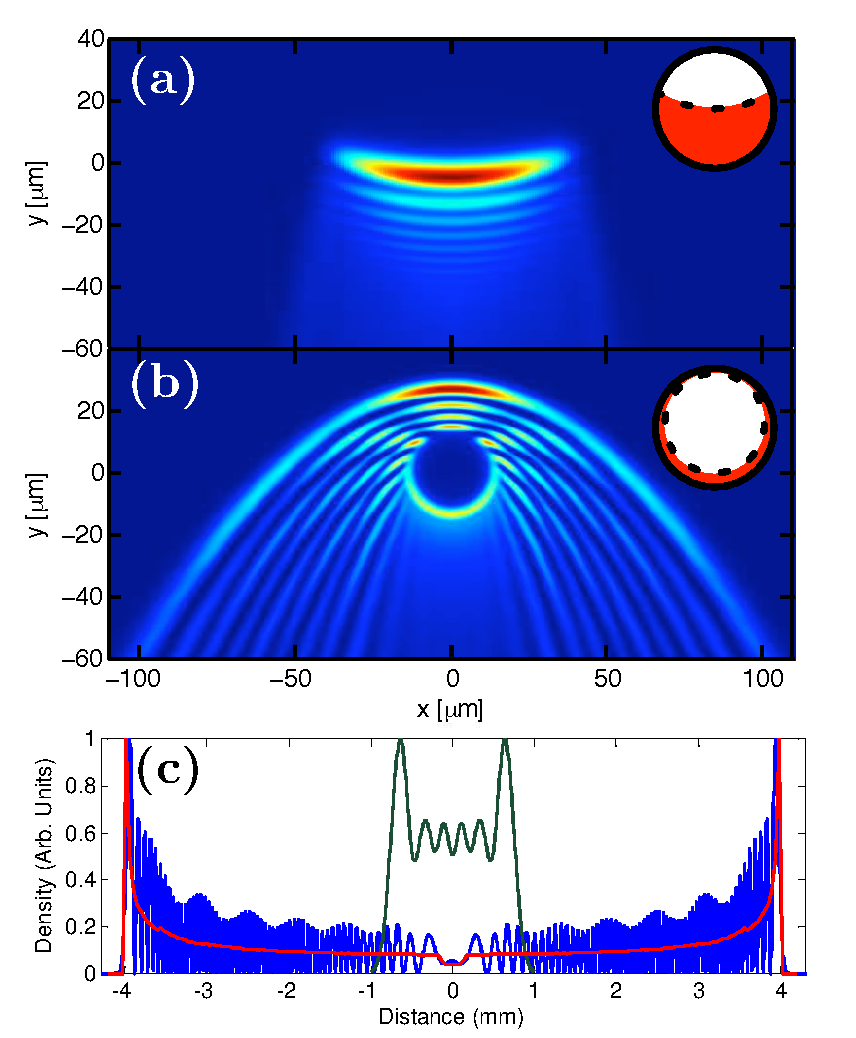
\includegraphics[width=10cm]{HeliumTransverseProfile}
    \caption{Near-field simulations of atom laser profiles, showing vastly different output dynamics depending whether output-coupling takes place on (a) planes or on (b) prolate spheroids.  The output-coupling regions (dashed line), relative to the BEC (circle), used to create these plots are shown diagrammatically in the upper right corner of each plot.  In both cases the BEC is located at the origin, with radial trapping frequencies of $\omega_r = 2 \pi \times \unit[50]{Hz}$ and $\omega_r = 2 \pi \times \unit[460]{Hz}$ respectively.  The resulting far field atom laser profiles as calculated at a detector $y=\unit[4]{cm}$ below the condensate for (a) and (b) are shown in (c).  The green profile results from the near field distribution shown in (a).  The blue and red profiles result from the near field distribution shown in (b) and are calculated using the Gross-Pitaevskii equation and classical mechanics respectively.  The classical simulation treats atoms as classical particles that begin on the outcoupling surface and are pushed from the BEC due to gravity and the mean field repulsion; the resulting `two-peak' structure is clearly visible.}
    \label{BackgroundTheory:HeliumTransverseProfile}
\end{figure}

It can be seen from the images of the near-field atom laser density in \figureref{BackgroundTheory:HeliumTransverseProfile}(a, b) that the transverse profile of the atom laser has significantly greater structure in the case of outcoupling from a tight trap than from a weak trap. This difference is quite dramatic in the far field as shown in \figureref{BackgroundTheory:HeliumTransverseProfile}(c), although the atom laser produced from a weak trap also has some interference fringes.  These interference fringes arise because it is possible for atoms outcoupled from different positions to have the same transverse momentum after leaving the condensate.  A large distance below the condensate these two atoms will occupy the same position and will interfere.  There are fewer interference fringes in the case of outcoupling from a weak trap as both atoms are accelerated downwards initially and therefore their maximum path length difference (and their maximum phase difference) will be smaller than if the atoms were outcoupled from a tight trap.  In the case of outcoupling from a tight trap, an atom that was initially accelerated upwards can have the same transverse momentum as an atom that was initially accelerated downwards.  The significantly larger maximum path length difference (and maximum phase difference) between these two atoms results in there being a greater number of interference fringes, as each $2\pi$ in the maximum phase difference corresponds to an interference fringe.  The maximum phase difference between two atoms arriving at the same location will vary from this maximum phase difference to zero.

While the fine structure of the transverse atom laser profile is caused by interference effects, the gross `double-peaked' structure is well-described classically [compare the red and blue lines of \figureref{BackgroundTheory:HeliumTransverseProfile}(c)].  The two peaks arise from the fact that, considered as a function of position on the outcoupling surface, there is a local maximum in the transverse momentum of the outcoupled atoms.  In the neighbourhood of this local maximum, the transverse momentum of outcoupled atoms will be approximately constant and therefore a greater number of atoms will contribute to the position on the detector corresponding to the maximum transverse momentum.  The `dip' in the centre of the transverse atom laser profile results from atoms which are outcoupled near the top of the outcoupling surface.  These atoms are initially accelerated upwards, but then fall back through the condensate.  This creates a shadowed region cast by the condensate, since atoms attempting to pass back through the condensate are pushed off axis due to the mean field repulsion.  This shadowed region is clearly visible below the condensate in \figureref{BackgroundTheory:HeliumTransverseProfile}(b).

\begin{figure}
    \centering
    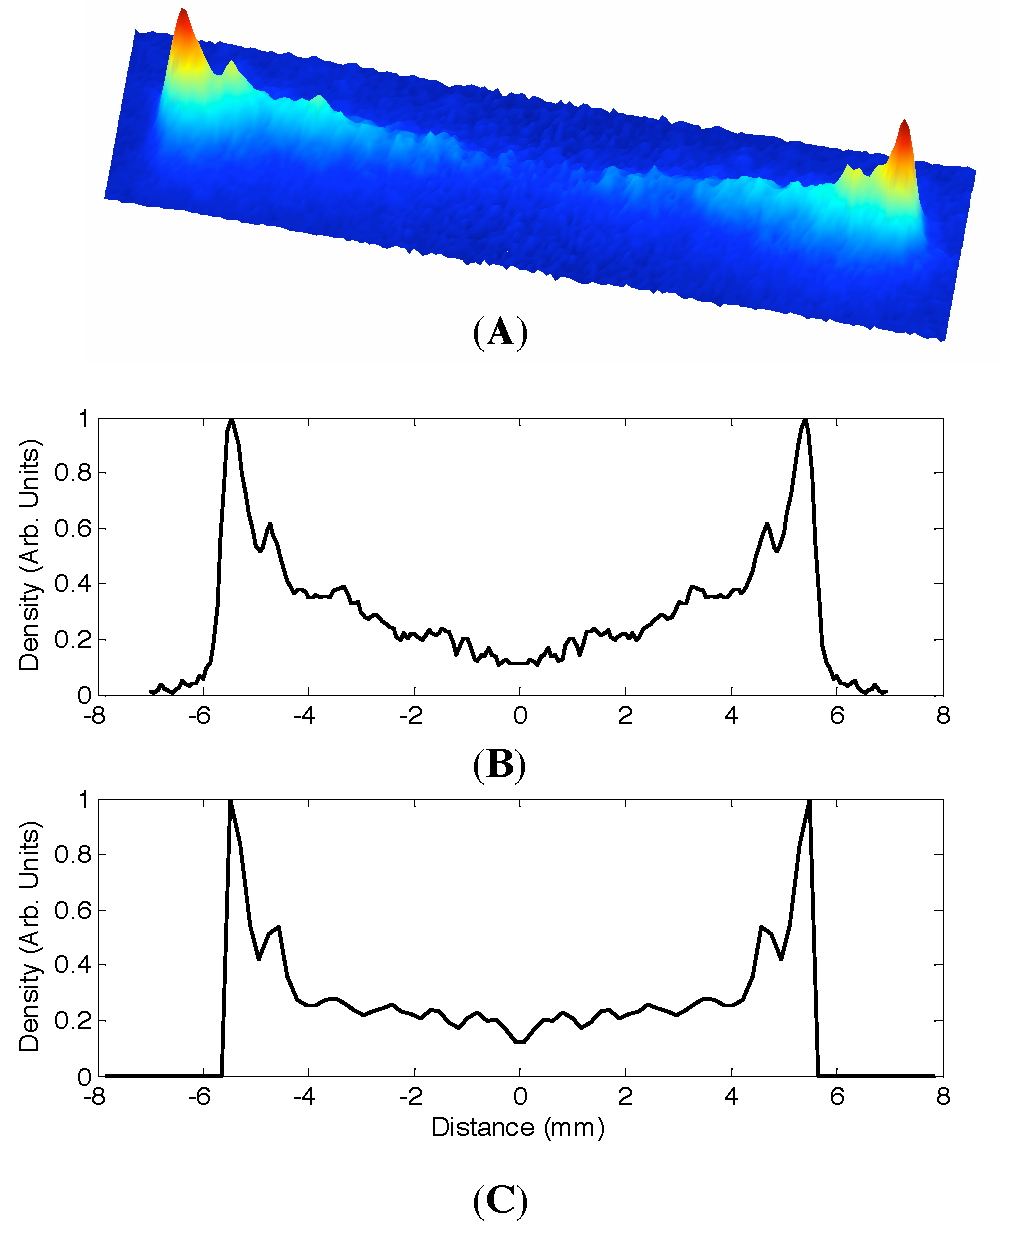
\includegraphics[width=10cm]{HeliumTransverseProfileExpTheoryComparison}
    \caption{Comparison of theory and experiment.  Upper trace shows an experimental 2D MCP image of the transverse profile of an atom laser (image size is $\unit[13]{mm}$ by $\unit[3.4]{mm}$).  Middle trace is an averaged profile taken through the centre of the 2D image.  Lower trace is the theoretical profile corresponding to the experimental conditions averaged over the detector resolution.}
    \label{BackgroundTheory:HeliumTransverseProfileExpTheoryComparison}
\end{figure}

\figureref{BackgroundTheory:HeliumTransverseProfileExpTheoryComparison} demonstrates that the results predicted by the Gross-Pitaevskii model of \eqref{BackgroundTheory:AtomLaserF1} are in good agreement with the experimental results from the ANU He* experiment \citep{Dall:2007}.  The atom laser profile shown is for the case of outcoupling with Rabi frequency $\Omega = 2\pi\times \unit[500]{Hz}$ from the centre of a condensate of $N=2 \times 10^6$ atoms held in a magnetic trap with trapping frequencies $\omega_r = 2\pi \times \unit[50]{Hz}$ and $\omega_z = 2 \pi \times \unit[460]{Hz}$.  While the form of Eqs.~\eqref{BackgroundTheory:AtomLaserF1} is not particularly complicated, their solution can be numerically intensive.  Producing the theoretical profile of \figureref{BackgroundTheory:HeliumTransverseProfileExpTheoryComparison} required first solving \eqref{BackgroundTheory:AtomLaserF1} for the steady-state of the atom laser in the region near the condensate.  This  required 2000 hours of CPU time on a supercomputer, significantly longer than the simulations depicted in \figureref{BackgroundTheory:HeliumTransverseProfile}.  The reason for this difference is that in the case of \figureref{BackgroundTheory:HeliumTransverseProfileExpTheoryComparison}, atoms were outcoupled from the centre of the condensate, and therefore the atoms were moving faster and travelled higher after leaving the condensate.  This necessitated the use of a much finer grid to resolve the spatial oscillations of the atom laser on the length scale of the de Broglie wavelength, and a much larger grid to accommodate the atoms that travelled higher.  Some of the numerical techniques used in simulations performed as part of this thesis are discussed in \sectionref{BackgroundTheory:NumericalTechniques}.

Although good agreement is seen between the predictions of the Gross-Pitaevskii model and the observed experimental profile, the presence of interference fringes on the atom laser will cause problems in mode matching the atom laser beam to another atom laser, as would be necessary in an atom interferometry experiment.  \figureref{BackgroundTheory:HeliumTransverseProfile} demonstrates that outcoupling from a weaker trap improves the transverse profile, making it closer to an ideal Gaussian beam.  It is also possible to improve the transverse mode by outcoupling closer to the bottom of the trap \citep{Riou:2006fk}, however this comes at the cost of reduced flux and a higher sensitivity to technical noise in the frequency of the outcoupling radiation \citep{Robins:2005uq}.  Other options for improving the transverse profile include using a multiphoton Raman outcoupling process \citep{Hagley:1999dz,Ruostekoski:2003,Jeppesen:2008} or guiding the atom laser optically \citep{Guerin:2006mz,Couvert:2008,Dall:2010}.  This last possibility, however, may introduce sufficient noise due to fluctuations in the waveguide to preclude its use in atom interferometry measurements \citep{Le-Coq:2006}.

\section{Loss processes and the master equation}

We are not always interested in the entirety of an interacting system; frequently it is only a small part of that system that is of interest.  For example, in \sectionref{BackgroundTheory:GrossPitaevskiiEquation} we considered a BEC and its environment of the almost empty atomic modes of the vacuum chamber in which it was produced.  The environment is vastly larger than the BEC, both in terms of the number of available atomic modes, and also in terms of the total occupation of those modes.  Condensates containing as many as $10^8$ \nucl{87}{Rb} atoms have been produced, however many more atoms ($\sim 10^{10}$) were initially in the trap before the evaporation process \citep{Streed:2006}.  The remaining atoms that are not part of the condensate comprise the environment.  While the entire system may be described by a many-body wavefunction, much of the information in this wavefunction will be describing the environment.  A description is necessary of the state of the condensate independent of the exact state of the environment.  The density matrix $\hat{\rho}$ provides that description \citep{Scully}.

As mentioned in \sectionref{BackgroundTheory:GrossPitaevskiiEquation}, a density matrix for a subsystem may be obtained by formally averaging (or tracing) over the degrees of freedom of the environment.  This simpler description fully describes the subsystem when we are restricted to performing measurements on the subsystem of interest.  With this very natural restriction it becomes impossible to distinguish otherwise distinct states of the entire system.  This indistinguishability is not fundamental; by performing measurements on the entire system the states may be distinguished.  The indistinguishability arises only due to our limited knowledge of the subsystem.

Although not part of the subsystem of interest, the environment typically still influences the evolution of the subsystem.  For example collisions with atoms in the environment will lead to losses from the condensate.  While knowledge of the state of the entire system is necessary to treat this exactly, if the interaction between the subsystem and its environment is sufficiently weak and the subsystem is sufficiently small in comparison to its environment, the interaction may be treated perturbatively using the master equation technique originally derived in the context of quantum optics \citep{Senitzky:1960,Senitzky:1961}.  Specifically, for subsystem--environment interactions of the form
\begin{align}
    \hat{H}_\text{int} &= \hbar \sum_m \left(\hat{X}_m^\dagger \hat{\Gamma}_m^{\phantom{\dagger}} + \hat{X}_m^{\phantom{\dagger}} \hat{\Gamma}_m^\dagger \right), \label{BackgroundTheory:GeneralSubsystemEnvironmentCoupling}
\end{align}
where $\{\hat{X}_m\}$ are a set of bosonic subsystem annihilation operators, and $\{\hat{\Gamma}_m\}$ are a set of bosonic environment annihilation operators, the equation of motion for the density matrix gains the following term \citep[Chapter 5]{GardinerQN}:
\begin{align}
    \left.\frac{\partial}{\partial t} \hat{\rho}\right|_\text{int} &= \sum_m K_m \mathcal{D}[\hat{X}_m]\hat{\rho} + \sum_m G_m \mathcal{D}[\hat{X}_m^\dagger]\hat{\rho}, \label{BackgroundTheory:LindbladForm}
\end{align}
where $\mathcal{D}[\hat{a}]\hat{\rho} = \hat{a} \hat{\rho} \hat{a}^\dagger - \frac{1}{2}\left(\hat{a}^\dagger \hat{a} \hat{\rho} + \hat{\rho} \hat{a}^\dagger \hat{a} \right)$ is the decoherence superoperator, and the positive constants $K_m$ and $G_m$ depend on properties of the environment.  In the common case that the environment operators $\hat{\Gamma}_m$ are products of annihilation operators, the constants $G_m$ are zero if the modes of the environment are essentially unoccupied.

In the following section the master equation will be used to model the process of Penning ionisation in metastable helium.

% A practical application of \eqref{BackgroundTheory:LindbladForm} is to the process of spontaneous emission.  Consider the case of a field of two-level atoms coupled by light.  Within certain approximations (see \sectionref{OpticalPumping:MultimodeModel} for details) the interaction Hamiltonian takes the form
% \begin{align}
%     \hat{H}_\text{int} &= \hbar \epsilon \int d \vect{x}\, \left(\hat{\Psi}_e^\dagger(\vect{x}) \hat{\Psi}_g^{\phantom{\dagger}}(\vect{x}) \hat{\Phi}_\text{ph}^{\phantom{\dagger}}(\vect{x}) + \hat{\Phi}_\text{ph}^\dagger(\vect{x}) \hat{\Psi}_g^\dagger(\vect{x}) \hat{\Psi}_e^{\phantom{\dagger}}(\vect{x})\right),
% \end{align}
% where $\epsilon$ is a coupling constant, $\hat{\Psi}_g$ and $\hat{\Psi}_e$ are the atomic field operators for the ground and excited states respectively, and $\hat{\Phi}_\text{ph}$ is the photon field operator.  If we are only interested in the behaviour of atoms in the excited state, we may consider $\hat{\Psi}_e$ to be our subsystem of interest with $\hat{\Psi}_g$ and $\hat{\Phi}_\text{ph}$ comprising the environment.  In this case, the subsystem operator $\hat{X}_m$ is $\hat{\Psi}_e$ and the environment operator $\hat{\Gamma}_m$ is $\hat{\Psi}_g \hat{\Phi}_\text{ph}$.  

\subsection{Application: Penning ionisation}
\label{BackgroundTheory:PenningIonisation}

The primary attraction of creating Bose-Einstein condensates of metastable helium atoms is that their large internal energy ($\unit[20]{eV}$) enables single-atom detection with high spatial (\micro m) and temporal resolution (ns). However, this large internal energy can be released when two metastable helium atoms collide, resulting in Penning ionisation (PI),
\begin{align}
    \label{BackgroundTheory:PenningIonisation}
    \text{He}^* + \text{He}^* & \rightarrow \left\{
        \begin{matrix}
            \text{He}^+ + \text{He} + e^-\\
            \text{He}_2^+ + e^-
        \end{matrix}\right..
\end{align}
While this process dominates for unpolarised cold samples such as magneto-optical traps~\citep{Bardou:1992}, it does not prohibit the formation of Bose-Einstein condensates as the process is suppressed by five orders of magnitude~\citep{Shlyapnikov:1994} in polarised samples.  This suppression is due to conservation of angular momentum. While the reactants each have a total angular momentum $s=1$, giving their combined total angular momentum as either $S=0$ or $S=2$ (assuming $s$-wave collisions), the products each have total angular momentum $s=\frac{1}{2}$ (in the case of $\text{He}^+$, $e^-$ and $\text{He}_2^+$) or $s=0$ (for $\text{He}$), giving the total angular momentum of the products as either $S=0$ or $S=1$. Hence spin polarised states having $S=2$, $m_S=\pm2$ cannot directly undergo the process \eqref{BackgroundTheory:PenningIonisation}.

In general as $S$ is conserved, any of the $S=2$ quasimolecule states will be prevented from directly undergoing PI. As collisions with nonzero relative angular momentum can be neglected at BEC temperatures~\citep{Venturi:2000,Stas:2006kx} (due to the atoms having insufficient energy to penetrate the centrifugal barrier), it is only the $S=0$ quasimolecule state that undergoes PI.

The Hamiltonian describing either of the processes \eqref{BackgroundTheory:PenningIonisation} will be of the form
\begin{align}
    \hat{H}_\text{int} &= \hbar \epsilon \int d \vect{x}\, \left(\hat{\Gamma}^\dagger(\vect{x})\hat{\Xi}_{S=0, m_S=0}^{\phantom{\dagger}}(\vect{x}) + \hat{\Xi}_{S=0, m_S=0}^\dagger (\vect{x}) \hat{\Gamma}(\vect{x}) \right), \label{BackgroundTheory:PIInteractionHamiltonian}
\end{align}
where $\epsilon$ is a spatially-independent coupling constant, $\hat{\Gamma}$ is a product of annihilation operators for the products of the PI process, and the $S=0$ quasimolecule state that undergoes PI is given by
\begin{align}
    \hat{\Xi}_{S=0, m_S=0} &= \frac{1}{\sqrt{3}} \left( 2 \hat{\Psi}_1 \hat{\Psi}_{-1} - \hat{\Psi}_0 \hat{\Psi}_0\right).
\end{align}

As we are only interested in the metastable helium atoms, and not the products of the PI process, $\hat{\Xi}_{S=0, m_S=0}$ is the subsystem operator of the interaction Hamiltonian \eqref{BackgroundTheory:PIInteractionHamiltonian}, and $\hat{\Gamma}$ is the environment operator.  As the environment operator is of the form of a product of annihilation operators and the products of PI will have sufficient kinetic energy to leave the condensate rapidly (and therefore keep the $\hat{\Gamma}$ modes near the condensate unoccupied), the master equation term describing Penning ionisation must have the form
\begin{align}
    \left.\frac{d \hat{\rho}}{dt}\right|_\text{PI} &= \gamma_\text{PI} \int d \vect{x}\, \mathcal{D}\left[ \hat{\Xi}_{S=0, m_S=0}\right] \hat{\rho}, \label{BackgroundTheory:PenningIonisationMasterEquationTerm}
\end{align}
where $\gamma_\text{PI}$ is a positive rate constant.  An explicit form for this rate constant is obtained in \sectionref{PenningIonisationAppendix:MasterEquation}.  It is shown there that $\gamma_\text{PI} = \frac{9}{2} \Kunpol$, where $\Kunpol = \unit[7.7\times 10^{-17}]{m\textsuperscript{3}s\textsuperscript{-1}}$ is the rate constant for the production of ions due to Penning ionisation in an unpolarised thermal sample at $\unit[1]{\micro K}$~\citep{Stas:2006kx}.

\section{Beyond the Gross-Pitaevskii equation}
\label{BackgroundTheory:BeyondGrossPitaevskii}

In deriving the Gross-Pitaevskii equation, the atomic field $\hat{\Psi}(\vect{x})$ was separated into a classical component $\Psi(\vect{x})$ and a fluctuations operator $\delta\hat{\Psi}(\vect{x})$,
\begin{align}
    \hat{\Psi}(\vect{x}) &= \Psi(\vect{x}) + \delta\hat{\Psi}(\vect{x}),
\end{align}
where it was then assumed that the fluctuations operator was `small'.  This is the so-called semiclassical or mean-field approximation which includes single-particle quantum mechanical effects such as interference and barrier-tunnelling.  This approximation neglects some of the more interesting quantum phenomena such as entanglement and squeezing \citep{Scully}.  This section discusses some techniques beyond the Gross-Pitaevskii equation that include these quantum statistical effects to varying levels of approximation.  

There are two classes of methods that go beyond semiclassical approximations.  In the first class of methods the state of the system is quite general and an expansion is performed in the evolution of the system, which is truncated at a certain level.  The stochastic phase-space methods are the most common of this class, and are discussed in  \sectionref{BackgroundTheory:StochasticPhaseSpaceMethods}.  In the second class of methods, an expansion is performed in the form of the system's state.  This expansion is truncated at some level, neglecting correlations above a certain order.  Requiring the state of the system to be of a certain form implicitly approximates the evolution of the system as well, however these approximations are of a different kind to those of the first class.  The Bogoliubov-type methods are representative of the second class of methods, and are discussed in \sectionref{BackgroundTheory:BogoliubovMethods}.

% Note that Karen's recent +P / HFB (bog?) hybrid is a cross-over between these two classes.


\subsection{Stochastic phase-space methods}
\label{BackgroundTheory:StochasticPhaseSpaceMethods}

% c-number methods?

Phase-space representations are real-valued functions that are an alternative description of the state of the system, fully equivalent to the density matrix $\hat{\rho}$.  In addition to being useful pictorial representations of the state of a system, these phase-space representations can be used to derive stochastic methods for describing the evolution of the system.

There are several phase-space representations, the most common being the P, Q and Wigner distributions.  Each of these represent the state of the system in terms of coherent states.  This is mostly clearly seen for the P-function,
\begin{align}
    \hat{\rho} &= \int d \alpha\, P(\alpha) \ketbra{\alpha}{\alpha}, \label{BackgroundTheory:PFunction}
\end{align}
where $P(\alpha)$ is the P-function for the single-mode system described by the density matrix $\hat{\rho}$.  Every density matrix has a unique P-function representation.  This P-function representation fully describes the state of the system and is completely equivalent to the density matrix itself.  

While the P-function is real, it is frequently pathological.  For example, the coherent state $\ket{\alpha_0}$ has the P-function representation
\begin{align}
    P(\alpha) &= \delta^2(\alpha - \alpha_0).
\end{align}
The Wigner and Q functions are significantly less pathological as they can be obtained by convolving the P-function with $\frac{2}{\pi}e^{-2 \abs{\alpha}^2}$ and $\frac{1}{\pi} e^{-\abs{\alpha}^2}$ respectively.  Despite this convolution, the Wigner and Q functions are also complete representations of the state of the system \citep{GardinerQN}.

Instead of considering the evolution of the density matrix directly, the stochastic phase-space methods aim to model the evolution of phase-space representations.  If the equation of motion for the phase-space representation is of the form of a Fokker-Planck equation \citep{GardinerHSM}, the phase-space representation may be interpreted as a classical probability distribution.  In this case the evolution may be unravelled using stochastic differential equations.  Expectation values can then be calculated as averages of appropriate quantities over \emph{independent} realisations of a stochastic differential equation, which requires significantly fewer computational resources than solving the Fokker-Planck equation directly.  

In the general case it is desired to unravel the Fokker-Planck equation
\begin{align}
    \frac{\partial}{\partial t}F(\vect{\alpha}, t) &= - \sum_j \frac{\partial}{\partial \alpha_j} A_j(\vect{\alpha}, t) F(\vect{\alpha}, t) + \frac{1}{2} \sum_{j, k} \frac{\partial}{\partial \alpha_j^{\phantom{*}}} \frac{\partial}{\partial \alpha_k^*} D_{j,k}(\vect{\alpha}, t) F(\vect{\alpha}, t) \label{BackgroundTheory:GeneralFokkerPlanckEquation}
\end{align}
in terms of the Stratonovich stochastic differential equation \citep{GardinerHSM}
\begin{align}
    d \alpha_i &= A_i(\vect{\alpha}, t)\, dt  - \frac{1}{2} \sum_{j, k} B_{k, j}(\vect{\alpha}, t) \frac{\partial }{\partial \alpha_k}B_{i,j}(\vect{\alpha}, t) \, dt + \sum_j B_{i,j}(\vect{\alpha}, t) \,d W_j(t), \label{BackgroundTheory:GeneralStratonovichSDE}
\end{align}
where the matrix $\vect{B}(\vect{\alpha}, t)$ is defined by
\begin{align}
    \vect{D}(\vect{\alpha}, t) &= \vect{B}(\vect{\alpha}, t) \vect{B}^\dagger(\vect{\alpha}, t),
\end{align}
and the Wiener increments $d W_j(t)$ are independent real Gaussian random variables with zero mean satisfying
\begin{align}
    \overline{d W_i(t) dW_j(t')} = \delta_{i j}\delta(t - t'),
\end{align}
where $\overline{(\cdot)}$ denotes an average over the random variables.  This decomposition is guaranteed when the matrix $\vect{D}(\vect{\alpha}, t)$ has only positive eigenvalues~\citep{GardinerHSM}, and may be possible when this requirement is loosened to only nonnegative eigenvalues. Note that the sums in \eqref{BackgroundTheory:GeneralFokkerPlanckEquation} and \eqref{BackgroundTheory:GeneralStratonovichSDE} are defined to run over both the complex variables $\alpha_j^{\phantom{*}}$ and their conjugates $\alpha_j^*$.

The unravelling of a Fokker-Planck equation in terms of a stochastic differential equation can be physically interpreted as the macroscopic and microscopic views of the same process. For example, a Fokker-Planck equation can be used to model the probability distribution of positions and velocities of particles in a gas (macroscopic view), and the corresponding stochastic differential equation would describe the path taken by a single particle (microscopic view).  The macroscopic view is useful when it is the distribution of positions and velocities which is of interest, or if it is only a few moments that are of interest, when the equations of motion for those moments form a closed system (such as those describing an ideal gas). Frequently however the equations of motion are not closed with that for each moment depending on a higher-order moment [for example \eqref{BackgroundTheory:ExpectationValueEvolution}], and an assumption must be made to close the system of equations (in the case of \eqref{BackgroundTheory:ExpectationValueEvolution}, that the system remains in a coherent state). 

The microscopic view is an alternative approach which is useful when two conditions are met. The first is that it is only a finite set of moments of the distribution that are of interest, not the distribution itself. The second is that the motion of the particles are independent of one another (although they may depend on moments of the distribution). That the particles' motions are independent is equivalent to the eigenvalues of $\vect{D}(\vect{\alpha}, t)$ being nonnegative. Positive eigenvalues of $\vect{D}(\vect{\alpha}, t)$ can be physically interpreted as corresponding to a diffusion process which microscopically takes the form of Brownian motion. Negative eigenvalues however correspond to \emph{negative} diffusion, a highly singular process in which particles tend to drift toward one another\footnote{It should be noted that the existence of negative eigenvalues for the matrix $\vect{D}(\vect{\alpha}, t)$ does not imply that the \emph{solution} to the Fokker-Planck equation is singular. A good example of this is the equation of motion for the Q function~\citep{Scully} of the anharmonic oscillator which is periodic in time, yet the corresponding $\vect{D}(\vect{\alpha}, t)$ matrix has positive and negative eigenvalues of equal magnitude.}.  In this case the evolution of one realisation of \eqref{BackgroundTheory:GeneralStratonovichSDE} will depend on the local \emph{distribution}, violating the conditions stated above.  One solution to this problem is increase the dimensionality of the Fokker-Planck equation and use the additional freedom given by the auxiliary dimensions to ensure that motion in the larger space is purely diffusive (this approach is taken with the Positive-P representation~\citep{GardinerQN}).  While this technique is exact in the limit of an infinite number of realisations of the corresponding stochastic differential equation, it is typically limited by the existence of trajectories with arbitrarily large norm \citep{Gilchrist:1997fk}.  These trajectories increase the sampling error in calculated observables.  This problem is particularly acute for BEC systems as the atomic scattering process described by \eqref{BackgroundTheory:SimpleScattering} causes the stochastic sampling error to diverge exponentially \citep{Gilchrist:1997fk}.  Such doubled phase-space techniques can therefore only describe the evolution of the system for short times.

% The Fokker-Planck equation is a faster technique when it is the distribution that is of interest, however the stochastic unravelling is a faster technique when it is only a few moments that are of interest.

\subsubsection{Application: Anharmonic oscillator}

We now demonstrate the application of a stochastic phase-space method to the anharmonic oscillator, which is governed by the Hamiltonian
\begin{align}
    \hat{H} = \hbar \omega \hat{a}^\dagger \hat{a} + \frac{1}{2} \hbar \kappa \hat{a}^\dagger \hat{a}^\dagger \hat{a} \hat{a}. \label{BackgroundTheory:AnharmonicOscillator:Hamiltonian}
\end{align}
We wish to consider the evolution of the system with initial state $\ket{\Psi(0)} = \ket{\alpha_0}$.  This system can be solved exactly and has the interesting feature that its two-time correlation function initially decays, but undergoes perfect revivals when $\kappa t = 2 \pi n$ for integral $n$.  The normalised two-time correlation function for this system is
\begin{align}
    \frac{1}{N}\abs{\mean{\hat{a}^\dagger(t) \hat{a}(0)}}^2 &= \exp \left\{2 N \left[\cos(\kappa t) - 1 \right] \right\}, \label{BackgroundTheory:AnharmonicOscillator:ExactTwoTimeCorrelationFunction}
\end{align}
where $N = \abs{\alpha_0}^2$.

In this thesis we will only consider stochastic methods based on the Wigner distribution, which is defined by \citep{Scully}
\begin{align}
    W(\alpha) &= \frac{1}{\pi^2} \int d^2 \lambda\, \exp\left(-\lambda \alpha^* + \lambda^* \alpha\right) \Tr\left\{ \exp\left(\lambda \hat{a}^\dagger - \lambda^* \hat{a}\right) \hat{\rho} \right\}.
\end{align}
An equation of motion for the Wigner function can be obtained using the equation of motion for the density matrix:
\begin{align}
    \frac{\partial}{\partial t} W(\alpha) &= \frac{1}{\pi^2} \int d^2 \lambda\, \exp\left(-\lambda \alpha^* + \lambda^* \alpha\right) \Tr\left\{ \exp\left(\lambda \hat{a}^\dagger - \lambda^* \hat{a}\right) \frac{\partial}{\partial t}\hat{\rho}\right\} \notag \\
    &= \frac{1}{\pi^2} \int d^2 \lambda\, \exp\left(-\lambda \alpha^* + \lambda^* \alpha\right) \Tr\left\{ \exp\left(\lambda \hat{a}^\dagger - \lambda^* \hat{a}\right) \frac{-i}{\hbar} \left[\hat{H},\, \hat{\rho} \right]\right\},
\end{align}
for evolution driven by a Hamiltonian $\hat{H}$.  The simplification of this expression is made easier through the application of the following operator correspondences \citep[\S 4.5]{GardinerQN}
\begin{subequations}
    \begin{align}
        \hat{a} \hat{\rho} &\leftrightarrow \left(\alpha + \frac{1}{2} \frac{\partial}{\partial \alpha^*} \right) W(\alpha), \\
        \hat{\rho} \hat{a} & \leftrightarrow \left(\alpha - \frac{1}{2} \frac{\partial}{\partial \alpha^*} \right) W(\alpha), \\
        \hat{a}^\dagger \hat{\rho} & \leftrightarrow \left( \alpha^* - \frac{1}{2} \frac{\partial}{\partial \alpha} \right) W(\alpha), \\
        \hat{\rho} \hat{a}^\dagger & \leftrightarrow \left( \alpha^* + \frac{1}{2} \frac{\partial}{\partial \alpha} \right) W(\alpha).
    \end{align}
\end{subequations}
These correspondences apply for general density matrix evolution, not only for evolution driven purely by a Hamiltonian (see, for example \sectionref{PenningIonisationAppendix:TW}).

For the anharmonic oscillator Hamiltonian \eqref{BackgroundTheory:AnharmonicOscillator:Hamiltonian}, the evolution equation for the Wigner distribution is
\begin{align}
    \label{BackgroundTheory:AnharmonicOscillator:WignerEvolution}
    \begin{split}
        \frac{\partial}{\partial t} W(\alpha) &=  i\left( \frac{\partial}{\partial \alpha} \alpha - \frac{\partial}{\partial \alpha^*} \alpha^*\right) \left[\omega + \kappa\left(\abs{\alpha}^2 - 1\right) \right] W(\alpha)\\
        &-\frac{1}{4}i \kappa \left(\frac{\partial^2}{\partial \alpha^2}\frac{\partial}{\partial \alpha^*}\alpha - \frac{\partial^2}{\partial {\alpha^*}^2} \frac{\partial}{\partial \alpha} \alpha^*\right) W(\alpha).
    \end{split}
\end{align}
The third-order derivatives in this equation mean that it is not in the form of a Fokker-Planck equation [cf.\ \eqref{BackgroundTheory:GeneralFokkerPlanckEquation}], and therefore may not be unravelled in terms of stochastic differential equations.  However, if these higher-order derivatives are neglected the equation of motion will only contain first-order derivatives and may therefore be unravelled in terms of stochastic differential equations.  In fact, due to the absence of second-order derivatives, there will be no noise term in the resulting stochastic differential equations.  The initial condition for these equations is, however, stochastic. 

The neglect of third and higher-order derivatives in the equation of motion for the Wigner distribution is known as the Truncated Wigner (TW) approximation.  This is an uncontrolled approximation in the sense that there is no explicit small parameter in which this approximation is an expansion in.  We can motivate this approximation in the present system by considering the initial state of the Wigner distribution,
\begin{align}
    W(\alpha, t=0) &= \frac{2}{\pi} \exp\left(- 2 \abs{\alpha - \alpha_0}^2\right). \label{BackgroundTheory:WignerFunctionCoherentState}
\end{align}
As $\alpha_0$ changes, the initial Wigner distribution simply translates.  For small times therefore, each derivative can be considered to be of size $O(1)$.  The relative importance of each term in \eqref{BackgroundTheory:AnharmonicOscillator:WignerEvolution} therefore solely depends on the powers of $\alpha$ and $\alpha^*$.  The size of $\alpha$ and $\alpha^*$ can be considered to be of the order of $O(\alpha_0)$ as it is only in the vicinity of $\alpha_0$ that the Wigner distribution is significantly different from zero (for small times).  The first-order terms therefore scale as $O(\abs{\alpha_0}^2 \alpha_0)$, while the third-order terms scale as $O(\alpha_0)$.  For sufficiently large $\alpha_0$, the third-order derivatives in \eqref{BackgroundTheory:AnharmonicOscillator:WignerEvolution} can be neglected, at least for small times.  The accuracy of the Truncated Wigner approximation has been considered in great detail elsewhere \citep{Sinatra:2002lq,Norrie:2005fk,Norrie:2006vn,Norrie:2006kx,Polkovnikov:2003}.  In general it has been shown that it is a good approximation if the total occupation of the system is much greater than the number of available modes \citep{Norrie:2006vn}.  For the anharmonic oscillator, this requires $N = \abs{\alpha_0}^2 \gg 1$.

We continue now with the application of the Truncated Wigner method to the anharmonic oscillator.  With the third-order derivatives neglected, the Stratonovich stochastic differential equation describing the system is
\begin{align}
    d \alpha &= -i \left[\omega + \kappa \left(\abs{\alpha}^2 - 1\right) \right] \alpha \, dt. \label{BackgroundTheory:AnharmonicOscillator:SDE}
\end{align}
Although the evolution of this `stochastic' differential equation is deterministic, its initial condition is random as it must sample the initial condition of the Wigner distribution \eqref{BackgroundTheory:WignerFunctionCoherentState}.  The initial condition of \eqref{BackgroundTheory:AnharmonicOscillator:SDE} is therefore
\begin{align}
    \alpha(0) &= \alpha_0 + \frac{1}{\sqrt{2}} \eta,
\end{align}
where $\eta$ is a complex Gaussian random variable satisfying
\begin{align}
    \overline{\eta} &= 0, & \overline{\eta \eta} &= 0, & \overline{\eta^* \eta} &= 1.
\end{align}
The noise term in the initial state can be considered to be adding, on average, half a `virtual' particle per mode to the system \citep{Scott:2007}.  These virtual particles represent the contribution of the vacuum fluctuations that is ignored in the Gross-Pitaevskii equation.

In principle \eqref{BackgroundTheory:AnharmonicOscillator:SDE} can be simulated numerically to determine the dynamics of the system.  However, as it is of a particularly simple form it may be integrated analytically.  Within the Truncated Wigner approximation, the normalised two-time correlation function of the anharmonic oscillator is
\begin{align}
    \frac{1}{N} \abs{ \mean{\hat{a}^\dagger(t) \hat{a}(0)}_\text{TW}}^2 &= \frac{16}{(4 + \kappa^2 t^2)^2} \exp\left(\frac{- 4 N \kappa^2 t^2}{4 + \kappa^2 t^2} \right).
\end{align}
A comparison of the exact and truncated solutions is given in \figureref{BackgroundTheory:TwoTimeTWComparison}.

\begin{figure}
    \centering
    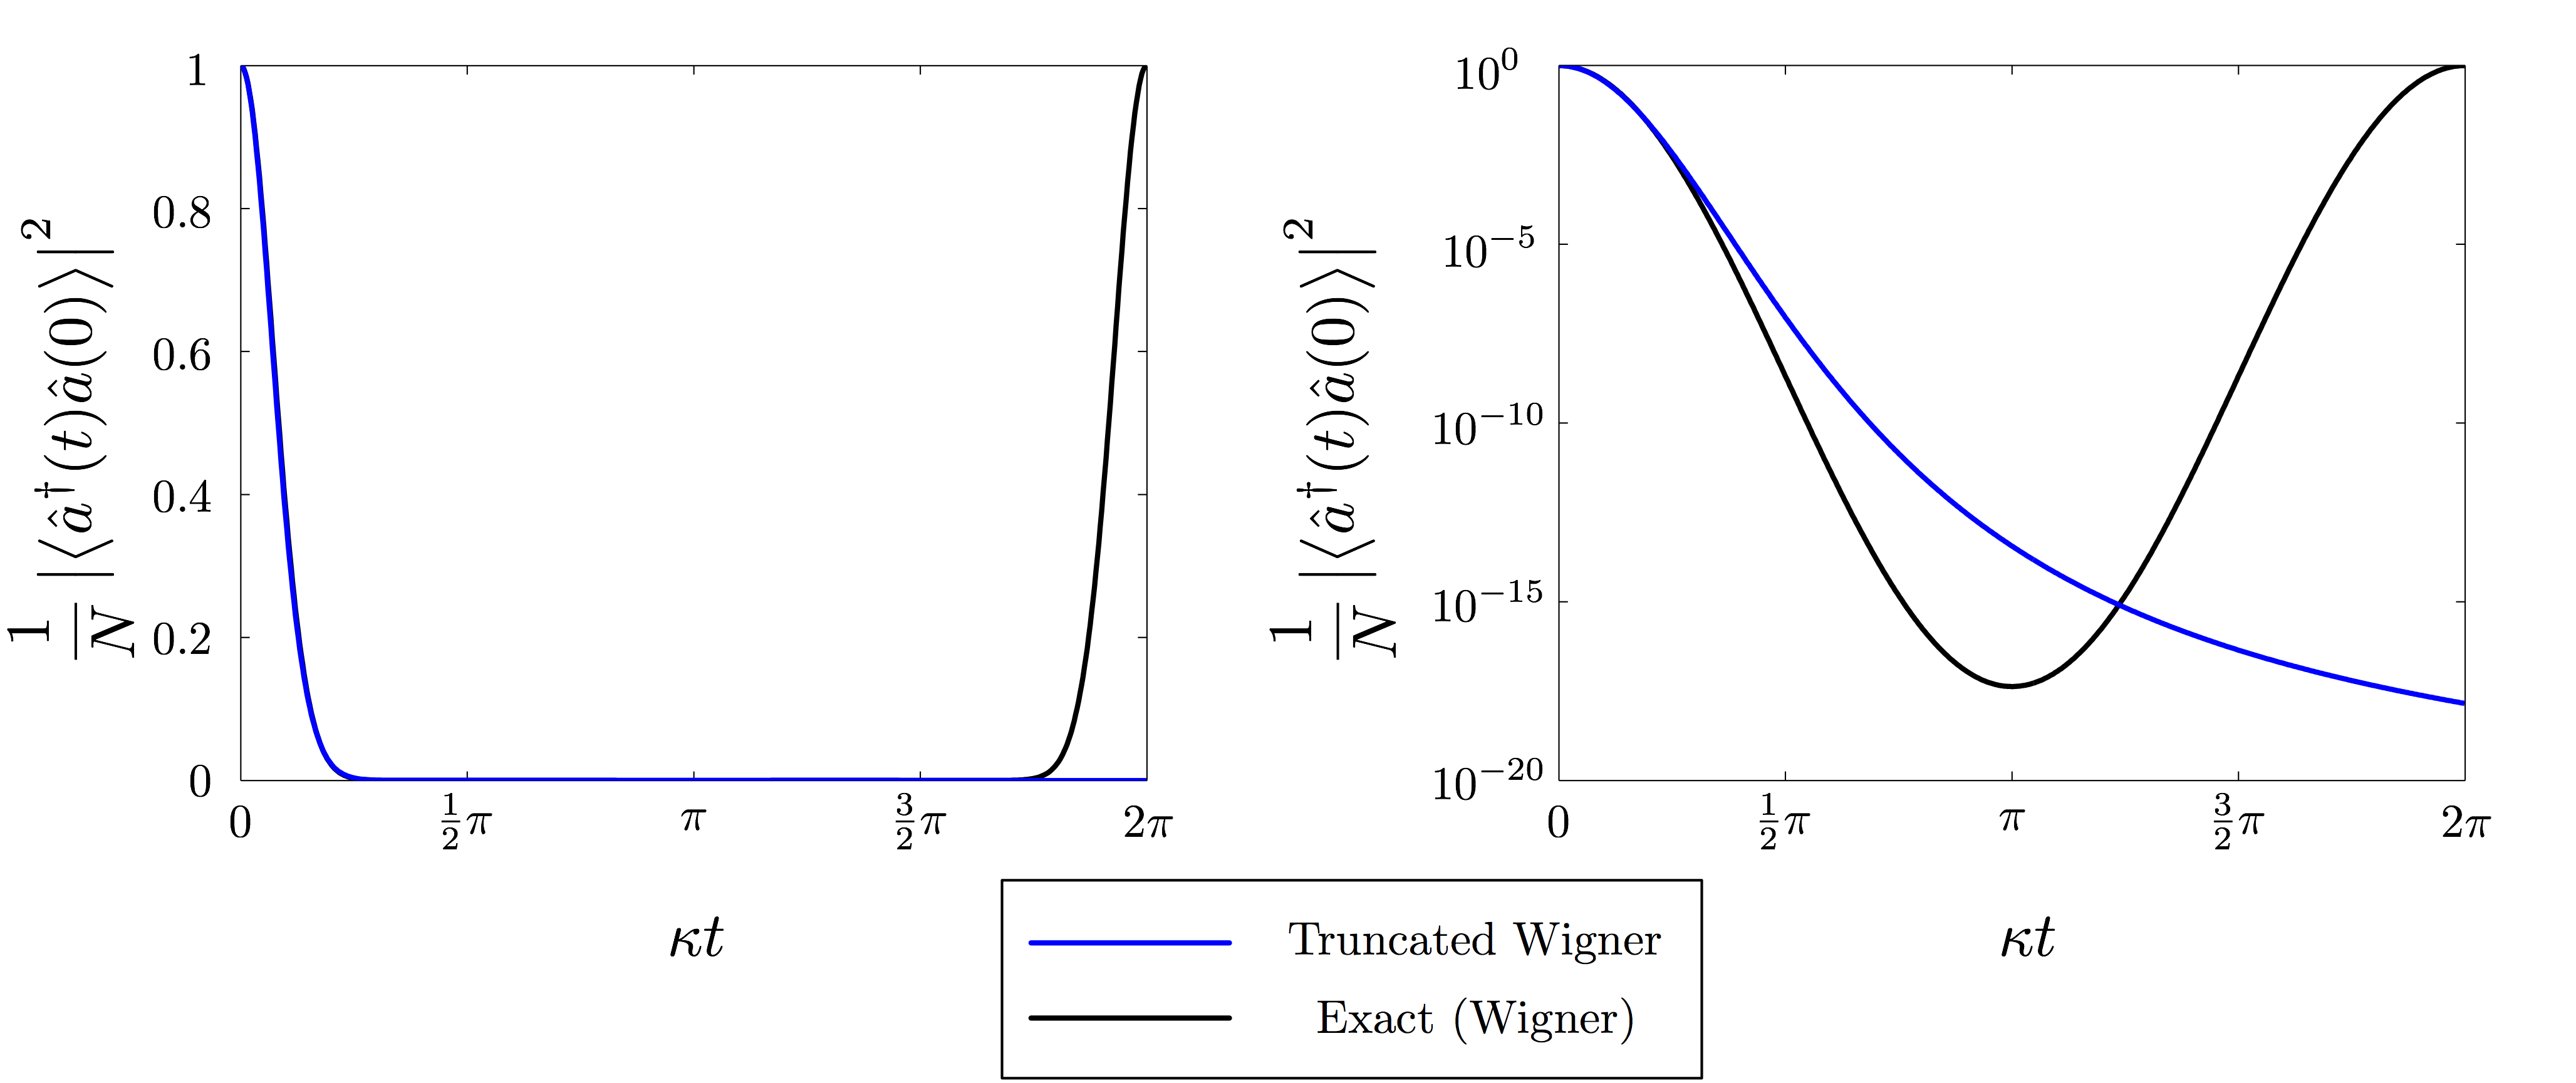
\includegraphics[width=15cm]{TwoTimeTWComparison}
    \caption{
        Comparison of Truncated Wigner with the exact solution for the two-time correlation function of the anharmonic oscillator.  The exact solution (black) for the two-time correlation function exhibits revivals every $\kappa t = 2\pi$, while the Truncated Wigner solution (blue) does not.  The Truncated Wigner solution, however, is in good agreement with the exact solution for the collapse of the correlation function.  The left and right figures illustrate the normalised two-time correlation function on linear and logarithmic scales respectively.  The initial condition was $\alpha_0 = \sqrt{10}$. \label{BackgroundTheory:TwoTimeTWComparison}
    }
\end{figure}

The good agreement between the Truncated Wigner and exact results in \figureref{BackgroundTheory:TwoTimeTWComparison} for $\kappa t \lesssim \frac{\pi}{4}$ does not imply that the distributions themselves are approximately equal over this time.  This is shown not to be the case in \figureref{BackgroundTheory:WignerTruncatedWignerComparison}, in which the Wigner and Truncated Wigner distributions for the anharmonic oscillator are compared.  Expectation values of higher-order moments will diverge from the exact solutions faster than those for lower-order moments.  The validity of Truncated Wigner therefore also depends on the moments that are to be calculated.  Typically, it is only second order moments such as $\mean{\hat{a}^\dagger \hat{a}}$ that are of interest. This is the case in this thesis.

\begin{figure}
    \centering
    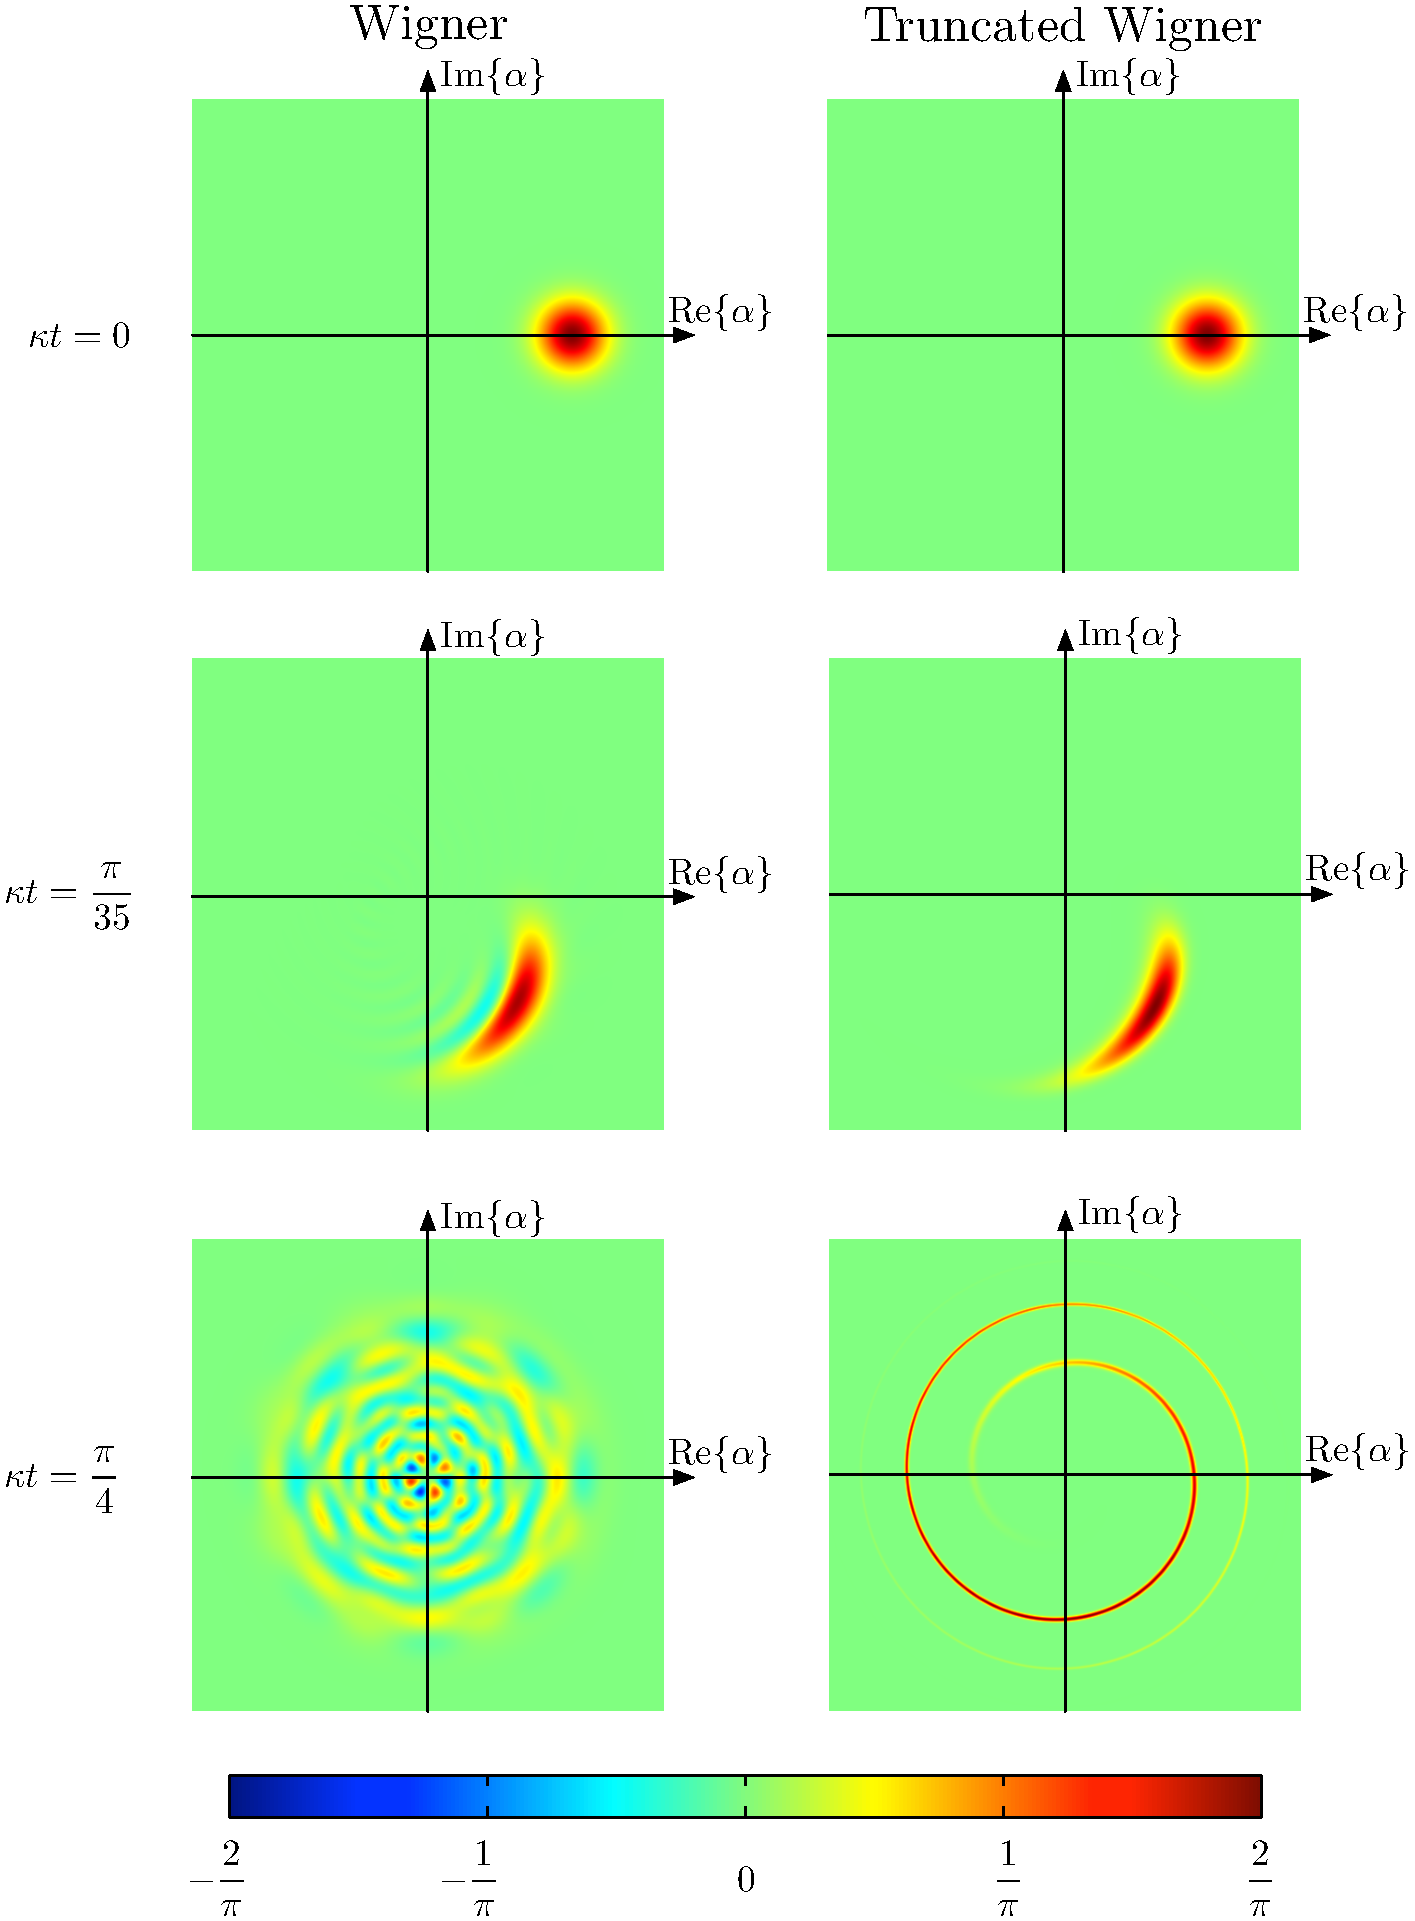
\includegraphics[width=14cm]{WignerTruncatedWignerComparison}
    \caption{
        Comparison of the Wigner and Truncated Wigner distributions for the anharmonic oscillator.  For short times, the two distributions are approximately equal (upper and middle rows), however for longer times (lower row) the Wigner distribution develops a significant negative components (blue).  As the Truncated Wigner distribution represents the probability distribution of the stochastic differential equation \eqref{BackgroundTheory:AnharmonicOscillator:SDE}, it remains positive.  The initial condition was $\alpha_0 = \sqrt{10}$. \label{BackgroundTheory:WignerTruncatedWignerComparison}
    }
\end{figure}

\parasep

Stochastic phase-space methods were described as being an expansion in the evolution of the system with no restriction on the state of the system.  The expansion in the evolution occurs at the level of the equation of motion for the phase-space distribution.  For an unravelling in terms of stochastic differential equations to be possible, all derivatives in this equation above second order must be truncated.  Although the requirement that the Truncated Wigner distribution be non-negative does impose a restriction on the state of the system, this restriction is not necessary \citep{Hush:2010}.  \citet{Polkovnikov:2003} has shown explicitly that the Gross-Pitaevskii equation and the Truncated Wigner method can be considered to be the zeroth and first order terms in an expansion of the system dynamics in terms of its response to quantum fluctuations.  In principle, higher-order corrections can be included, however the computational requirements increase rapidly for each additional correction considered.

Although the application of the Truncated Wigner method considered in this section did not involve explicitly stochastic evolution, an application that does is discussed in \appendixref{PenningIonisationAppendix}.

\subsection{Bogoliubov-type methods}
\label{BackgroundTheory:BogoliubovMethods}

The Bogoliubov-type methods consider the evolution of a truncated expansion of the state of the system.  These methods begin by decomposing the atomic field operator $\hat{\Psi}$ in terms of a classical component $\Psi = \mean{\hat{\Psi}}$ and a fluctuations operator $\delta \hat{\Psi}$,
\begin{align}
    \hat{\Psi} &= \Psi + \delta \hat{\Psi}.
\end{align}
The equations of motion for $\Psi$ and $\delta\hat{\Psi}$ may be obtained from \eqref{BackgroundTheory:ExpectationValueEvolution} and \eqref{BackgroundTheory:LocalOperatorEvolution} respectively \citep{Proukakis:2008},
\begin{subequations}
    \label{BackgroundTheory:Bogoliubov:GeneralEvolutionEquations}
    \begin{align}
        \begin{split}
            i \hbar \frac{\partial}{\partial t} \Psi &= \left(- \frac{\hbar^2 \nabla^2}{2 M} + V(\vect{x}) + U_\text{int} \abs{\Psi}^2 + 2 U_\text{int} \mean{\delta\hat{\Psi}^\dagger \delta\hat{\Psi}} \right) \Psi\\
            & + U_\text{int} \left(\mean{\delta\hat{\Psi} \delta\hat{\Psi}} \Psi^* + \mean{\delta\hat{\Psi}^\dagger \delta\hat{\Psi} \delta\hat{\Psi}} \right),
        \end{split} \label{BackgroundTheory:Bogoliubov:OrderParameterEvolution}\\
        \begin{split}
            i \hbar \frac{\partial}{\partial t} \delta\hat{\Psi} &= \left(-\frac{\hbar^2 \nabla^2}{2 M} + V(\vect{x}) + 2 U_\text{int} \abs{\Psi}^2 \right)\delta \hat{\Psi} + U_\text{int} \Psi^2 \delta \hat{\Psi}^\dagger\\
            &+ 2 U_\text{int} \Psi \left(\delta\hat{\Psi}^\dagger\delta\hat{\Psi} - \mean{\delta\hat{\Psi}^\dagger\delta\hat{\Psi}} \right)+ U_\text{int} \Psi^* \left(\delta \hat{\Psi}\delta \hat{\Psi} - \mean{\delta \hat{\Psi}\delta \hat{\Psi}} \right)\\
            &+ U_\text{int} \left(\delta\hat{\Psi}^\dagger \delta\hat{\Psi} \delta\hat{\Psi} - \mean{\delta\hat{\Psi}^\dagger \delta\hat{\Psi} \delta\hat{\Psi}} \right).
        \end{split} \label{BackgroundTheory:Bogoliubov:FluctuationOperatorEvolution}
    \end{align}
\end{subequations}
These equations are completely equivalent to the operator equation of motion \eqref{BackgroundTheory:LocalOperatorEvolution}, and are therefore equally infeasible to simulate numerically.  An approximation is needed to proceed.

There are a variety of methods that approximate \eqref{BackgroundTheory:Bogoliubov:GeneralEvolutionEquations} to varying degrees.  An extensive discussion of these methods is given in \citep{Proukakis:2008}.  The simplest of these is the Bogoliubov method in which the mean-field evolution \eqref{BackgroundTheory:Bogoliubov:OrderParameterEvolution} is approximated by the Gross-Pitaevskii equation and all terms of second- or higher-order in $\delta\hat{\Psi}$ are neglected.  This approximation restricts the applicability of this simplest method to the zero-temperature limit, where the contribution of the thermal cloud is small.  In this limit, however, the equations of motion are of sufficiently simple form as to enable analytic results to be obtained.  The Bogoliubov method is discussed in greater detail in \sectionref{Peaks:ElementaryExcitations}, and used in \sectionref{Peaks:PerturbativeApproach} to determine the stability of a He* condensate to excitations.

While the Bogoliubov method is useful in the zero-temperature limit, it does not consider effects such as scattering between the condensate and thermal fractions that are significant at higher temperatures.  In this limit more accurate methods based on \eqref{BackgroundTheory:Bogoliubov:GeneralEvolutionEquations} such as the Hartree-Fock and Hartree-Fock-Bogoliubov methods are necessary.  These methods expand the state in terms of moments of the fluctuation operator.  This expansion is typically truncated at second-order, with the state described (in the case of Hartree-Fock-Bogoliubov theory) in terms of the moments
\begin{align*}
    \Psi(\vect{x}) &= \mean{\hat{\Psi}(\vect{x})}, & G_N(\vect{x}, \vect{x}') &= \mean{\delta\hat{\Psi}^\dagger(\vect{x}') \delta\hat{\Psi}(\vect{x})}, & G_A(\vect{x}, \vect{x}') &= \mean{\delta\hat{\Psi}(\vect{x}') \delta\hat{\Psi}(\vect{x})}.
\end{align*}
All higher-order moments are approximately expressed in terms of lower-order moments using Wick's theorem \citep{Wick:1950,Blaizot:1986}.  For example
\begin{align}
    \mean{\delta\hat{\Psi}^\dagger \delta\hat{\Psi}^\dagger \delta\hat{\Psi} \delta\hat{\Psi}} &\approx 2 \mean{\delta\hat{\Psi}^\dagger \delta\hat{\Psi}} \mean{\delta\hat{\Psi}^\dagger \delta\hat{\Psi}} + \mean{\delta\hat{\Psi}^\dagger \delta\hat{\Psi}^\dagger} \mean{\delta\hat{\Psi} \delta\hat{\Psi}}.
\end{align}

While these methods are appropriate at intermediate temperatures, other techniques are necessary near the phase transition at $T\sim T_c$.  Methods appropriate in this limit are discussed in the following section.

\subsection{Methods applicable near the critical temperature}

Near the critical temperature $T_c$, the system has a significant thermal fraction [see \eqref{BackgroundTheory:CondensateFractionHarmonicTrap}].  In this limit scattering and particle-exchange between the condensed and thermal fractions are significant.  These processes are of particular importance when considering condensate formation and growth.  Simple models in which the condensate was described in terms of its occupation $N_0$, and the thermal cloud in terms of its energy distribution function $g(\varepsilon)$ have been quite successful in describing these processes \citep{Davis:2000vn,Bijlsma:2000}.  Such models use an extension of classical kinetic theory termed Quantum Kinetic theory \citep{Gardiner:1997tz,Jaksch:1997ug,Gardiner:1998wx,Jaksch:1998sj,Gardiner:2000ug,Lee:2000vs,Davis:2000vn}.  Quantum Kinetic theory is discussed in greater detail in \chapterref{KineticTheory}, in which it is used to describe the collisional pumping of a condensate.

More detailed models have since been developed that are applicable where the spatial dynamics of either the condensate or thermal cloud is important.  These include the $c$-field methods such as the (Stochastic) Projected Gross-Pitaevskii equation \citep{Blakie:2008a}, and the ZNG theory \citep{Zaremba:1999,Proukakis:2008}.  The former includes the statistics of the thermal cloud which is critical in low-dimensional systems \citep{Blakie:2008a}, while the latter employs a simpler representation of the thermal cloud which is simpler to solve numerically \citep{Proukakis:2008}.

\section{Numerical Techniques}
\label{BackgroundTheory:NumericalTechniques}

Numerical calculations are a common and important part of theoretical (and frequently experimental) physics.  While methods for validating the convergence of calculations by comparing results for different grid- and time-step sizes are well-known and understood, other techniques are less commonly discussed.  I have chosen to discuss one of these, the use of absorbing boundary layers, in \sectionref{BackgroundTheory:AbsorbingBoundaryLayers}.  An unusual application of this technique is discussed in \sectionref{Peaks:AbsorbingBoundaryTricks}.

There are a large number of technical details that must be correct for a simulation to operate correctly.  Diagnosing and resolving these issues can be a very difficult and time-consuming process.  As a large number of the problems solved within quantum and atom optics fall into the class of initial-value (stochastic) partial differential equations, the vast majority of these simulations are very similar at a mathematical level.  To reduce the time required to develop these simulations, the computational package \texttt{XMDS} \citep{Collecutt:2001} was created several years ago to take a high-level description of a problem and produce a low-level simulation to solve the problem.  I have benefitted greatly from this tool throughout my PhD, however some of its limitations required the creation of a successor to this tool.  I have developed the package \texttt{xpdeint} to fill this role, and a discussion of its capabilities is given in \appendixref{ToolsAppendix}.

\subsection{Absorbing boundary layers}
\label{BackgroundTheory:AbsorbingBoundaryLayers}

To solve any partial differential equation numerically, it must be restricted to a finite domain with boundary conditions imposed at the edges\footnote{This requirement can be avoided when the solution's asymptotic behaviour is known \emph{a priori}, however this case will not be encountered in this thesis.}. For some systems, this poses no additional restriction over the original problem as they are explicitly defined over a finite domain and with the correct boundary conditions this constitutes the problem itself (for example electromagnetic wave propagation in a waveguide). Other systems are naturally restricted to a finite domain (for example a BEC in a trap) and will be unaffected by the imposition of the artificial boundary conditions. 

With the exception of systems defined over a finite domain, the choice of boundary conditions at the edges of the computational domain is an artificial one; while in many cases they permit physical interpretation, this interpretation does not usually correspond to the reality of the system under consideration. As an example, consider the case of a BEC freely falling under gravity. The natural domain for this problem is infinite, but to solve this system numerically it must be restricted to a finite domain. If periodic boundary conditions are used, when the BEC falls off the bottom of the computational domain, it will reappear at the top of the domain to continue falling. If the wavefunction or its derivative is set to zero on the boundary then the BEC will reflect from the bottom of the domain. Each choice of boundary condition gives different results and none correspond to the correct behaviour in which the BEC would simply fall out of the computational domain. A strategy is therefore needed to limit the effect of the choice of the boundary conditions on the solution.

A first simple strategy would be to choose the computational domain to be large enough such that no part of the atom laser beam will reach the edge of the domain over the time of interest. While effective, this strategy can be computationally expensive and is particularly demanding in the presence of gravity. Under the influence of gravity a classical particle starting from rest will travel a distance $d = \frac{1}{2}g t^2$ in time $t$. Hence the size of the computational domain must increase as $t^2$. The spatial grid separation cannot remain constant however. As the velocity of the classical particle increases as $v = gt$, the mean wavelength of the particle $\displaystyle \lambda = \frac{\hbar}{Mv}$ must then decrease as $t^{-1}$.  To resolve the spatial dynamics of the atom laser, the step size between points must then decrease as $t^{-1}$. These two effects combine to give the scaling that the total number of spatial grid points required $N_\text{pts} \propto t^3$. Choices of uniform or variable spacing for the grid will only differ by an overall constant factor in the number of points required by this strategy; such choices cannot change the overall scaling. A different strategy is needed.

In many circumstances it is the Bose-Einstein condensate and the outcoupling process that produces the atom laser that are of interest. In such situations the remainder of the atom laser that can no longer directly interact with the BEC must be prevented from doing so as a result of its unphysical interactions with the artificial boundary conditions. The solution used in the aforementioned strategy was to continue to model the atom laser, however this is not necessary. An alternative solution is to remove this part of the atom laser from the simulation in a way that has no effect on the BEC and the outcoupling process. One strategy that takes this approach is to add an \emph{absorbing boundary layer}~\citep{Kosloff:1986,Neuhasuer:1989} between the domain of interest and the artificial boundary conditions. This absorbing boundary layer takes the form of a negative imaginary potential, which must be chosen to be deep enough to strongly attenuate any wave traversing it and smooth enough to make the probability of reflection negligible. \figureref{BackgroundTheory:AbsorbingBoundarySchematic} illustrates this strategy. Through the use of an appropriate absorbing boundary layer, the computational domain used to solve the system need not change and the scaling problem discussed previously will not occur.

\begin{figure}
    \centering
    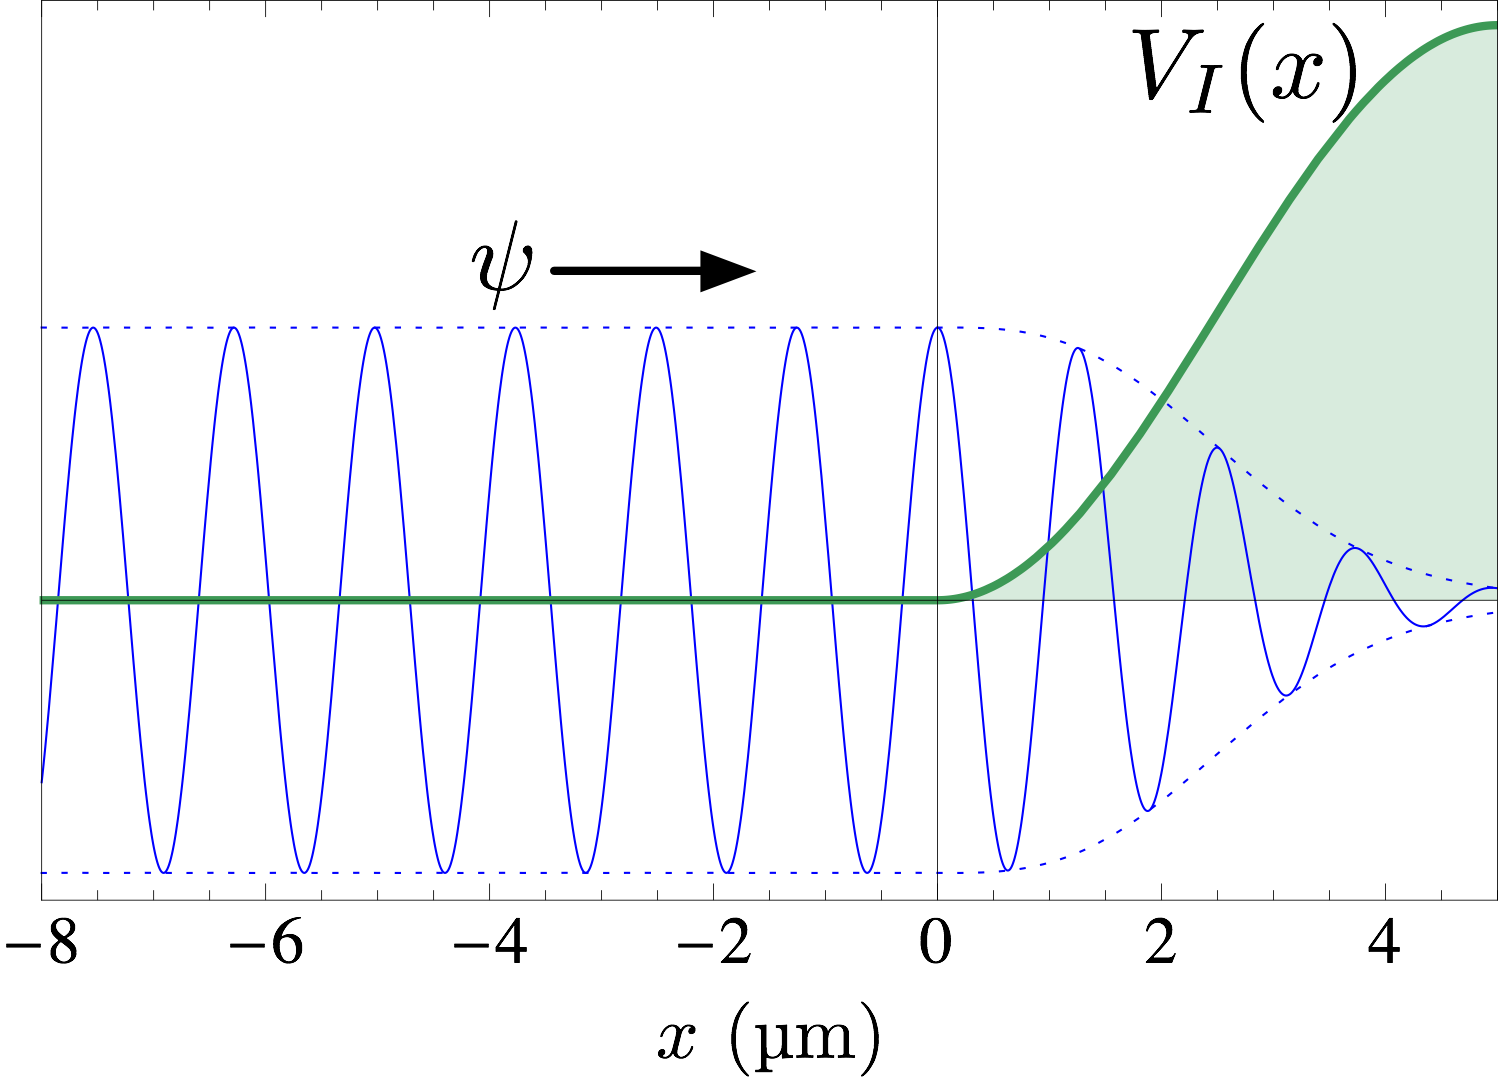
\includegraphics[width=8cm]{AbsorbingBoundarySchematic}
    \caption{
        \label{BackgroundTheory:AbsorbingBoundarySchematic}
        Schematic diagram illustrating the use of an absorbing boundary layer. A right-travelling wave is incident on the absorbing boundary layer which is given by the potential $V(x) = -i V_I(x)$. The wave is attenuated as it crosses the absorbing boundary layer.
    }
\end{figure}

An absorbing boundary layer of finite thickness can only be effective over a finite range of incident wavenumbers. Incident wavefunctions with large wavelengths (low wavenumbers) will be reflected from the absorbing boundary layer due to the rapid variation in the potential over a wavelength. Incident wavenumbers with very short wavelengths (high wavenumbers) will be transmitted through the absorbing boundary layer due to the finite amount of time spent in the absorbing boundary layer by any point on the phase-front.  Using this argument \citet{Neuhasuer:1989} showed that the approximate range of wavenumbers over which an absorbing boundary layer will be effective is
\begin{align}
    \label{BackgroundTheory:AbsorbingBoundaryKEffectiveRange}
    \left( \frac{M \overline{V_I}}{\hbar^2 \Delta x}\right)^{\frac{1}{3}} \ll k \ll \frac{4 M \overline{V_I} \Delta x}{\hbar^2},
\end{align}
where $\overline{V_I}$ is a representative value of $V_I(x)$. The maximum and minimum limits for the wavenumber are respectively due to the requirements of negligible transmission and reflection. Although cast in terms of the wavenumber, \eqref{BackgroundTheory:AbsorbingBoundaryKEffectiveRange} is equivalent to (26) in~\citep{Neuhasuer:1989}. While not its purpose, \sectionref{MethodsAppendix:MomentumDensityFluxExampleCalculation} demonstrates how to calculate the reflection and transmission coefficients as a function of wavenumber for arbitrary absorbing boundary layers.

The use of absorbing boundary layers must be slightly modified for use in phase-space methods such as those discussed in \sectionref{BackgroundTheory:StochasticPhaseSpaceMethods}. In these cases simply adding an absorbing boundary layer to the potential would lead to unphysical results as the absorbing potential would not discriminate between real particles in a mode and the virtual particles which represent the fundamental vacuum fluctuations inherent in the field. An appropriate way of handling this problem is to add a position-dependent loss term to the master equation of the form
\begin{align}
    \label{BackgroundTheory:PhaseSpaceAbsorbingBoundaryLayer}
    \frac{d \hat{\rho}}{dt} &= \int d \vect{x}\, \frac{2}{\hbar}V_I(\vect{x})\mathcal{D}[\hat{\Psi}(\vect{x})]\hat{\rho},
\end{align}
where $\mathcal{D}$ is the usual decoherence superoperator. This master equation term leads to the same imaginary potential term in the equations of motion for the field operator with an additional noise term the for Truncated Wigner and Q function methods that restores the vacuum fluctuations that would otherwise be lost.

\parasep

In most of this thesis it is only the immediate vicinity of the BEC that is under consideration and absorbing boundary layers are used to restrict the computational domain to this region.  As the use of absorbing boundary layers is a technical issue not related to the underlying physics, they are not included in equations of motion given in this thesis but should be understood to be included when simulations are performed.  

% While direct application of absorbing boundary layers permit the study of dynamics near the BEC, in \chapterref{TransverseProfile} the transverse profile of the atom laser a large distance from the BEC is considered.  In this case a different strategy must be used to avoid the $N_\text{pts} \propto t^3$ scaling discussed above.  Such a strategy is discussed in \sectionref{TransverseProfile:DropGP}.



\chapter{On the production of entangled beams from a metastable helium BEC}
\label{Peaks}
\graphicspath{{Figures/Peaks/}{Figures/Common/}}

In this chapter we investigate the production of paired atom laser beams from a metastable helium condensate due to an unusual scattering process.  Radio-frequency outcoupling is used to extract atoms from a Bose-Einstein condensate to initiate scattering between trapped and untrapped atoms.  The unequal strengths of the interactions for different internal states allows an energy-momentum resonance which leads to the scattering of atoms from the zero-velocity condensate into modes of opposite momenta.  This process is shown to be the result of dynamical instabilities within the condensate that originate from a process analogous to optical parametric down-conversion, giving rise to entanglement between the unstable modes.  These unstable modes are outcoupled to form scattered beams well-separated from the main atom laser profile, which are observed experimentally.

The results presented in \sectionref{Peaks:PerturbativeApproach} of this chapter are in preparation for submission, while the results presented in \sectionref{Peaks:3DCalculation} of this chapter have been published in \citet{Dall:2009}.  All of the theoretical work in these papers was my own work with the exception of the classical propagation discussed at the end of \sectionref{Peaks:AbsorbingBoundaryTricks}.

%FIXME: Somewhere in this chapter we should reference the work of \citet{Pu:2000,Duan:2000}.

\section{Introduction}
Sources of matter waves gained a dramatic improvement with the achievement of Bose-Einstein condensation (BEC) in dilute gases and the development of the atom laser \citep{Anderson:1995vn,Mewes:1997}. Like optical lasers before them, atom lasers can produce Heisenberg-limited beam profiles \citep{Busch:2002zr,Riou:2006uq} and promise high spectral density through their dramatically lower linewidth \citep{Wiseman:1997ba}. Another exciting possibility resulting from having such a coherent source of atoms is the generation of nonclassical matter waves such as entangled beams. Entangled beams are useful for tests of quantum mechanics and are required to perform Heisenberg-limited interferometry \citep{Dowling:1998,Reid:1988}.  In this chapter, we show that the asymmetric scattering lengths between internal states of metastable helium (He*) cause well-defined peaks in the output of an atom laser.  These peaks are due to a dynamical instability in the condensate that originates from a process that generates entanglement.

A nonlinear process is required to produce entanglement, and one of the advantages of atomic systems over optical systems is that there are strong inherent nonlinearities due to atomic interactions, although these interactions can also lead to complications. These nonlinearities allow certain analogues of nonlinear optical experiments such as four-wave mixing, parametric down-conversion and Kerr squeezing to be performed directly in the atomic sample \citep{WallsMilburn}. All of these produce non-classical states in optical systems. Four-wave mixing in a trapped BEC has been demonstrated experimentally in configurations where three distinct momentum states generated a fourth \citep{Deng:1999qy} and where two momentum states generated a pair of correlated atomic beams \citep{Vogels:2002}. These experiments demonstrated that the output phase was coherent, but the correlation properties were not measured. More recently the pair correlations in a spontaneous scattering of two colliding condensates were measured using the single-atom detectors available for He* atoms \citep{Perrin:2007}.

Using these existing sources of entangled pairs of atoms for interferometric experiments will be complicated by the high densities of the sources, where the nonlinearities that generated the correlations ultimately degrade the long-term coherence of the sample. While recent experiments have increased the coherence of atom interferometers by several orders of magnitude by reducing the nonlinearities with a Feschbach resonance \citep{Fattori:2008,Gustavsson:2008}, this precludes the production of entangled pairs.  In the scheme presented here the nonlinear interactions are used to drive dynamical instabilities in the condensate, but the resulting untrapped beams that propagate in free space are dilute, potentially avoiding the decoherence problem.  We show that pairs of beams can be produced simply by the process of radio-frequency (rf) outcoupling from a He* BEC, without the need for Feschbach resonances or scattering pulses.  Unlike previous methods, which required pairs of atoms travelling at high kinetic energies as a source, this process involves scattering between atoms initially in the same zero-momentum state to create states with nonzero momentum.  Semiclassical and field-theoretic simulations of the experiment show that the beams are generated by the same parametric down-conversion process that generates entangled optical beams.  Although the beams in the present experiment will not retain all of the original non-classical correlations produced by the dynamical instabilities, some will remain and a future experiment is proposed that may enable the full correlations produced by the dynamical instabilities to be extracted from the condensate.

\section{The metastable helium `Peaks' experiment}
\label{Peaks:ExperimentalSetup}

The experimental setup for creating He* BEC has been reported elsewhere \citep{Dall:2007a}, and discussed earlier in this thesis (see \sectionref{TransverseProfile:He*Experiment}). The experiment discussed in this section was performed by \emph{Robert Dall}, \emph{Lesa Byron} and \emph{Andrew Truscott} at the Research School of Physics and Engineering, ANU.

Starting from an almost pure BEC containing up to $2\times 10^6$ atoms, an atom laser beam was created by using rf photons to spin flip the BEC atoms from the $m_F=1$ magnetically trapped state to the $m_F=0$ untrapped state.  After outcoupling, atoms in the atom laser beam fell under gravity for a distance of $\unit[4]{cm}$ until they hit a double-stacked multichannel plate (MCP). The phosphor screen was imaged with a charge-coupled-device (CCD) camera with a resolution of approximately $\unit[150]{\micro m}$ at the MCP. To remove any nonuniformities caused by spatial variations in the gain of the MCP, all images were divided by a flat-field image produced by dropping atoms from a MOT onto the detector. Since the MOT temperature is of order $\sim\unit[1]{mK}$, the spatial profile of the MOT uniformly illuminates the MCP. Although $m_F=-1$ atoms are produced by the outcoupling, especially for high rf powers, they are in general accelerated away from the detector by the magnetic trap field. Those that are accelerated towards the detector do not show up in the images since they arrive much earlier than the CCD trigger time.

\figureref{Peaks:ExperimentalResults} shows the dramatic change in the atom laser spatial profile when the dynamical instabilities in the condensate are excited.  In the case of low outcoupling Rabi frequencies (upper row), this process does not occur and we see the usual double-peaked He*-atom laser profile \citep{Dall:2007} (see also \sectionref{TransverseProfile:Helium}). When the Rabi frequencies are high enough to drive the instabilities (lower row), the atoms in the atom laser beam are scattered to form a halo around the main atom laser beam.  Due to conservation of energy, the outer diameter of this halo corresponds to a maximum kinetic energy given by the chemical potential.  As well as the ring structure, four peaks are observed on the outskirts of the profile.
% Each peak contains 11\%--14\% of the total outcoupled atoms, in agreement with the value of 11\% obtained from the simulation results shown in the lower row of \figureref{Peaks:ExperimentalResults}.

These peaks arise from two momentum-correlated cones of particles scattering out of the condensate and falling to the detector, as shown in \figureref{Peaks:Schematic}.  The cones themselves are generated by a dynamical instability that populates momentum modes lying along the weak trapping axis, which expand to rings due to the mean-field repulsion in the tight trapping direction as they leave the BEC.  Atoms in these cones then fall under gravity onto the detector, where the time-integrated flux is converted to a spatial density distribution, and each momentum ring appears as a double peak.  The background halo is produced during the initial switch-on of the atom laser during which the peaks produced by the instabilities sweep in position from the main atom laser profile towards their final position in \figureref{Peaks:ExperimentalResults}.

A summary of the relevant parameters of the experiment is given in \tableref{Peaks:ExperimentalParameters}.

\begin{figure}
    \centering
        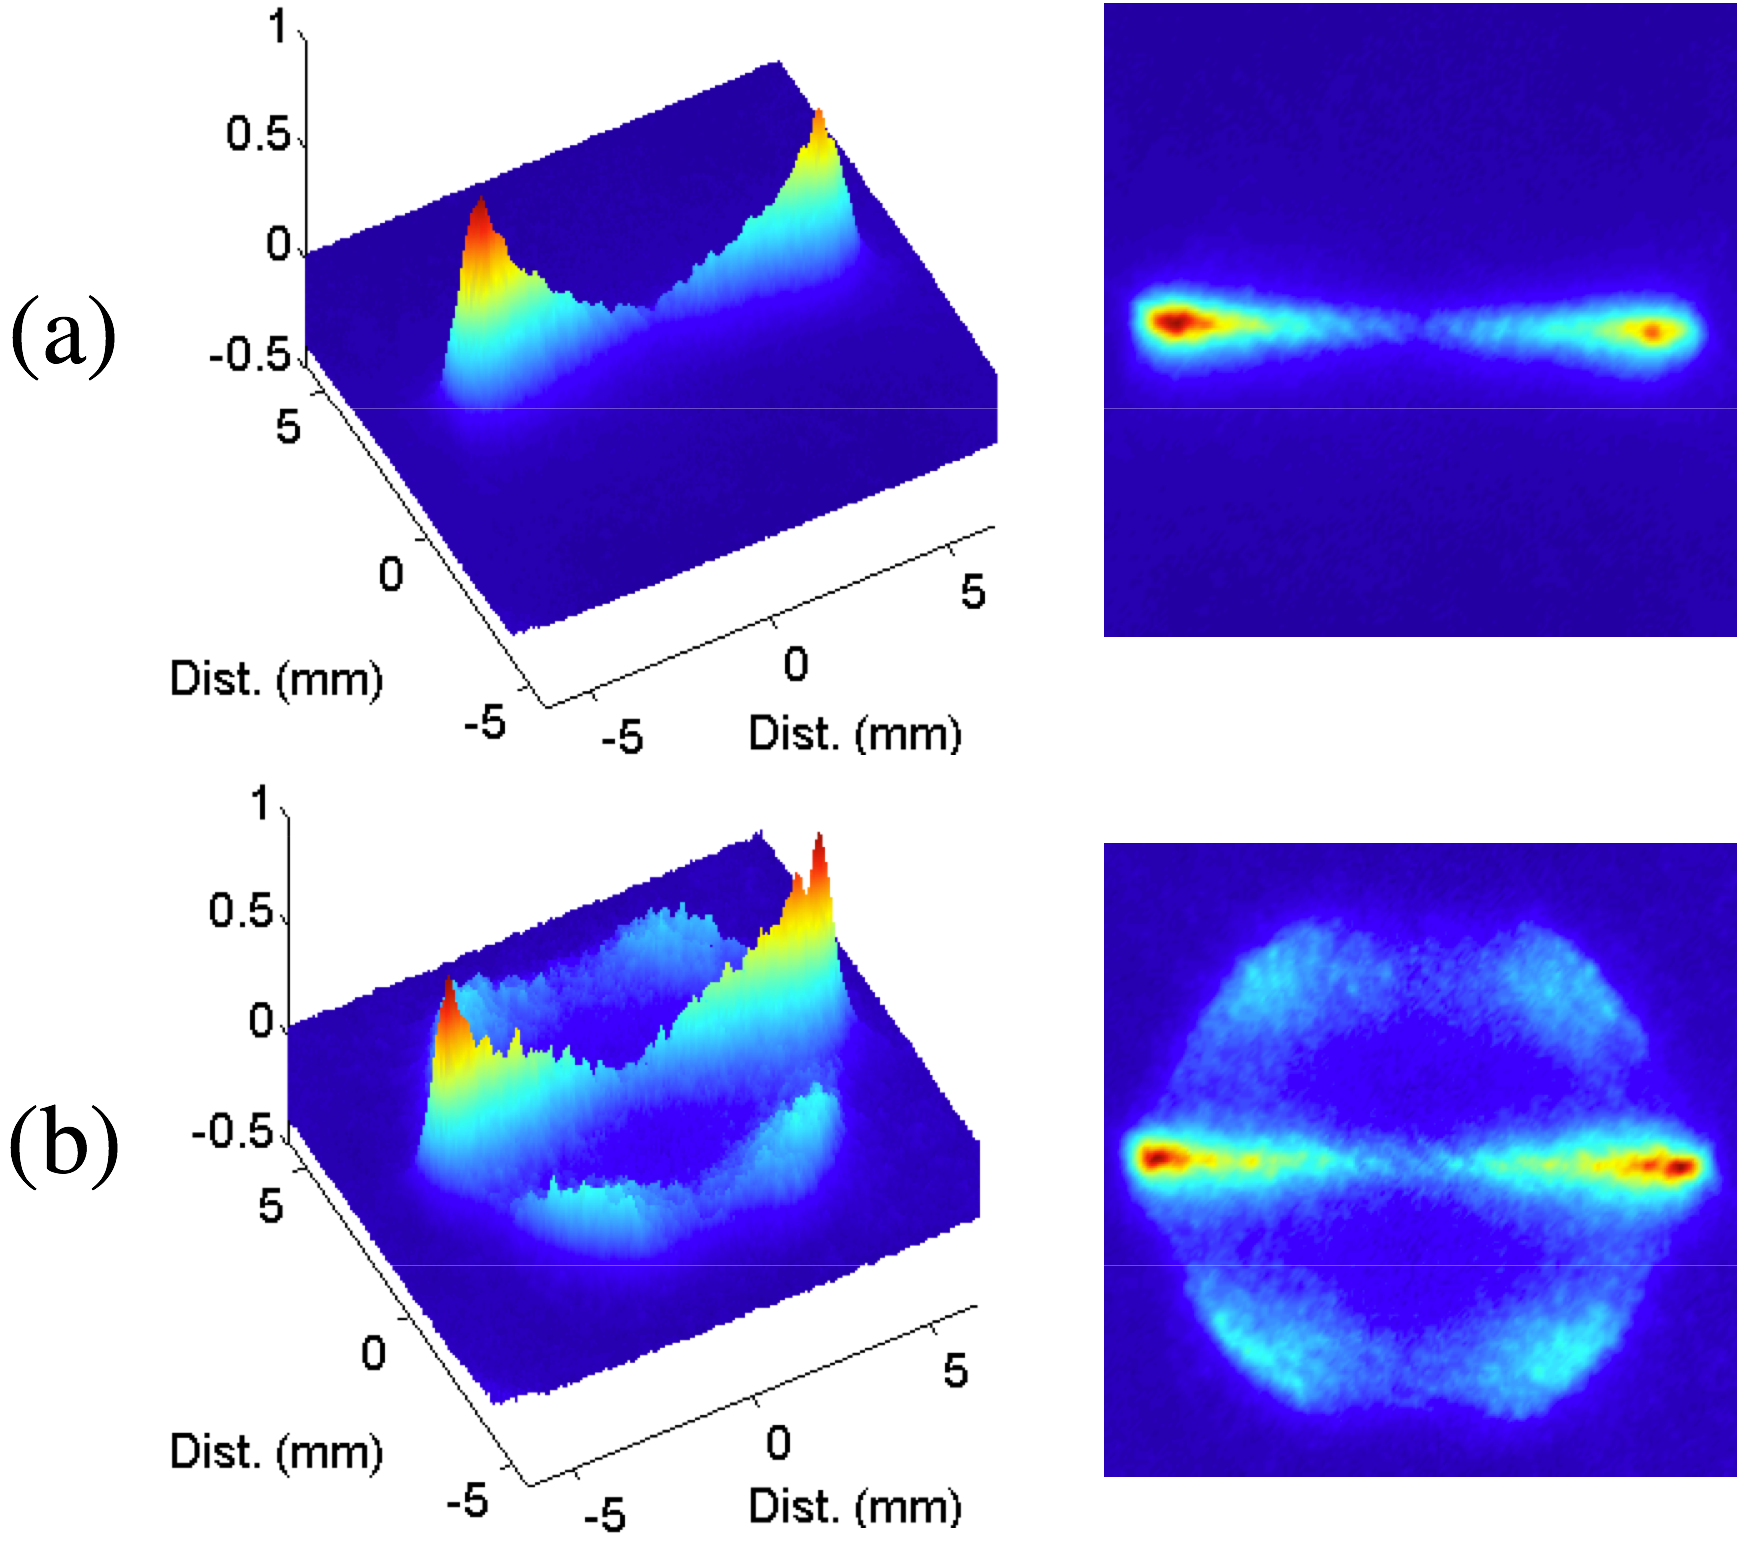
\includegraphics[height=3in]{ExperimentalResults}
    \caption{Experimental results. The difference between (a) and (b) is that the outcoupling Rabi frequency has been increased by an order of magnitude in (b).}
    \label{Peaks:ExperimentalResults}
\end{figure}

\begin{figure}
    \centering
        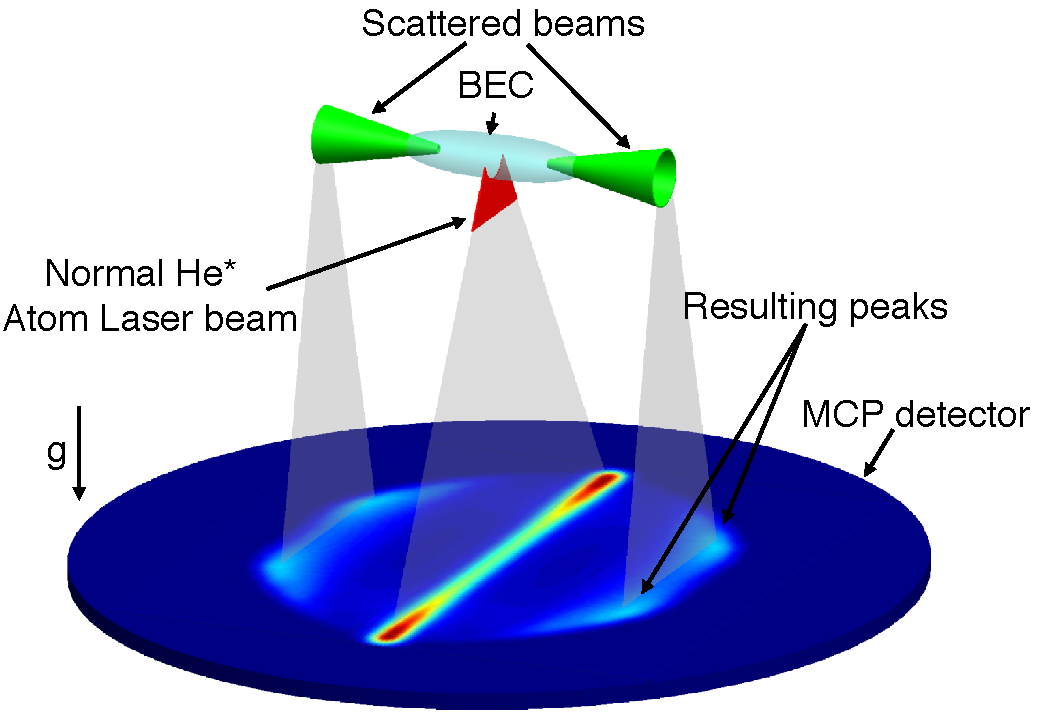
\includegraphics[height=3in]{Schematic}
    \caption{Schematic of the experimental setup}
    \label{Peaks:Schematic}
\end{figure}


\begin{table}
    \centering
    \begin{tabular}{cc}
    \toprule
    Parameter & Value\\
    \midrule
    Condensate number & $N = 2\times 10^6$\\
    Radial trapping frequency & $\omega_r = 2 \pi \times \unit[1020]{Hz}$\\
    Axial trapping frequency & $\omega_z = 2\pi \times \unit[55]{Hz}$\\
    Outcoupling Rabi frequency & $\Omega = 2\pi \times \unit[6.5]{kHz}$\\
    \bottomrule
    \end{tabular}
    \caption{Experimental parameters for the metastable helium BEC under consideration.}
    \label{Peaks:ExperimentalParameters}
\end{table}

\section{Overview of Bogoliubov theory}
\label{Peaks:ElementaryExcitations}

The observed features in the atom laser profile presented in the previous section are caused by a dynamical instability in the condensate. The modes that are dynamically unstable are identified in the next section, in which the excitation spectrum of the condensate is obtained. In this section an overview is given of the Bogoliubov theory which is used to obtain the excitation spectrum of the condensate and to determine its stability. More comprehensive treatments of the Bogoliubov theory are given in \citep{PethickSmith} and in a number of review articles \citep{Leggett:2001,Ozeri:2005,Proukakis:2008}.

The problem is to determine the response of the condensate to small fluctuations about the mean-field. Typically the condensate is stable to such fluctuations, and their energy spectrum determines the phase and group velocities of the excitations.  In the case that the condensate is dynamically unstable some modes will undergo exponential growth, which corresponds to the generalised energy spectrum containing nonzero imaginary components. As a concrete example of the techniques demonstrated in this section, we consider a single-component condensate described by the Hamiltonian
\begin{align}
    \label{Peaks:ElementaryExcitationsExampleHamiltonian}
    \hat{H} &= \int d \bm{x}\, \hat{\Psi}^\dagger \left( -\frac{\hbar^2 \nabla^2}{2 M} + V(\bm{x}) + \frac{1}{2} U \hat{\Psi}^\dagger \hat{\Psi} - \mu \right) \hat{\Psi},
\end{align}
where an arbitrary energy offset $\mu$ has been included. This term is introduced for calculational reasons and has no physical influence on the Hamiltonian\footnote{The energy offset cannot affect any observable expectation values as although it contributes a different energy offset for states with different total number, these states are uncoupled due to the conservation of particle-number.}.

The principal idea in finding the excitation spectrum of \eqref{Peaks:ElementaryExcitationsExampleHamiltonian} is to take advantage of the usefulness of the Gross-Pitaevskii equation in describing the mean-field of the condensate to enable the quantum-mechanical fluctuations about the mean-field to be considered. To this end the deviation operator $\delta \hat{\Psi} = \hat{\Psi} - \Psi$ is defined, where $\Psi = \mean{\hat{\Psi}}$, and $\delta \hat{\Psi}$ is considered to be a small quantity\footnote{For $\delta\hat{\Psi}$ to be considered a small quantity, the mean field $\mean{\hat{\Psi}}$ must be non-zero. However the state of condensates with a large number of atoms is well approximated by either a state with well-defined total number or as a mixture over global phase of coherent states (see \sectionref{BackgroundTheory:SymmetryBreaking}), for both of these the mean field $\mean{\hat{\Psi}}$ is zero. Despite this, as any \emph{physical} expectation value is independent of the choice of global phase, the analysis presented here can be performed for any coherent state and the results then averaged over the global phase. As all physical expectation values are independent of the global phase this averaging step cannot change the results and can be omitted.}. The Hamiltonian \eqref{Peaks:ElementaryExcitationsExampleHamiltonian} can then be expanded in powers of $\delta \hat{\Psi}$,
\begin{align}
    \label{Peaks:HamiltonianPowerSeriesExpansion}
    \hat{H} &= \hat{H}_0 + \hat{H}_1 + \hat{H}_2 + \hat{H}_3 + \hat{H}_4,
\end{align}
where $\hat{H}_n$ contains terms of order $(\delta\hat{\Psi})^n$. The excitation spectrum of the Hamiltonian $\hat{H}$ is then approximately given by the eigenvalue spectrum of the lowest order nonzero term in \eqref{Peaks:HamiltonianPowerSeriesExpansion}.

The zeroth order term in \eqref{Peaks:HamiltonianPowerSeriesExpansion}
\begin{align}
    \hat{H}_0 &= \int d \bm{x}\, \Psi^* \left( -\frac{\hbar^2 \nabla^2}{2M} + V(\bm{x}) + \frac{1}{2} U \big|\Psi\big|^2 - \mu \right) \Psi
\end{align}
is simply a constant and represents the total energy of the unexcited mean-field. The first order term is of the form
\begin{align}
    \hat{H}_1 &= \int d \bm{x}\, \delta \hat{\Psi}^\dagger \left(i \hbar \frac{\partial \Psi}{\partial t} \right)  + \int d \bm{x}\, \left(i \hbar \frac{\partial \Psi}{\partial t} \right)^* \delta \hat{\Psi},
\end{align}
where the mean-field $\Psi$ evolves as
\begin{align}
    i \hbar \frac{\partial\Psi}{\partial t} &= \left(-\frac{\hbar^2 \nabla^2}{2 M} + V(\bm{x}) + U \big| \Psi\big|^2 - \mu \right) \Psi.
\end{align}

Although the first order term $\hat{H}_1$ is nonzero, it does not affect the evolution of the deviation operator:
\begin{align}
    i \hbar \frac{\partial }{\partial t}\hat{\Psi} &= \comm{\hat{\Psi}, \hat{H}}\\
    i \hbar \frac{\partial }{\partial t}\delta{\hat{\Psi}} + i \hbar \frac{\partial \Psi}{\partial t} &= \comm{\Psi, \hat{H}} + \comm{\delta\hat{\Psi}, \hat{H}}\\
    i \hbar \frac{\partial }{\partial t}\delta \hat{\Psi} &= \comm{\delta \hat{\Psi}, \hat{H}} - i \hbar \frac{\partial  \Psi}{\partial t}\\
    &= \comm{\delta \hat{\Psi}, \hat{H}_1} + \comm{\delta \hat{\Psi}, \hat{H}_2 + \hat{H}_3 + \hat{H}_4} - i \hbar \frac{\partial\Psi }{\partial t}\\
    &= i \hbar \frac{\partial \Psi}{\partial t} + \comm{\delta \hat{\Psi}, \hat{H}_2 + \hat{H}_3 + \hat{H}_4} - i \hbar \frac{\partial \Psi}{\partial t}\\
    &= \comm{\delta \hat{\Psi}, \hat{H}_2 + \hat{H}_3 + \hat{H}_4}. \label{Peaks:DeviationOperatorEvolution}
\end{align}
As $\hat{H}_1$ does not occur in \eqref{Peaks:DeviationOperatorEvolution}, it does not affect the evolution of the deviation operators and so will not contribute to the excitation spectrum\footnote{Typical treatments of the Bogoliubov theory consider the restricted case of a static condensate density and choose $\mu$ as the chemical potential such that $\displaystyle \frac{\partial \Psi}{\partial t} = 0$, and hence $\hat{H}_1=0$. As shown by \eqref{Peaks:DeviationOperatorEvolution}, this choice of $\mu$ is unnecessary as $\hat{H}_1$ does not influence the evolution of $\delta\hat{\Psi}$, \emph{independent} of the choice of $\mu$ and even in the general case of a non-stationary mean field. This latter case is considered in \sectionref{Peaks:PerturbativeApproach}.}.

The first physically important term in \eqref{Peaks:HamiltonianPowerSeriesExpansion} is
\begin{align}
    \begin{split}
        \hat{H}_2 &= \int d \bm{x}\, \delta \hat{\Psi}^\dagger \left(-\frac{\hbar^2 \nabla^2}{2 M} + V(\bm{x}) + 2 U\big|\Psi\big|^2 -\mu \right)\delta\hat{\Psi}\\
         &\relphantom{=} + \frac{1}{2} U\int d \bm{x}\, \left(\Psi^2 \delta \hat{\Psi}^\dagger\delta \hat{\Psi}^\dagger  +  (\Psi^*)^2 \delta \hat{\Psi} \,\delta \hat{\Psi}\right).
    \end{split}
    \label{Peaks:HamiltonianPowerSeriesQuadraticTerm}
\end{align}
As the deviation operator $\delta \hat{\Psi}$ is small in some sense compared to the mean field $\Psi$, the higher-order contributions $\hat{H}_3$ and $\hat{H}_4$ to the total Hamiltonian can then be neglected compared to $\hat{H}_2$. The excitation spectrum of the condensate about the mean field $\Psi$ is then given by the energy spectrum of $\hat{H}_2$.

To avoid directly solving the infinite dimensional eigenvalue problem $\hat{H}_2 \ket{\Psi} = E \ket{\Psi}$ for the condensate excitation spectrum, it is desired to apply a linear transformation to $\hat{H}_2$ that will diagonalise it in the form
\begin{align}
    \label{Peaks:QuadraticHamiltonianAnsatz}
    \hat{H}_2 &= \sum_i \hbar \omega_i \hat{\Lambda}_i^\dagger \hat{\Lambda}_i^{\phantom{\dagger}},
\end{align}
for some boson annihilation operators $\hat{\Lambda}_i$ and real frequencies $\omega_i$. In this form, the Hamiltonian can be simply interpreted as representing a set of modes with energies $\hbar \omega_i$, which is the condensate excitation spectrum. The eigenvalues of $\hat{H}_2$ can also be identified as $\{n \hbar \omega_i : n > 0 \}$. It is not possible in general to transform $\hat{H}_2$ into the form \eqref{Peaks:QuadraticHamiltonianAnsatz} if the Hamiltonian possesses any instabilities \citep{Leonhardt:2003}, however one frequently considers the excitation spectrum of the ground state which is stable by definition and in this case such a transformation is always possible.

In the general case, we look for the operators $\hat{\Lambda}_i$ satisfying
\begin{align}
    \label{Peaks:ElementaryExcitationsEvolution}
    i \hbar \frac{\partial }{\partial t}\hat{\Lambda}_i &= \comm{\hat{\Lambda}_i, \hat{H}_2 } = - \hbar \omega_i \hat{\Lambda}_i
\end{align}
where $\omega_i$ is real if and only if $\hat{\Lambda}_i$ is a boson annihilation operator \citep{Leonhardt:2003}. In the case that $\omega_i$ is complex, boson annihilation operators can be constructed from the $\hat{\Lambda}_i$ as discussed in \appendixref{FloquetAppendix}. Hence $\hbar\omega_i$ can be considered to be a generalised energy spectrum of the condensate where nonzero imaginary components correspond to dynamical instabilities of the condensate. Note that although the eigenvalues of $\hat{H}_2$ must be real as it is Hermitian, the eigenvalues of \eqref{Peaks:ElementaryExcitationsEvolution} need not be real. For example, the Hamiltonian for degenerate parametric down-conversion $\hat{H} = \hbar\chi \left(\hat{a}\hat{a} + \hat{a}^\dagger \hat{a}^\dagger \right)$ is Hermitian but its eigenvalues in \eqref{Peaks:ElementaryExcitationsEvolution} are pure imaginary. In this case the occupation of the mode $\hat{a}$ undergoes exponential growth. The case of complex eigenvalues $\omega_i$ is discussed further in \sectionref{Peaks:ExperimentEigenvalues} and \appendixref{FloquetAppendix}.

Equation \eqref{Peaks:ElementaryExcitationsEvolution} is most easily solved by expanding the $\hat{\Lambda}_i$ in a complete, linearly independent basis $\{\hat{\Upsilon}_j\}$ such that $\hat{\Lambda}_i = \bm{c}_i^\dagger \hat{\bm{\Upsilon}}$ where $\bm{c}_i$ is a complex vector, $\bm{c}_i^\dagger$ denotes the conjugate-transpose, and $\hat{\bm{\Upsilon}}$ is the column vector formed by the complete basis $\{\hat{\Upsilon}_j\}$. For the case of \eqref{Peaks:HamiltonianPowerSeriesQuadraticTerm}, an appropriate basis is $\{\hat{\Upsilon}_j\} = \{\delta\hat{\Psi}, \delta\hat{\Psi}^\dagger\}$. As the Hamiltonian $\hat{H}_2$ is quadratic, its commutator with every operator $\hat{\Upsilon}_j$ will be linear in the operators $\{\hat{\Upsilon}_j\}$. Defining the complex matrix $\mathcal{H}$ to represent this relationship as
\begin{align}
    \label{Peaks:ScriptHRelationshipToHamiltonian}
    \sum_k \mathcal{H}_{jk} \hat{\Upsilon}_k &= \comm{\hat{\Upsilon}_j, \hat{H}_2}
\end{align}
permits \eqref{Peaks:ElementaryExcitationsEvolution} to be recast as an eigenvalue problem in $\mathcal{H}$,
\begin{align}
    \comm{\bm{c}_i^\dagger \hat{\bm{\Upsilon}}, \hat{H}_2} &= \bm{c}_i^\dagger \mathcal{H} \hat{\bm{\Upsilon}} = - \hbar \omega_i \bm{c}_i^\dagger \hat{\bm{\Upsilon}}, \label{Peaks:ElementaryExcitationsEigenvalueProblemWithOperators}\\
    \implies \bm{c}_i^\dagger \mathcal{H} &= - \hbar \omega_i \bm{c}_i^\dagger \label{Peaks:ElementaryExcitationsEigenvalueProblem}
\end{align}
where the last line follows as the components of $\hat{\bm{\Upsilon}}$ are linearly independent. If the mean-field $\Psi$ is time-independent, then the matrix $\mathcal{H}$ will also be time-independent and \eqref{Peaks:ElementaryExcitationsEigenvalueProblem} represents an eigenvalue problem for the left eigenvectors $\bm{c}_i^\dagger$ and eigenvalues $-\hbar \omega_i$ of the matrix $\mathcal{H}$. If the mean-field $\Psi$ simply evolves due to a global phase rotation, this can be cancelled by appropriate choice of the arbitrary energy offset $\mu$ making $\mathcal{H}$ time-independent.  In the case of the condensate ground state, that offset will be the chemical potential of the condensate. The eigenvalues $\{\hbar \omega_i\}$ then represent the generalised excitation spectrum of the condensate about the mean field, which was to be determined. 

It is important to note that for the eigenvalues of $\mathcal{H}$ to determine the solution to \eqref{Peaks:ElementaryExcitationsEvolution} the matrix $\mathcal{H}$ must be constant. In the next section these techniques will be generalised to the case of a \emph{periodic} mean-field in which the time-dependence of the matrix $\mathcal{H}$ cannot be removed by any analytic transformation.

In the case of a homogenous condensate ($V(\bm{x}) = 0$) the matrix $\mathcal{H}$ can be diagonalised analytically to give the condensate excitation spectrum as
\begin{align}
    \hbar \omega(\bm{k}) &= \sqrt{\varepsilon(\bm{k})\left(\varepsilon(\bm{k}) + 2 n U \right)},
    \label{Peaks:BogoliubovSpectrum}
\end{align}
where $\bm{k}$ is the wavevector, $\displaystyle \varepsilon(\bm{k}) = \frac{\hbar^2 \bm{k}^2}{2 M}$ is the free-particle energy spectrum and $n = \big|\Psi \big|^2$ is the condensate density. Equation~\eqref{Peaks:BogoliubovSpectrum} is known as the Bogoliubov excitation spectrum \citep{Bogoliubov:1947}.  

In the limit of large wavenumbers, the Bogoliubov excitation spectrum becomes
\begin{align}
    \hbar \omega(\bm{k}) &\approx \varepsilon(\bm{k}) + n U,
\end{align}
i.e. that of a free particle shifted by the mean field experienced by the rest of the condensate.  It is important to note that this spectrum is that of \emph{excitations} to the condensate, not of particles \emph{added} to the system with wavenumber $\bm{k}$.  The energy of a thermal particle added to the system will be given by the excitation spectrum \emph{plus} the chemical potential, i.e. the energy required to add an atom to the system $n U$.  In the limit of large wavenumbers the energy of a thermal particle is
\begin{align}
    E_\text{thermal}(\bm{k}) &\approx \varepsilon(\bm{k}) + 2 n U.
    \label{Peaks:ThermalParticleEnergySpectrum}
\end{align}
Thermal particles therefore experience twice the mean-field experienced by the condensate.  This is because the thermal atoms can be distinguished from the atoms in the condensate, while the atoms in the condensate cannot be distinguished from one another.

The interested reader is referred to the review paper by \citet{Ozeri:2005} for further details about Bogoliubov theory in Bose-Einstein condensates.

\section{Condensate excitations in the perturbative regime}
\label{Peaks:PerturbativeApproach}
%While the argument in the previous section gives a qualitative explanation for the four-wave mixing process observed in He*, it is not entirely satisfying. In this section an approximate analytic expression for the excited modes of the He* system will be obtained and investigated using Bogoliubov stuff.

The observed features in the atom laser profile presented in \sectionref{Peaks:ExperimentalSetup} are caused by a dynamical instability in the condensate that causes the formation of momentum excitations in a narrow range of momenta along the weak trapping axis. During outcoupling these excitations are accelerated along the tight trapping directions forming the momentum cones pictured in \figureref{Peaks:Schematic}. The detection process vertically integrates this momentum profile leading to the observed peaks in \figureref{Peaks:ExperimentalResults}.

The dynamical instability is due to the significantly different scattering lengths between the Zeeman levels of He*. In a later section a full multimode quantum-field calculation will be discussed and its results presented, but it is enlightening to first consider a simplified model in which the energy spectrum (and stability) of small excitations to the condensate can be obtained.

The simplified model to be considered is that of a homogenous spinor condensate consisting of two levels with Rabi oscillations coupling the two levels. The approximation that the condensate is homogenous (known as the local density approximation \cite{Stamper-Kurn:1999,Zambelli:2000}) is justified if the excitations under consideration have wavelengths much smaller than the Thomas-Fermi radius in that dimension. The local density approximation will hold for this system along the axial direction as the axial momentum of the features observed in \figureref{Peaks:ExperimentalResults} corresponds to an excitation wavelength of $\sim \unit[5]{\micro m}$, significantly smaller than the Thomas-Fermi radius in the axial direction of $z_\text{TF} = \unit[175]{\micro m}$. 

The second approximation made in this model is to neglect the antitrapped state $m_F=-1$. Any density in this state leaves the condensate very rapidly due to the combined effects of both the mean-field repulsion and the magnetic field gradient. A classical particle in the centre of the condensate under the influence of the same effective potential experienced by the $m_F=-1$ atoms would reach a momentum equal to the momentum width of the condensate (and hence no longer be able to couple to the stationary atoms in the middle of the condensate) in $\sim\unit[80]{\micro s}$, significantly shorter than the inverse Rabi frequency of $\sim \unit[300]{\micro s}$.

With these approximations made, the Hamiltonian for this system is
\begin{align}
    \label{Peaks:InitialHamiltonian}
    \begin{split}
    \hat{H} &= \sum_i \int d\bm{x}\, \hat{\Psi}_i^\dagger \left(\frac{-\hbar^2 \nabla^2}{2 M} - \mu\right)\hat{\Psi}_i^{\phantom{\dagger}} + \frac{1}{2} \sum_{i j} U_{i j}\int d\bm{x}\, \hat{\Psi}_i^\dagger \hat{\Psi}_j^\dagger \hat{\Psi}_j^{\phantom{\dagger}} \hat{\Psi}_i^{\phantom{\dagger}}\\
            &\phantom{=} + \hbar \Omega \int d\bm{x}\, \left(\hat{\Psi}_1^\dagger \hat{\Psi}_0^{\phantom{\dagger}} + \hat{\Psi}_0^\dagger \hat{\Psi}_1^{\phantom{\dagger}}\right),
    \end{split}
\end{align}
where $U_{ij} = 4\pi \hbar^2 a_{ij}/M$ is the nonlinear interaction strength, $a_{ij}$ is the \emph{s}-wave scattering length between internal states $i$ and $j$, $\Omega$ is the Rabi frequency which is taken to be real, and $\mu$ is an energy offset which has been included to cancel the global phase rotation which would otherwise be present. The equations of motion corresponding to this Hamiltonian are
\begin{subequations}
    \label{Peaks:OperatorEquationsOfMotion}
    \begin{align}
    i \hbar \frac{\partial }{\partial t}\hat{\Psi}_1  &= -\frac{\hbar^2}{2M}\nabla^2 \hat{\Psi}_1  + U \left(\hat{\Psi}_1^\dagger \hat{\Psi}_1^{\phantom{\dagger}} + \hat{\Psi}_0^\dagger \hat{\Psi}_0^{\phantom{\dagger}}\right) \hat{\Psi}_1 + \hbar \Omega \hat{\Psi}_0 - \mu \hat{\Psi}_1,  \\
    i \hbar \frac{\partial }{\partial t}\hat{\Psi}_0 &= -\frac{\hbar^2}{2M} \nabla^2 \hat{\Psi}_0 + U \left(\hat{\Psi}_1^\dagger \hat{\Psi}_1^{\phantom{\dagger}} + \kappa \hat{\Psi}_0^\dagger \hat{\Psi}_0^{\phantom{\dagger}} \right) \hat{\Psi}_0 + \hbar \Omega \hat{\Psi}_1 - \mu \hat{\Psi}_0,
    \end{align}
\end{subequations}
where $U=U_{11}=U_{10}$ and $\kappa = U_{00}/U_{11}$.  For metastable helium in the $F=1$ manifold, $\kappa \approx 0.74$ \citep{Leo:2001}, while for Rubidium in the $F=1$ manifold, $\kappa = 1.002$ \cite{Kempen:2002,Widera:2006}.

\subsection{The dynamical steady-state}
\label{Peaks:MeanFieldPeriodicity}

The excitation spectrum of a condensate can be obtained by approximating each field operator to be a c-number (the mean-field) plus a small fluctuation term, and then either diagonalising the Hamiltonian \cite{Bogoliubov:1947,FetterWalecka} or diagonalising the linearised equations of motion for the fluctuations themselves (see \sectionref{Peaks:ElementaryExcitations}). It is the latter approach that will be taken here, but with the difference that the mean-field about which the linearisation procedure will take place is itself \emph{time-dependent}.

The mean-field state that we wish to consider is one that corresponds to the state of the BEC in the experiment. At $t=0$ all of the population in this state will be in the $m_F=1$ level, representing the original trapped BEC, while the $m_F=0$ atom laser level will be initially unpopulated. Rabi oscillations will transfer population between these two levels, and it will be shown that these oscillations are periodic.

The method for diagonalising the evolution equations of the linearised fluctuations to obtain the excitation spectrum is the same method used to determine the stability of fixed points of systems of nonlinear ordinary differential equations. As mentioned in the previous section, this method relies critically on the fact that it is a stationary solution about which the equations are linearised. Floquet's Theorem \citep{AppliedNonlinearDynamics} allows the stability of \emph{periodic} solutions to be considered, and it is this theorem that will be used to determine the stability of the condensate about these mean-field dynamics. It will now be shown that the mean-field evolution of \eqref{Peaks:OperatorEquationsOfMotion} is periodic.

Within the local density approximation we can assume that the mean-field remains homogeneous; only the excitations will have spatial dependence. The equations of motion for the mean-field then reduce to the following ordinary differential equations,
\begin{subequations}
    \label{Peaks:MeanFieldEquationsOfMotion}
    \begin{align}
    i \hbar \frac{d }{dt}\Psi_1 &= U\left(\abs{\Psi_1}^2 + \abs{\Psi_0}^2\right)\Psi_1 + \hbar \Omega \Psi_0 - \mu \Psi_1,\\
    i \hbar \frac{d }{dt}\Psi_0 &= U\left(\abs{\Psi_1}^2 + \kappa \abs{\Psi_0}^2\right)\Psi_0 + \hbar \Omega \Psi_1 - \mu \Psi_0.
    \end{align}
\end{subequations}

Although solving \eqref{Peaks:MeanFieldEquationsOfMotion} for $\kappa \neq 1$ is intractable analytically, it can at least be shown that the solutions are periodic up to a global phase rotation, and exactly periodic for appropriate choice of the arbitrary energy offset $\mu$. This can be shown by recognising these equations as modified optical Bloch equations containing a nonlinear term but with no damping. Defining $\Psi_i = c_i\sqrt{n}$ where $n = \abs{\Psi_1}^2 + \abs{\Psi_0}^2$ is the total density, the equations of motion for the density matrix terms $\rho_{10} = c_{1}^{}c_{0}^*$ and $w = \rho_{11}-\rho_{00} = \abs{c_1}^2 - \abs{c_0}^2$ are
\begin{subequations}
    \label{Peaks:OpticalBlochEquations}
    \begin{align}
        \frac{d}{dt}\rho_{10} &= -i\frac{g}{2} (1-w)\rho_{10} + i \Omega w,\\
        \frac{d }{dt}w &= -4 \Omega \Im\{\rho_{10}\},
    \end{align}
\end{subequations}
where $g = n U (1-\kappa)/\hbar$. As the evolution is purely Hamiltonian, these equations conserve the expectation value of the Hamiltonian. In particular as the number of atoms is also conserved, the mean energy per particle given by
\begin{align}
    E &= \frac{\mean{\hat{H}}}{\mean{\hat{N}}} = -\frac{1}{8}\hbar g(1 - w)^2 + 2 \hbar \Omega \Re\{\rho_{10}\}
    \label{Peaks:OpticalBlochEnergy}
\end{align}
is conserved. The solutions to \eqref{Peaks:OpticalBlochEquations} are visualised in \figureref{Peaks:BlochSphere}.

As the evolution is purely Hamiltonian, the state can be described by a point on the surface of the Bloch sphere (see \figureref{Peaks:BlochSphere}).  The state is however not completely free to move on this sphere as the energy per particle $E$ must be conserved by its motion. This further restricts the system's motion to a one-dimensional subset of the surface of the Bloch sphere\footnote{Equation \eqref{Peaks:OpticalBlochEnergy} is a holonomic constraint, which together with the identity $w^2 + 4 \abs{\rho_{10}}^2=1$ reduce the number of degrees of freedom of the solution from three $(w, 2\Re\{\rho_{10}\}, 2\Im\{\rho_{10}\})$ to one.} (lines of constant colour in \figureref{Peaks:BlochSphere}). If these orbits do not asymptotically approach a stationary point or limit cycle, they must be closed and the motion will be periodic. While not constituting proof that every orbit is closed for all $g/\Omega$, \figureref{Peaks:BlochSphere} is highly suggestive as for the cases illustrated all orbits are closed and hence periodic. In particular this is true for the two limiting cases $g/\Omega = 0$ and $g/\Omega \rightarrow \infty$ in which analytic solutions to \eqref{Peaks:OpticalBlochEquations} may be obtained.

Although it follows from the periodicity of the evolution of the state on the Bloch sphere that all physical expectation values are periodic (as they must be independent of the global phase), the global phase rotation must be cancelled for the wavefunctions themselves to be periodic. This can be achieved by appropriate choice of the energy offset $\mu$. It is the periodicity of the wavefunctions $\Psi_i$ that will enable the stability of the condensate to excitations to be determined.

\begin{figure}
    \centering
    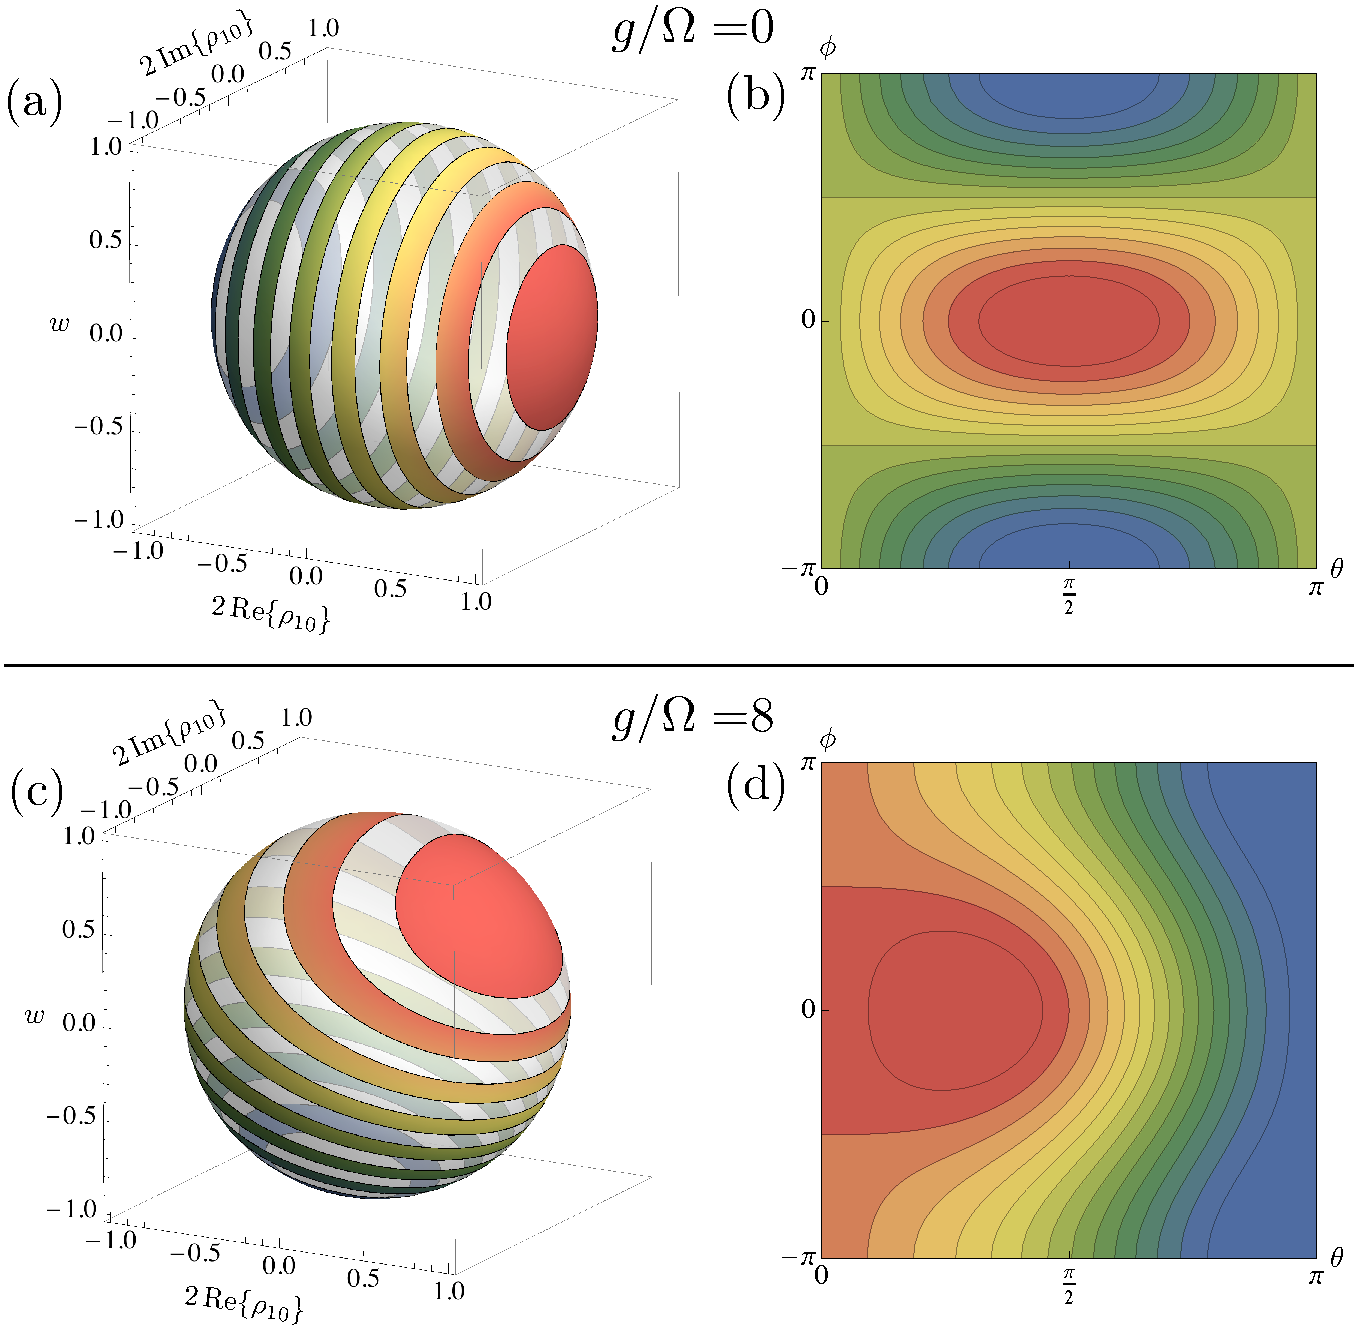
\includegraphics[width=13cm]{BlochSpheres}
    \caption{Bloch sphere representation of the evolution described by \eqref{Peaks:OpticalBlochEquations}. The upper figures (a) and (b) represent the case of the usual optical Bloch equations with no damping ($g/\Omega=0$), middle figures (c) and (d) illustrate the effect of the nonlinear term on the evolution with $g/\Omega = 8$, and the lower figures (e) and (f) illustrate the limit where the nonlinear term dominates ($g/\Omega \rightarrow \infty$). The left figures (a), (c), (e) illustrate the Bloch sphere coloured according to the energy per particle $E$ [see~\eqref{Peaks:OpticalBlochEnergy}]. The system is constrained to move on lines of constant colour. Bands have been removed from these spheres for illustration purposes only. The right figures (b), (d), (f) are contour plots of the energy per particle $E$ over the surface of the Bloch sphere.
     \label{Peaks:BlochSphere}}
\end{figure}

\subsection{Excitation dynamics}

The evolution of small perturbations about the mean-field dynamics of a condensate define both the excitation spectrum of the condensate and its stability to perturbations. 
%These perturbations not only arise from experimental uncertainties, but are an  inescapable consequence of quantum mechanics due to the fluctuations of the vacuum itself.
To determine the evolution of these excitations the mean-field dynamics must be separated from that of the excitations. To this aim we define the deviation operators $\delta\hat{\Psi}_i = \hat{\Psi}_i - \mean{\hat{\Psi}_i}$ and treat $\delta\hat{\Psi}_i$ as a small quantity. In this case the $\mean{\hat{\Psi}_i}=\Psi_i$ are themselves time dependent, obeying the equations for the mean-field \eqref{Peaks:MeanFieldEquationsOfMotion}.

The equations of motion for the deviation operators are obtained by replacing the field operators $\hat{\Psi}_i$ in the operator evolution equations \eqref{Peaks:OperatorEquationsOfMotion} with $\Psi_i + \delta \hat{\Psi}_i$ and keeping only terms up to first order in the deviation operators. Applying this procedure gives
\begin{subequations}
    \label{Peaks:DeviationOperatorsEvolutionXSpace}
    \begin{align}
        \begin{split}
            i \hbar \frac{\partial }{\partial t}\delta \hat{\Psi}_1 =& U\left[ \left(2\abs{\Psi_1}^2+\abs{\Psi_0}^2 \right)\delta \hat{\Psi}_1 + \Psi_1^2\delta\hat{\Psi}_1^\dagger + \Psi_1\Psi_0\delta\hat{\Psi}_0^\dagger + \Psi_0^*\Psi_1\delta\hat{\Psi}_0\right]\\
                    & - \frac{\hbar^2}{2M}\nabla^2 \delta \hat{\Psi}_1 +\hbar \Omega\delta\hat{\Psi}_0- \mu \delta \hat{\Psi}_1,
        \end{split}\\
        \begin{split}
        i \hbar \frac{\partial }{\partial t}\delta \hat{\Psi}_0 =& U\left[\left(2\kappa \abs{\Psi_0}^2 +\abs{\Psi_1}^2\right)\delta\hat{\Psi}_0 + \kappa \Psi_0^2 \delta\hat{\Psi}_0^\dagger + \Psi_1\Psi_0\delta\hat{\Psi}_1^\dagger + \Psi_1^*\Psi_0\delta\hat{\Psi}_1\right]\\
                    & -\frac{\hbar^2}{2M}\nabla^2 \delta \hat{\Psi}_0 +\hbar \Omega\delta\hat{\Psi}_1 - \mu \delta\hat{\Psi}_0.
        \end{split}
    \end{align}
\end{subequations}

Having assumed the mean-field to be homogenous, the evolution equations are spatially translation-invariant and will take their simplest form in a Fourier basis. Performing the Fourier transform of \eqref{Peaks:DeviationOperatorsEvolutionXSpace} yields
\begin{subequations}
    \label{Peaks:DeviationOperatorsEvolutionKSpace}
    \begin{align}
        \begin{split}
            i \hbar \frac{\partial }{\partial t}\delta \hat{\Psi}_1(\bm{k}) =& U\left[ \left(2\abs{\Psi_1}^2+\abs{\Psi_0}^2 \right)\delta \hat{\Psi}_1(\bm{k}) + \Psi_1^2\delta\hat{\Psi}_1^\dagger(-\bm{k}) + \Psi_1\Psi_0\delta\hat{\Psi}_0^\dagger(-\bm{k}) + \Psi_0^*\Psi_1\delta\hat{\Psi}_0(\bm{k})\right]\\
                    & +\frac{\hbar^2 \bm{k}^2}{2M} \delta \hat{\Psi}_1(\bm{k}) +\hbar \Omega\delta\hat{\Psi}_0(\bm{k})- \mu \delta \hat{\Psi}_1(\bm{k}),
        \end{split}\\
        \begin{split}
        i \hbar \frac{\partial}{\partial t} \delta \hat{\Psi}_0(\bm{k}) =& U\left[\left(2\kappa \abs{\Psi_0}^2 +\abs{\Psi_1}^2\right)\delta\hat{\Psi}_0(\bm{k}) + \kappa \Psi_0^2 \delta\hat{\Psi}_0^\dagger(-\bm{k}) + \Psi_1\Psi_0\delta\hat{\Psi}_1^\dagger(-\bm{k}) + \Psi_1^*\Psi_0\delta\hat{\Psi}_1(\bm{k})\right]\\
                    & +\frac{\hbar^2 \bm{k}^2}{2M} \delta \hat{\Psi}_0(\bm{k}) +\hbar \Omega\delta\hat{\Psi}_1(\bm{k}) - \mu \delta\hat{\Psi}_0(\bm{k}).
        \end{split}
    \end{align}
\end{subequations}

In this form, it is clear that the Fourier modes are almost completely decoupled from each other. Each deviation operator $\delta\hat{\Psi}_i(\bm{k})$ is only coupled to $\left\{\delta\hat{\Psi}_j(\bm{k}),\, \delta\hat{\Psi}_j^\dagger(-\bm{k})\right\}$, with each $\delta\hat{\Psi}_i^\dagger(-\bm{k})$ also only coupled to this same set. This can be exploited to write the equations \eqref{Peaks:DeviationOperatorsEvolutionKSpace} in matrix form as
\begin{align}
    \label{Peaks:DeviationOperatorsMatrixEvolution}
    i \hbar \frac{\partial }{\partial t}\hat{\bm{\Upsilon}}(\bm{k}) &= \mathcal{H}(\bm{k}) \hat{\bm{\Upsilon}}(\bm{k}),
\end{align}
where
\begin{align}
    \hat{\bm{\Upsilon}}(\bm{k}) &= 
    \begin{pmatrix}
        \delta\hat{\Psi}_1(\bm{k}) &
        \delta\hat{\Psi}_1^\dagger(-\bm{k}) &
        \delta\hat{\Psi}_0(\bm{k}) &
        \delta\hat{\Psi}_0^\dagger(-\bm{k})
    \end{pmatrix}^\text{T},\\
    \mathcal{H}(\bm{k}) &= 
    \begin{pmatrix}
        \varepsilon(\bm{k}) + q_{1} - \mu & v_{11} & u_{01} + \hbar \Omega & v_{10}\\
        -v_{11}^* & -\varepsilon(\bm{k}) - q_1 + \mu & -v_{10}^* & -u_{10} - \hbar \Omega\\
        u_{10} + \hbar \Omega & v_{10} & \varepsilon(\bm{k}) + q_0 - \mu & \kappa v_{00}\\
        -v_{10}^* & -u_{01} - \hbar \Omega & -\kappa v_{00}^* & -\varepsilon(\bm{k}) - q_0 + \mu
    \end{pmatrix},\label{Peaks:HMatrix}
\end{align}
and $q_1 = U\left(2\abs{\Psi_1}^2+\abs{\Psi_0}^2\right)$, $q_0 = U\left(2\kappa \abs{\Psi_0}^2 + \abs{\Psi_1}^2\right)$, $u_{ij} = U\Psi_i^*\Psi_j$, $v_{ij} = U\Psi_i\Psi_j$, and $\displaystyle \protect{\varepsilon(\bm{k}) = \frac{\hbar^2 \bm{k}^2}{2M}}$.

Note that the matrix $\mathcal{H}(\bm{k})$ is not the Hamiltonian, but is related to it by \eqref{Peaks:ScriptHRelationshipToHamiltonian}. As a consequence, although it will be shown later that in some circumstances $\mathcal{H}(\bm{k})$ contains complex eigenvalues and is hence not Hermitian, this in no way conflicts with the requirement that the Hamiltonian $\hat{H}$ must be Hermitian and only have real eigenvalues.

If the coefficients of the matrix $\mathcal{H}(\bm{k})$ were not time-dependent, the excitation spectrum of the condensate could simply be obtained from the eigenvalues of $\mathcal{H}(\bm{k})$. Non-zero imaginary components for these eigenvalues would indicate the corresponding mode to be unstable\footnote{This is true independent of the sign of the imaginary component as the eigenvalues come in pairs with opposite imaginary components. A full discussion of this issue is given in \appendixref{FloquetAppendix}.}. Before continuing with the general case of $\kappa \neq 1$, in the next section the limit in which all scattering lengths are equal ($\kappa=1$) will be considered and some familiar results recovered.

\subsection{Excitation spectra in the $\kappa = 1$ limit}
\label{Peaks:Kappa1Limit}
In the limit that all the scattering lengths are the same ($\kappa = 1$), the nonlinear term in \eqref{Peaks:MeanFieldEquationsOfMotion} only contributes to a rotation of the global phase of the spinor condensate. In this case the dynamics can be solved analytically and familiar excitation spectra recovered.

The general solution to \eqref{Peaks:MeanFieldEquationsOfMotion} for $\kappa = 1$ is
\begin{subequations}
    \label{Peaks:Kappa1MeanFieldSolution}
    \begin{align}
        \Psi_1(t) &= \cos(\Omega t) \Phi_+ + \sin(\Omega t) \Phi_-, \\
        \Psi_0(t) &= -i\sin(\Omega t) \Phi_+ + i\cos(\Omega t) \Phi_-,
    \end{align}
\end{subequations}
for some complex constants $\Phi_\pm$, and where the chemical potential $\mu = n U$ has cancelled the global phase rotation. This solution can be viewed as a linear basis transformation from $\hat{\Psi}_i$ to $\hat{\Phi}_\pm$, which are the eigenvectors of the Rabi coupling term in \eqref{Peaks:InitialHamiltonian}. Performing this change of basis on the original Hamiltonian \eqref{Peaks:InitialHamiltonian} yields a Hamiltonian of the same form, but without the Rabi coupling term. The equations of motion for the deviation operators $\delta\hat{\Phi}_\pm$ therefore give a matrix of precisely the same form as \eqref{Peaks:HMatrix} but in terms of $\Phi_\pm$ and $\delta\hat{\Phi}_\pm$ instead of the $\Psi_i$ and $\delta\hat{\Psi}_i$, and with $\Omega$ replaced by 0. This new matrix $\mathcal{H}'(\bm{k})$ is time-independent and can be diagonalised to give the eigenvalues
\begin{subequations}
    \label{Peaks:Kappa1Eigenvalues}
    \begin{align}
        \hbar \omega_\uparrow(\bm{k}) &= \sqrt{\varepsilon(\bm{k})\left(\varepsilon(\bm{k}) + 2 n U\right)},\\
        \hbar \omega_\downarrow(\bm{k}) &= \varepsilon(\bm{k}),
    \end{align}
\end{subequations}
where $\displaystyle\varepsilon(\bm{k}) = \frac{\hbar^2\bm{k}^2}{2M}$, $n= \abs{\Psi_1}^2 + \abs{\Psi_0}^2$ and the remaining two eigenvalues are the negatives of \eqref{Peaks:Kappa1Eigenvalues}. $\hbar \omega_\uparrow(\bm{k})$ is the usual Bogoliubov spectrum \citep{Bogoliubov:1947} corresponding to excitations in the total condensate density. The eigenvalue $\hbar \omega_\downarrow(\bm{k})$ is the free particle spectrum; this excitation only changes the relative densities of the two states without affecting the total density, hence not affecting the nonlinear term in the Hamiltonian \eqref{Peaks:InitialHamiltonian}.

The Hamiltonian for the condensate excitations that corresponds to the eigenvalues \eqref{Peaks:Kappa1Eigenvalues} is (refer to \sectionref{Peaks:ElementaryExcitations})
\begin{align}
    \hat{H} &= \sum_{i=\uparrow,\downarrow}\int d\bm{k}\, \hbar \omega_i(\bm{k}) \hat{\Lambda}_i^\dagger(\bm{k}) \hat{\Lambda}_i^{\phantom{\dagger}}(\bm{k}),
\end{align}
where the $\hat{\Lambda}_{\uparrow,\downarrow}(\bm{k})$ obey boson commutation relations and are the corresponding normalised eigenvectors to the eigenvalues in \eqref{Peaks:Kappa1Eigenvalues}. The normalised eigenvectors for the negatives of those eigenvalues are the $\hat{\Lambda}_{\uparrow, \downarrow}^\dagger(-\bm{k})$.

\subsection[Floquet's theorem]{Floquet's theorem \citep[\S 3.2]{AppliedNonlinearDynamics}}
\label{Peaks:FloquetsTheorem}

Having considered the limit of equal scattering lengths, it now remains to determine the energy spectrum and condensate stability in the general case of $\kappa \neq 1$. Analytic results cannot be obtained in this limit, but numeric results corresponding to the experimental situation in \sectionref{Peaks:ExperimentalSetup} can be obtained.

In the general case, the excitation spectrum cannot be obtained from the eigenvalues of the matrix $\mathcal{H}(\bm{k})$ in \eqref{Peaks:HMatrix} as the matrix's entries are themselves time-dependent. However, due to the periodicity of the mean-field wavefunctions demonstrated in \sectionref{Peaks:MeanFieldPeriodicity}, the entries of $\mathcal{H}(\bm{k})$ are themselves periodic, which enables Floquet's theorem to be applied.

Floquet's theorem proves that the matrix solution to the initial-value problem
\begin{subequations}
    \label{Peaks:FloquetMatrixIVP}
    \begin{align}
        \frac{d}{dt}\bm{\Pi}(t) &= \bm{A}(t) \bm{\Pi}(t),\\
        \bm{\Pi}(0) &= \mathbb{I},
    \end{align}
\end{subequations}
where $\mathbb{I}$ is the $n \times n$ identity matrix and $\bm{A}(t)$ a periodic $n \times n$ matrix with period $T$ can be written in the form
\begin{align}
    \bm{\Pi}(t) = \bm{P}(t) \exp(-i\bm{Q} t),
    \label{Peaks:FloquetSolution}
\end{align}
for some constant matrix\footnote{There are differing definitions of the matrix $\bm{Q}$. While it is usual in quantum mechanics literature \citep{Shirley:1965,Hanggi:1998,Garrison:1999} to define \eqref{Peaks:FloquetSolution} with the $-i$ in the exponent,  in mathematics literature \citep{Moulton:1958,AppliedNonlinearDynamics} the $-i$ is omitted.} $\bm{Q}$ and $\bm{P}(t)$ a matrix of periodic functions with period $T$ and $\bm{P}(0) = \mathbb{I}$. The matrix solution $\bm{\Pi}(t)$ is the general solution to the related linear system
\begin{align}
    \frac{d}{dt}\bm{x}(t) &= \bm{A}(t) \bm{x}(t),
    \label{Peaks:FloquetVectorIVP}
\end{align}
for any initial condition $\bm{x}(0)$ where $\bm{x}(t)$ is a vector. Every solution $\bm{x}(t)$ to this problem can be written in terms of the matrix $\bm{\Pi}(t)$ as
\begin{align}
    \bm{x}(t) &= \bm{\Pi}(t) \bm{x}(0),
\end{align}
as is easily verified. The matrix solution $\bm{\Pi}(t)$ thus completely determines the behaviour of all solutions to \eqref{Peaks:FloquetVectorIVP}.

The eigenvalues of $\bm{Q}$ are known as \emph{Floquet exponents} (or \emph{characteristic exponents}) and determine the long-term growth or decay of the solutions to \eqref{Peaks:FloquetVectorIVP}. These eigenvalues can be obtained from the \emph{monodromy matrix},
\begin{align}
    \label{Peaks:MonodromyMatrix}
    \mathcal{M} &= \bm{\Pi}(T) = \exp(-i\bm{Q} T),
\end{align}
as $\bm{P}(T) = \bm{P}(0) = \mathbb{I}$. The existence and uniqueness of the solution to \eqref{Peaks:FloquetMatrixIVP} guarantees that $\bm{\Pi}(t)$ and hence $\mathcal{M}$ will be invertible. The Floquet exponents $\xi_i$ can therefore be obtained from the eigenvalues $\lambda_i$ of the monodromy matrix using $\lambda_i = \exp(-i\xi_i T)$.\footnote{Note that the Floquet exponents are only defined modulo $2 \pi/T$ as $\displaystyle\lambda = \exp(-i\xi T) = \exp\left[-i \left(\xi + n \frac{2 \pi}{T}\right)T\right]$ for any integer $n$.} It is the Floquet exponents of the matrix $\mathcal{H}(\bm{k})$ that we wish to calculate in order to determine the stability of the condensate to excitations.

\subsection{Determination of the dynamical instabilities}
\label{Peaks:ExperimentEigenvalues}

The method outlined in the previous section for determining the Floquet exponents of the system \eqref{Peaks:DeviationOperatorsMatrixEvolution} requires knowledge of its period $T$, and hence the period of the mean field dynamics given by \eqref{Peaks:MeanFieldEquationsOfMotion}. Although this period cannot be determined analytically, it can be found numerically.

It was shown in \sectionref{Peaks:MeanFieldPeriodicity} that up to a global phase rotation $\displaystyle f(T) = e^{i 2\pi \Delta \nu T}f(0)$, the mean fields $\Psi_j(t)$ are periodic. The mean fields $\Psi_j(t)$ can be therefore written in the form
\begin{align}
    \label{Peaks:MeanFieldFourierDecomposition}
    \Psi_j(t) = \sum_{n=-\infty}^\infty \alpha_{j,n} \exp\left[i 2\pi \left( n \nu_0 + \Delta\nu\right)t \right],
\end{align}
for some complex constants $\alpha_{j, n}$, fundamental frequency $\nu_0 = T^{-1}$, and frequency offset $\Delta \nu$. In this form, the $\Psi_j(t)$ are not exactly periodic as $\Psi_j(T) = \exp(i\Delta \nu T)\Psi_j(0)$, but this frequency offset can be cancelled by an appropriate choice of the energy offset $\mu = 2\pi\hbar \Delta \nu$ in \eqref{Peaks:InitialHamiltonian}.

The period $T$ and frequency offset $\Delta\nu$ in \eqref{Peaks:MeanFieldFourierDecomposition} can be determined from the Fourier transform of $\Psi_j(t)$, which will have sharp peaks at the frequencies $n \nu_0 + \Delta \nu$ (see \figureref{Peaks:MeanFieldFourierTransform}). Choosing the energy offset $\mu=-h \nu$, the frequency offset in \eqref{Peaks:MeanFieldFourierDecomposition} can be cancelled making the $\Psi_j(t)$ with this energy offset exactly periodic with period $T$. \figureref{Peaks:MeanFieldFourierTransform} illustrates the Fourier transform of the numerical solutions for $\Psi_j(t)$ for a Rabi frequency of $\Omega = 2 \pi \times \unit[3]{kHz}$ from which the period $T=\unit[150]{\micro{}s}$ and frequency offset $\Delta \nu = \unit[-1.78]{kHz}$ have been obtained.

\begin{figure}
    \centering
    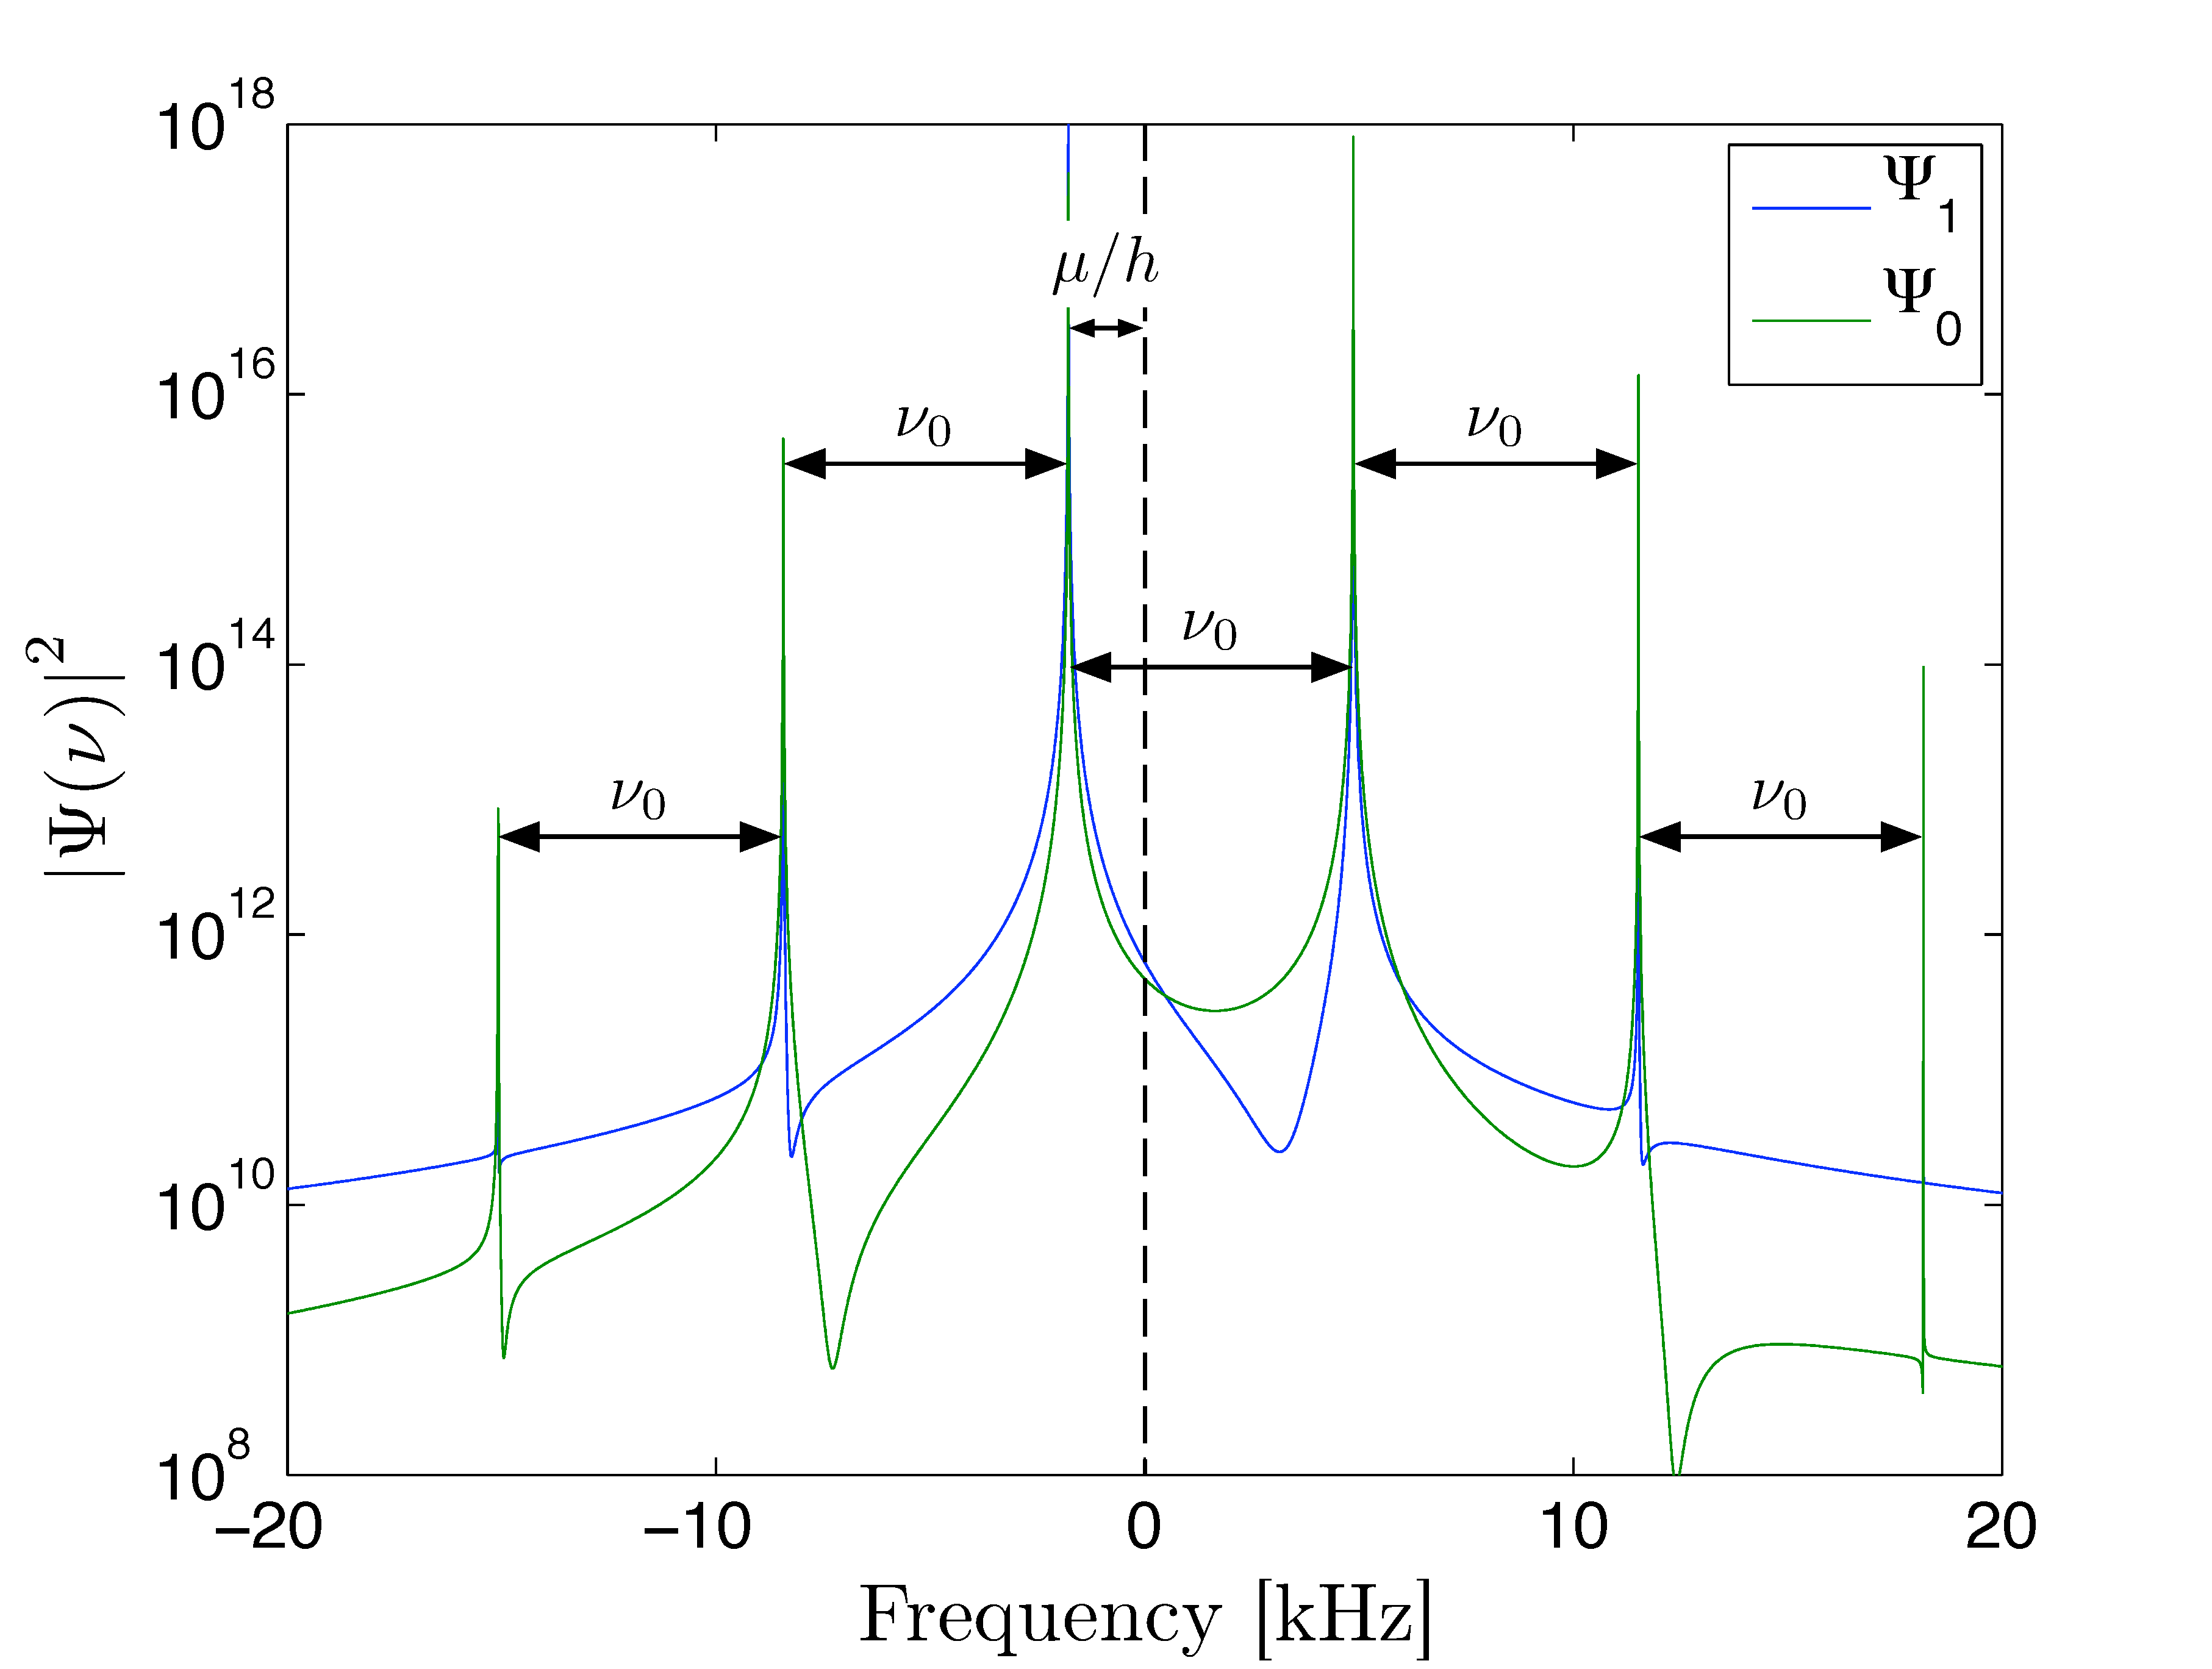
\includegraphics[width=14cm]{MeanFieldFourierTransform}
    \caption{Temporal Fourier transform of the calculated mean field evolution defined by \eqref{Peaks:MeanFieldEquationsOfMotion} for the centre of the condensate defined by the experimental parameters given in \tableref{Peaks:ExperimentalParameters}. The frequency $\nu_0$ is the inverse period of the system, and $\Delta\nu$ represents the global phase rotation. From the data in this figure the values $\nu_0 = \unit[6.65]{kHz}$ and $\Delta\nu = \unit[-1.78]{kHz}$ can be determined, giving the period as $T=\unit[150]{\micro{}s}$. \label{Peaks:MeanFieldFourierTransform}}
\end{figure}

The period and energy offset determined, it remains to calculate the mono\-dromy matrix $\mathcal{M}(\bm{k})$ from which the Floquet exponents may be derived. This is achieved by numerically solving the related matrix problem to \eqref{Peaks:DeviationOperatorsMatrixEvolution} from $t=0$ to $t=T$ [refer to \eqref{Peaks:MonodromyMatrix}]. Noting that the matrix $\mathcal{H}(\bm{k})$ only depends on $k = \abs{\bm{k}}$, the solutions for the Floquet exponents $\xi(\bm{k}) = \omega(\bm{k}) + i\gamma(\bm{k})$ are illustrated in \figureref{Peaks:CondensateEigenvalues}.

In the limit that the mean-field is time-independent (a degenerate case of periodicity), the Floquet exponents $\xi(\bm{k})$ are related to the eigenvalues $\lambda(\bm{k})$ of the matrix $\mathcal{H}$ by $\xi(\bm{k}) = \frac{1}{\hbar} \lambda(\bm{k})$. It was previously stated that eigenvalues of $\mathcal{H}(\bm{k})$ with nonzero imaginary components would be unstable, this is therefore also true for the Floquet exponent $\xi(\bm{k})$.

\begin{figure}
    \centering
    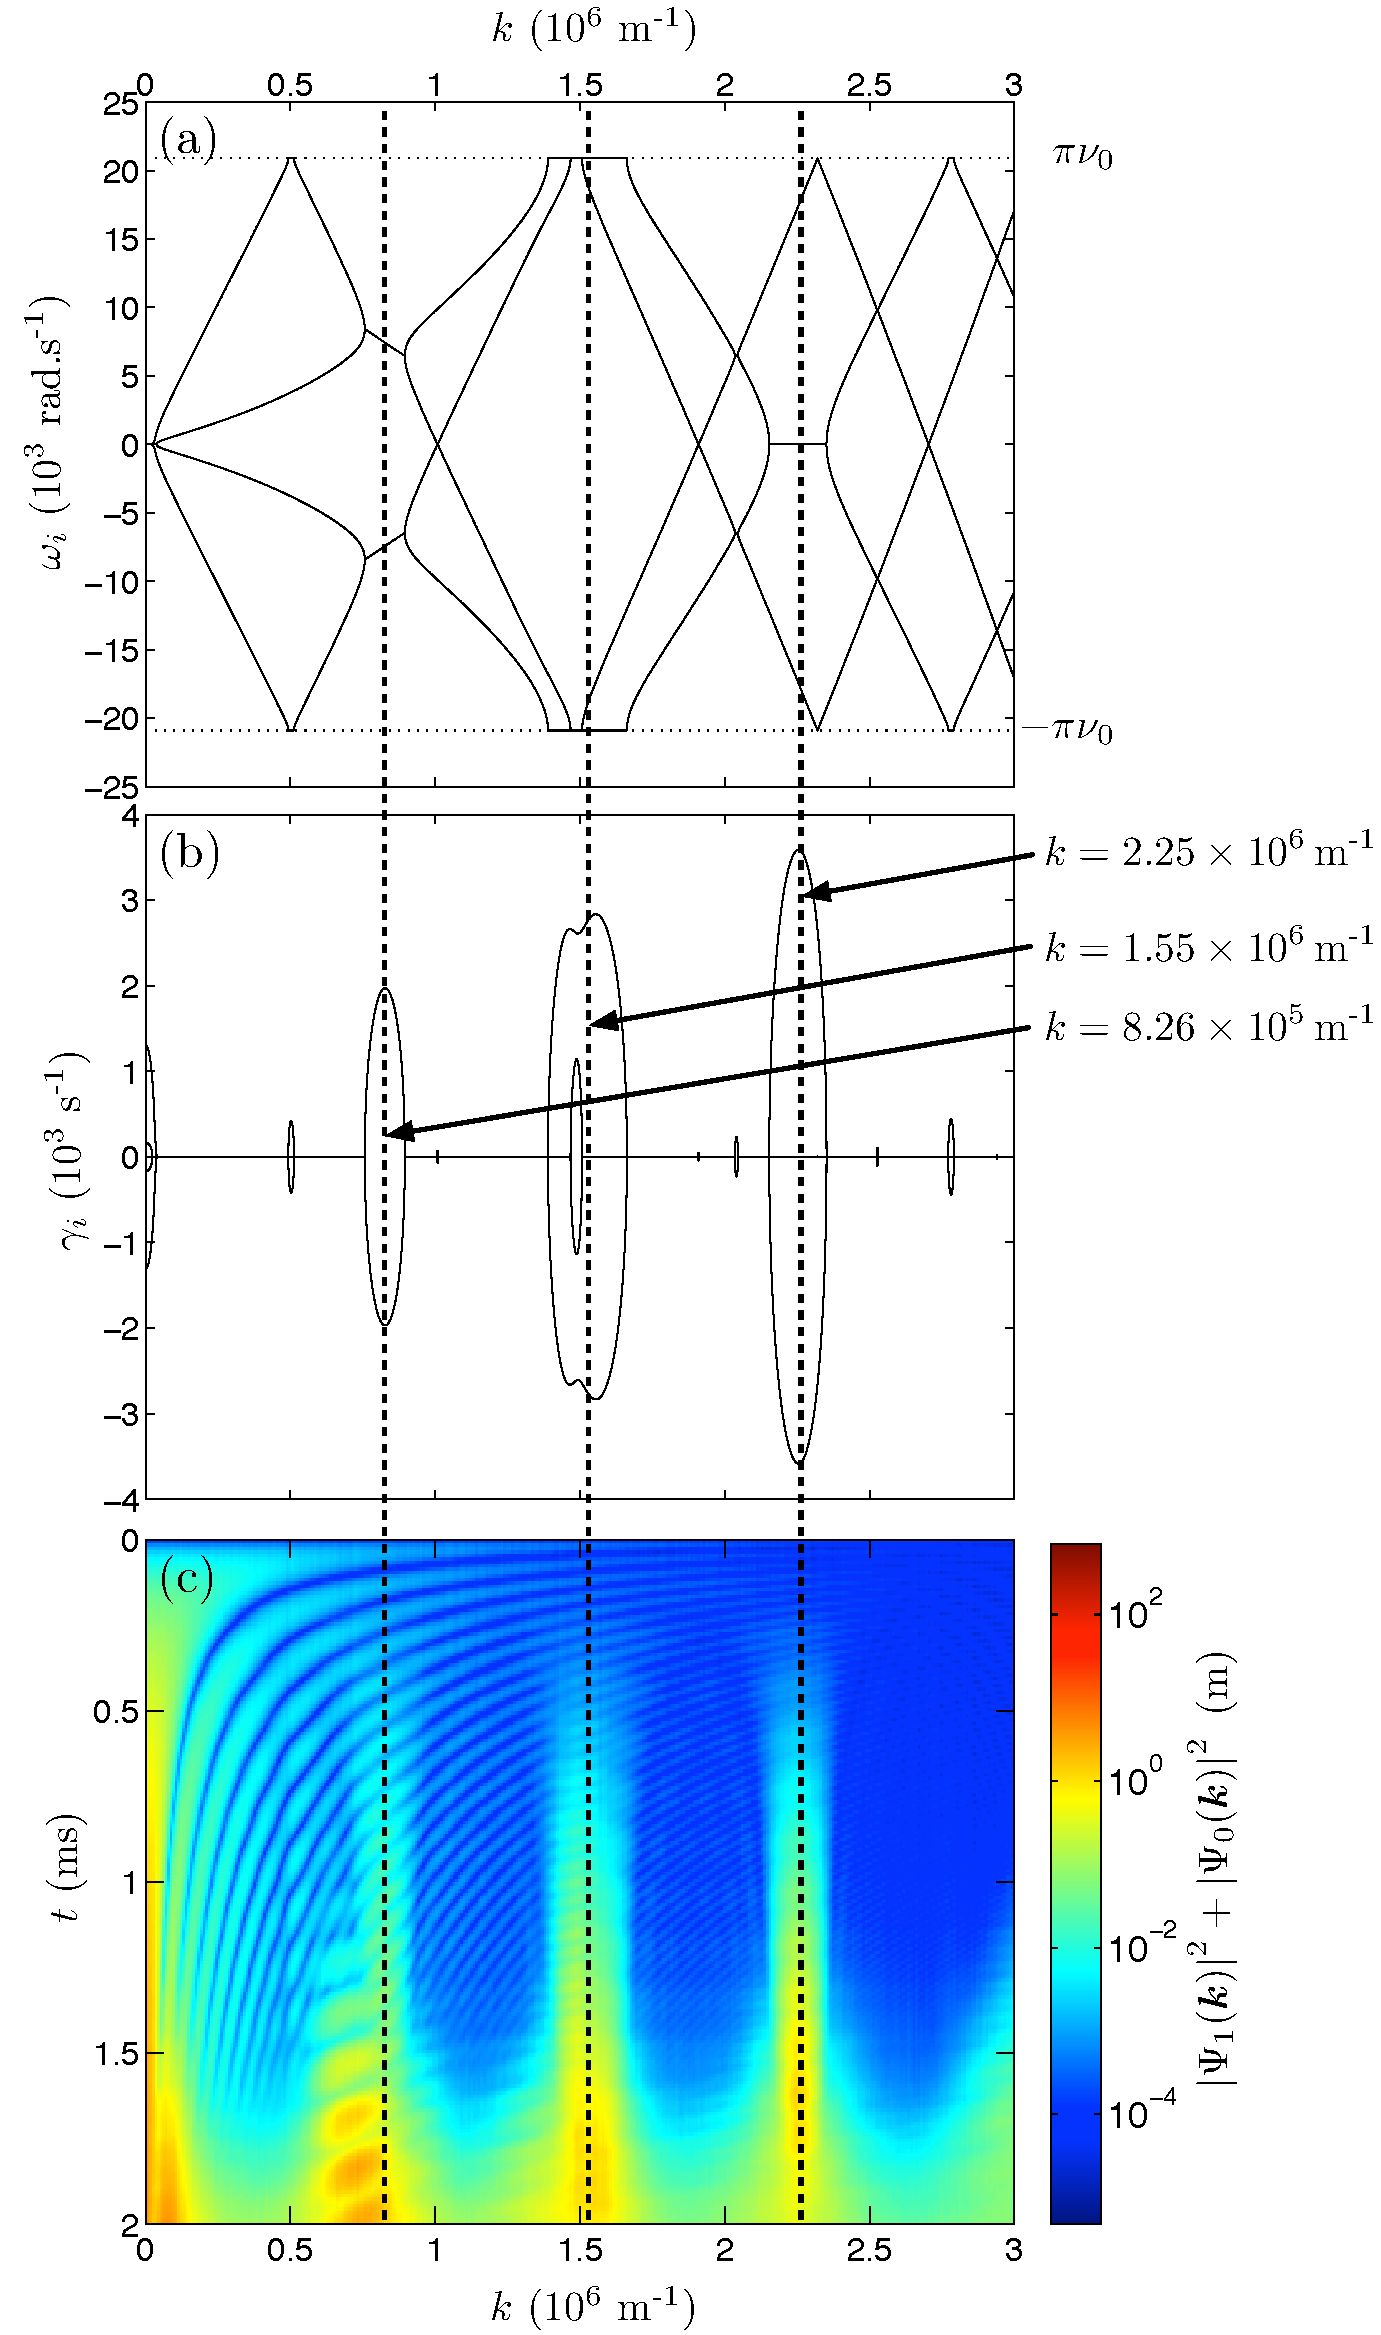
\includegraphics[height=19cm]{CondensateEigenvalues}
    \caption{Illustration of the Floquet exponents for $\mathcal{H}(\bm{k})$ and comparison to a corresponding truncated Wigner simulation for $\Omega = 2\pi \times \unit[3]{kHz}$.
        Upper figure (a) displays the imaginary part $\omega_i$ of the Floquet exponents. As the $\omega_i$ can only be determined up to a multiple of $2\pi\nu_0$ [see \eqref{Peaks:AmbiguityFloquetExponent}], they have been reduced modulo $2\pi\nu_0$ into the range $\left[-\pi\nu_0,\, \pi\nu_0\right]$.
        The middle figure (b) shows the real part $\gamma_i$ of the Floquet exponents, which indicate an instability for the corresponding wavenumber when they are nonzero.
        Lower figure (c) shows the results of a 1D truncated Wigner simulation corresponding to the system under consideration in (a) and (b). The truncated Wigner simulation exhibits growth in the same modes predicted from the results of the perturbative analysis shown in (b). The truncated Wigner results shown are the average of 500 realisations.
        \label{Peaks:CondensateEigenvalues}}
\end{figure}

The temporal periodicity of the system implies that the real components $\omega_i(\bm{k})$ of the Floquet exponents are only uniquely defined modulo $2\pi \nu_0$ (see \figureref{Peaks:CondensateEigenvalues}(a)). This is because any eigenvalue $\lambda$ of the monodromy matrix $\mathcal{M}(\bm{k})$ corresponds to infinitely many Floquet exponents,
\begin{align}
    \label{Peaks:AmbiguityFloquetExponent}
    \lambda = \exp\left[-i \left(\omega + 2 \pi n \nu_0 + i \gamma\right)T\right] = \exp\left[-i\left(\omega + i \gamma\right)T\right].
\end{align}
This does not hinder our understanding of the system as our primary interest is in the stability of the condensate to excitations, which is determined by the $\gamma_i(\bm{k})$.

The normalised eigenvectors of the system are not always annihilation or creation operators; as is discussed in \appendixref{FloquetAppendix}, this is only true when the Floquet exponents are purely real. When the Floquet exponents have a nonzero imaginary component, annihilation and creation operators can be constructed from linear combinations of the eigenvectors. Not being eigenvectors, these operators will therefore have nontrivial evolution. As is shown in \appendixref{FloquetAppendix}, Floquet exponents with nonzero imaginary parts come in pairs of the form $\pm \gamma(\bm{k}) + i \omega(\bm{k})$. From the corresponding eigenvectors to these Floquet exponents the bosonic annihilation operator $\hat{\Lambda}(\bm{k}, t)$ can be formed, which evolves as
\begin{subequations}
    \label{Peaks:DynamicalInstability}
    \begin{align}
        \hat{\Lambda}(\bm{k}, nT) &= e^{i n\omega(\bm{k}) T} \left( \sinh(n\gamma(\bm{k}) T) \hat{\Lambda}'^\dagger(-\bm{k}, 0) + \cosh(n\gamma(\bm{k}) T) \hat{\Lambda}(\bm{k}, 0)\right),\\
        \hat{\Lambda}'(\bm{k}, nT) &= e^{-i n \omega(\bm{k}) T} \left( \sinh(n\gamma(\bm{k}) T) \hat{\Lambda}^\dagger(-\bm{k}, 0) + \cosh(n\gamma(\bm{k}) T) \hat{\Lambda}'(\bm{k}, 0)\right),
    \end{align}
\end{subequations}
where $n$ is a positive integer, and where $\hat{\Lambda}'(\bm{k}, t)$ will be equal to $\hat{\Lambda}(\bm{k}, t)$ in some circumstances as discussed in \appendixref{FloquetAppendix}. Due to the exponential growth in \eqref{Peaks:DynamicalInstability}, the mode corresponding to $\hat{\Lambda}(\bm{k})$ represents a dynamical instability of the condensate.

The behaviour of the dynamical instabilities will be governed by \eqref{Peaks:DynamicalInstability} only while the unstable modes have a small occupation compared to the condensate, and scattering between the unstable modes can be neglected. \figureref{Peaks:CondensateEigenvalues}(c) shows the results of a truncated Wigner simulation of the Hamiltonian \eqref{Peaks:InitialHamiltonian}, which is in excellent agreement with the location of the dynamical instabilities as determined by the Floquet exponents [see \figureref{Peaks:CondensateEigenvalues}(b)]. For later times, there is an additional mode undergoing growth, $k \approx \unit[7.5\times 10^5]{m}^{-1}$. This mode is the result of scattering between the dynamical instabilities, a process neglected the perturbative approach taken in this section. 

\parasep

In summary, the procedure used to find the Floquet exponents of $\mathcal{H}(\bm{k})$, and hence the stability of the condensate to excitations is:
\begin{enumerate}
    \item Numerically solve \eqref{Peaks:MeanFieldEquationsOfMotion} with $\mu=0$ for a long period of time $t \gg T$ where $T$ is the periodicity of the solution.
    \item Perform the temporal Fourier transform of the solutions obtained for $\Psi_i(t)$ to accurately determine the period $T$ and the value of the energy offset $\mu$ required to cancel any global phase evolution to make the wavefunctions themselves periodic (see \figureref{Peaks:MeanFieldFourierTransform}).
    \item Using the calculated period and energy offset, numerically solve the related matrix problem to \eqref{Peaks:DeviationOperatorsMatrixEvolution} for a range of values of $\bm{k}$ to obtain the monodromy matrix $\mathcal{M}(\bm{k})$. In this calculation the matrix $\bm{A}(t)$ in \eqref{Peaks:FloquetMatrixIVP} is $\displaystyle -\frac{i}{\hbar}\mathcal{H}(\bm{k}, t)$.
    \item Calculate the eigenvalues $\lambda_i$ of $\mathcal{M}(\bm{k})$ and determine the Floquet exponents $\xi_i$ using $\protect{\lambda_i = \exp(-i \xi_i T)}$ (see \figureref{Peaks:CondensateEigenvalues}). The real parts of these Floquet exponents gives the energy spectrum, with nonzero imaginary parts giving the growth rate for the corresponding instability.
\end{enumerate}

\subsection{Discussion of the dynamical instabilities}
\label{Peaks:DynamicalInstabilitiesDiscussion}

The dynamics of the dynamical instability $\hat{\Lambda}(\bm{k})$ described by \eqref{Peaks:DynamicalInstability} are the same as those of the amplified modes in non-degenerate parametric down-conversion \citep{WallsMilburn}.  In parametric down-conversion, a non-linear crystal produces pairs of EPR-entangled\footnote{EPR entanglement was proposed by Einstein, Podolsky and Rosen \citep{Einstein:1935} as a demonstration that quantum mechanics could not simultaneously be local, real and complete.  Their preferred option of local and real but \emph{incomplete} has since been demonstrated to be incorrect \citep{Aspect:1982uq}.  For more information about EPR entanglement, see \citep[Chapter 18]{Scully}.} photons at frequencies $\omega_1$ and $\omega_2$ from a classical seed beam at frequency $\omega = \omega_1 + \omega_2$.  Analogously, in the case of the He* BEC discussed at the start of this chapter, the evolution represented by \eqref{Peaks:DynamicalInstability} will result in the spontaneous formation of EPR-entangled pairs of excitations, one in each of the $\hat{\Lambda}(\pm \bm{k})$ modes. Although these modes will be entangled upon production, it does not necessarily follow that parts of the outcoupled atom laser will be entangled; the entangled $\hat{\Lambda}(\bm{k})$ modes are each superpositions of $m_F=1$ and $m_F=0$ states, but only the $m_F=0$ atoms can leave the condensate. However, if the $m_F=1$ components of the entangled modes are outcoupled faster than the time to reverse their momenta ($\unit[9]{ms}$), then number difference squeezing between the atom laser components with opposite axial momenta may be observed.

The unstable excitations would not necessarily be expected to form along the tight trapping directions. Of the three most unstable modes in \figureref{Peaks:CondensateEigenvalues}, the shortest wavelength for these excitations is $\lambda \approx \unit[3]{\micro m}$ which is not significantly smaller than the Thomas-Fermi radius in this dimension of $\rho_\text{TF} = \unit[9.4]{\micro m}$. Hence the local density approximation will not be satisfied in this dimension as the condensate density decays to zero over a distance a few times larger than the size of the excitation itself.  However, as the Thomas-Fermi radius in the axial dimension is $z_\text{TF} = \unit[175]{\micro m}$, the local density approximation will be a good approximation for describing the excitations along that dimension. Therefore excitations should form along the axial dimension.

This effect also depends on the scattering length for collisions between $m_F=0$ atoms being significantly smaller than both the 1--1 and 1--0 scattering lengths as no instabilities were found in the $\kappa = 1$ limit (see \sectionref{Peaks:Kappa1Limit}). 
Consequently, this effect would not be expected to be observed in atoms like $\nucl{87}{}{Rb}$ for which $\kappa = 1.002$ \citep{Kempen:2002,Widera:2006}.

Verification that the $\hat{\Lambda}(\bm{k})$ quasiparticles are the origin of the peak-like structure observed in the experiment required a full 3D field calculation, which is discussed in \sectionref{Peaks:3DCalculation}.  The argument made in this section that the observed structure is due to the formation of pairs of quasiparticles driven by a spontaneous four-wave mixing process indicates that a Gross-Pitaevskii model will be unable to reproduce the observations. Such a mean-field model will be insufficient due to the absence of the vacuum fluctuations which are critical to all spontaneous processes.

\section{Full 3D calculation}
\label{Peaks:3DCalculation}
In the previous section it was found that the process of outcoupling from the He* BEC discussed in \sectionref{Peaks:ExperimentalSetup} results in certain modes within the condensate becoming unstable. It was argued that these instabilities are the original cause of the observed structure in \figureref{Peaks:ExperimentalResults}. However, it is not immediately clear that these instabilities will not be suppressed by Penning ionisation which causes $m_F=0$ atoms to ionise but not pure samples of $m_F=1$ atoms (see \sectionref{BackgroundTheory:PenningIonisation} and \appendixref{PenningIonisationAppendix}). To verify that the instabilities are not suppressed and that they do cause the observed structure, a detailed numerical simulation of the experiment was performed.

The master equation that describes the experiment described in \sectionref{Peaks:ExperimentalSetup} is given by
\begin{align}
    \label{Peaks:MasterEquation}
    \frac{d }{d t}\hat{\rho} &= \frac{-i}{\hbar} [\hat{H},\, \hat{\rho} ] + \frac{9}{2} K^\text{(unpol)}_{^{4}\text{He}} \int d \bm{x}\, \mathcal{D}\left[\hat{\Xi}_{S=0,m_S=0} \right] \hat{\rho},
\end{align}
where $\displaystyle\hat{\Xi}_{S, m_S}$ is the annihilation operator for the quasimolecular state with total hyperfine spin $S$ and projection $m_S$, $\mathcal{D}[\hat{c}]\hat{\rho} \equiv \hat{c}\hat{\rho}\hat{c}^\dagger - \frac{1}{2}(\hat{c}^\dagger \hat{c} \hat{\rho} + \hat{\rho} \hat{c}^\dagger \hat{c})$ is the usual decoherence superoperator, and the second term\footnote{The reason for the difference between the ${54}/{5}$ factor in \citet{Dall:2009} and the $9/2$ factor in \eqref{Peaks:MasterEquation} is a difference of a factor of $\sqrt{2}$ in the definition of $\hat{\Psi}_{J=0}^{\text{(mol)}}$ in \citep{Dall:2009} and $\displaystyle\hat{\Xi}_\ket{S=0, m_S=0}$ here, and a calculational error of the order of 20\% in \citep{Dall:2009}.} on the RHS in \eqref{Peaks:MasterEquation} is due to Penning ionisation (refer to \sectionref{BackgroundTheory:PenningIonisation} and \appendixref{PenningIonisationAppendix}) with $K^\text{(unpol)}_{^{4}\text{He}}=\unit[7.7\times 10^{-17}]{m\textsuperscript{3}s\textsuperscript{-1}}$ the Penning ionisation rate for an unpolarised thermal sample of He* \citep{Stas:2006kx}. The Hamiltonian in \eqref{Peaks:MasterEquation} is given by
\begin{align}
    \label{Peaks:3DHamiltonian}
    \begin{split}
    \hat{H} &= \sum_i \int d\bm{x}\, \hat{\Psi}_i^\dagger \left(\frac{-\hbar^2 \nabla^2}{2 M} + V_i(\bm{x})\right)\hat{\Psi}_i^{\phantom{\dagger}} + \sum_{S, m_S} g_{S}\int d\bm{x}\, \hat{\Xi}_{S, m_S}^\dagger \hat{\Xi}_{S, m_S}^{\phantom{\dagger}}\\
    \\
            &\phantom{=} + \sqrt{2} \hbar \Omega \sum_{i j}\int d\bm{x}\, \hat{\Psi}_i^\dagger \left(\delta_{i, j+1} + \delta_{i, j-1}\right) \hat{\Psi}_j^{\phantom{\dagger}},
    \end{split}
\end{align}
$\displaystyle \hat{\Psi}_i$ is the annihilation operator for the atomic state $\displaystyle \ket{F=1, m_F=i}$, $V_i(\bm{x})$ is the potential experienced by that state, and $g_S = 4 \pi \hbar^2 a_S/M$ is the nonlinear interaction strength, and $a_S$ is the $s$-wave scattering length for the total hyperfine spin $S$ channel (refer to \sectionref{BackgroundTheory:Helium}). The quasimolecular annihilation operator $\displaystyle \hat{\Xi}_{S, m_S}$ is defined in terms of the atomic annihilation operators and the appropriate Clebsch-Gordan coefficients \citep{Ho:1998}. For example $\displaystyle \hat{\Xi}_{S=0, m_S=0} = \frac{1}{\sqrt{3}} \left( 2 \hat{\Psi}_1 \hat{\Psi}_{-1} - \hat{\Psi}_0 \hat{\Psi}_0\right)$.

In the first instance, we wish to verify the results of the previous section within a fully three-dimensional model and determine the pattern that would be observed on the detector in this case. Although a similar system was solved with the GP equation in \sectionref{TransverseProfile:Helium} when the transverse profile of a He* atom laser was considered, it is not possible to solve the system corresponding to \eqref{Peaks:MasterEquation} with available computational infrastructure. The difference between these two systems is in the axial dimension.

When modelling the transverse profile of the atom laser, the tight aspect ratio of the condensate meant that outcoupled atoms would be accelerated much more along the radial trapping directions than along the axial trapping direction. This permitted the use of a much larger spatial grid separation in the axial dimension than in the radial dimensions. In the present system it is expected that there will exist instabilities with momenta that correspond to a substantial fraction of that which the atom laser would have after leaving the condensate ($\sim \unit[2 \times 10^6]{m\textsuperscript{-1}}$ as compared to $\sim \unit[4 \times 10^6]{m\textsuperscript{-1}}$). In the present case the spatial grid separation in the axial dimension must be comparable to that used in the radial dimensions. Exacerbating this problem is that the tighter aspect ratio in the experiment described in this chapter requires this significantly smaller spatial grid separation be used over a larger range. To perform a simulation using a method similar to that used in \sectionref{TransverseProfile:Helium}, approximately $\unit[500]{GiB}$ of memory would be needed simply to store the wavefunctions for the system. Additional approximations are necessary to make this system tractable.

One of the most effective ways to reduce the size of a problem is by reducing its dimensionality. Although the master equation \eqref{Peaks:MasterEquation} possesses no continuous symmetries, near the BEC it is approximately cylindrically symmetric. The only term breaking this cylindrical symmetry is the gravitational potential $V_\text{grav}(\bm{x}) =- M \bm{g} \cdot \bm{x}$ where $\bm{g}$ is the gravitational field strength. While this term can be neglected over the region close to the BEC as it varies by only $10\%$ of the chemical potential of the BEC, it certainly cannot be neglected when considering the propagation of the atom laser onto the detector located $\unit[4]{cm}$ below. However, as discussed in \sectionref{TransverseProfile:Helium} the evolution of the atom laser in the region below the BEC is well described by free fall with the exception of fine-scale interference effects. In this chapter it is only the large-scale structure that is of interest, enabling a classical description for the atom laser to be used after it leaves the immediate vicinity of the condensate where the important dynamics will occur.

Another demonstration of the validity of the assumption of cylindrical symmetry is that the gravitational sag of the centre of the condensate from the centre of the trap is only $\unit[0.2]{\micro m}$, which is small compared to the Thomas-Fermi radius in the tight trapping dimensions of $r_\text{TF} = \unit[9.4]{\micro m}$. Consequently, atoms will be repelled from the condensate almost symmetrically. Such a situation was observed earlier in \sectionref{TransverseProfile:Helium}.

To solve the system corresponding to the master equation \eqref{Peaks:MasterEquation}, a two-step method is used. First, the system is modelled either with a GP equation or a Truncated Wigner method in a restricted cylindrical region enclosing the condensate using absorbing boundary layers (see \sectionref{BackgroundTheory:AbsorbingBoundaryLayers}) to prevent the atom laser interacting with the artificial boundary conditions. Second, the momentum density that left the simulation region (calculated using a method described in \sectionref{Peaks:AbsorbingBoundaryTricks}) is then propagated classically to determine the profile on the detector, which is located $\unit[4]{cm}$ below the BEC. This two-step procedure will permit the use of cylindrical symmetry to reduce the dimensionality of the computational domain while still considering the full three-dimensional behaviour of the system.

\subsection{Choice of artificial boundary conditions}

The freedom of choice for the artificial boundary conditions can be used to ensure the accurate calculation of all terms in \eqref{Peaks:MasterEquation} and \eqref{Peaks:3DHamiltonian}. With the exception of the kinetic energy term, all terms in these equations are local in space hence their accurate calculation is guaranteed by any spatial representation. It is appropriate therefore to use the freedom in the choice of the artificial boundary conditions to permit the solution to be equivalently represented as a sum of the eigenfunctions of the kinetic energy operator,
\begin{align}
    \label{Peaks:SpectralRepresentation}
    f(x) &= \sum c_n g_n (x)
\end{align} 
where $f(x)$ is the spatial representation of the solution, $g_n(x)$ are the eigenfunctions of the kinetic energy and hence Laplacian operator, and $\left\{c_n\right\}$ are complex constants which form an equivalent representation of the solution (the \emph{spectral} representation \citep{SpectralMethods}). Equation~\eqref{Peaks:SpectralRepresentation} can be viewed as a change of basis for the solution from the spectral or momentum representation to the spatial representation. This change of basis is invertible as the $g_n(x)$ are orthogonal and complete. For rectangular domains the eigenfunctions $g_n(x)$ are the complex exponentials, which imply periodic boundary conditions. The Fourier transform and its inverse connect the spatial and spectral representations of the solution on this domain.

In this chapter it is desired to make use of the cylindrical symmetry of the system, hence it is appropriate to represent the solution as a sum of the cylindrically-symmetric eigenfunctions of the Laplacian operator: Bessel functions. The artificial boundary conditions implied by the use of Bessel functions are analyticity at the origin, and Dirichlet boundary conditions at the edge of the domain where the solution is zero. The spatial and spectral representations of the solution are connected by the Hankel transform \citep[Chapter 15]{ArfkenWeber} and its inverse. The use of the Bessel basis and the Hankel transform to solve the GP equation is described in \citep{Ronen:2006}.

Although the Bessel basis is arguably a more useful basis for cylindrically-symmetric problems, the choice of boundary conditions is artificial and for the results presented in \citep{Dall:2009} a Fourier basis was used on a domain symmetric about the origin. When using a Fourier basis for cylindrical coordinates, care must be taken due to the form of the Laplacian operator,
\begin{align}
    \nabla^2 u(r, z) &= \left(\frac{\partial^2 }{\partial r^2} + \frac{1}{r}\frac{\partial }{\partial r} + \frac{\partial^2 }{\partial z^2}\right)u(r, z).
\end{align}
In particular, the radial grid must be chosen to exclude the origin due to the apparent divergence in the $r^{-1}$ term in the Laplacian. Note that this is divergence is not real; for sufficiently well-behaved $u(r, z)$, $\nabla^2 u(r, z)$ will be continuous at the origin.

The reason for the choice of the Fourier basis over the Bessel basis in \citep{Dall:2009} was purely practical: the tools available at the time were not capable of using the Bessel basis. As discussed in \appendixref{ToolsAppendix}, this shortcoming has since been rectified and all results presented in this chapter have been calculated using the Bessel basis, but differ negligibly from the results presented in \citep{Dall:2009}.

\subsection{Calculation of the momentum flux density}
\label{Peaks:AbsorbingBoundaryTricks}

As discussed previously, it is necessary to calculate the momentum density that leaves the simulation region near the condensate to be able to propagate the atom laser classically onto the MCP detector below the condensate. The simulation will necessarily make use of an absorbing boundary layer (refer to \sectionref{BackgroundTheory:AbsorbingBoundaryLayers}) to prevent the outgoing atom laser interacting with the artificial boundary conditions at the edge of the computational domain.  In the case of a perfect absorbing boundary layer the dynamics inside the `region of interest' (see \figureref{Peaks:RegionOfInterest}) will be exactly the same as if the problem were solved on the infinite domain. We wish to calculate the time-integrated momentum density flux $\int \Phi(\bm{k}, t) \, dt$ leaving the region of interest where $\Phi(\bm{k}, t)$ is the momentum density flux leaving the region of interest at time $t$.

\begin{figure}
    \centering
    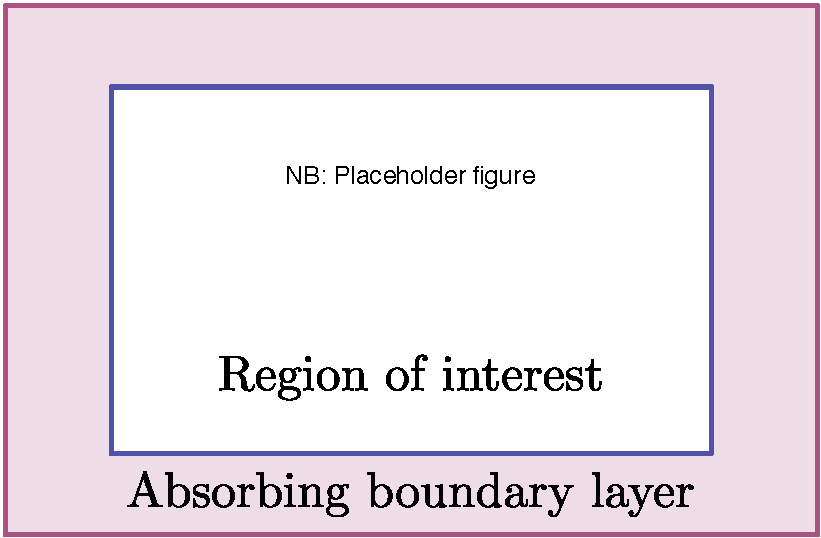
\includegraphics[width=8cm]{RegionOfInterest}
    \caption{A snapshot of the total density from a GP simulation corresponding to the system under discussion in this chapter. It can be observed that the atom laser density is decaying within the absorbing boundary layer. The region of interest and absorbing boundary layer are marked. The region of interest is the entire computational domain except for the absorbing boundary layer. The absorbing boundary layer has a width of $\unit[5]{\micro m}$. \label{Peaks:RegionOfInterest}}
\end{figure}

The rate and distribution with which momentum leaves the region of interest can be determined by considering the equation of motion for the wavenumber density in the region of interest,
\begin{align}
    \frac{\partial }{\partial t}\abs{\widetilde{\psi}_\text{roi}(\bm{k}, t)}^2 &= 2 \Re \left\{ \widetilde{\psi}_\text{roi}^*(\bm{k}, t) \frac{\partial }{\partial t}\widetilde{\psi}_\text{roi}(\bm{k}, t) \right \},
\end{align}
where $\widetilde{\psi}_\text{roi}(\bm{k}, t)$ is the Fourier transform of the restricted wavefunction $\psi_\text{roi}(\bm{x}, t)$, which is defined to be nonzero only within the region of interest. The equation of motion for $\widetilde{\psi}_\text{roi}(\bm{k}, t)$ is
\begin{align}
    \label{Peaks:PsikROIEquationOfMotion}
    \frac{\partial}{\partial t} \widetilde{\psi}_\text{roi}(\bm{k}, t) &= -\frac{i}{\hbar} \mathcal{F}\left[\left(-\frac{\hbar^2 \nabla^2}{2M} + V(\bm{x}) + U \abs{\psi_\text{roi}(\bm{x}, t)}^2\right) \psi_\text{roi}(\bm{x}, t)\right](\bm{k}),
\end{align}
where $\mathcal{F}[f(\bm{x})](\bm{k})$ denotes the Fourier transform of the function $f(\bm{x})$. While the potential and interaction terms in \eqref{Peaks:PsikROIEquationOfMotion} redistribute momentum, it is only due to the kinetic term that momentum will leave the region of interest. To see that this is true, consider a Hamiltonian with no kinetic term. In this case the local phase of the wavefunction will rotate, but the density distribution will remain unchanged. Hence it will be the kinetic term in \eqref{Peaks:PsikROIEquationOfMotion} that will determine the momentum density flux leaving the region of interest.

The Fourier transform of the kinetic term in \eqref{Peaks:PsikROIEquationOfMotion} can be evaluated to give the momentum density flux $\Phi(\bm{k}, t)$ leaving the region of interest in terms of a surface integral over the boundary of the region of interest,
\begin{align}
    \Phi(\bm{k}, t) & = -\frac{\partial }{\partial t}\abs{\widetilde{\psi}_\text{roi}(\bm{k}, t)}^2\bigg|_\text{kinetic}\\
    & = -2 \Re \left\{ \frac{i \hbar}{2 M} \widetilde{\psi}_\text{roi}^*(\bm{k}, t) \frac{1}{(2 \pi)^{\frac{3}{2}}}\oiint e^{-i \bm{k}\cdot \bm{x}} \Big[ \nabla \psi_\text{roi}(\bm{x}, t) + i \bm{k} \psi_\text{roi}(\bm{x}, t)\Big] \cdot d \bm{A} \right\}.
    \label{Peaks:MomentumDensityFluxSurfaceIntegral}
\end{align}
The $\psi_\text{roi}(\bm{x}, t)$ and $\nabla\psi_\text{roi}(\bm{x}, t)$ terms to be evaluated at the boundary in \eqref{Peaks:MomentumDensityFluxSurfaceIntegral} should be understood to be defined by the limit from the interior of the region of interest. While \eqref{Peaks:MomentumDensityFluxSurfaceIntegral} is the most direct way of evaluating $\Phi(\bm{k}, t)$, it is a computationally inefficient method as it requires the calculation of a surface integral for every point $\bm{k}$ at which we wish to evaluate $\Phi(\bm{k}, t)$. 

A more efficient method can be found by instead considering the evolution of the wavenumber density on the entire computational domain. The momentum flux density that left the region of interest enters the absorbing boundary layer through a term like \eqref{Peaks:MomentumDensityFluxSurfaceIntegral}, but leaves at a slightly later time due to the negative imaginary potential. As it is not the temporal dynamics of $\Phi(\bm{k}, t)$ in which we are interested, but just the distribution of momentum that left the region of interest at \emph{any} time, this delay is unimportant. On the entire computational domain, the two kinetic transport terms will cancel leaving the term due to the negative imaginary potential. Assuming that the mean-field interaction energy of the wavefunction reaching the absorbing boundary layer is small compared to its kinetic energy, the momentum flux density leaving the computational domain is given by
\begin{align}
    \label{Peaks:MomentumDensityFlux}
    \Phi(\bm{k}, t)&=\frac{2}{\hbar} \Re \left\{ \widetilde{\psi}^*(\bm{k}, t) \mathcal{F}'\left[ V_I(\bm{x}) \psi(\bm{x}, t)\right](\bm{k}) \right\},
\end{align}
where $\mathcal{F}'$ is the appropriate Fourier-like transform that connects the spatial and spectral representations of the wavefunction $\psi$, and guarantees the artificial boundary conditions are satisfied. Equation \eqref{Peaks:MomentumDensityFlux} is a more efficient method of evaluating $\Phi(\bm{k}, t)$ than \eqref{Peaks:MomentumDensityFluxSurfaceIntegral} as it only requires two Fourier-like transforms to evaluate $\Phi(\bm{k}, t)$ for all $\bm{k}$, instead of one surface integral \emph{for each} $\bm{k}$.

The information provided by either \eqref{Peaks:MomentumDensityFluxSurfaceIntegral} or \eqref{Peaks:MomentumDensityFlux} will only be as good as the absorbing boundary layer. While for a perfect absorbing boundary layer $\int \Phi(\bm{k}, t)\, dt$ would exactly equal the lost momentum density from the region of interest, for an imperfect absorbing boundary layer $\int \Phi(\bm{k}, t)\, dt$ will also include contributions due to any reflection from or transmission through the boundary layer. 

An example calculation of $\Phi(\bm{k}, t)$ for a finite absorbing boundary layer is given in \sectionref{MethodsAppendix:MomentumDensityFluxExampleCalculation}. There it is demonstrated that $\Phi(\bm{k}, t)$ is an accurate method for determining the rate of loss of momentum density from a region of space for the same range of momenta for which the absorbing boundary layer is itself accurate.

\parasep

The simulations described in the remainder of this chapter use the method presented in this section to determine the momentum distribution of atoms that have the left computational domain. This momentum distribution is then propagated classically under gravity to find the corresponding density distribution on the MCP detector below the condensate. This classical propagation was performed by \emph{Mattias Johnsson}. Note that due to the use of cylindrical symmetry, the correct Fourier-like transform for use in \eqref{Peaks:MomentumDensityFlux} is the Hankel (or Bessel) transform \citep{ArfkenWeber}.

\subsection{Equations of motion}
\label{Peaks:3DEquationsOfMotion}

Having described the calculational techniques that will be used, we now turn to the description of the Gross-Pitaevskii and Truncated Wigner equations that were used to model the experiment. The GP equations that correspond to the master equation \eqref{Peaks:MasterEquation} are
\begin{subequations}
    \label{Peaks:3DGPEquations}
    \begin{align}
        \begin{split}
            i \hbar \frac{\partial }{\partial t}\Psi_1 &= \frac{-\hbar^2 \nabla^2}{2 M} \Psi_1 + \big(V_\text{trap}(\bm{x}) - i V_I(\bm{x})\big)\Psi_1 + \sqrt{2} \hbar \Omega \Psi_0 \\
            & \relphantom{=} + c_0 \sum_j \abs{\Psi_j}^2 \Psi_1 + c_2\left(\abs{\Psi_1}^2 + \abs{\Psi_0}^2 - \abs{\Psi_{-1}}^2 \right) \Psi_1 + c_2 \Psi_{-1}^*\Psi_0^2 \\
            & \relphantom{=} - i \hbar\frac{3}{2}K^\text{(unpol)}_{^{4}\text{He}} \left(2\abs{\Psi_{-1}}^2 \Psi_1 - \Psi_{-1}^* \Psi_0^2\right),
        \end{split}\\
        \begin{split}
            i \hbar \frac{\partial }{\partial t}\Psi_0 &= \frac{-\hbar^2 \nabla^2}{2 M} \Psi_0 + \big(\hbar \Delta - i V_I(\bm{x}) \big)\Psi_0 + \sqrt{2} \hbar \Omega \Psi_1 + \sqrt{2}\hbar\Omega \Psi_{-1} \\
            & \relphantom{=} + c_0 \sum_j \abs{\Psi_j}^2 \Psi_0 + c_2\left(\abs{\Psi_1}^2 + \abs{\Psi_{-1}}^2 \right) \Psi_0 + 2 c_2 \Psi_{0}^*\Psi_1\Psi_{-1} \\
            & \relphantom{=} - i \hbar\frac{3}{2}K^\text{(unpol)}_{^{4}\text{He}} \left(\abs{\Psi_{0}}^2 \Psi_0 - 2\Psi_{0}^* \Psi_1\Psi_{-1}\right),
        \end{split}\\
        \begin{split}
            i \hbar \frac{\partial }{\partial t}\Psi_{-1} &= \frac{-\hbar^2 \nabla^2}{2 M} \Psi_{-1} + \big(-V_\text{trap}(\bm{x}) + 2 \hbar \Delta - i V_I(\bm{x})\big)\Psi_{-1} + \sqrt{2} \hbar \Omega \Psi_0 \\
            & \relphantom{=} + c_0 \sum_j \abs{\Psi_j}^2 \Psi_{-1} + c_2\left(-\abs{\Psi_1}^2 + \abs{\Psi_0}^2 + \abs{\Psi_{-1}}^2 \right) \Psi_{-1} + c_2 \Psi_{1}^*\Psi_0^2 \\
            & \relphantom{=} - i \hbar\frac{3}{2}K^\text{(unpol)}_{^{4}\text{He}} \left(2\abs{\Psi_{1}}^2 \Psi_{-1} - \Psi_{1}^* \Psi_0^2\right),
        \end{split}
    \end{align}
\end{subequations}
where $\displaystyle V_\text{trap}(\bm{x}) = \frac{1}{2} M \left(\omega_r^2 r^2 + \omega_z^2 z^2 \right)$ is the trapping potential, $\hbar \Delta$ is the detuning in energy of the resonant outcoupling surface from the centre of the condensate, $c_0 = (g_0 + 2 g_2)/3$, $c_2 = (g_2 - g_0)/3$, where $g_S = 4 \pi \hbar^2 a_S/M$ is the nonlinear interaction strength, and $a_S$ is the $s$-wave scattering length for the total hyperfine spin $S$ channel (refer to \sectionref{BackgroundTheory:Helium}). A derivation of the Penning ionisation terms in \eqref{Peaks:3DGPEquations} is given in \sectionref{PenningIonisationAppendix:GP}.

The Truncated Wigner equations corresponding to the master equation \eqref{Peaks:MasterEquation} are very similar to \eqref{Peaks:3DGPEquations} but with some additional terms. In Stratonovich form, the equations of motion for the stochastic wavefunctions are approximately
% See MolecularScattering.nb for the derivation of the Penning ionisation terms
\begin{align}
    \label{Peaks:3DTWEquations}
    \begin{split}
        \left. i \hbar \,d\bm{\Psi}\right|_\text{TW} &\approx \left. i \hbar \frac{\partial }{\partial t}\bm{\Psi}\right|_\text{GP} dt - \left(2 c_0 + c_2 \right)\frac{1}{\Delta V}\bm{\Psi}\, dt\\
        &\relphantom{\approx} + i\sqrt{ \hbar V_I(\bm{x})} \,d\bm{W}(\bm{x}) + i \hbar\sqrt{3 \Kunpol}
        \begin{pmatrix}
            \Psi_{-1}^*\\
            \Psi_0^*\\
            \Psi_1^*
        \end{pmatrix} dW_p(\bm{x}),
    \end{split}
\end{align}
where $\Delta V$ is the computational grid's volume element (for irregularly spaced grids such as those that used for cylindrically symmetric problems, $\Delta V$ is the local Gaussian quadrature weight \citep{Ronen:2006}), $\bm{\Psi} = \left(\Psi_1, \Psi_0, \Psi_{-1} \right)^T$ and $d \bm{W}(\bm{x}) = \big(dW_1(\bm{x}), dW_0(\bm{x}), dW_{-1}(\bm{x})\big)^T$ and $dW_p(\bm{x})$ are the complex Gaussian noises satisfying
\begin{align}
    \overline{dW_i(\bm{x})\, dW_j(\bm{x}')} &= 0 \\
    \overline{dW_i(\bm{x})\, dW_j^*(\bm{x}')} &= \frac{1}{\Delta V}\delta_{ij}\delta_{\bm{x},\bm{x}'}\,dt, \label{Peaks:ComplexNoiseExpectationValue}
\end{align}
where $\overline{(\cdot)}$ denotes the expectation value taken with respect to the noises. The usual spatial Dirac delta function in \eqref{Peaks:ComplexNoiseExpectationValue} has been replaced by a Kronecker delta function scaled by the inverse volume element due to the discretisation of the problem onto a computational grid.

The origin of the additional terms in \eqref{Peaks:3DTWEquations} can be understood qualitatively in terms of the `virtual' particles added to the initial state required in Truncated Wigner (see \sectionref{BackgroundTheory:TruncatedWigner}). The $\Delta V^{-1}$ term corrects for the contribution to \emph{s}-wave scattering due to the virtual particles. The $d \bm{W}$ term corrects for the loss of virtual particles due to the absorbing boundary layer and the $dW_p$ term does similarly for the virtual particles lost due to Penning ionisation.

The approximation made in obtaining \eqref{Peaks:3DTWEquations} was to neglect $\Delta V^{-1}$ compared to the field occupations $\abs{\Psi_1}^2$, $\abs{\Psi_0}^2$, $\abs{\Psi_{-1}}^2$ in the Penning ionisation noise term. This is justified for large occupations where Penning ionisation will be significant. The approximation cannot be made where the density is low, but at these locations the Penning ionisation process itself can be neglected as the associated rate constant will have decreased proportionally with the density. A derivation of the Penning ionisation noise term in \eqref{Peaks:3DTWEquations} is given in \sectionref{PenningIonisationAppendix:TW}.

\parasep

One might like to imagine that the task is essentially complete once a set of equations has been derived that describes a system. Unfortunately, technical considerations often limit which problems are and are not feasible to solve. In this case, although the GP equations given in \eqref{Peaks:3DGPEquations} can be solved in a couple of days on a supercomputer, \eqref{Peaks:3DTWEquations} represents a much more challenging problem. Not only do these equations need to be solved a large number of times for different initial conditions, but algorithms for solving stochastic differential equations are limited to a lower order\footnote{There is no known bound on the order of algorithms for solving stochastic (partial) differential equations, however algorithms for strong solutions require the evaluation of an exponentially increasing number of higher-order noise integrals with increasing order of the algorithm \citep{Burrage:1997}. For weak solutions (what is required here) the highest-order algorithms known that only require the evaluation of $O(N)$ noise integrals have global order $O(\Delta t^2)$ \citep{Rosler:2007,Rosler:2009}, where $N$ is the number of Gaussian noises required (as the noises are spatially-dependent, $N$ is proportional to the size of the computational grid and hence the evaluation of $O(N^2)$ or more noise integrals is infeasible).} than those that can be used for deterministic differential equations hence significantly smaller time steps are required for solving stochastic differential equations. This problem is mainly due to the $\Psi_{-1}$ state which, due to the antitrapping potential, has a kinetic energy $\sim 40$ times larger than the $\Psi_{0}$ atoms at the edge of the computational domain $\unit[60]{\micro m}$ away from the centre of the condensate in the radial direction. The computational domain cannot be restricted to be tighter due to the requirement that the mean-field energy of the $\Psi_{0}$ atoms be negligible compared to their kinetic energy for the absorbing boundary layer to be effective. While it is for these practical reasons that we must neglect the $\Psi_{-1}$ state, we are physically justified in doing so by the same arguments given at the start of \sectionref{Peaks:PerturbativeApproach}. 

In the next sections the behaviour of the atom laser in the cases of outcoupling from the centre of the condensate (resonant outcoupling) and outcoupling from a detuned surface where the atom laser flux is maximised are considered.

\subsection{Verification of semianalytical model}

As a verification of the results of \sectionref{Peaks:PerturbativeApproach} we consider outcoupling from the centre of the condensate ($\Delta = 0$). This is the case that corresponds most closely with that of the homogenous condensate considered in \sectionref{Peaks:PerturbativeApproach} because the shape of the outcoupling surfaces (see \figureref{Peaks:OutcouplingSurfaces}) restricts outcoupling to the centre of the condensate where the density is a local maximum; there the condensate is locally homogeneous.

\begin{figure}
    \centering
    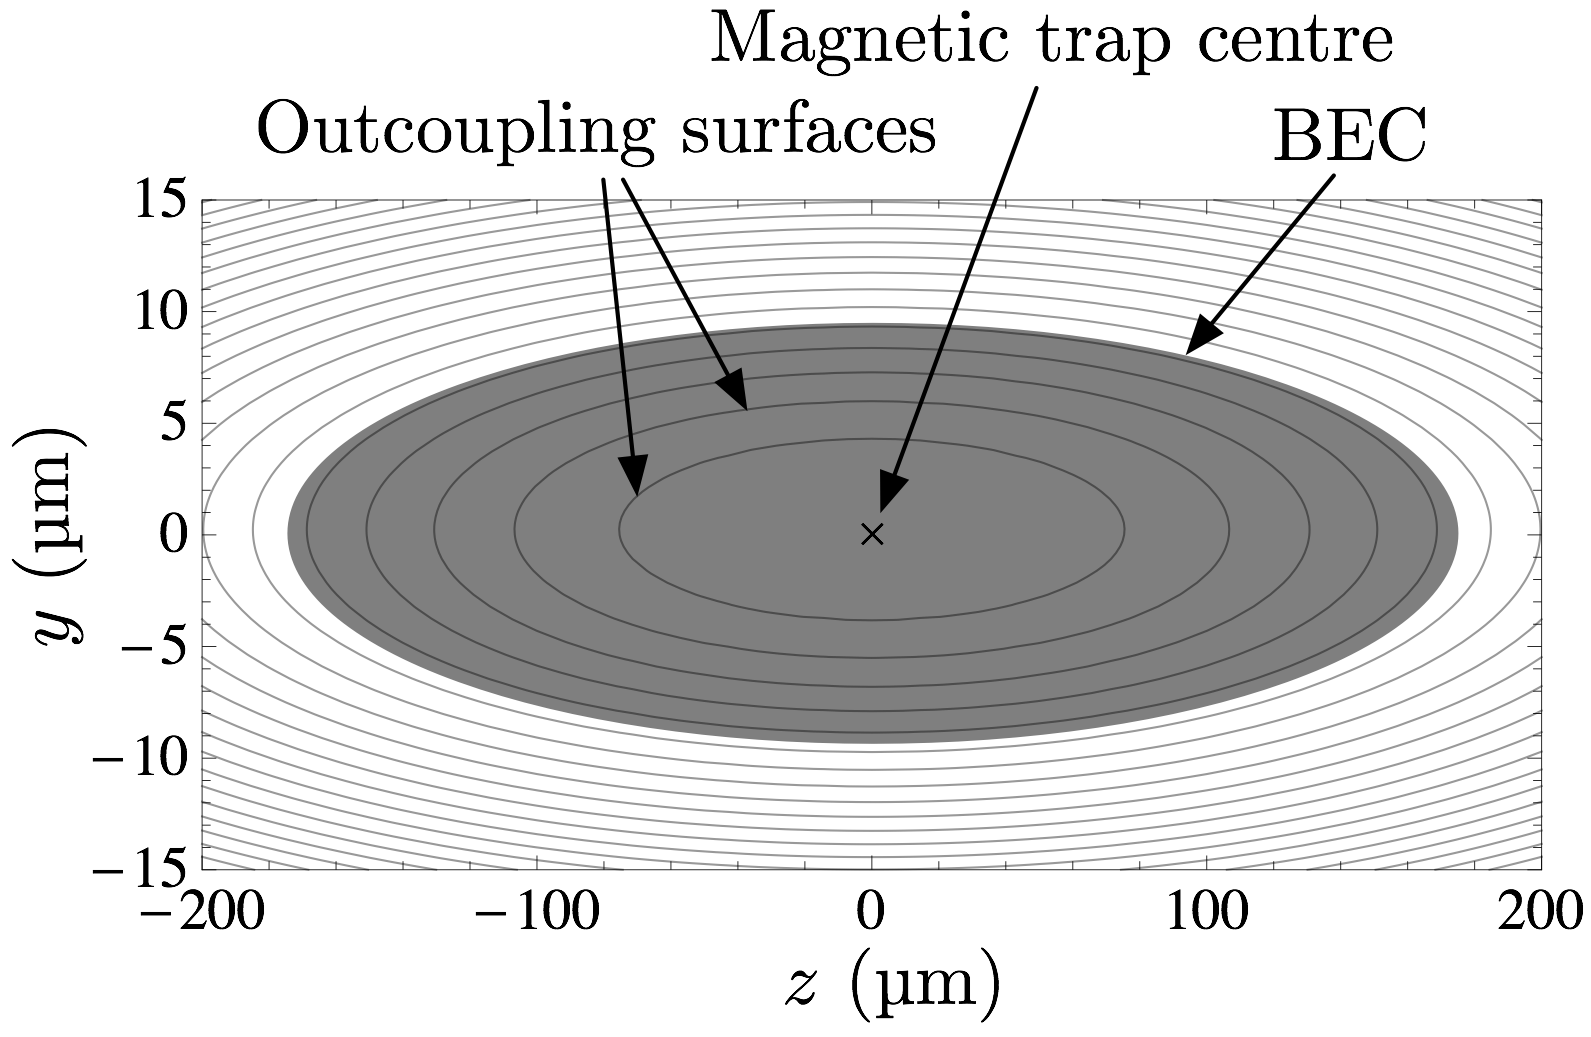
\includegraphics[width=8cm]{OutcouplingSurfaces}
    \caption{Outcoupling surfaces of the He* condensate under consideration in this chapter. The small gravitational sag of $y_\text{sag} = \unit[0.2]{\micro m}$ means that the centre of the trap and the centre of the condensate almost exactly coincide. Hence the outcoupling surfaces are approximately centred on the centre of the condensate. The contours pictured are equally-spaced in energy. Note that the aspect ratio of this figure is not 1:1 for reasons of clarity; the condensate is significantly more elongated than as pictured. \label{Peaks:OutcouplingSurfaces}}
\end{figure}

\begin{figure}
    \centering
    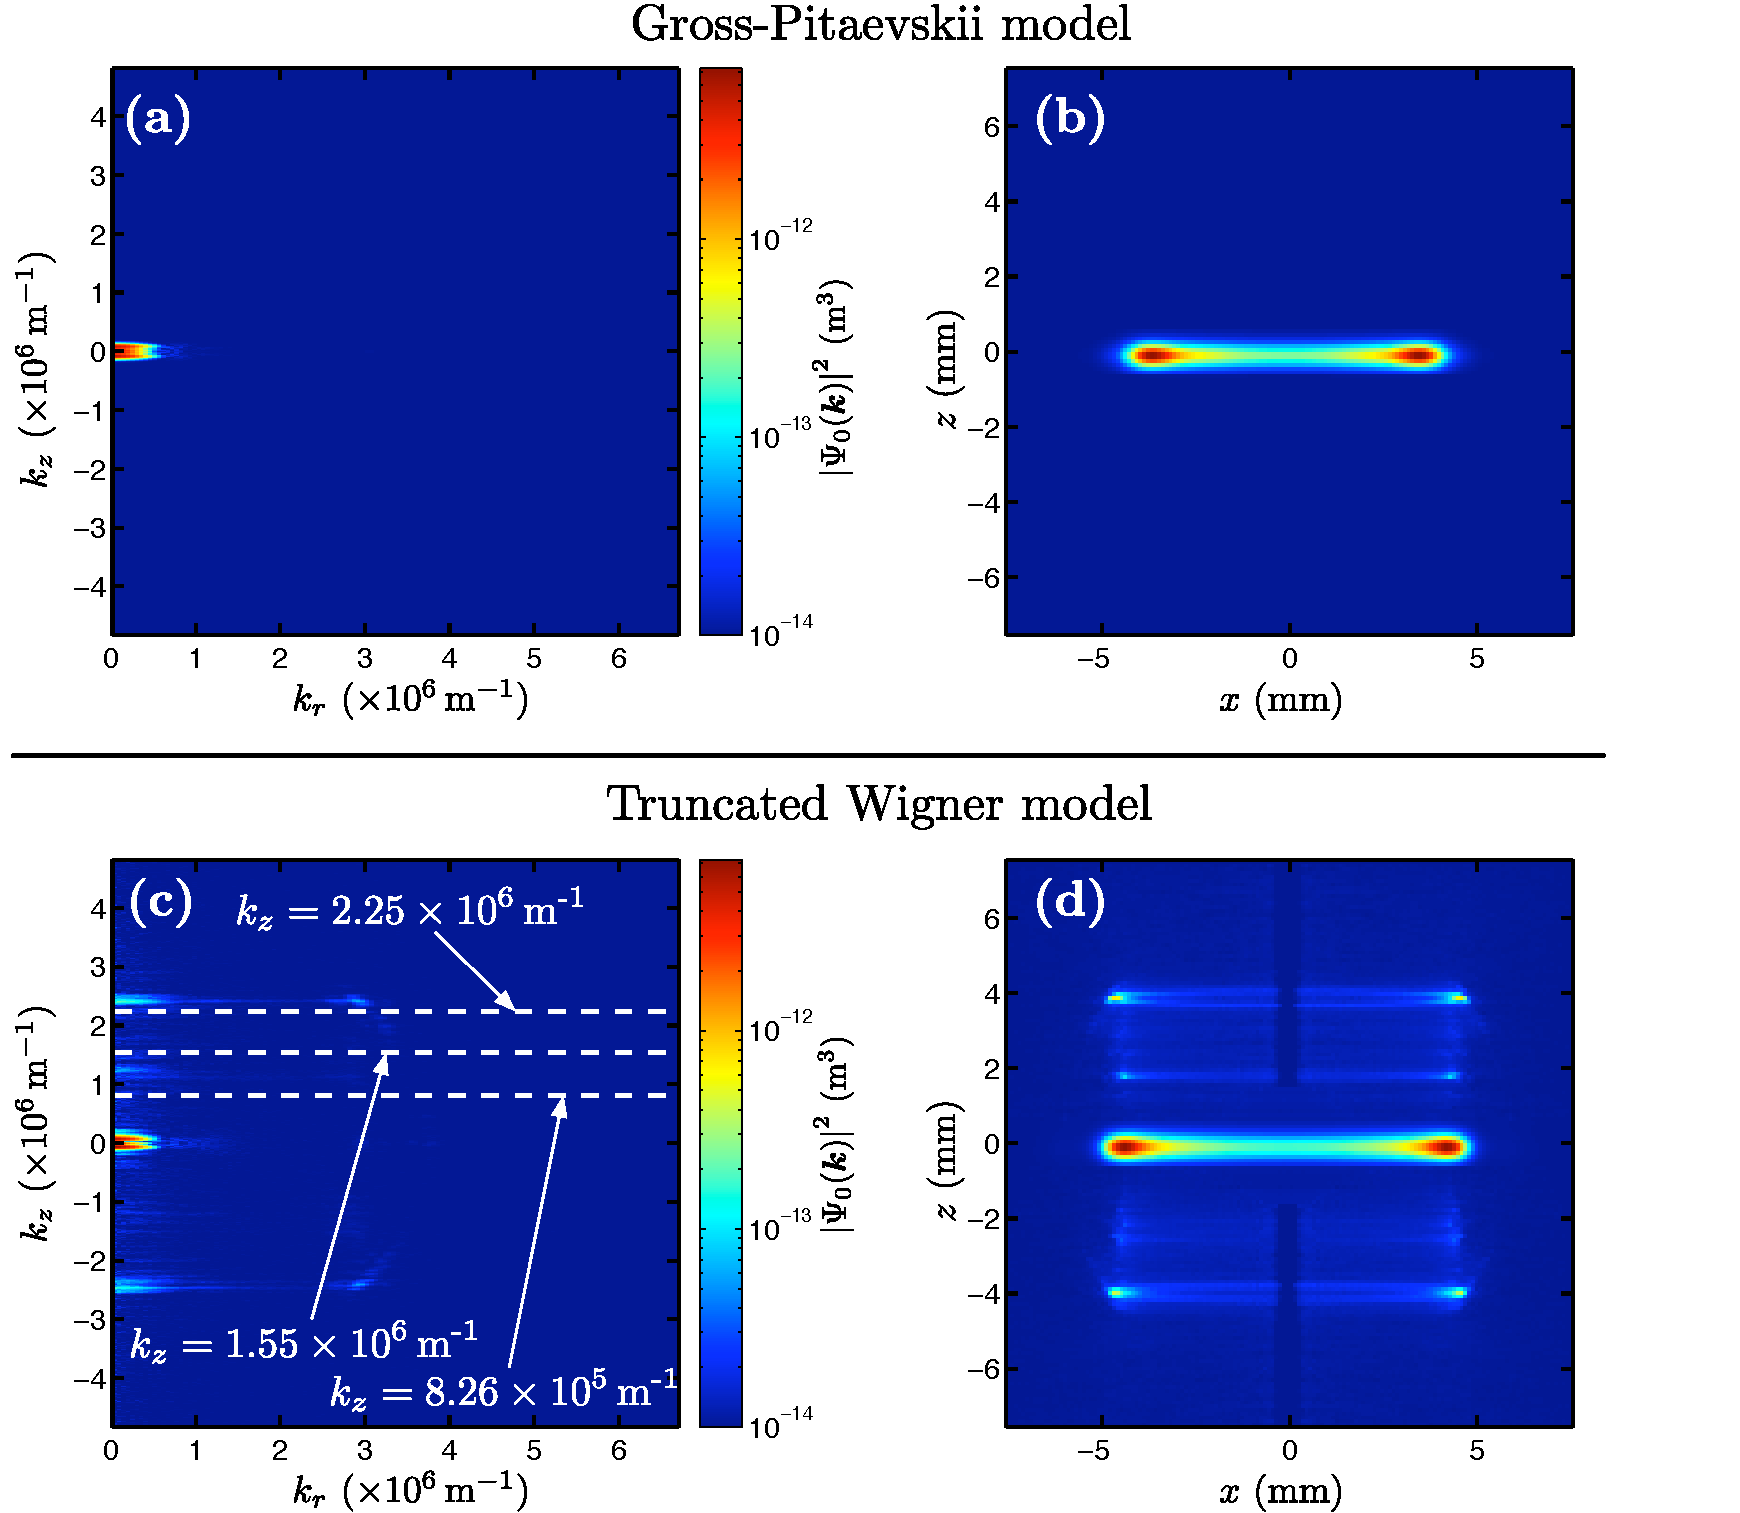
\includegraphics[trim=0 0 52 0,width=14cm]{ResonantOutcouplingNoPI}
    \caption{Simulation results for outcoupling from the centre of the condensate without Penning ionisation. Left figures (a) and (c) plot the momentum density of the untrapped state at $t=\unit[2]{ms}$ as a function of the radial ($k_r$) and axial ($k_z$) wavenumbers. Right figures (b) and (d) plot the normalised density profiles that would be observed on the MCP detector $\unit[4]{cm}$ below the condensate due to outcoupling from the condensate for $t=\unit[6]{ms}$. The upper figures (a) and (b) plot the results of a GP model where the $m_F=-1$ state is assumed negligible, lower figures (e) and (f) correspond to a Truncated Wigner simulation for the same system averaged over $N_\text{realisations} = 4$. The wavenumbers of the three fastest-growing instabilities predicted by the perturbation analysis performed in \sectionref{Peaks:PerturbativeApproach} are marked in (c). The weak axis is in the vertical direction in all figures.\label{Peaks:TheoryZeroDetuningNoPIResults}}
\end{figure}

The results of the GP and TW simulations for the case of resonant outcoupling but in the absence of Penning ionisation are presented in \figureref{Peaks:TheoryZeroDetuningNoPIResults}. The atom laser momentum density for the GP and TW simulations are displayed in \figureref{Peaks:TheoryZeroDetuningNoPIResults}(a) and (c). The primary contribution to the momentum density is around $(k_r \approx 0, k_z \approx 0)$ due to Rabi coupling to the Bose-Einstein condensate. Due to the high aspect ratio of the condensate, these atoms are strongly accelerated along the radial direction and hence move to the right in \figureref{Peaks:TheoryZeroDetuningNoPIResults}(a) and (c). At times earlier than $t=\unit[2]{ms}$ which is pictured in \figureref{Peaks:TheoryZeroDetuningNoPIResults}(a) and (c) there is an additional peak at $(k_r \approx \unit[2.8 \times 10^6]{m}^{-1}, k_z \approx 0)$ due to the main atom laser after it has accelerated out of the condensate. This peak disappears around $t=\unit[1.8]{ms}$ due to the formation of a bound state (see \citep{Robins:2005uq}\footnote{FIXME: If JD gets his paper published, that needs citing here.}) causing the atom laser to shutdown.

The primary feature of the MCP detector profiles depicted in \figureref{Peaks:TheoryZeroDetuningNoPIResults}(b) and (d) is the atom laser profile in the middle of both images. The double-peak structure of the atom laser profile was discussed earlier in \sectionref{TransverseProfile:Helium}. Briefly, the broad structure is due to the strong acceleration of the atom laser out of the condensate in the radial direction leading to a ring in momentum space (the peak at $(k_r \approx \unit[2.8 \times10^6]{m}^{-1}, k_z \approx 0)$ discussed above). Due to the expansion of the atom laser during as it falls, the measured density on the MCP detector corresponds to the vertically integrated momentum distribution as depicted in \figureref{Peaks:Schematic}. The vertical integration of the ring-shaped momentum distribution directly leads to the double-peak structure in the main atom laser profile in \figureref{Peaks:TheoryZeroDetuningNoPIResults}(b) and (d). Neither the fine structure nor the `shadow' of the BEC in the atom laser profile discussed in \sectionref{TransverseProfile:Helium} are observed in \figureref{Peaks:TheoryZeroDetuningNoPIResults} due to the use of a purely classical method to propagate the momentum density from the edge of the computational region to the detector. However these details are not of interest in this chapter.

The spontaneously-seeded dynamical instabilities predicted in \sectionref{Peaks:PerturbativeApproach} are observed in the results of the Truncated Wigner model shown in \figureref{Peaks:TheoryZeroDetuningNoPIResults}, but absent from the results of the Gross-Pitaevskii model due to its neglect of spontaneously-seeded processes. Moreover, the dynamical instability with the largest growth rate illustrated in \figureref{Peaks:CondensateEigenvalues} at $k=\unit[2.25\times 10^6]{m}^{-1}$ is in good agreement with the highest growth rate instability in \figureref{Peaks:TheoryZeroDetuningNoPIResults}(c) observed at $(k_r \approx 0,\, k_z \approx \pm\unit[2.4\times 10^6]{m}^{-1})$. As discussed above this instability is outcoupled from the condensate and then accelerates radially outwards (to the right in \figureref{Peaks:TheoryZeroDetuningNoPIResults}(c)) to produce rings in momentum space. These rings appear as the double-peaked structures on the MCP detector away from the main atom laser profile in \figureref{Peaks:TheoryZeroDetuningNoPIResults}(d). The formation process of the instabilities is illustrated in \figureref{Peaks:ResonantOutcouplingProcess} and a comparison is made to the results of the GP model in which these instabilities do not occur\footnote{Although not pictured, the instabilities \emph{are} observed in the GP model, appearing just after $t=\unit[6]{ms}$. The appearance of these instabilities however is not for physical reasons, instead it is caused by the amplification of numerical noise in the simulation. A higher-precision GP simulation would show the instabilities appearing at a later time.}.

\begin{sidewaysfigure}
    \centering
    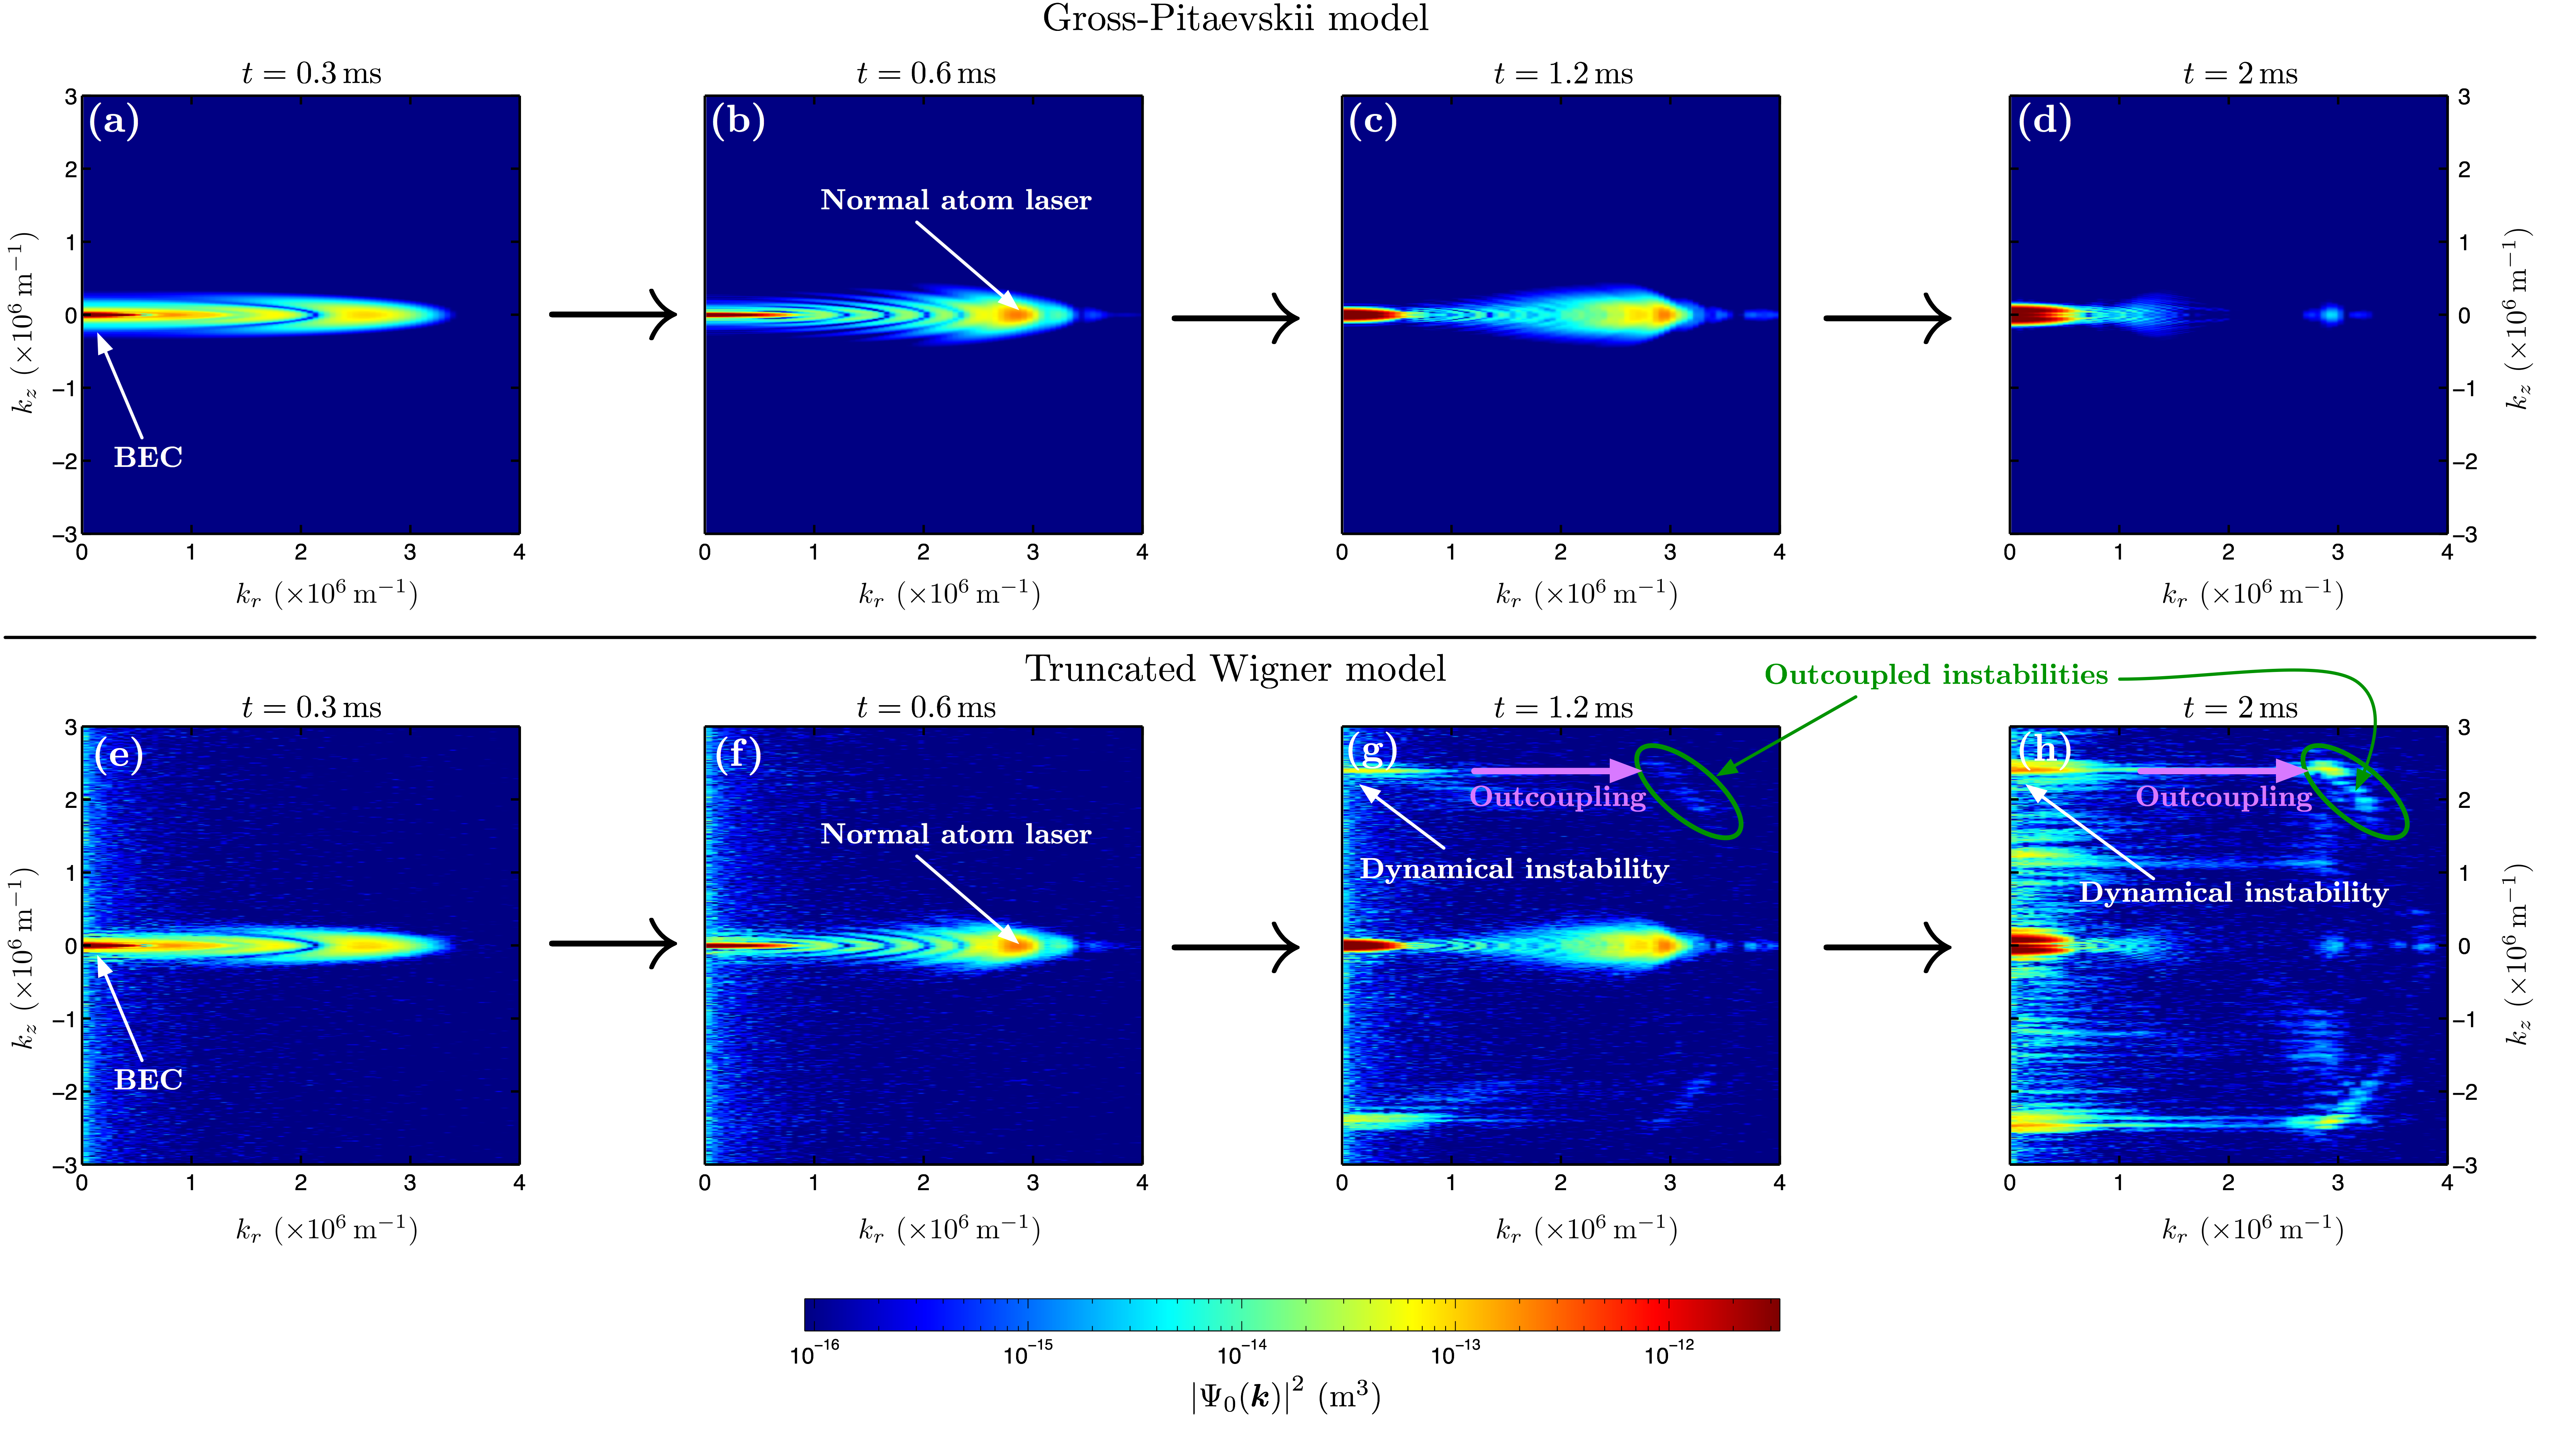
\includegraphics[width=22cm]{ResonantOutcouplingProcess}
    \caption{Simulation results for outcoupling from the centre of the condensate without Penning ionisation illustrating the formation of the normal atom laser profile and the dynamical instabilities. Upper figures (a)--(d) are the results of a two level Gross-Pitaevskii model, and lower figures (e)--(h) are the results of a two level Truncated Wigner model. The upper and lower rows respectively correspond to the upper and lower rows of \figureref{Peaks:TheoryZeroDetuningNoPIResults}. The columns from left to right show the evolution of the momentum density $\abs{\Psi_0(\bm{k})}^2$ of the untrapped state at times: \unit[0.3]{ms}, \unit[0.6]{ms}, \unit[1.2]{ms}, and \unit[2]{ms}.
    This figure illustrates that the instabilities are spontaneously seeded and that modes between the main atom laser profile and the instabilities are not significantly populated until after the instability has formed. The marked `Normal atom laser' part of the momentum density distribution is the component that corresponds to the MCP atom laser profile shown in \figureref{Peaks:TheoryZeroDetuningNoPIResults}(b).  Note that the vacuum noise in (e)--(h) is not uniform because the initial vacuum noise is proportional to the inverse volume element, which due to the assumed cylindrical symmetry $\displaystyle \Delta V_{\bm{k}}^{-1} \propto k_r^{-1}$.\label{Peaks:ResonantOutcouplingProcess}}
\end{sidewaysfigure}

As discussed in \sectionref{Peaks:DynamicalInstabilitiesDiscussion} the dynamical instabilities observed in \figureref{Peaks:TheoryZeroDetuningNoPIResults} will be entangled when they are produced, however the entangled modes are superpositions of the $\Psi_1$ and $\Psi_0$ states with opposite momenta. It will not be feasible to directly detect this entanglement as the outcoupling process will significantly complicate the spatial structure of the entangled modes. Although only the $\Psi_0$ state can leave the magnetic trap, the $\Psi_1$ component of the entangled mode is likely to be outcoupled faster than the time it would take to perform half an oscillation and reverse the sign of its axial momentum ($\sim \unit[9]{ms}$). Consequently number difference squeezing between the opposite momentum components of the entangled modes should be robust enough to survive outcoupling. It cannot be proven due to the small number of realisations calculated, however it is expected that there should exist number difference squeezing between the number of atoms above and below the main atom laser beam in \figureref{Peaks:TheoryZeroDetuningNoPIResults}. The main atom laser beam must be excluded as it is produced due to entirely classical means and hence would not be have number difference squeezing.

Although not pictured, the results of a GP model including all three atomic levels $\Psi_1$, $\Psi_0$ and $\Psi_{-1}$ are of the same form as the results presented in \figureref{Peaks:TheoryZeroDetuningNoPIResults}(a) and (b).




% \subsubsection{In the presence of Penning ionisation}
% Including Penning ionisation in the GP and TW simulations complicates the comparison of the results with the perturbative model presented in \sectionref{Peaks:PerturbativeApproach} as Penning ionisation will interfere with the growth processes and possibly suppress them. The results of GP and TW simulations for the case of resonant outcoupling and in the presence of Penning ionisation are presented in \figureref{Peaks:TheoryZeroDetuningPIResults}. It is noted that the spontaneously seeded structures observed in \figureref{Peaks:TheoryZeroDetuningNoPIResults} blah blah blah.
% 
% \begin{figure}
%     \centering
%     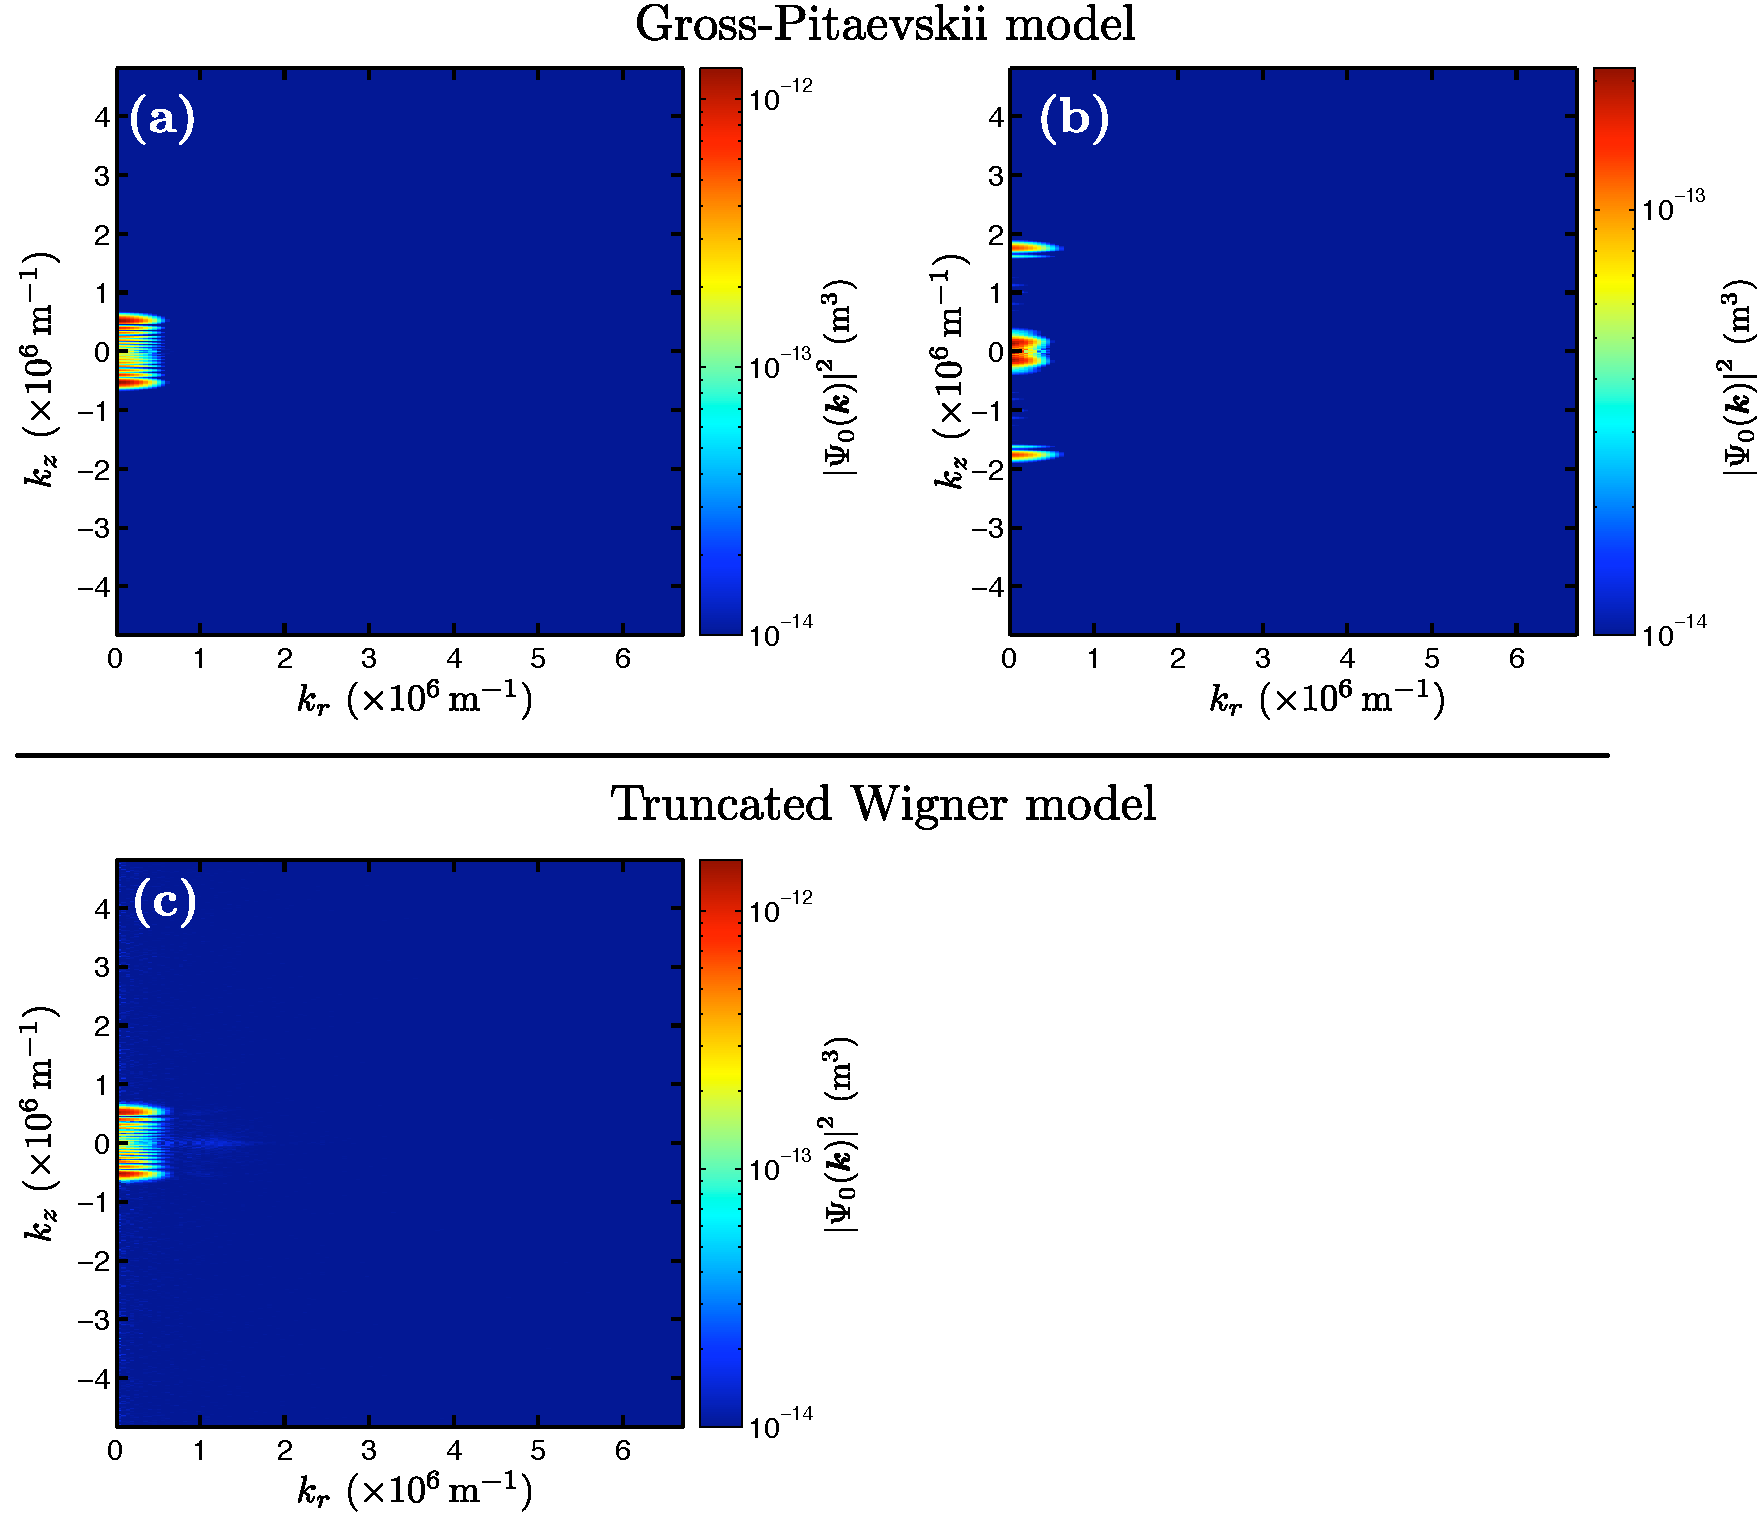
\includegraphics[width=14cm]{ResonantOutcouplingPI}
%     \caption{\label{Peaks:TheoryZeroDetuningPIResults} Simulation results for outcoupling from the centre of the condensate with Penning ionisation.}
% \end{figure}



% 
% The case in which Penning ionisation
% 
% \hrule
% 
% Next step: Penning ionisation.
% 
% As expected, the spontaneously-seeded dynamical instabilities predicted in \sectionref{Peaks:PerturbativeApproach} are not observed in the GP simulations where spontaneous scattering does not occur. Moreover, two of the dynamical instabilities predicted in \sectionref{Peaks:PerturbativeApproach} are observed in the results of the TW simulation with the third indistinguishable from the vacuum fluctuations due to the small number of realisations used. Although Penning ionisation was not considered in \sectionref{Peaks:PerturbativeApproach}, it can be seen from the results presented in \figureref{Peaks:TheoryZeroDetuningNoPIResults} that the instabilities have not been suppressed by Penning ionisation.
% 
% As the instabilities in \figureref{Peaks:TheoryZeroDetuningNoPIResults}(c) are outcoupled it can be observed that they accelerate along the radial direction forming momentum cones such as those pictured in \figureref{Peaks:Schematic}. When these momentum cones fall onto the detector they are vertically integrated to produce the well-defined peak-like structures in \figureref{Peaks:TheoryZeroDetuningNoPIResults}(d). Although these instabilities are entangled upon formation, it is unlikely that any useful entanglement will survive the outcoupling process as it is only the $\Psi_0$ and $\Psi_{-1}$ states that can escape the condensate. Despite this, it is likely that there will be number-difference squeezing between opposite points on the momentum cones as the characteristic time for the outcoupling process $\sim \unit[3]{ms}$ is much less than the time for an atom to undergo an oscillation in the weak trapping direction of $\sim \unit[18]{ms}$. Consequently, it is unlikely that the $\Psi_1$ component of the instability will remain in the condensate long enough for its momentum in the weak trapping dimension to change significantly. This number-difference squeezing between opposite points on the momentum-cones would be observed as a number difference squeezing between the structures on the opposite sides of the main atom laser profile in \figureref{Peaks:TheoryZeroDetuningNoPIResults}(d). Unfortunately, due to the computational difficulty of the problem, it is not at present possible to theoretically verify the claim of number-difference squeezing due to the large number of realisations that would be required for any results to have statistical significance.
% 
% To take into account the estimated expansion due to mean-field repulsion in the beam itself, we use an approximate method where we convolve the detector profiles with a Gaussian of width $\unit[200]{\micro m}$.
% 


\subsection{Comparison of Theory and Experiment}

In the previous section the behaviour of the atom laser when outcoupling from the centre of the condensate was considered.  In this limit it was found that the results of full 3D simulations were in good agreement with the semianalytical model presented in \sectionref{Peaks:PerturbativeApproach}.  The features in \figureref{Peaks:TheoryZeroDetuningNoPIResults}(d) and \figureref{Peaks:ExperimentalResults}(b) should therefore be interpreted as the result of the dynamical instabilities discussed in \sectionref{Peaks:PerturbativeApproach}. 

While the theoretical results presented in \figureref{Peaks:TheoryZeroDetuningNoPIResults}(d) show some similarity to the experimental results [\figureref{Peaks:ExperimentalResults}(b)], there are qualitative differences.  As will be shown in this section, these qualitative differences are due to the difference in detunings used in these two results.  While the theoretical results were for the case of outcoupling from the centre of the condensate, the experimental results were for the case of detuned outcoupling.  Resonant outcoupling can be understood in terms of the semianalytical model presented in \sectionref{Peaks:PerturbativeApproach} as the multimode behaviour of the full condensate only affects the dynamics weakly because the net force on atoms outcoupled from the centre of the trap is zero.  The direct application of the semianalytical model for detuned outcoupling is complicated by the multimode dynamics which are now evolve on a comparable timescale to the instabilities due to the nonzero net force on outcoupled atoms.  Although the model cannot be directly applied in this case it is reasonable to expect similar behaviour.  This expectation must be checked numerically.

The experimental results presented in \figureref{Peaks:ExperimentalResults} were not obtained by outcoupling from the centre of the condensate but instead a nonzero detuning of $\Delta = 2 \pi \times \unit[6.5]{kHz}$ was used, which is a significant fraction of the chemical potential $\mu/\hbar = 2\pi \times \unit[18]{kHz}$. This detuning was for the practical reason that when outcoupling near the centre of the condensate, the atom laser flux \emph{decreases} as the outcoupling surface moves towards the centre of the condensate (for the same rf outcoupling power). This behaviour can be explained using a simple model in which the  outcoupled atom laser flux is proportional to the surface area of the outcoupling surface times the average density over that surface. Outcoupling from the centre of the condensate will therefore lead to a small atom laser flux due to the small surface area (see \figureref{Peaks:OutcouplingSurfaces}). Detuning will cause the atom laser flux to increase as the surface area increases before decreasing again as the condensate density drops off towards the edge of the condensate. This behaviour is shown in \figureref{Peaks:DetuningCurve}. The experimental results presented in \figureref{Peaks:ExperimentalResults} were for the detuning which maximises the atom laser flux, which can be seen from \figureref{Peaks:DetuningCurve} to be $\Delta = 2\pi \times \unit[6.5]{kHz}$.

\begin{figure}
    \centering
    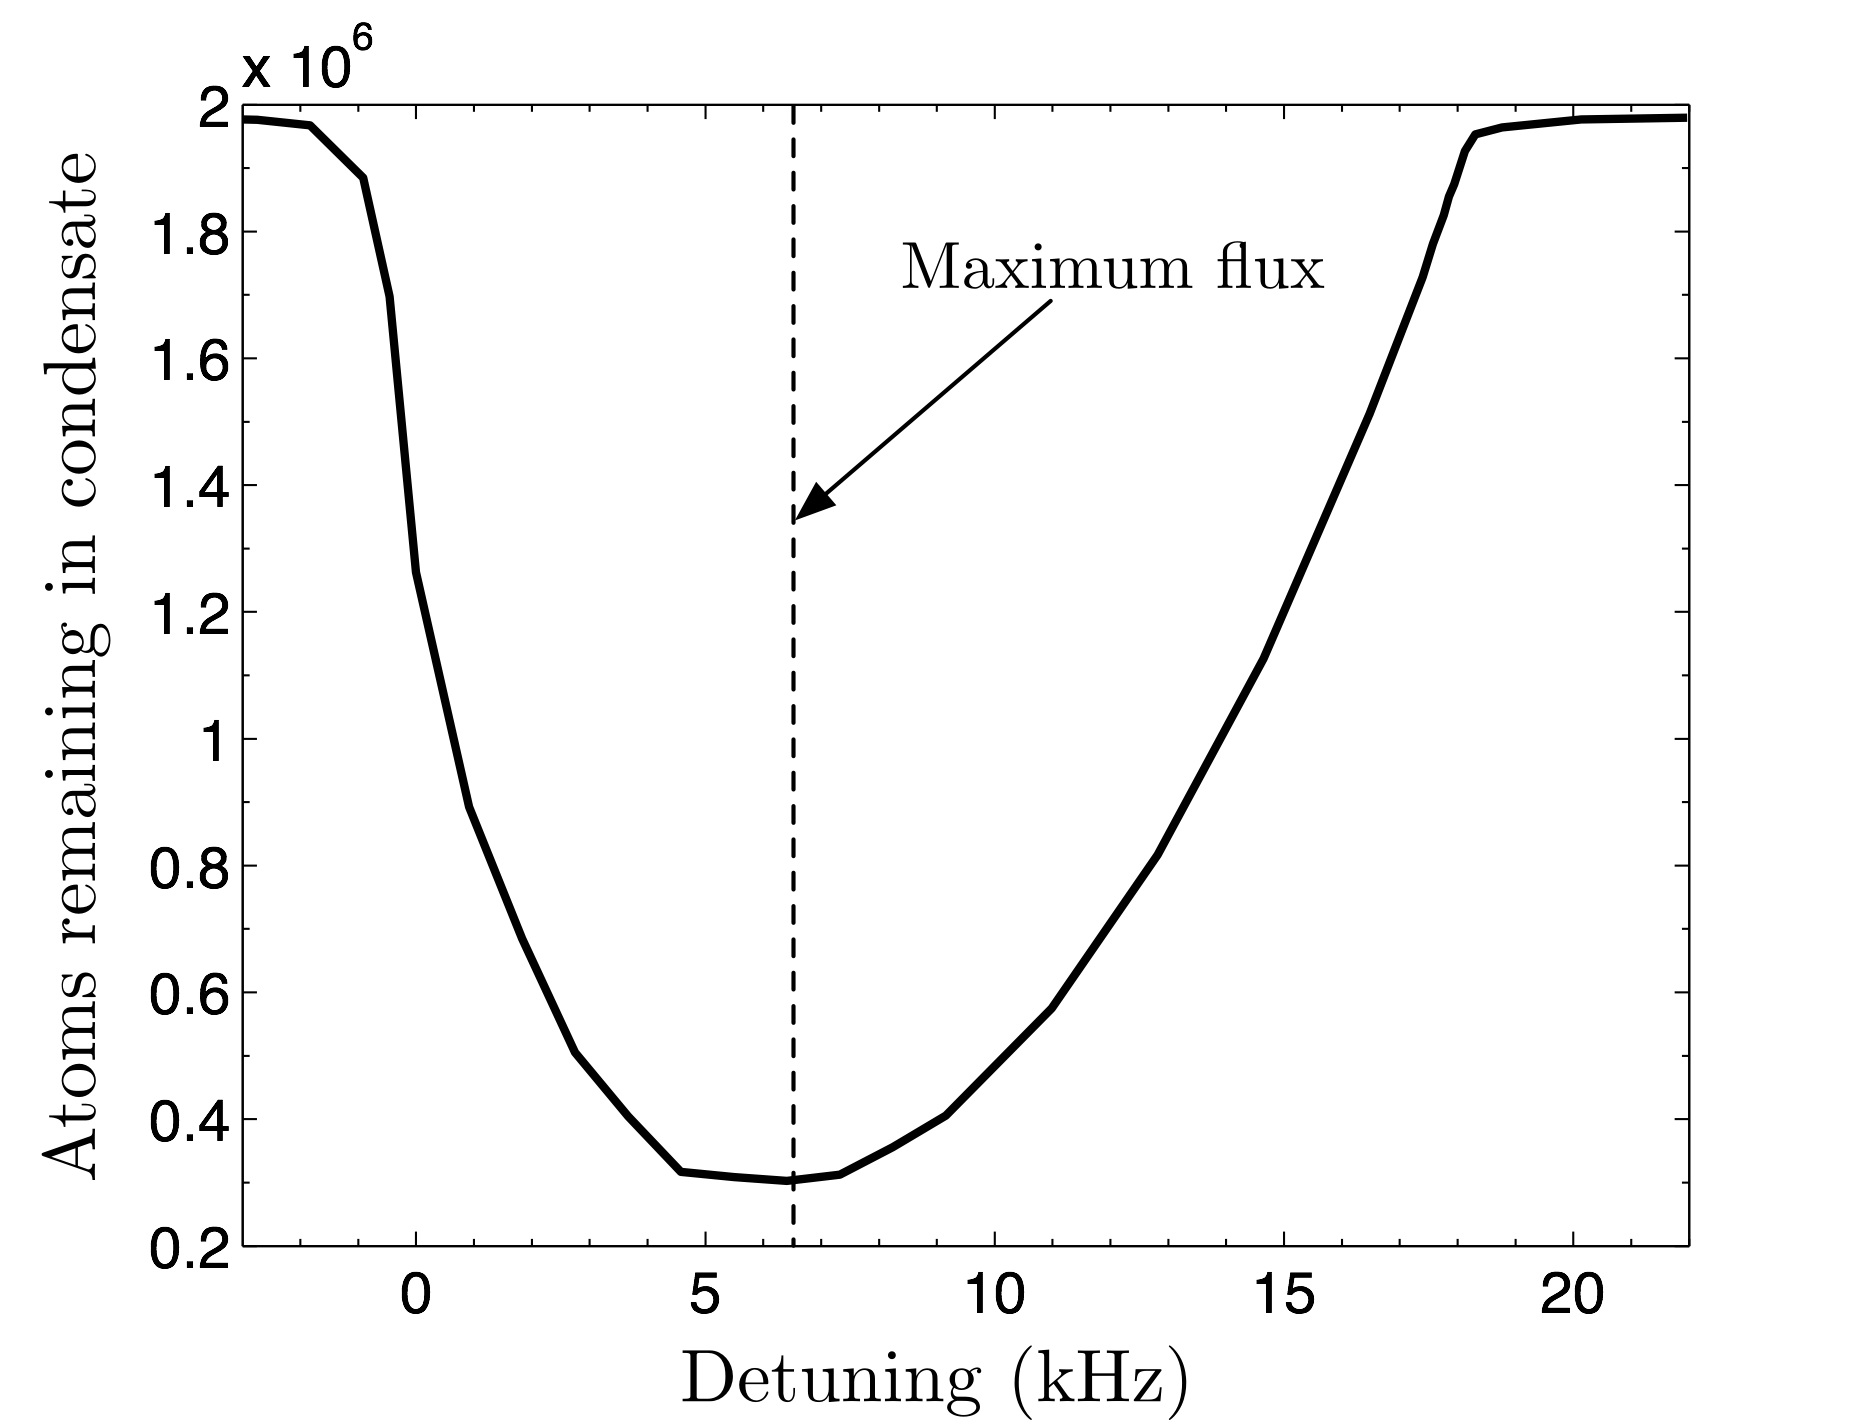
\includegraphics[width=8cm]{DetuningCurve}
    \caption{Theoretical calculation of the number of atoms remaining in the condensate after $\unit[10]{ms}$ of outcoupling at a Rabi frequency of $\Omega = \unit[210]{Hz}$ as a function of the detuning of the rf outcoupling from the centre of the condensate. The results shown are obtained from simulations of the 3D GP equations for the condensate under consideration. \label{Peaks:DetuningCurve}}
\end{figure}

\begin{figure}
    \centering
    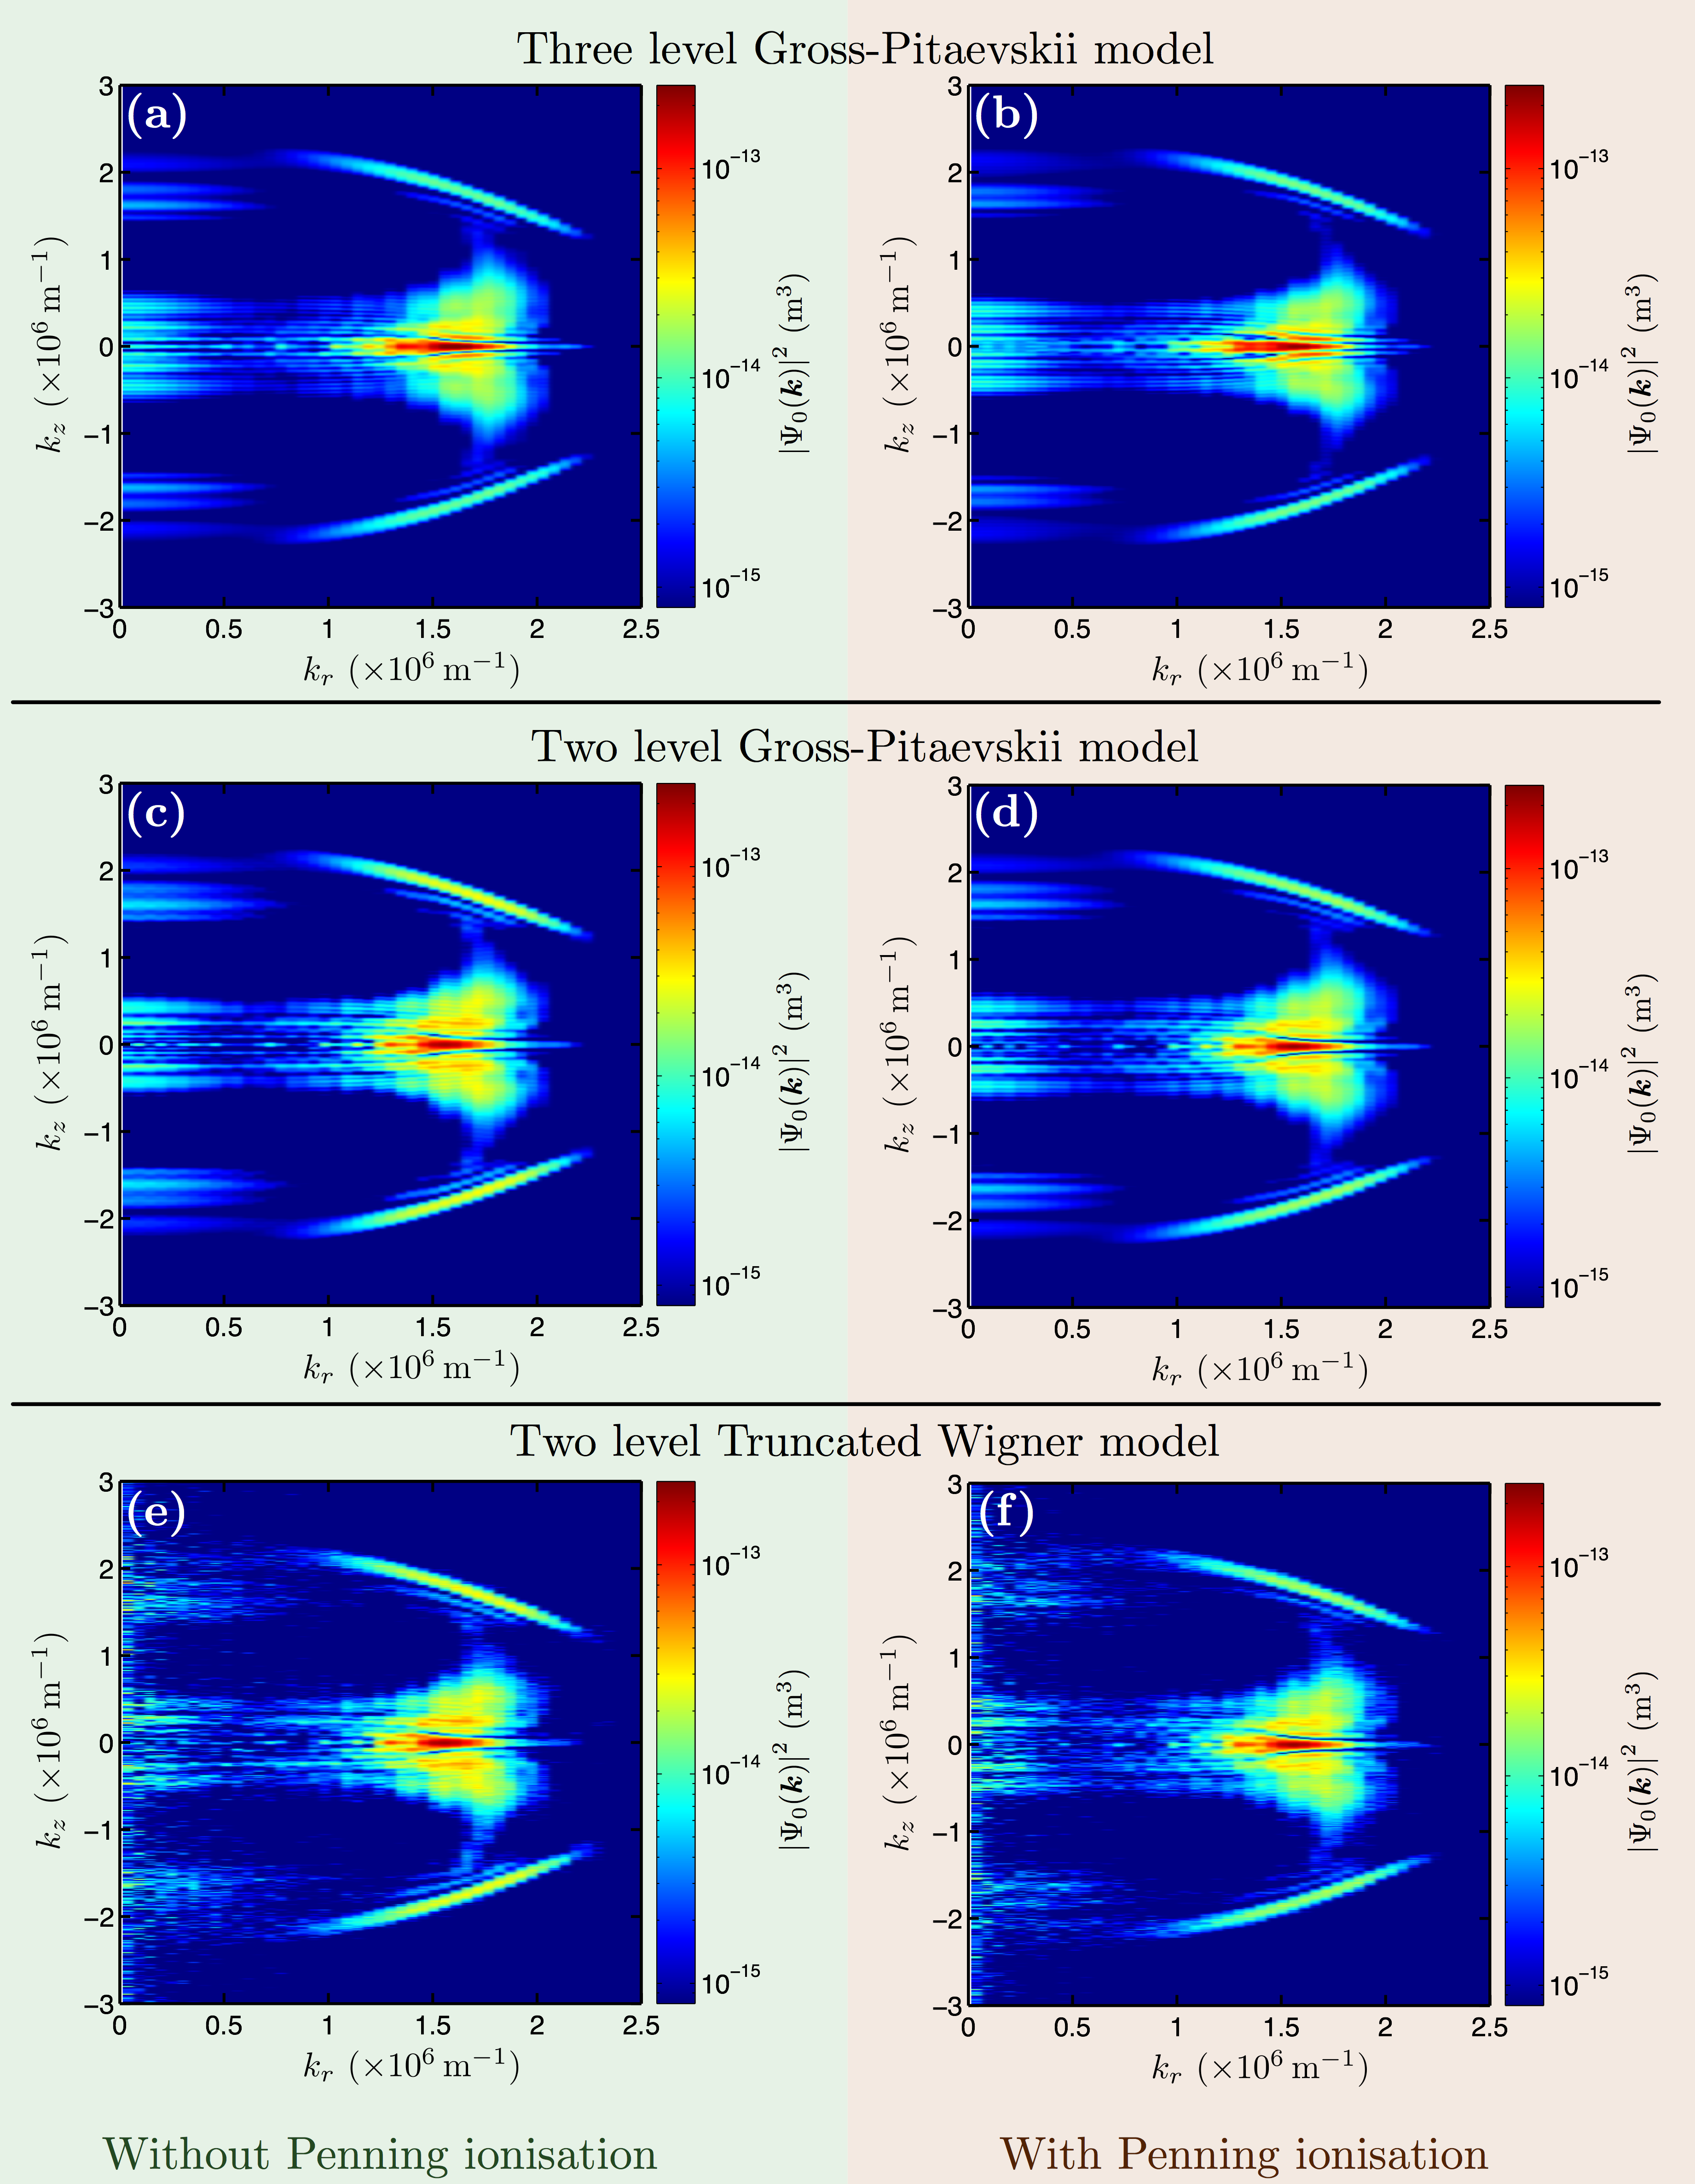
\includegraphics[width=14cm]{DetunedOutcouplingModelComparison}
    \caption{Simulation results for outcoupling with a detuning of $\Delta = 2\pi \times \unit[6.5]{kHz}$ from the centre of the condensate, with and without including the effects of Penning ionisation (right and left columns respectively). The upper figures (a) and (b) plot the results of a GP model including all $m_F$ atomic levels. Middle figures (c) and (d) plot the results of a reduced GP model where the $m_F=-1$ is assumed negligible, lower figures (e) and (f) correspond to a Truncated Wigner simulation for the same system with $N_\text{realisations} = 4$. The negligible difference between the figures in the left and right columns indicate that Penning ionisation has a negligible impact in the simulations depicted.\label{Peaks:TheoryMaxFluxDetuningResults}}
\end{figure}

The results of 2-level TW and 2- and 3-level GP simulations of the experiment for a detuning of $\Delta = 2\pi \times \unit[6.5]{kHz}$ are shown in \figureref{Peaks:TheoryMaxFluxDetuningResults}. As discussed at the end of \sectionref{Peaks:3DEquationsOfMotion}, a 3-level TW model is too computationally demanding to simulate, although the similarity of the results of the three models presented in \figureref{Peaks:TheoryMaxFluxDetuningResults} suggests that the results of such a simulation would differ negligibly from those presented.

The results pictured in \figureref{Peaks:TheoryMaxFluxDetuningResults} are of the momentum density $\abs{\Psi_0(\bm{k})}^2$ of the $m_F=0$ untrapped state at $t=\unit[5.1]{ms}$.  A comparison of the results of simulations with and without Penning ionisation are also shown (right and left columns respectively), which demonstrate that the features depicted are not suppressed by Penning ionisation.  As expected, the features of the momentum density profiles in \figureref{Peaks:TheoryMaxFluxDetuningResults} have a similar form to those in \figureref{Peaks:TheoryZeroDetuningNoPIResults}(c).  An important difference is that for detuned outcoupling, the features at large $\abs{k_z}$ appear in both the TW and GP models indicating that these structures are \emph{not} spontaneously seeded.  \figureref{Peaks:DetunedPeaksFormationProcess} illustrates the formation process of these structures demonstrating that they are produced by a stimulated scattering process from the condensate that sweeps in momentum from $k_z=0$ towards the final state pictured in \figureref{Peaks:TheoryMaxFluxDetuningResults}. 

\begin{sidewaysfigure}
    \centering
    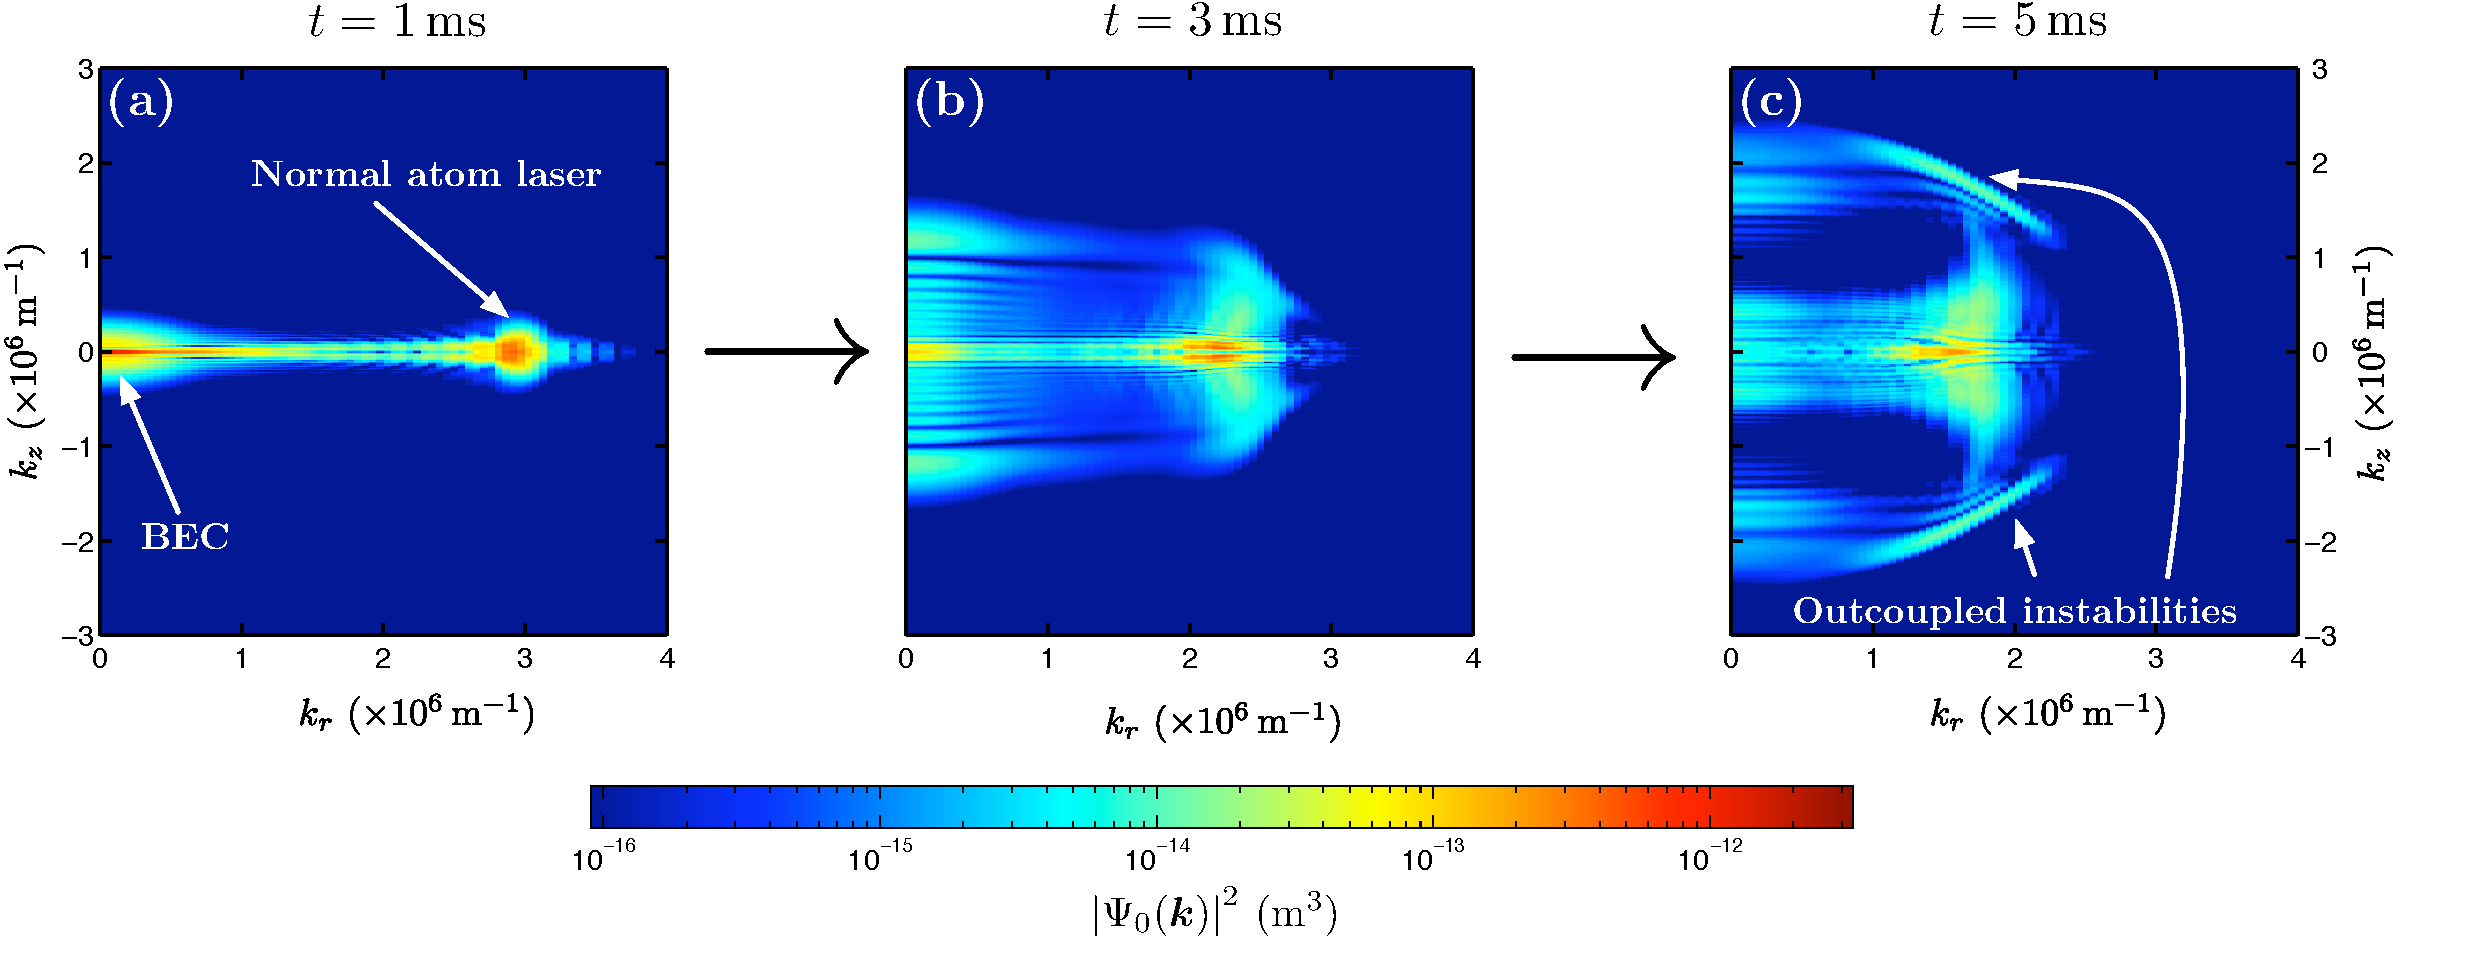
\includegraphics[width=20cm]{DetunedPeaksFormationProcess}
    \caption{Simulation results illustrating the formation of the peak-like structures due to stimulated scattering from the condensate. The results presented are from a three level GP model with a detuning of $\Delta = 2\pi \times \unit[6.5]{kHz}$ and include Penning ionisation (the results correspond to \figureref{Peaks:TheoryMaxFluxDetuningResults}(b)). Figures (a), (b), and (c) show the momentum density distribution $\abs{\Psi_0(\bm{k})}^2$ of the $m_F=0$ untrapped state at times \unit[1]{ms}, \unit[3]{ms}, and \unit[5]{ms} respectively. The marked outcoupled instabilities are the origin of the structure away from the main atom laser profile in \figureref{Peaks:ExpTheoryComparison}(e) and (f).
    \label{Peaks:DetunedPeaksFormationProcess}}
\end{sidewaysfigure}

A comparison between the experimental atom laser profile and the results of the 3-level GP simulations are presented in \figureref{Peaks:ExpTheoryComparison}.  The theoretical simulations are in excellent agreement with the experiment demonstrating that the instabilities discussed in \sectionref{Peaks:PerturbativeApproach} are the origin of the observed experimental atom laser profile.  The observed halo between the main atom laser profile and the peak-like structures at the upper and lower ends of the MCP profile are caused by the sweeping of the stimulated scattering process pictured in \figureref{Peaks:DetunedPeaksFormationProcess}.  Initially, the atom laser has negligible momentum in the weak trapping dimension ((a) of \figureref{Peaks:DetunedPeaksFormationProcess}).  This forms the central component to the atom laser profile in \figureref{Peaks:ExpTheoryComparison}(f).  As outcoupling continues the stimulated scattering process excites higher momentum modes in the axial dimension which are then outcoupled [\figureref{Peaks:DetunedPeaksFormationProcess}(b) and (c)] to form the background halo in \figureref{Peaks:ExpTheoryComparison}(f).  Once the stimulated scattering process stabilises at a maximum axial momentum, the peaks furthest from the central atom laser profile in \figureref{Peaks:ExpTheoryComparison}(f) become emphasised.

\begin{figure}
    \centering
    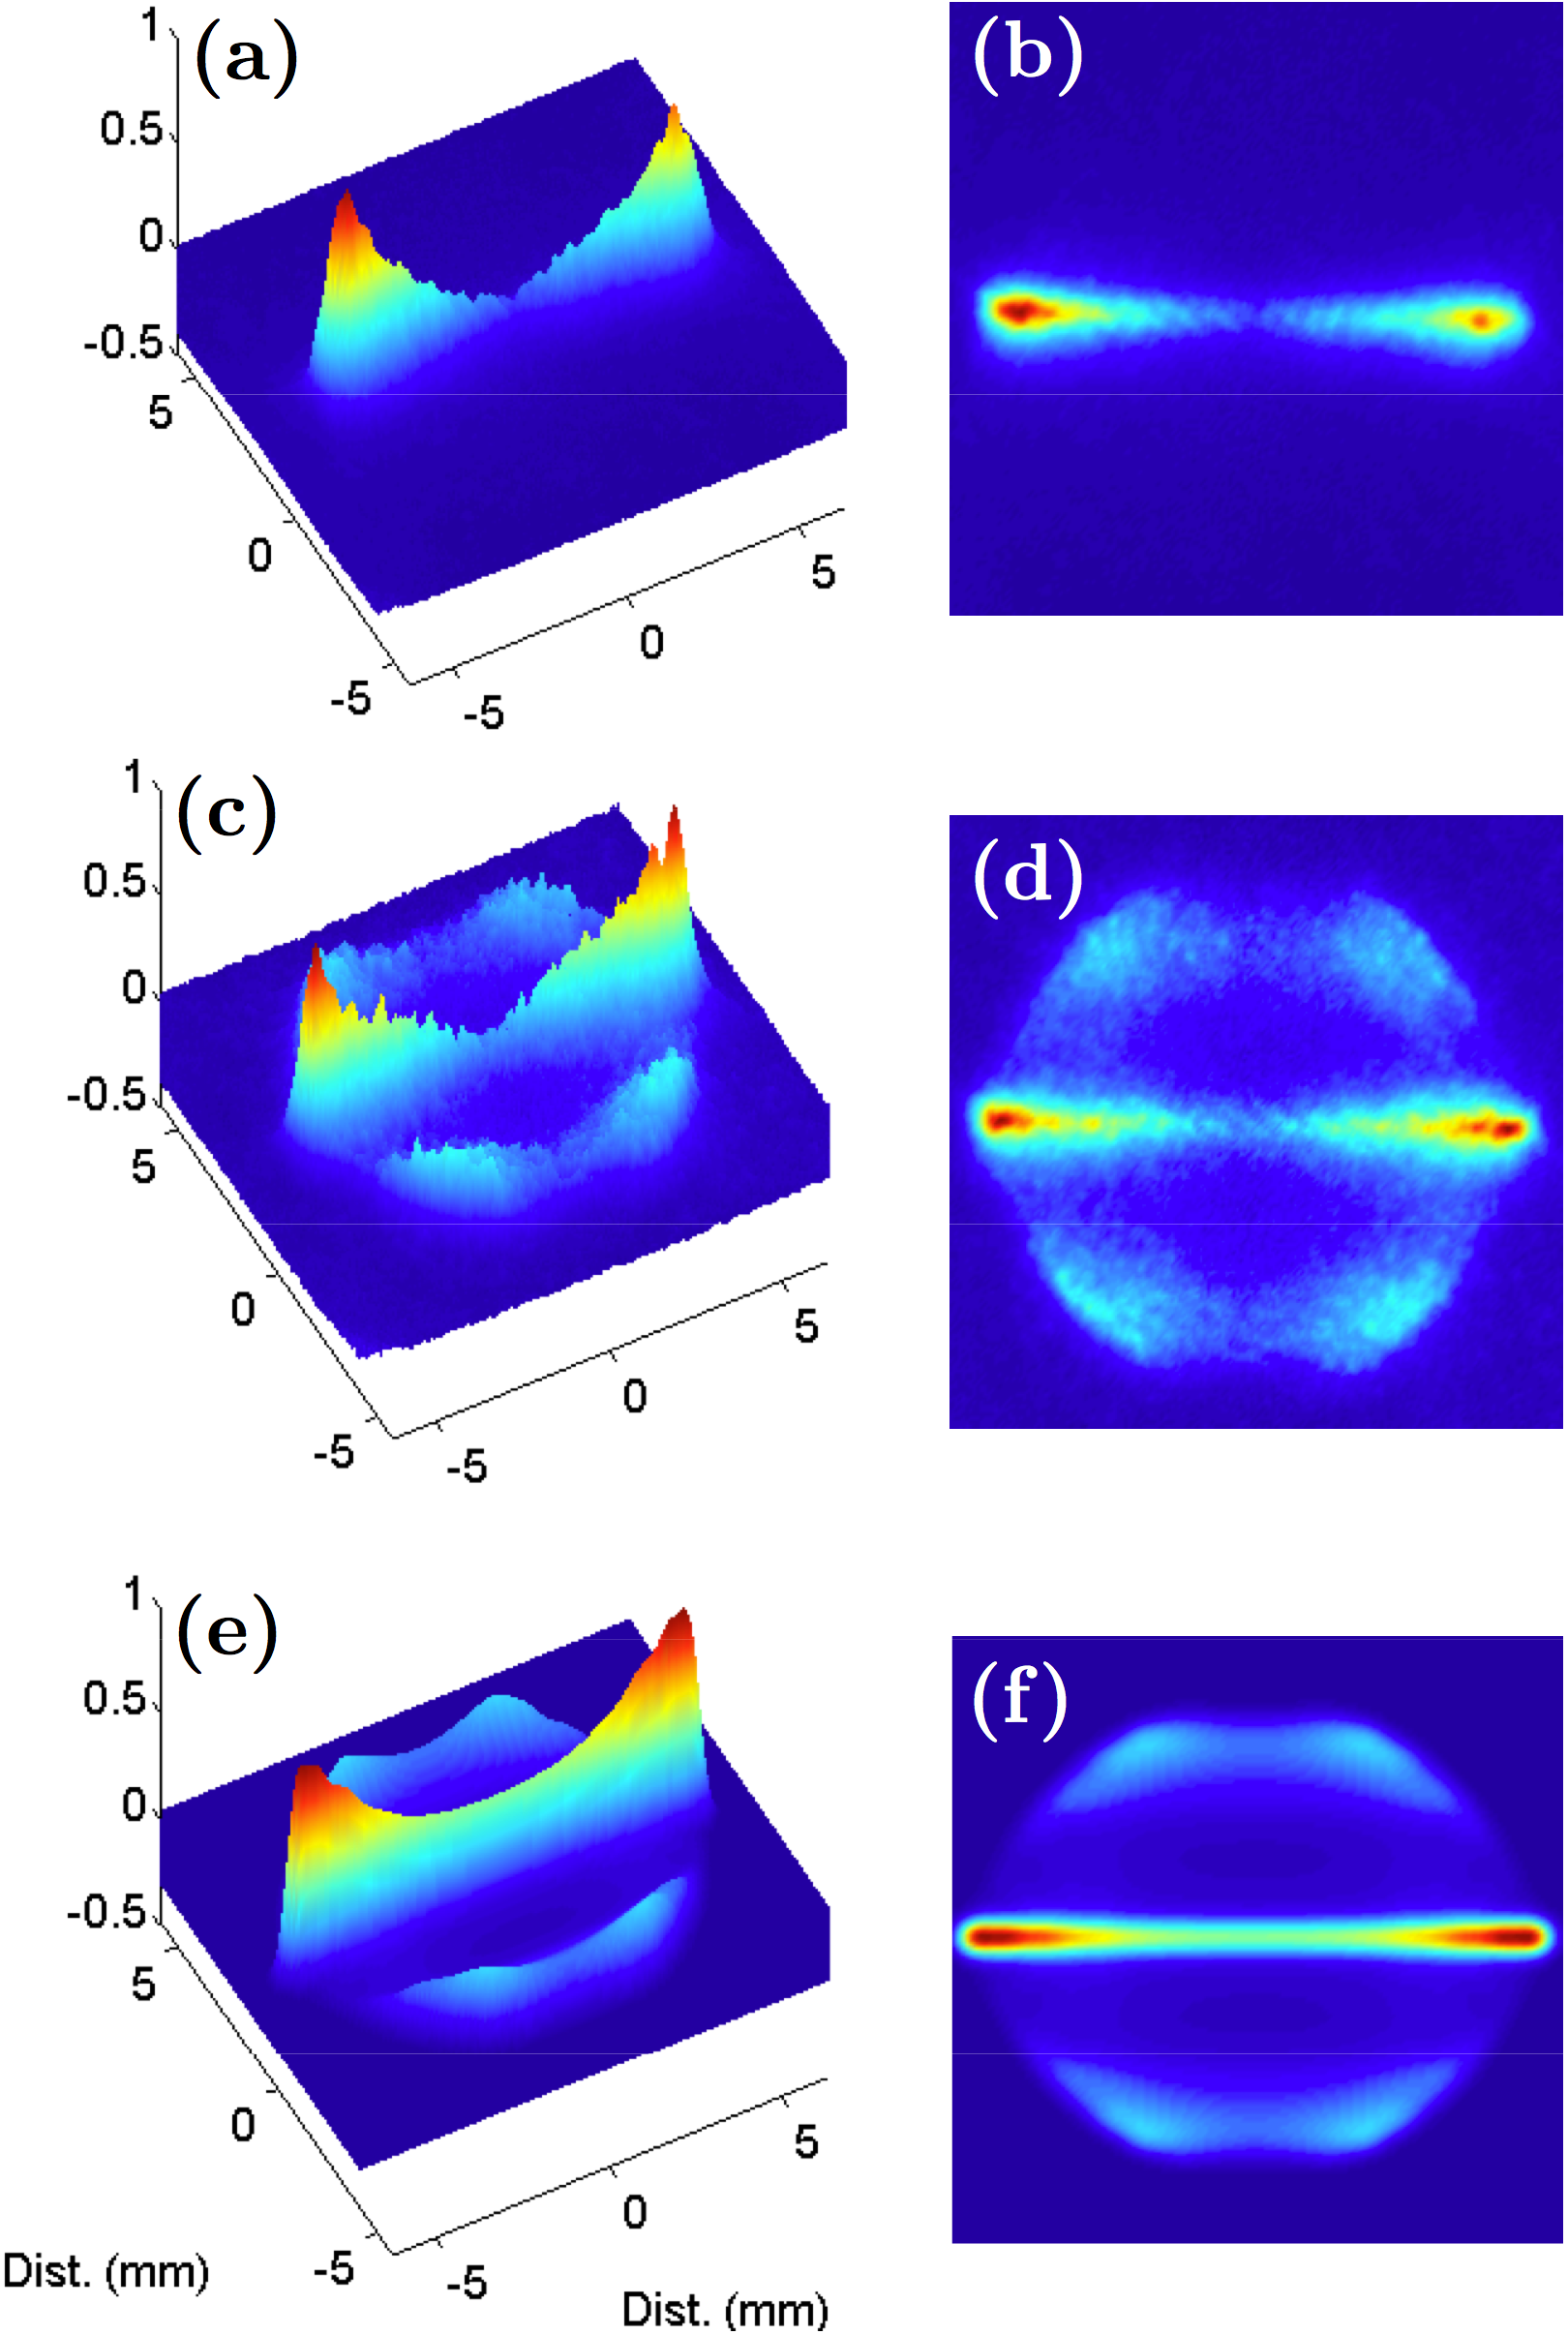
\includegraphics[width=8cm]{ExpTheoryComparison}
    \caption{First two rows show experimental atom laser spatial profiles on the MCP \unit[4]{cm} below the trap, in a three-dimensional rendering (left) and a two-dimensional image (right). Both sets of data were taken for an outcoupling detuning of \unit[6.5]{kHz}; however, the Rabi frequency is increased by an order of magnitude between the two sets. The upper row shows the usual He* atom laser (see \sectionref{TransverseProfile:Helium}), while the middle row demonstrates the appearance of the resonant scattering peaks. The bottom row is the result of a simulation of the second experiment. The weak axis of the trap is aligned along the vertical axis of the images on the right.\label{Peaks:ExpTheoryComparison}}
\end{figure}

\subsection{Entangled beams?}

The dynamical instabilities do not need to be spontaneously seeded to be EPR-entangled.  As discussed in \sectionref{FloquetAppendix:EPREntanglement}, the optical parametric down-conversion process that drives the formation of the instabilities gives rise to EPR-entanglement even in the case that one or both of the amplified modes are initially in non-vacuum initial states.  In this case the entanglement only exists after a finite delay time.  

Although it does not follow that the outcoupled instabilities pictured in \figureref{Peaks:ExpTheoryComparison} are not entangled simply because they are predicted by the GP equation, neither can it be concluded that they are.  Certainly it cannot be checked by using a GP model, however many more simulation realisations than were used for the TW simulations presented in \figureref{Peaks:TheoryMaxFluxDetuningResults} would be necessary to verify whether or not the instabilities are entangled.  This calculation is currently infeasible as each realisation takes approximately 20 CPU-hours, and well over 1000 realisations would be necessary.  

In the case of resonant outcoupling, the excellent agreement between the results pictured in \figureref{Peaks:ResonantOutcouplingProcess} with the semianalytical model of \sectionref{Peaks:PerturbativeApproach} suggests that we can be confident that the instabilities are entangled upon formation.  The outcoupling process itself would complicate the shape of the entangled modes essentially precluding the use of this mechanism for the direct detection of entangled atomic matter waves (even if atom local oscillators in the correct states could be constructed).  That said, for both resonant and detuned outcoupling number-difference squeezing between opposite sides of the MCP detector should be robust enough to survive outcoupling.  These correlations will only exist in the time-integrated profiles as it will not be possible to determine when the other atom in the pair should arrive on the other side of the detector as the process discussed in this chapter is continuous, and hence a space-time reconstruction of the momentum distribution such as that performed in \citep{Perrin:2007} is not possible.

Although it was not possible to investigate the existence of number-difference squeezing in the experiment described in this chapter, a recent upgrade to the experimental apparatus to include a high-resolution detector similar to that used by \citet{Perrin:2007} has made this a possibility.  The author is hopeful that an experiment to look for the predicted number-difference squeezing will be performed in the near future.

\section{Summary}

In this chapter an unusual process in an atom laser was investigated.  The process involved the direct conversion of mean-field energy to the kinetic energy of unstable modes in the condensate.  This process was shown to generate entanglement in certain regimes, although in the experiment discussed it is unlikely that this entanglement remains in the outcoupled atom laser, and certainly not in any useful form.  These problems are however not fundamental.  A differently-designed experiment could overcome some of these problems to potentially produce entangled atom lasers.

One possibility worthwhile investigating would be to use a highly elongated two-state condensate in which both states experience the same trapping potential.  This could be achieved for example through the use of an optical dipole trap, or by trapping the $F=1$, $m_F=-1$ and $F=2$, $m_F=1$ \nucl{87}{}{Rb} states in the same magnetic trap.  As the two states of the condensate experience the same trapping potential, the two components of the dynamical instabilities would propagate together avoiding the problem of one of the components of the entangled modes leaving the condensate without the other.  Further, due to the high aspect ratio, the instabilities would propagate solely along the axial dimension.  To extract the entangled beams, one could ensure that the kinetic energy of the instabilities was higher than the trapping potential in the case of an optical dipole trap, or turn off the magnetic trap to allow the entangled beams to expand ballistically and separate from the condensate in the axial direction.  This experiment may then enable the production of highly-directional entangled atom lasers that would also be continuous in the case of the optical dipole trap.  Further theoretical investigation would be necessary to determine if such an experiment were feasible.

\parasep

\begin{quote}
    \emph{The most exciting phrase to hear in science, the one that heralds new discoveries, is not ``Eureka!'' but ``That's funny\dots''} --- Isaac Asimov
\end{quote}

The interaction between theory and experiment is a two-way street.  As a theorist, one might like to think that you can simply do some calculations, make some interesting predictions and then try to convince an experimentalist to test them.  While this is certainly a large part of the interaction, it sometimes goes the other way.  Sometimes the experimentalist tries something and the results show something that she didn't expect. ``That's funny,'' says the experimentalist.  She shows the results to the theorist and asks what might be going on.  ``That's funny,'' says the theorist\dots

This chapter has presented the results of one such interaction.  While they are not a major discovery by any stretch of the imagination, they are a testament to the accuracy of the theoretical techniques available for describing Bose-condensed systems that experimental results as strange as those presented in \figureref{Peaks:ExpTheoryComparison} can be accurately explained by theoretical calculations.




\chapter{Optical pumping of an atom laser}
\label{OpticalPumping}
\graphicspath{{Figures/OpticalPumping/}{Figures/Common/}}

The results presented in this chapter have been published in~\citet{Robins:2008,Doring:2009}.

\section{Motivation}

The development of the continuous-wave optical laser was a significant advance over the first pulsed ruby laser. The continuous-wave optical laser opened up many applications. The atom laser is a very promising source for both precision measurement and fundamental physics.

The replenishment process can be divided into two critical components: a delivery system for filling an atomic reservoir with ultracold atoms and a pumping mechanism for irreversibly and continuously transferring atoms from the reservoir to the laser mode.

The technical requirements on both parts of the replenishment system are stringent. Nonetheless, recent experiments have demonstrated that a delivery system for atoms is feasible and possible.~\citet{Chikkatur:2002qa} showed that Bose-condensed atoms could be periodically transported over large distances using a moving optical dipole trap. Further experiments with transport, based on interference of two counter-propagating lasers, have shown that dipole trapping techniques could be extended to provide continuous delivery of atoms~\citep{Schmid:2006}. Magnetic guiding systems for ultracold atoms may also provide a path to future delivery systems~\citep{Lahaye:2004,Greiner:2001,Greiner:2007}.

The realisation of the pumping mechanism for a continuous atom laser has proved more problematic. There are four critical requirements that are difficult to satisfy experimentally. First, the atoms should enter the laser mode continuously and coherently, that is, with the phase and amplitude of the lasing condensate. Thus, atoms must make a transition that is Bose-stimulated by the atomic lasing mode. The second requirement is that the pumping process is irreversible. It requires coupling to a reservoir. There are two reservoirs available, the empty modes of the electromagnetic field accessible via a transition from an excited atomic state, or the empty modes of the atomic field accessible via evaporation. For a high-coherence atom laser, the lasing mode must be a pure condensate with a significantly smaller thermal fraction, making evaporation-induced pumping a difficult possibility for the production for a highly coherent continuous atom laser. The third requirement is that the pumping system must be compatible with a continuous replenishment mechanism. This suggests strongly that there be a physical separation between the source and the lasing condensates. A physical separation with a stimulated transition between the source and the lasing mode isolates the lasing mode from phase kicks and heating that would result either as a necessary consequence of the replenishment system (for example in the replenishment system demonstrated by~\citet{Chikkatur:2002qa} where condensates are merged) or as a consequence of an imperfect delivery system. Finally, the fourth condition on a pumping system is that it should be possible to continuously output-couple atoms from the laser mode into a beam, while the pumping mechanism is operating.

The two possibilities for reservoirs to supply the irreversibility necessary for the proper operation of a pumped atom laser (Bose-Einstein condensate) are considered in this chapter and the next. In this chapter, pumping an atom laser using interactions mediated by light is considered. In this case the reservoir providing the irreversibility are the vacuum electromagnetic modes into which light is scattered by the pumping process. \chapterref{KineticTheory} considers the alternate possibility of using atomic \emph{s}-wave scattering interactions to mediate the pumping process with evaporation to make the process irreversible.

\hrule

Previous work on light-BEC interactions. Rayleigh/Raman superradiance, EIT, CARL, and the rest of that list that I had.


\section{Pumping mechanism}
\label{OpticalPumping:PumpingMechanism}

\begin{figure}
    \centering
    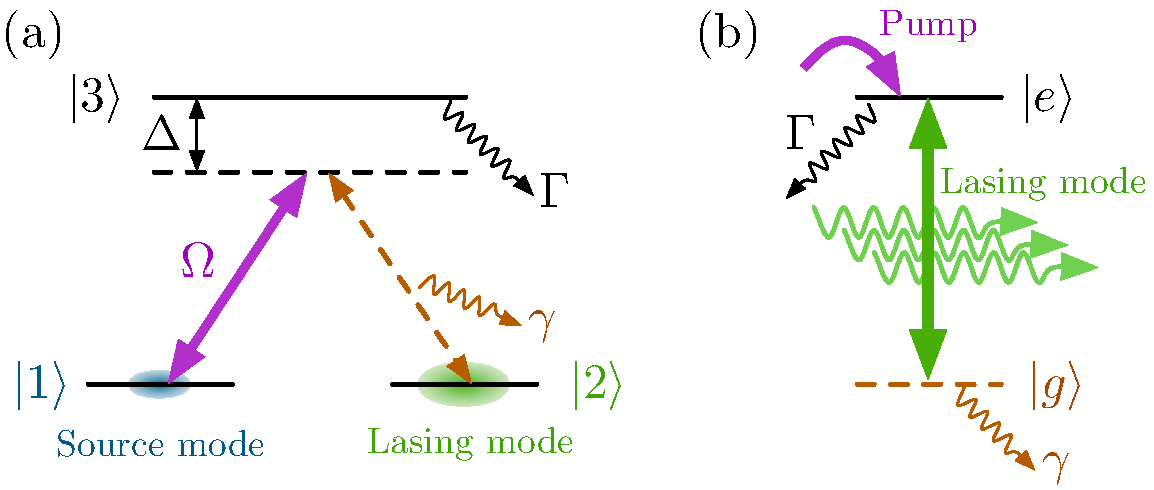
\includegraphics[width=14cm]{LambdaModel}
    \caption{FIXME: This is not a caption. Comparison of considered atom laser pumping scheme (a) and typical optical laser pumping scheme (b).\label{OpticalPumping:LambdaModel}}
\end{figure}

The optical pumping process under investigation in this chapter is illustrated in \figureref{OpticalPumping:LambdaModel}(a).  In this process atoms in the source mode are driven by a laser into an excited state from which they can decay into the lasing mode (the condensate).  Although there is no laser driving this second transition ($\ket{3}\leftrightarrow\ket{2}$), the decay of atoms into the lasing mode is not spontaneous emission in the usual sense.  The emission process is \emph{atomically}-stimulated by the large occupation of the lasing mode in the same way that the transition may be \emph{optically}-stimulated even in the absence of any population in the atomic state into which the atom decays.

The final decay of an atom into the lasing mode in \figureref{OpticalPumping:LambdaModel} resembles standard \emph{optical} laser schemes [see \figureref{OpticalPumping:LambdaModel}(b)] in which the roles of atoms and light are reversed.  In an optical laser an atom in the excited state is stimulated to emit into the ground state by the resonant photons in the laser cavity.  Once the atom has emitted, it decays rapidly into other internal states with rate $\gamma$ significantly limiting reabsorption from the $\ket{g}$ state.  A similar process occurs in the proposed optical pumping scheme in which the photon emitted as the atom decays  leaves the system rapidly preventing reabsorption.  The loss of photons from the system is represented by the decay of the optical mode with rate $\gamma$ in \figureref{OpticalPumping:LambdaModel}(a).

This similarity between the proposed atom laser pumping mechanism and the usual optical laser pumping mechanism is clearly illustrated by considering the Hamiltonian coupling the excited and ground atomic states in \figureref{OpticalPumping:LambdaModel}
\begin{align}
    \hat{H} &= \hbar \epsilon \left(\hat{a}_e^\dagger \hat{a}_g \hat{a}_\text{ph} + \hat{a}_g^\dagger \hat{a}_\text{ph}^\dagger \hat{a}_e  \right),
    \label{OpticalPumping:TwoLevelAtomHamiltonian}
\end{align}
where $\epsilon$ is a real coupling constant, the $\hat{a}_e$, $\hat{a}_g$, and $\hat{a}_\text{ph}$ are annihilation operators for the atomic excited state, atomic ground state and photon mode respectively.  The rotating wave approximation has been made in obtaining this Hamiltonian, assuming that the optical mode is not detuned from the atomic transition by a large fraction of the frequency difference between the two states.  

The Hamiltonian \eqref{OpticalPumping:TwoLevelAtomHamiltonian} describes both the atom- and optical-laser pumping mechanisms, the difference in the mechanisms being in the occupations of the various states.  If the system is initially in a state with $N_e$ atoms in the atomic excited state, $N_g$ atoms in the atomic ground state and $N_\text{ph}$ photons in the optical mode, the amplitude for an atom in the excited state to emit a photon is
\begin{align}
    \bra{N_e-1, N_g + 1, N_\text{ph} + 1} \hat{H} \ket{N_e, N_g, N_\text{ph}} &= \hbar \epsilon \sqrt{N_g+1} \sqrt{N_\text{ph}+1} \sqrt{N_e}.
\end{align}
This emission process can therefore be stimulated either by photons ($N_\text{ph} > 0$) or by atoms ($N_\text{g} > 0$).  It would also be possible for the emission to be stimulated by both photons \emph{and} atoms, although in this case the amplitude for the absorption process would be non-zero
\begin{align}
    \bra{N_e+1, N_g - 1, N_\text{ph} - 1} \hat{H} \ket{N_e, N_g, N_\text{ph}} &= \hbar \epsilon \sqrt{N_e+1} \sqrt{N_\text{ph}} \sqrt{N_g}.
\end{align}
It is for this reason that it is desirable in an optical laser to have $N_g \approx 0$, and in the proposed atom laser pumping scheme to have $N_\text{ph} \approx 0$.

Atom laser pumping schemes of the form of that illustrated in \figureref{OpticalPumping:LambdaModel}(a) have been proposed before~\citep{Olshanii:1996,Janicke:1996,Spreeuw:1995,Cirac:1996rr,Cirac:1996,Santos:2000,Castin:1998,Cirac:1994,Vengalattore:2003,Santos:2001ve,Wolf:2000,Santos:1999qf} for the production of BEC without the use of collisional evaporation and its consequent losses.  The main problem that they all seek to address is that of reabsorption of photons spontaneously emitted when the atom in state $\ket{3}$ decays to the $\ket{2}$ state, but not to the lasing mode.  This emitted photon will be resonant with the lasing mode and may be scattered several times before finally leaving the condensate.  A single such spontaneously emitted photon can cause significant heating of a condensate as the single photon recoil energy can be as large as or greater than the chemical potential of the condensate.

One proposed method~\citep{Castin:1998,Vengalattore:2003} for reducing the heating uses a purely geometric solution: if a condensate is made sufficiently narrow in one or more dimensions such that a photon emitted in one of those directions is negligibly likely to be reabsorbed, the overall probability for reabsorption will also be reduced.  While this method may be appropriate for the initial formation of BEC, it is impractical for a large BEC as the trap deformation necessary to reach the required regime is extreme.  For a \nucl{87}{}{Rb} condensate of $N= 5\times 10^5$ atoms with trapping frequencies of $\omega_x = \omega_y = \unit[2\pi \times 128]{Hz}$, $\omega_z = \unit[12.8]{Hz}$, the mean-free path in the centre of the condensate for a resonant photon on the cycling transition ($\lambda = \unit[780]{nm}$) is $1/(n \sigma) = \unit[16]{nm}$ where $n$ is the peak condensate density and $\sigma = 3 \lambda^2/2 \pi$ is the atomic scattering cross-section.

Another possibility for reducing reabsorption that works well in optical lattices is to operate in the \emph{festina lente} regime~\citep{Wolf:2000,Santos:1999qf,Cirac:1996,Castin:1998} in which the energy levels of the trap are sufficiently separated such that a photon emitted when an atom decays into a particular trap level is only resonant with atoms in that level (and those levels degenerate with it).  This prevents the occurrence of `dangerous' processes in which an excited atom decays into a non-condensate level with the emitted photon being absorbed by the condensate.  In the case of resonant optical pumping light ($\Delta = 0$ in \figureref{OpticalPumping:LambdaModel}(a)), the \emph{festina lente} regime requires that $\omega_\text{min} \gg \Gamma$  where $\omega_\text{min}$ is the minimum of the magnetic trapping frequencies.  Strictly, the \emph{festina lente} regime has only been investigated in the absence of \emph{s}-wave scattering interactions, however one would expect that in the presence of \emph{s}-wave scattering the trap frequency energy scale would simply be replaced by the energy of the relevant Bogoliubov excitation (refer to \sectionref{Peaks:ElementaryExcitations}).  Regardless, the \emph{festina lente} regime is impractical to achieve in alkali gases like \nucl{87}{}{Rb} as the relevant decay rate is $\Gamma = \unit[2\pi\times 5.9]{MHz}$, which is much larger than typical trap frequencies ($\omega \sim \unit[2\pi \times 100]{Hz}$) and condensate excitations ($\mu/\hbar \sim \unit[2\pi \times 10]{kHz}$).

A third possibility for reducing reabsorption is to operate in the \emph{boson accumulation regime} (BAR)~\citep{Cirac:1996rr,Floegel:2001} in which an atom in the excited state is significantly more likely to decay into the condensate mode than into all other modes.  In this limit it can be shown that absorption of emitted photons by atoms not in the condensate mode can be neglected.  It is in the BAR that we wish to operate our proposed pumping mechanism of \figureref{OpticalPumping:LambdaModel}(a).  

Up to this point, the source mode was entirely arbitrary; without consideration of reabsorption the proposed pumping process would work equally well for coherent or thermal states in the source mode.  As the optical transition between the excited atomic state and the lasing mode is not driven by a laser, the phase of the photons emitted is determined by the relative phase between the source and lasing modes; the direction of population transfer does not depend on the phase difference between these two modes. However the requirement that excited atoms be significantly more likely to decay into the condensate mode than to any other mode places a stringent requirement on the source mode of the pumping mechanism.  For this requirement to be satisfied, the momentum width of the source atom distribution cannot be significantly larger than the momentum width of the condensate.  If this were not the case a significant fraction of the atoms would not be momentum-resonant with the condensate under the pumping process and will therefore not be in the boson accumulation regime.  These atoms would be able to reabsorb spontaneously emitted photons causing the reabsorption problem previously discussed.  For an atomic distribution to have a momentum width comparable to that of the target condensate, the atoms must either be condensed or if they are thermal, be trapped in a significantly weaker trap than the target condensate mode and have a temperature below the condensation temperature in the tighter trap.  

Although it would be desirable to be able to use a thermal source of atoms as the source mode, the remainder of this chapter will investigate the possibility of using a coherent source of atoms as the source mode of the pumping mechanism.  Specifically, this coherent source will be an atom laser extracted from a second, source condensate.  Continuous operation of this scheme could in principle be achieved by replacing the source condensate with an independently-produced condensate once it is depleted.  As the pumping mechanism is independent of the phase-difference between the source and lasing modes this will not affect the direction of population transfer.

% \parasep
% 
% The pumping mechanism described in this section bears some resemblance to other optical processes that can occur in Bose-Einstein condensates such as EIT, and Rayleigh/Raman superradiance. FIXME: Complete paragraph/s.
% 
% Quote from the paper:
% 
% The mechanism we have described for pumping is related to pulsed Raman super-radiance that has been studied previously.  In our work, in the laboratory frame, atoms are driven from the $\ket{2, 0}$ untrapped state into the $\ket{1, -1}$ trapped state enabling us to continue pumping indefinitely.  the condensate that we pump is stationary in the laboratory frame.  Furthermore, our experiment is carried out in a double-condensate geometry with internal states that enable simultaneous pumping and outcoupling to produce a freely propagating atom laser beam from a simultaneously pumped condensate.
% 
% There is a second mechanism that we have considered that is related to the EIT mechanism described in the work by~\citet{Ginsberg:2007fk}.  Similar to the existing Raman super-radiance experiments, their work was necessarily carried out in a pulsed regime.  In our experiment, again, the geometry and choice of internal states enable the possibility of carrying out a related experiment continuously.  The condensates in such an experiment must have some spatial overlap.  The $\ket{2, 0}$ atoms are produced in the overlap region where the $\pi$-polarised pump beam is absorbed and the $\sigma$-polarised beam is produced.  Both beams travel in the same direction.  The amplitude of the $\pi$-polarised beam decays in the overlap region.  The amplitude of the $\sigma$-polarised beam grows.  The atoms follow the dark state and are pumped continuously to the lasing mode.


\section{The continuous pumping experiment}
\label{OpticalPumping:ContinuousExperiment}

A summary is provided here of the continuous pumping experiment performed by \emph{Nick Robins}, \emph{Cristina Figl} and \emph{Matthew Jeppesen} at the Department of Quantum Science, ANU.  Further details of the experimental setup and results are published in \citet{Robins:2008}.

\begin{figure}
    \centering
    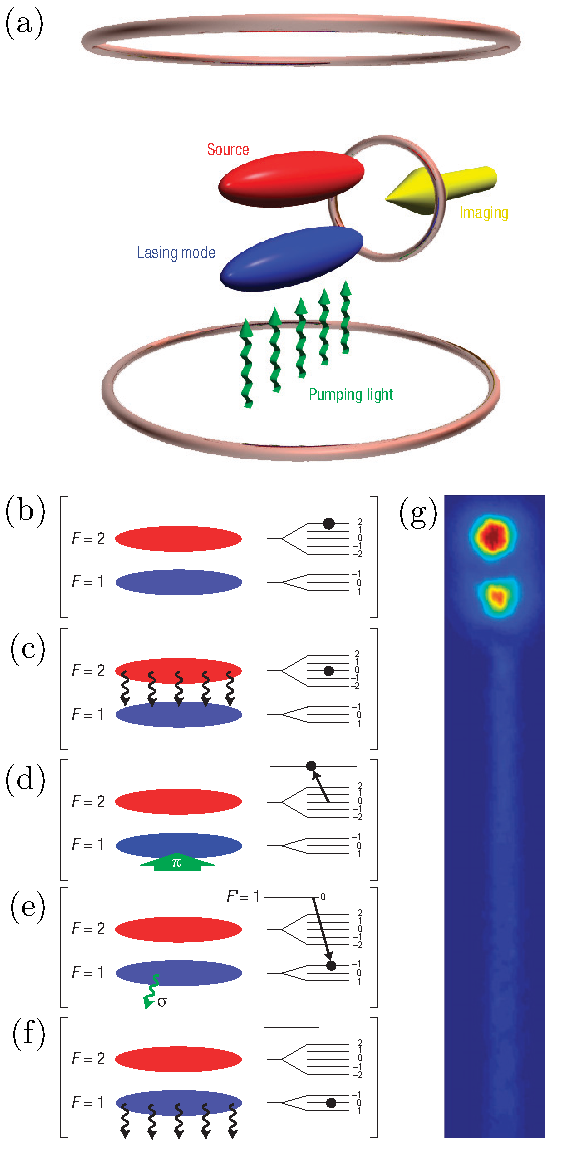
\includegraphics[width=8cm]{ExperimentSchematic}
    \caption{FIXME: Caption.  Schematic diagram of the operation of the pumped atom laser.  Schematic diagram of the experiment (a) and pumping steps (b--f).  A radiofrequency field spin-flips the atoms to the $\ket{2, 0}$ state (b), and they fall under gravity (c).  The light field couples the atoms to the $F'=1$ excited state from which they are stimulated to emit into the $\ket{1, -1}$ BEC.  The atomic momentum is cancelled by the absorption and emission of the photons (d, e).  A second radiofrequency field finally output-couples the atoms into the $\ket{1, 0}$ atom laser (f).  (g), Absorption image of the experimental system, showing source, laser mode and output beam.}
    \label{OpticalPumping:ExperimentSchematic}
\end{figure}

\begin{table}
    \centering
    \begin{tabular}{cc}
    \toprule
    Parameter & Value\\
    \midrule
    $\ket{F=2, m_F=2}$ (source) condensate number & $N_\text{source} = (6.7 \pm 0.5)\times 10^5$ \\
    $\ket{F=1, m_F=-1}$ (laser) condensate number & $N_\text{laser} = (5.0 \pm 0.4) \times 10^5$ \\
    Radial trapping frequency (for $\ket{1, -1}$) & $\omega_r = \unit[2\pi \times 130]{Hz}$ \\
    Axial trapping frequency (for $\ket{1, -1}$) & $\omega_z = \unit[2\pi \times 13]{Hz}$ \\
    \bottomrule
    \end{tabular}
    \caption{Experimental parameters for the Rubidium-87 BEC system under consideration.}
    \label{OpticalPumping:ExperimentalParameters}
\end{table}


To produce a pumped atom laser two independent condensates are prepared in the $\ket{F=2, m_F=2}$ and $\ket{F=1, m_F=-1}$ magnetically trapped states of \nucl{87}{}{Rb}.  Owing to their larger magnetic moment, the $\ket{2, 2}$ atoms are more tightly confined in the magnetic field than the $\ket{1, -1}$ atoms, and hence the evaporation does not directly cool them.  They are, however, sympathetically cooled through elastic collisions with the $\ket{1, -1}$ atoms~\citep{Myatt:1997}.  For the condensate numbers and trapping frequencies given in \tableref{OpticalPumping:ExperimentalParameters} the Thomas-Fermi radius of each cloud is approximately $\unit[5]{\micro m}$ in the vertical direction.  The different magnetic moments of the two clouds lead to a gravitational sag between their centres of $\unit[8]{\micro m}$. Hence, the two clouds of atoms overlap only slightly, with the $\ket{2, 2}$ source condensate located above the $\ket{1, -1}$ laser-mode condensate [see \figureref{OpticalPumping:ExperimentSchematic}(a)].

To measure the effect of pumping, it is essential that the number of atoms in each state is stable from one experimental run to the next.  For this purpose, many details of the apparatus were refined, including very efficient baffling against stray resonant light, very low uncertainty and drift in laser frequency, intensity and polarisation, and good vibrational and thermal stability of the trap.  The stability of the number of atoms in each state was determined for a data set comprising 20 measurements, and found to be as low as 1\%.

The operation of the experiment is illustrated in \figureref{OpticalPumping:ExperimentSchematic}.  Starting with an initial number of atoms in each state [\figureref{OpticalPumping:ExperimentSchematic}(b)], a weak continuous radiofrequency field is applied to the upper source cloud which couples atoms from the $\ket{2, 2}$ state, through $\ket{2, 1}$ to the $\ket{2, 0}$ state.  This coupling is highly spatially selective and does not affect the $\ket{1, -1}$ cloud.  These atoms begin to fall away from the $\ket{2, 2}$ source cloud [\figureref{OpticalPumping:ExperimentSchematic}(c)].  Simultaneously approximately $\unit[10]{pW}$ of upward propagating $\pi$-polarised light resonant with the $\ket{F=2}\rightarrow\ket{F'=1}$ transition is applied.  Although this light is resonant in energy with the $\ket{2, 2}$ source atoms, they are prevented from absorbing photons by atomic selection rules.  Hence, the source cloud is unaffected by the pumping light.  For pumping the laser mode, the $\ket{2, 0}$ atoms will absorb the pumping light [\figureref{OpticalPumping:ExperimentSchematic}(d)].  As these atoms fall, they may make a transition into the excited $\ket{F'=1, m_F=0}$ state from which they are stimulated to emit into the laser mode $\ket{1, -1}$ by the atoms already present in that mode [\figureref{OpticalPumping:ExperimentSchematic}(e)].  The $\sigma^{+}$-photon emitted in this process carries the phase difference between the pump atoms and the condensate.  Finally, the $\ket{1, -1}$ laser-mode atoms are output-coupled to produce the atom laser beam in the $\ket{1, 0}$ state [\figureref{OpticalPumping:ExperimentSchematic}(f)].  An absorption image of the ultracold atoms used to build the pumped atom laser system is shown in \figureref{OpticalPumping:ExperimentSchematic}(g).

For successful pumping, the pump atoms must be momentum-resonant with the lasing condensate.  This means that their atomic velocity after the emission of the photon has to lie within the velocity spread of the BEC.  The magnetic trapping frequencies were chosen not only to position the two clouds as closely as possible without significant overlap, but also such that the velocity acquired by a $\ket{2, 0}$ atom in falling from the centre of the $\ket{2, 2}$ cloud to the centre of the $\ket{1, -1}$ laser mode ($\unit[12]{mm\, s\textsuperscript{-1}}$) can be cancelled by the absorption of an appropriately directed and phased $\sigma^{+}$-photon; a single-photon recoil corresponds to $\unit[6]{mm\, s\textsuperscript{-1}}$.  The velocity at the laser-mode centre can be tuned by around $\unit[\pm 2]{mm\, s\textsuperscript{-1}}$ by moving the coupling surface within the source cloud up or down.  While the pump atoms are falling through the $\ket{1, -1}$ laser mode, the velocity varies by $\unit[\pm 3]{mm\, s\textsuperscript{-1}}$ owing to gravity and the time for which the pumping atoms satisfy momentum resonance with the laser mode is much shorter ($\sim \unit[100]{\micro s}$) than the traversal time across the laser mode ($\sim\unit[1]{ms}$).  The velocity spread of the laser mode is of the order of $\unit[0.3]{mm\, s\textsuperscript{-1}}$; thus, cancelling the atomic momentum of the $\ket{2, 0}$ state requires an extreme level of control over pumping parameters.  In the experiment no collective motion, such as sloshing or breathing of either the source- or laser-mode condensates was observed.  This implies that if excitations driven by the pumping exist, they occur with an amplitude of less than 5\% of the full-width at half-maximum of the laser-mode condensate, which was inferred from the resolution limit of the imaging system.

\begin{figure}
    \centering
    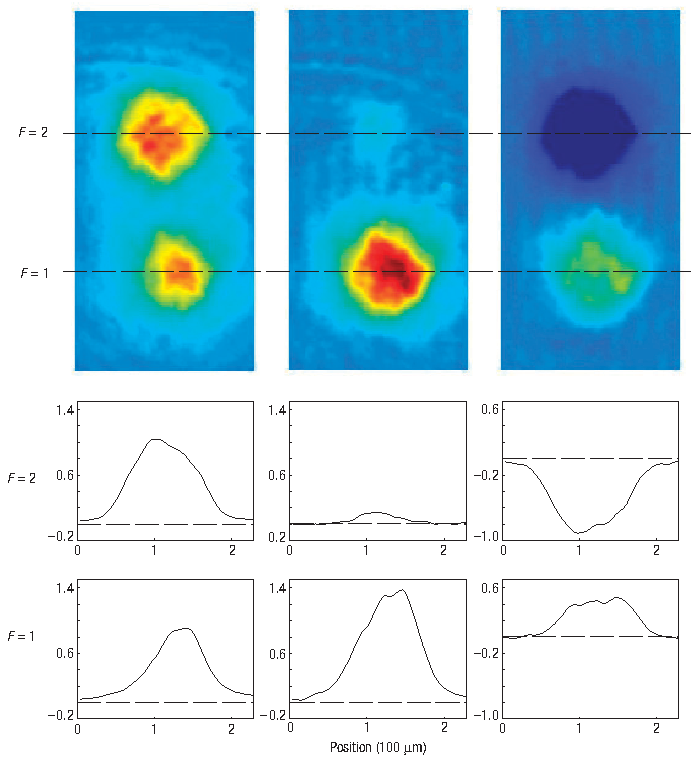
\includegraphics[width=12cm]{ExperimentalResults}
    \caption{FIXME: Caption.  Blue-detuned absorption images averaged over three identical runs of the experiment (top row); detuning of the probe laser from resonance is $\unit[7]{MHz}$.  The graphs below are horizontal cross-sections through the absorption images, showing optical depth, averaged over $\unit[50]{\micro m}$ in the vertical direction.  The tree columns correspond to: pumping off (left); pumping on (centre); difference between pumped and unpumped (right).}
    \label{OpticalPumping:ExperimentalResults}
\end{figure}

To isolate and study the pumping mechanism, the experiment was first operated without outcoupling from the laser-mode condensate.  \figureref{OpticalPumping:ExperimentalResults} demonstrates the effect \unit[200]{ms} of pumping has on the $\ket{1, -1}$ condensate; the left-hand image is taken without outcoupling from either condensate and without the pumping light.  The absorption image shows the unpumped $F=1$ laser-mode BEC (the lower cloud) with the $F=2$ source atoms above.  The curves below are horizontal cross-sections through the absorption images showing the optical depth of each atom cloud.  The central image shows the effect of \unit[200]{ms} of pumping on the laser-mode BEC.   The source is almost completely depleted and the laser-mode atom number has increased to $(7.2 \pm 0.4)\times 10^5$.  The third column shows the difference between the pumped and unpumped images. It is important to note that the profile of the laser-mode condensate after pumping has a significant Thomas-Fermi component with a small increase in the Gaussian thermal component.  The pumping efficiency, which is defined as the growth of the laser mode compared with the loss from the source, is $(35 \pm 10)\%$ for the results presented in \figureref{OpticalPumping:ExperimentalResults}.

A second experiment was also performed simultaneously pumping the laser-mode BEC and outcoupling from this condensate to demonstrate that the production of the atom laser could be operated independently of the pumping mechanism into the condensate.  In this chapter we focus on the results of the first experiment in which the pumping mechanism was studied.

\parasep

The continuous pumping experiment just described was designed to transfer $2 \hbar k$ of momentum to the falling pump atoms (by absorbing a photon of momentum $\hbar k$ going up and then emitting a photon of similar momentum directed downwards) as they are transferred to the laser-mode condensate.  However, there is a second way for the pump atoms to be momentum-resonant with the laser-mode condensate.  If the outcoupling surface for the upper condensate is towards the lower edge of the condensate the outcoupled atoms will be in close proximity to the laser-mode condensate immediately below due to the slight spatial overlap.  These recently outcoupled atoms will have almost no momentum and will be able to absorb a $\pi$-polarised photon with momentum $\hbar k$ upwards and emit a $\sigma^+$-polarised photon of similar momentum also directed upwards, decaying into the lower laser-mode condensate with no net momentum transfer.

These two different processes are examined in greater detail theoretically in \sectionref{OpticalPumping:MultimodeModel}, however we begin our theoretical analysis of the experiment and the pumping mechanism more generally with a simple single-mode model of the process illustrated in \figureref{OpticalPumping:LambdaModel}(a).


\section{Simple single-mode model}
\label{OpticalPumping:SingleModeModel}

We begin our theoretical investigation of the pumping mechanism behind the previously-described experiment by considering the simplest-possible model, a single-mode mean-field approximation to the process illustrated in \figureref{OpticalPumping:LambdaModel}(a).  The equations of motion for this model are
\begin{subequations}
    \label{OpticalPumping:SingleModeModel}
    \begin{align}
        \frac{d}{dt} c_\text{source} &= -i \Omega^* c_\text{excited} \\
        \frac{d }{dt}c_\text{excited} &= -i \Omega c_\text{source} -i g \alpha c_\text{lasing} - i \Delta c_\text{excited} - \frac{\Gamma}{2} c_\text{excited}\\
        \frac{d }{dt}c_\text{lasing} &= -i g^* \alpha^* c_\text{excited} \\
        \frac{d }{dt}\alpha &= -i g^* c_\text{lasing}^* c_\text{excited}^{\phantom{*}} - \frac{\gamma}{2} \alpha,
    \end{align} 
\end{subequations}
where $c_\text{source}$, $c_\text{lasing}$ and $c_\text{excited}$ are the amplitudes of the source $\ket{1}$, lasing $\ket{2}$ and excited $\ket{3}$ modes respectively, $\Omega$ is the complex Rabi frequency due to the pumping laser coupling the source and excited modes with detuning $\Delta$, $\alpha$ is the amplitude of the optical mode into which the excited atoms emit when decaying into the lasing mode and $g$ is the complex coupling constant for this transition.  The optical mode $\alpha$ will decay as photons propagate away from the system.  This process is modelled phenomenologically with a loss rate $\gamma$ from the optical mode $\alpha$.  The spontaneous decay of the excited state into modes other than the lasing mode occurs at a rate $\Gamma$.  It has been assumed that the pumping laser is sufficiently strong to be negligibly absorbed.  This assumption is relaxed in \sectionref{OpticalPumping:MultimodeModel}.  The evolution equations \eqref{OpticalPumping:SingleModeModel} are given in a rotating frame in which the energy difference between the source, excited and lasing modes have been appropriately removed.

In deriving \eqref{OpticalPumping:SingleModeModel} it has been assumed that atoms that undergo spontaneous decay from the excited mode will have no further impact upon the system.  In particular this means that the absorption of photons in the $\alpha$ mode by atoms in modes other than the lasing mode has been neglected.  The absorption of these photons by the lasing mode is, however, retained.  As discussed in \sectionref{OpticalPumping:PumpingMechanism} this is a valid approximation in the boson accumulation regime in which an excited atom is significantly more likely to decay into lasing mode than into any other mode.

The long-term dynamics of \eqref{OpticalPumping:SingleModeModel} will determine the usefulness of the process as a pumping mechanism.  The fast-timescale behaviour of this system can therefore be eliminated.  By far the fastest process in the system is the decay of the photons in the $\alpha$ mode as they leave the system.  The time taken for a photon to cross the width of a typical condensate ($\sim\unit[10]{\micro m}$) is $\sim\unit[10^{-13}]{s}$, giving $\gamma \sim \unit[10^{13}]{s\textsuperscript{-1}}$.  By comparison, the spontaneous decay rate of the excited mode is $\Gamma \sim \unit[10^8]{s\textsuperscript{-1}}$ for the $F'=1$ manifold of \nucl{87}{}{Rb}.  As the $\alpha$ mode reaches a quasistationary value on the fastest timescale in the system ($\gamma$), it can be adiabatically eliminated and replaced with its quasistationary limit,
\begin{align}
    \alpha & \approx -\frac{2 i g^*}{\gamma} c_\text{lasing}^* c_\text{excited}. \label{OpticalPumping:Alpha}
\end{align}

We next assume that the pump laser is driving the atoms in the weak-field regime, $\Omega \ll \max\left(\Delta, \Gamma\right)$.  In this limit, the excited mode $c_\text{excited}$ evolves on a more rapid timescale than either the source or lasing modes.  The excited mode may therefore also be adiabatically eliminated and replaced with its long-term average
\begin{align}
    c_\text{excited} &\approx \frac{-i \Omega c_\text{source}}{\frac{1}{2}\Gamma + 2 \frac{\abs{g}^2}{\gamma} N_\text{lasing} + i \Delta}, \label{OpticalPumping:CExcited}
\end{align}
where $N_\text{lasing} = \abs{c_\text{lasing}}^2$ is the number of atoms in the lasing mode.

With these two adiabatic eliminations made, the rate equations for the populations of the remaining two modes are obtained by substituting \eqref{OpticalPumping:Alpha} and \eqref{OpticalPumping:CExcited} into \eqref{OpticalPumping:SingleModeModel} giving
\begin{subequations}
    \label{OpticalPumping:SingleModeRateEquations}
    \begin{align}
        \frac{d}{dt} N_\text{source} &= - \frac{\abs{\Omega}^2 \left(\Gamma + \Gamma'\right)}{\abs{\frac{1}{2}(\Gamma + \Gamma') + i \Delta}^2} N_\text{source}\\
        \frac{d}{dt} N_\text{lasing} &= \frac{\Gamma'}{\Gamma + \Gamma'} \left( - \frac{d}{dt} N_\text{source}\right),
    \end{align}
\end{subequations}
where $\displaystyle \Gamma' = 4 \frac{\abs{g}^2}{\gamma} N_\text{lasing}$ is the rate constant with which atoms in the excited mode decay into the lasing mode.

The efficiency of the transfer of atoms in the pumping process is $\Gamma'/(\Gamma + \Gamma')$, which behaves as expected: as the occupation of the lasing mode $N_\text{lasing}$ is increased, the efficiency increases due to bosonic stimulation.  What is perhaps not expected is the behaviour of the transfer \emph{rate}.  In the limit of large detuning, $\Delta \gg \Gamma + \Gamma'$, the rate of atom transfer is
\begin{align}
    -\frac{d}{dt} N_\text{source} &\approx \frac{\abs{\Omega}^2}{\Delta^2} \left(\Gamma + \Gamma'\right) N_\text{source},
\end{align}
which increases as the lasing mode population increases (due to increasing $\Gamma'$).  In the limit of small detuning however ($\Delta \ll \Gamma + \Gamma'$) very different behaviour is obtained
\begin{align}
    -\frac{d}{dt} N_\text{source} &\approx 4 \frac{\abs{\Omega}^2}{\Gamma + \Gamma'} N_\text{source}, \label{OpticalPumping:SingleModePumpingRateZeroDetuning}
\end{align}
which \emph{decreases} as the lasing mode population increases.  This behaviour is due to the depletion of the excited state as $\Gamma'$ increases.  In the limit of small detuning, spontaneous and stimulated decay are the fastest processes reducing the occupation of the excited state, hence increasing those rates will reduce the overall population of the excited state.  In this limit as the excited state population decreases proportional to the square of these rates
\begin{align}
    N_\text{excited} &\approx 4 \frac{\abs{\Omega}^2}{(\Gamma + \Gamma')^2} N_\text{source},
\end{align}
the overall rate of atom transfer is suppressed as these processes occur on faster timescales.  In the opposite limit of large detuning, the spontaneous and stimulated decay processes are a perturbation on the Rabi-flopping process which populates the excited state.  In this limit the excited state population is independent of the spontaneous and stimulated emission rates
\begin{align}
    N_\text{excited} &\approx \frac{\abs{\Omega}^2}{\Delta^2} N_\text{source},
\end{align}
and the overall atom transfer rate into the lasing mode can be Bose-enhanced.

\parasep

The simple model developed in this section can be applied to the continuous pumping experiment described in \sectionref{OpticalPumping:ContinuousExperiment} to give a limit for the efficiency of the `$2 \hbar k$' momentum-transfer process.  In this process falling atoms outcoupled from the upper condensate reach a momentum of $2\hbar k$ vertically downwards before absorbing a pump photon of momentum $\hbar k$ from below and emitting a photon of similar momentum directed downwards to decay into the lasing mode.  If it is assumed that the intensity of the pump mode is approximately constant throughout the system, then the rate of transfer of atoms into the lasing mode cannot be faster than the rate of spontaneous emission while the source atoms are not momentum-resonant with the lasing mode\footnote{When the source atoms are not momentum-resonant with the lasing mode, it is equivalent to their being no atoms in the lasing mode.  In this case, $\Gamma'=0$ and from \eqref{OpticalPumping:SingleModePumpingRateZeroDetuning} it can be seen that the spontaneous emission rate must be greater than the transfer rate into the condensate.}.  An upper bound for the efficiency of the `$2 \hbar k$' momentum-transfer process should therefore be given by the ratio of the time for which the source atoms are momentum-resonant with the condensate ($\sim\unit[100]{\micro s}$, see \sectionref{OpticalPumping:ContinuousExperiment}) to the fall time for the atoms to that point ($\sim\unit[1]{ms}$).  As the upper bound for this process $\sim 10\%$ is lower than the observed efficiency $\sim 35\%$, either the transfer of atoms into the lasing mode must significantly reduce the intensity of the pump mode, or it must be the `$0 \hbar k$' process that operates in the continuous pumping experiment.  The argument used to obtain an upper bound for the efficiency of the `$2 \hbar k$' momentum-transfer process does not apply to the `$0 \hbar k$' momentum-transfer process in which atoms outcoupled from the upper condensate can be immediately pumped into the lower condensate.

The simple model considered in this section does not take into account the behaviour of the emitted photons in the $\alpha$ mode as they traverse the source and/or lasing modes as they leave the system.  The investigation of this and other multimode effects is the subject of the next section and will be shown to lead to modifications of the behaviour described by the simple single-mode model.

\section{Multimode model}
\label{OpticalPumping:MultimodeModel}

The multimode model we use in this chapter to describe the interaction of the BEC with light is similar to the Maxwell-Schrödinger equations \citep{Zobay:2005,Zobay:2006}, however we pursue an alternate derivation here beginning with the Hamiltonian for the system,
\begin{subequations}
    \label{OpticalPumping:AtomLightHamiltonian}
    \begin{align}
        \hat{H} &= \hat{H}_\text{atoms} + \hat{H}_\text{light} + \hat{H}_\text{atoms--light}, \\
        \begin{split}
            \hat{H}_\text{atoms} &= \sum_i \int d \vect{x}\, \hat{\Psi}_i^\dagger(\vect{x}) \left[ - \frac{\hbar^2 \nabla^2}{2 M} + V_i(\vect{x}) \right] \hat{\Psi}_i(\vect{x}) \\
            &\relphantom{=} + U \sum_{ij}\int d \vect{x}\, \hat{\Psi}_i^\dagger(\vect{x}) \hat{\Psi}_j^\dagger(\vect{x}) \hat{\Psi}_j^{\phantom{\dagger}}(\vect{x}) \hat{\Psi}_i^{\phantom{\dagger}}(\vect{x}),
        \end{split}\\
        \hat{H}_\text{light} &= \sum_\lambda \int d \vect{k}\, \hbar c \abs{\vect{k}} \hat{\Phi}_\lambda^\dagger(\vect{k}) \hat{\Phi}_\lambda(\vect{k}), \\
        \hat{H}_\text{atoms--light} &= - \int d \vect{x}\, \hat{\vect{d}}(\vect{x}) \cdot \hat{\vect{E}}(\vect{x}), \label{OpticalPumping:AtomLightCouplingHamiltonian}
    \end{align}
\end{subequations}
where $\hat{\Psi}_i(\vect{x})$ is the atomic field operator for the internal atomic state $i$, $\hat{\Phi}_\lambda(\vect{k})$ is the field operator for photons of polarisation $\lambda$, the atomic dipole operator is
\begin{align}
    \hat{\vect{d}}(\vect{x}) &= \sum_{ij}\vect{d}_{ij} \hat{\Psi}_i^\dagger(\vect{x}) \hat{\Psi}_j^{\phantom{\dagger}}(\vect{x}),
\end{align}
where $\vect{d}_{ij} = -e\left<i\middle|\vect{r}\middle|j\right> = \vect{d}^*_{ji}$ is the dipole matrix element for the atomic transition $i \leftrightarrow j$, and the electric field operator is given by
\begin{align}
    \hat{\vect{E}}(\vect{x}) &= \sum_\lambda \frac{1}{(2\pi)^{3/2}} \int d \vect{k}\, \left[\vect{u}_\lambda(\vect{k}) \left(\frac{\hbar \omega_{\vect{k}}}{2\varepsilon_0} \right)^{\frac{1}{2}} \hat{\Phi}_\lambda(\vect{k}) e^{i \vect{k} \cdot \vect{x}} + \text{h.c.}\right],
\end{align}
where $\vect{u}_\lambda(\vect{k})$ is the electric polarisation unit vector for polarisation $\lambda$.

The Hamiltonian \eqref{OpticalPumping:AtomLightHamiltonian} in principle describes the full dynamics of the system including the spontaneous decay of excited atomic levels.  From this complete description of the system we wish to obtain a simplified model with which we can investigate the behaviour of the experiment described in \sectionref{OpticalPumping:ContinuousExperiment} and the underlying pumping mechanism more generally.  

The first simplification we will make to \eqref{OpticalPumping:AtomLightHamiltonian} is to assume that all atomic and optical modes are coherent states, \emph{i.e.} the mean-field approximation.  While this approximation is justified for the condensed atomic fields (which has been discussed previously in FIXME: cross-reference) and the part of the optical field due to the pumping laser, the vacuum fluctuations responsible for spontaneous emission are necessarily neglected by any mean-field model.  The effect of spontaneous emission may be partially included by adding a decay term for the excited atomic levels, however this will necessarily neglect the effect of atoms that have undergone spontaneous emission.  While some of these atoms will decay into internal atomic states that will be dark to the optical pumping laser, others will decay into the same internal atomic level as the target condensate, however with non-zero momentum.  The effect of this treatment of spontaneous emission is discussed further in \sectionref{OpticalPumping:Discussion}\footnote{FIXME: Cross-ref to unwritten content.  Check at a later date.}.

In order to obtain a semiclassical mean-field model, we first derive the Heisenberg evolution equations,
\begin{subequations}
    \label{OpticalPumping:HeisenbergEvolution}
    \begin{align}
        i \hbar \frac{\partial}{\partial t} \hat{\Psi}_i(\vect{x}) &= \left(- \frac{\hbar^2 \nabla^2}{2 M} + V_i(\vect{x}) + U\sum_j\hat{\Psi}_j^\dagger(\vect{x})\hat{\Psi}_j^{\phantom{\dagger}}(\vect{x})\right)\hat{\Psi}_i(\vect{x}) - \sum_{j} \vect{d}_{ij} \cdot \hat{\vect{E}}(\vect{x}) \hat{\Psi}_j(\vect{x}),\\
        i \hbar \frac{\partial}{\partial t} \hat{\Phi}_\lambda(\vect{k}) &= \hbar c \abs{\vect{k}} \hat{\Phi}_\lambda(\vect{k}) - \left(\frac{\hbar \omega_{\vect{k}}}{2 \varepsilon_0}\right)^{\frac{1}{2}} \vect{u}_\lambda^*(\vect{k}) \cdot \left( \frac{1}{\left(2\pi\right)^{3/2}} \int d \vect{x}\, \hat{\vect{d}}(\vect{x}) e^{-i \vect{k} \cdot \vect{x}} \right).
    \end{align}
\end{subequations}
Applying the mean-field approximation to \eqref{OpticalPumping:HeisenbergEvolution} yields equations identical in form but without hats on the operators.

Our next approximation is to neglect the fast-rotating parts of the atom--light coupling terms in \eqref{OpticalPumping:HeisenbergEvolution}, \emph{i.e.} the rotating wave approximation (RWA).  We achieve this by first separating the real-valued electric field into positive and negative frequency terms
\begin{align}
    \vect{E}(\vect{x}) &= \vect{E}_+(\vect{x}) + \vect{E}_-(\vect{x}), \\
    \vect{E}_+(\vect{x}) &= \sum_\lambda \frac{1}{(2\pi)^{3/2}} \int d \vect{k}\, \vect{u}_\lambda(\vect{k}) \left(\frac{\hbar \omega_{\vect{k}}}{2 \varepsilon_0}\right)^{\frac{1}{2}} \Phi_\lambda(\vect{k}) e^{i \vect{k} \cdot \vect{x}},\\
    \vect{E}^{\phantom{*}}_-(\vect{x}) &= \vect{E}_+^*(\vect{x}) = \sum_\lambda \frac{1}{(2\pi)^{3/2}} \int d \vect{k}\, \vect{u}^*_\lambda(\vect{k}) \left(\frac{\hbar \omega_{\vect{k}}}{2 \varepsilon_0}\right)^{\frac{1}{2}} \Phi^*_\lambda(\vect{k}) e^{-i \vect{k} \cdot \vect{x}},
\end{align}
where $\vect{E}_+(\vect{x})$ contains the positive frequency terms rotating as $e^{-i \omega_{\vect{k}} t}$, and $\vect{E}_-(\vect{x})$ contains the negative frequency terms $e^{i \omega_{\vect{k}} t}$.  In order to clarify the application of the RWA, we must separate the atomic states $j$ into ground [hereafter denoted without a prime, $\Psi_i(\vect{x})$] and excited [denoted with a primed index, $\Psi_{i'}(\vect{x})$] states.  The RWA is equivalent to retaining only the energy-conserving terms $\hat{\vect{E}}_+^\dagger(\vect{x})\hat{\Psi}_i^\dagger(\vect{x}) \hat{\Psi}_{j'}(\vect{x})$ (and their Hermitian-conjugates) of the atom--light coupling Hamiltonian \eqref{OpticalPumping:AtomLightCouplingHamiltonian}.  

Making the rotating wave approximation, the equations of motion for the mean-field become
\begin{subequations}
    \label{OpticalPumping:MeanFieldRWAEvolution}
    \begin{align}
        \begin{split}
            i \hbar \frac{\partial}{\partial t} \Psi_i(\vect{x}) &= \left( -\frac{\hbar^2 \nabla^2}{2M} + V_i(\vect{x}) + U \sum_j \abs{\Psi_j(\vect{x})}^2\right) \Psi_i(\vect{x})\\
            &\relphantom{=} - \sum_{j'} \vect{d}_{ij'} \cdot \vect{E}_+^*(\vect{x}) \Psi_{j'}(\vect{x})
        \end{split}\\
        \begin{split}
            i \hbar \frac{\partial}{\partial t} \Psi_{i'}(\vect{x}) &= \left( -\frac{\hbar^2 \nabla^2}{2M} + V_{i'}(\vect{x}) + U \sum_j \abs{\Psi_j(\vect{x})}^2 - \frac{i\hbar \Gamma}{2}\right) \Psi_{i'}(\vect{x})\\
            &\relphantom{=} - \sum_j \vect{d}_{i'j} \cdot \vect{E}_+(\vect{x}) \Psi_j(\vect{x}) 
        \end{split}\\
        i \hbar \frac{\partial}{\partial t} \Phi_\lambda(\vect{k}) &= \hbar c \abs{\vect{k}} \Phi_\lambda(\vect{k}) - \left(\frac{\hbar \omega_{\vect{k}}}{2 \varepsilon_0}\right)^{\frac{1}{2}} \vect{u}_\lambda^*(\vect{k}) \cdot \left( \frac{1}{\left(2\pi\right)^{3/2}} \int d \vect{x}\, \sum_{ij'}\vect{d}_{ij'} \Psi^*_i(\vect{x}) \Psi_{j'}(\vect{x}) e^{-i \vect{k} \cdot \vect{x}} \right). \label{OpticalPumping:MeanFieldPhotonRWAEvolution}
    \end{align}
\end{subequations}
where the damping of the excited atoms due to spontaneous emission at a rate $\Gamma$ has been included, and the density of the excited atoms has been neglected in the $s$-wave interaction term.

Our next approximation is to recognise that most of the photon modes will be empty; the photon field will only be nonzero near a finite set of wavenumbers $\vect{q}_n$ (for corresponding polarisations $\lambda_n$).  In the case of the experiment described in \sectionref{OpticalPumping:ContinuousExperiment}, only those modes excited by the optical pumping laser or emitted as atoms undergo stimulated transitions into the target condensate will be occupied.  There will also be some small range of wavenumbers occupied around each of these due to spatial variations in the strength of these fields.  If we assume that the spatial envelope of each of these occupied modes varies on a length scale much larger than the wavelength (the slowly-varying envelope approximation), then only modes within $\delta k \ll \abs{\vect{q_n}}$ will be significantly occupied.

If the occupied photon modes $\vect{q}_n$ are sufficiently separated, the photon and electric field may be decomposed as
\begin{align}
    \Phi_\lambda(\vect{k}) &= \sum_n \delta_{\lambda, \lambda_n} \Phi_{\lambda_n,\vect{q}_n}(\vect{k}), \\
    \vect{E}_+(\vect{x}) &= \sum_n \vect{E}_{+,\vect{q}_n}(\vect{x}),
\end{align}
where $\delta_{ij}$ is the Kronecker delta.

Making an approximation, the electric field components can now be written as
\begin{align}
    \vect{E}_{+, \vect{q}_n}(\vect{x}) &= \frac{1}{(2\pi)^{3/2}} \int d \vect{k}\, \vect{u}_{\lambda_n} (\vect{k}) \left(\frac{\hbar \omega_{\vect{k}}}{2\varepsilon_0}\right)^{\frac{1}{2}} \Phi_{\lambda_n, \vect{q}_n}(\vect{k}) e^{i \vect{k}\cdot \vect{x}}\\
    &\approx \frac{1}{(2\pi)^{3/2}} \int d \vect{k}\, \vect{u}_{\lambda_n}(\vect{q}_n) \left( \frac{\hbar \omega_{\vect{q}_n}}{2\varepsilon_0}\right)^{\frac{1}{2}} \Phi_{\lambda_n, \vect{q}_n}(\vect{k}) e^{i \vect{k}\cdot \vect{x}}\\
   &= \vect{u}_{\lambda_n}(\vect{q}_n) \left( \frac{\hbar \omega_{\vect{q}_n}}{2\varepsilon_0}\right)^{\frac{1}{2}} \Phi_{\lambda_n, \vect{q}_n} (\vect{x}) \\
   &= \vect{u}_{\lambda_n}(\vect{q}_n) E_{+, \vect{q}_n}(\vect{x})
\end{align}
where $\Phi_{\lambda_n, \vect{q}_n}(\vect{x})$ is the inverse Fourier-transform of $\Phi_{\lambda_n, \vect{q}_n}(\vect{k})$, and $E_{+, \vect{q}_n}(\vect{x})$ is
\begin{align}
    E_{+, \vect{q}_n}(\vect{x}) &= \left( \frac{\hbar \omega_{\vect{q}_n}}{2 \varepsilon_0}\right)^{\frac{1}{2}} \Phi_{\lambda_n, \vect{q}_n}(\vect{x}).
\end{align}

To obtain separate dynamical equations for each of the $\Phi_{\lambda_n, \vect{q}_n}(\vect{k})$ the contribution of the atomic coupling terms of \eqref{OpticalPumping:MeanFieldPhotonRWAEvolution} to the evolution of $\Phi_\lambda(\vect{k})$ must be split amongst the evolution equations for the $\Phi_{\lambda_n, \vect{q}_n}(\vect{k})$.  In the case that each atomic transition is only energy resonant with a single optical mode $\vect{q}_n$, the splitting is obvious.  It could also be the case that two or more optical modes may be energy resonant with a single atomic transition; this case is more complicated.  If the two resonant optical modes are $\pm \vect{q}_n$ (most common case, consider Bragg reflection of a laser by a condensate), then the contribution of the atomic modes can be filtered using a projector.

The new equations become
\begin{subequations}
    \label{OpticalPumping:MeanFieldRWAEvolutionSeparatedOpticalFields}
    \begin{align}
        \begin{split}
            i \hbar \frac{\partial}{\partial t} \Psi_i(\vect{x}) &= \left( -\frac{\hbar^2 \nabla^2}{2M} + V_i(\vect{x}) + U \sum_j \abs{\Psi_j(\vect{x})}^2\right) \Psi_i(\vect{x})\\
            &\relphantom{=} - \sum_{j',n} \vect{d}_{ij'} \cdot \vect{u}^*_{\lambda_n}(\vect{q}_n) {E}_{+,\vect{q}_n}^*(\vect{x}) \Psi_{j'}(\vect{x})
        \end{split}\\
        \begin{split}
            i \hbar \frac{\partial}{\partial t} \Psi_{i'}(\vect{x}) &= \left( -\frac{\hbar^2 \nabla^2}{2M} + V_{i'}(\vect{x}) + U \sum_j \abs{\Psi_j(\vect{x})}^2 - \frac{i\hbar \Gamma}{2}\right) \Psi_{i'}(\vect{x})\\
            &\relphantom{=} - \sum_{j,n} \vect{d}_{i'j} \cdot \vect{u}_{\lambda_n}(\vect{q}_n) {E}_{+,\vect{q}_n}(\vect{x}) \Psi_{j}(\vect{x}) 
        \end{split}\\
        \begin{split}
            i \hbar \frac{\partial}{\partial t} \Phi_{\lambda_n, \vect{q}_n}(\vect{k}) &= \hbar c \abs{\vect{k}} \Phi_{\lambda_n,\vect{q}_n}(\vect{k}) \\
            &\relphantom{=} - \left(\frac{\hbar \omega_{\vect{q}_n}}{2 \varepsilon_0}\right)^{\frac{1}{2}} \vect{u}_{\lambda_n}^*(\vect{q}_n) \cdot \left( \frac{1}{\left(2\pi\right)^{3/2}} \int d \vect{x}\, \sum_{\{i,j'\}\in T_n}\vect{d}_{ij'} \Psi^*_i(\vect{x}) \Psi_{j'}(\vect{x}) e^{-i \vect{k} \cdot \vect{x}} \right).
        \end{split}
    \end{align}
\end{subequations}
where we have made a couple of approximations in the last equation similar to those made earlier. Also, the above equation for $\Phi_{\lambda_n, \vect{q}_n}$ may only be nonzero for $\vect{q}_n \cdot \vect{k} > 0$
While it may seem that we have unnecessarily complicated the problem by separating one equation (two really) for the optical field into many for each significantly occupied mode, this complication will enable the use of significant simplifications later.

Perhaps we don't need the step function above, we could simply say that the $\Phi_{\lambda, \vect{q}_n}(\vect{k})$ may only be non-zero for $\vect{q}_n \cdot \vect{k} > 0$.  Perhaps a simpler method.

We should now be able to do an inverse Fourier transform. We can once we approximate $\abs{\vect{k}} \approx \unitvec{q}_n \cdot \vect{k}$ (where we use the notation $\unitvec{x}$ for the unit vector in the direction of \vect{x} to avoid confusion with the use of hats to denote operators),
\begin{align}
    \abs{\vect{k}} &= \abs{\vect{q}_n + \delta \vect{k}}\\
    &\approx \sqrt{\abs{\vect{q}_n}^2 + 2 \vect{q}_n \cdot \delta \vect{k}} = \abs{\vect{q}_n} \sqrt{1 + \frac{2 \vect{q}_n \cdot \delta \vect{k}}{\abs{\vect{q}_n}^2}}\\
    &\approx \abs{\vect{q}_n} + \unitvec{q}_n \cdot \delta \vect{k} = \abs{\vect{q}_n} + \unitvec{q}_n \cdot \left(\vect{k} - \vect{q}_n\right)\\
    &= \unitvec{q}_n \cdot \vect{k}
\end{align}
Then we obtain
\begin{align}
    i \hbar \frac{\partial}{\partial t} \Phi_{\lambda_n, \vect{q}_n}(\vect{x}) &= -i \hbar c \unitvec{q}_n \cdot \nabla \Phi_{\lambda_n, \vect{q}_n}(\vect{x}) - \left(\frac{\hbar \omega_{\vect{q}_n}}{2\varepsilon_0}\right)^{\frac{1}{2}} \vect{u}_{\lambda_n}^*(\vect{q}_n) \cdot \sum_{\{i,j'\} \in T_n} \vect{d}_{ij'} \Psi^*_i(\vect{x}) \Psi_{j'}(\vect{x})
\end{align}
Hooray.  We have made an approximation in here because we haven't correctly projected the atomic source term in the above equation.  However, the contributions will be $2 \vect{q}_n$ out of resonance, and so will average to zero over half a wavelength. Note that the above equation without the source term is the transport equation in the direction of ${\vect{q}_n}$ with speed $c$.  Next we turn it into a propagation equation for the electric field ${E}_{+,\vect{q}_n}$,
\begin{align}
    \frac{1}{c} \frac{\partial}{\partial t} E_{+, \vect{q}_n} (\vect{x}) &= - \unitvec{q}_n \cdot \nabla E_{+, \vect{q}_n}(\vect{x}) + i \frac{\hbar \abs{\vect{q}_n}}{2 \varepsilon_0} \vect{u}^*_{\lambda_n}(\vect{q}_n) \cdot \sum_{\{i,j'\}\in T_n} \frac{\vect{d}_{ij'}}{\hbar} \Psi^*_i(\vect{x}) \Psi_{j'}(\vect{x})
\end{align}

Next we need to move into appropriate rotating frames for all states.  That means including possible detunings. For the excited states, that's well-defined.  What about for the lower states too?  What is required in order to be able to go into these appropriate rotating frames is that all photons coupling to a given excited state all couple to essentially the same detuning.  This is guaranteed in our system because only one set of photons are supplied to the system.  The others are generated spontaneously.  The other way to go into an appropriate rotating frame is to define all detunings relative to an original level (but we still need consistency on all photons coupling a given level).  How does all of this mix with RF outcoupling and the associated detunings?

Rotate as $\Psi_{i} = \widetilde{\Psi}_i e^{-i (\omega_i - \Delta_i)t}$, $\Psi_{i'} = \widetilde{\Psi}_{i'} e^{-i (\omega_{i'} - \Delta_{i'})t}$, $E_{+,\vect{q}_n} = \widetilde{E}_{+, \vect{q}_n} e^{-i \omega_{\vect{q}_n}t}$. Spatial phase rotation for the electric fields? --- No.

\begin{subequations}
    \begin{align}
        \begin{split}
            i \hbar \frac{\partial}{\partial t} \widetilde{\Psi}_i(\vect{x}) &= \left( -\frac{\hbar^2 \nabla^2}{2M} + V_i(\vect{x}) + U \sum_j \abs{\widetilde{\Psi}_j(\vect{x})}^2 - \hbar \omega_{i} + \hbar \Delta_i \right) \widetilde{\Psi}_i(\vect{x})\\
            &\relphantom{=} - \sum_{j',n} \vect{d}_{ij'} \cdot \vect{u}^*_{\lambda_n}(\vect{q}_n) \widetilde{E}_{+,\vect{q}_n}^*(\vect{x}) \widetilde{\Psi}_{j'}(\vect{x}) e^{-i (\omega_{j'} - \Delta_{j'} - (\omega_i - \Delta_i) - \omega_{\vect{q}_n})t}
        \end{split}\\
        \begin{split}
            i \hbar \frac{\partial}{\partial t} \widetilde{\Psi}_{i'}(\vect{x}) &= \left( -\frac{\hbar^2 \nabla^2}{2M} + V_{i'}(\vect{x}) + U \sum_j \abs{\widetilde{\Psi}_j(\vect{x})}^2 - \frac{i\hbar \Gamma}{2} - \hbar \omega_{i'} + \hbar \Delta_{i'}\right) \widetilde{\Psi}_{i'}(\vect{x})\\
            &\relphantom{=} - \sum_{j,n} \vect{d}_{i'j} \cdot \vect{u}_{\lambda_n}(\vect{q}_n) \widetilde{E}_{+,\vect{q}_n}(\vect{x}) \widetilde{\Psi}_{j}(\vect{x})  e^{-i (\omega_{j} - \Delta_j - (\omega_{i'} - \Delta_{i'}) + \omega_{\vect{q}_n})t}
        \end{split}\\
        \begin{split}
          \frac{1}{c} \frac{\partial}{\partial t} \widetilde{E}_{+, \vect{q}_n} (\vect{x}) &= - \frac{\vect{q}_n}{\abs{\vect{q}_n}} \cdot \nabla \widetilde{E}_{+, \vect{q}_n}(\vect{x}) + i \abs{\vect{q}_n} \widetilde{E}_{+, \vect{q}_n}(\vect{x})\\
          &\relphantom{=} + i \frac{\hbar \abs{\vect{q}_n}}{2 \varepsilon_0} \vect{u}^*_{\lambda_n}(\vect{q}_n) \cdot \sum_{\{i,j'\}\in T_n} \frac{\vect{d}_{ij'}}{\hbar} \widetilde{\Psi}^*_i(\vect{x}) \widetilde{\Psi}_{j'}(\vect{x}) e^{-i (\omega_{j'} - \Delta_{j'} -\omega_i + \Delta_i - \omega_{\vect{q}_n})t}
        \end{split}
    \end{align}
\end{subequations}

$\omega_{j'} - \Delta_{j'} - (\omega_i - \Delta_i) = \omega_{\vect{q}_n} \forall \; \{i, j'\} \in T_n$? 

The frame transformation we wish to make is
\begin{align}
  \vect{x}' &= \vect{x} \\
  t' &= t - \frac{1}{c} \unitvec{q}_n \cdot \vect{x}
\end{align}
This means that
\begin{align}
  \frac{\partial}{\partial t} &= \frac{\partial }{\partial t'}\\
  \nabla_{\vect{x}} &= \left(\nabla_{\vect{x}} t'\right) \frac{\partial }{\partial t'} + \nabla_{\vect{x}'}\\
  &= - \frac{1}{c} \unitvec{q}_n\frac{\partial}{\partial t'} + \nabla_{\vect{x}'}
\end{align}
This gives our equation for $\widetilde{E}_{+, \vect{q}_n}$ as
\begin{align}
  \begin{split}
    \frac{1}{c} \frac{\partial}{\partial t'} \widetilde{E}_{+, \vect{q}_n} (\vect{x}', t') &= - \unitvec{q}_n \cdot \left(- \frac{1}{c} \unitvec{q}_n \frac{\partial}{\partial t'} + \nabla_{\vect{x}'} \right) \widetilde{E}_{+, \vect{q}_n}(\vect{x}', t') + i \abs{\vect{q}_n} \widetilde{E}_{+, \vect{q}_n}(\vect{x}', t')\\
    &\relphantom{=} + i \frac{\hbar \abs{\vect{q}_n}}{2 \varepsilon_0} \vect{u}^*_{\lambda_n}(\vect{q}_n) \cdot \sum_{\{i,j'\}\in T_n} \frac{\vect{d}_{ij'}}{\hbar} \widetilde{\Psi}^*_i\left[\vect{x}', t(\vect{x}', t')\right] \widetilde{\Psi}_{j'}\left(\vect{x}', t(\vect{x}', t')\right)
  \end{split}
\end{align}
which simplifies to
\begin{align}
  \begin{split}
    \frac{1}{c} \frac{\partial}{\partial t'} \widetilde{E}_{+, \vect{q}_n} (\vect{x}', t') &= - \unitvec{q}_n \cdot \left(- \frac{1}{c} \unitvec{q}_n \frac{\partial}{\partial t'} + \nabla_{\vect{x}'} \right) \widetilde{E}_{+, \vect{q}_n}(\vect{x}', t') + i \abs{\vect{q}_n} \widetilde{E}_{+, \vect{q}_n}(\vect{x}', t')\\
    &\relphantom{=} + i \frac{\hbar \abs{\vect{q}_n}}{2 \varepsilon_0} \vect{u}^*_{\lambda_n}(\vect{q}_n) \cdot \sum_{\{i,j'\}\in T_n} \frac{\vect{d}_{ij'}}{\hbar} \widetilde{\Psi}^*_i\left[\vect{x}', t(\vect{x}', t')\right] \widetilde{\Psi}_{j'}\left(\vect{x}', t(\vect{x}', t')\right)
  \end{split}
\end{align}


Then we do a frame transform for each $\vect{q}_n$.  Really only works for one... how can we justify this for each and every direction (in our case, just two).

I can't say anything about ${\pi\slashed{\pi}}\bar{\pi}$ We need to be able to separate the optical field equation of motion.  I suspect that means that we need to assign $\left(i, j\right)$ pairs to $\vect{q}_i$ values.  There is also a question about sign... i.e. what is the distinction between $\pm \vect{q}_i$?



Steps remaining:
\begin{itemize}
    \item Neglect retardation effects
    \item 1D
    \item Polarisation?? --- Not quite sure yet how to treat this.
    \item Adiabatic elimination
\end{itemize}

Hooray.  Next we separate the electric field and apply the SVE approximation. So we then have a bunch of $\Phi_{\vect{k}_0,\lambda}(\vect{k})$'s, each centred around a $\vect{k}_0$. At this point we approximate the $\omega_{\vect{k}}\approx \omega_{\vect{k}_0}$ also the time and phase variation must be removed at this point, requiring the removal of appropriate terms from the atomic fields.  Then we reduce to 1D, allowing us to inverse Fourier transform the $\Phi_{\vect{k}_0, \lambda}(\vect{k})$.  Finally we neglect retardation effects to remove the time derivatives.  Then we have our 1D multimode Maxwell-Schrödinger equations.  Oh, and we need to re-introduce loss.  Then we can adiabatically eliminate the excited states to obtain our model of the system.  As if that is not complicated.

This spontaneous emission process can be approximated by including the decay of the excited levels in a 

This spontaneous emission process is well-described


This spontaneous emission process is well-described by the 



To approximate this system we will treat the electric field as having a finite number of highly-occupied contributions with the remaining electric field modes causing the spontaneous decay of all excited atomic levels.  The spontaneous decay will be introduced in the usual way at a later stage; we continue focusing on the photon modes.



The multimode model we use in this chapter to describe the interaction of the BEC with the optical fields is similar to the Maxwell-Schrödinger equations \citep{Zobay:2005,Zobay:2006}, however we pursue a different derivation here beginning with / starting from the Hamiltonian for the system.


from consideration o the Hamiltonian describing the atoms, light and their interaction.  Perhaps a different lead-in.

The multimode model describing the interaction of atoms and light 


A multimode model for the pumping mechanism considered in this chapter can be obtained by consideration of the Hamiltonian describing the atoms, light and their interaction.




A multimode model for the pumping mechanism considered in this chapter can be obtained by consideration of the Hamiltonian describing the system dynamics.  



Here we need to describe the general system of equations, the Maxwell-Schrödinger equations.  Describe how they are solved, and then apply them to various systems. Screw the usual method, let's go from the Hamiltonian:

\begin{align}
    \begin{split}
        \hat{H} &= \sum_j \int d \vect{x}\, \hat{\Psi}_j^\dagger(\vect{x}) \left[ - \frac{\hbar^2 \nabla^2}{2 M} + V_j(\vect{x}) \right] \hat{\Psi}_j(\vect{x}) + \sum_\lambda \int d \vect{k}\, \hbar c \abs{\vect{k}} \hat{\Phi}_\lambda^\dagger(\vect{k}) \hat{\Phi}_\lambda(\vect{k}) \\
        &\relphantom{=}- \int d \vect{x}\, \hat{\vect{d}}(\vect{x}) \cdot \hat{\vect{E}}(\vect{x})
    \end{split}
\end{align}

\begin{align}
    \hat{\vect{E}}(\vect{x}) &= \sum_\lambda \frac{1}{(2\pi)^{3/2}} \int d \vect{k}\, \left[\vect{u}_\lambda(\vect{k}) \left(\frac{\hbar \omega_{\vect{k}}}{2\varepsilon_0} \right)^{\frac{1}{2}} \hat{\Phi}_\lambda(\vect{k}) e^{i \vect{k} \cdot \vect{x}} + \text{h.c.}\right],
\end{align}
where $\vect{u}_\lambda(\vect{k})$ is a unit vector for the corresponding polarisation, $\hat{\Phi}_\lambda(\vect{k})$ is the photon annihilation operator in momentum space for the $\lambda$ polarisation, $\lambda = \pm 1$.

It is important to note that the above Hamiltonian essentially retains spontaneous emission.

We can approximate the above expression in the slowly-varying envelope (SVE) approximation
\begin{align}
    \hat{\vect{E}}(\vect{x}) &\approx \sum_\lambda \frac{1}{(2\pi)^{3/2}} \left(\frac{\hbar k_\gamma c}{2\varepsilon_0} \right)^{\frac{1}{2}} \int d \vect{k}\, \left[\vect{u}_\lambda \hat{\Phi}_\lambda(\vect{k}) e^{i \vect{k} \cdot \vect{x}} + \text{h.c.}\right],
\end{align}

\subsection{Two overlapping condensates model}

\subsection{Atom laser model}

\subsection{3-level model}

\subsection{5-level model}
The 1D model is based on the Maxwell-Schrödinger equations.  One of the technical difficulties is the fact that we must be able to solve in the case that light is travelling in opposite directions simultaneously.  It is not an issue analytically, the equations are well-defined.  The trouble is solving the system self-consistently.  The equations as posed are stiff and are best treated by implicit algorithms, but the best we have are half-arsed semi-implicit algorithms. Better yet would be to use a finite-element method and treat the cross-propagation properly, but I'm lazy.  The other issue is that the frequency of the light is usually known \emph{a priori}.  That is not the case for at least one of the modes in this system.  We therefore need to use some fancy tricks in order to get around that issue.  However, any detunings should not be too large.

Apart from the Maxwell part of the system of equations, everything else is fairly standard.  Except of course for the 1D reduction itself.  We'll call it a `central-line' approximation.

Somewhere in here we need to mention the adiabatic elimination and what kinds of terms it gives rise to.  And in what limit the approximation is valid (even close to resonance).

We need to talk about the other assumptions made in the model.  The assumption that spontaneous emission is negligible.  There is a question about how the 1D approximation affects the Franck-Condon factor, and the relationship between that and spontaneous emission.

Now is a good time to consider $0 \hbar k$ vs $2 \hbar k$ and resonant vs detuned in a simplified model in which things can be controlled (two overlapping modes in the same trap and where $k \rightarrow 0$). The important difference being the \emph{geometry}.

\subsection{3-level model}

This is a simplified model that contains only a small number of levels so that it is easier to keep track of what is going on.  We assume that we can outcouple directly from the $F=2$, $m_F=2$ trapped condensate to the $F=2$, $m_F=0$ state. This isn't realistic, but it is useful to simplify the whole process.  I believe the excited $F'$ manifold was also reduced.  With this simplified model we can investigate resonance vs detuned.  I seem to recall some crazy interesting physics where we had atom transfer back to the \emph{source} condensate in the $0 \hbar k$ configuration in the detuned case.  I believe it was all about phase differences and stuff.  If you look at the equations from the zero-dimensional model, the direction of transfer depends on the phase of a couple of terms, so it can go either way.  For the resonant case, the atoms were definitely transferred to the \emph{target} condensate, as desired.  Also, try as we might, it was not possible to get the $2 \hbar k$ resonance working efficiently.  Too much loss on the way.  Though I don't remember what happened in the detuned $2 \hbar k$ case.

This simplified 1D model contains all of the important physics related to the pumping process.  The delivery of atoms to the target condensate is simplified, and some of the optical transitions are removed.  This model is partly to validate the simple zero-dimensional model including some multimode dynamics, and also to try to get some basic agreement with the experiment before moving on to a more complete description in a later section.

\subsubsection{Comparison with experiment}

We consider both the $0\hbar k$ and the $2\hbar k$ resonance and find that we are able to get reasonable agreement with the experiment in the $0\hbar k$ limit, although it was incredibly fiddly to maximise the transfer.  The $2\hbar k$ resonance was dominated by loss of atoms as they travelled between the source and target condensates.  Although it must be stated that the experimentalists had a good idea of their detunings from rf spectroscopy.  The detunings did indicate that the required conditions for the $0 \hbar k$ resonance were not present.  They were however appropriate for the $2 \hbar k$ resonance, which was the one originally hoped for.  I can't remember, but I wanted to reproduce the experimental rf-spectroscopy data theoretically for some reason.

Anyway, things look great. So why don't we add more realism and see what we get? Maybe we can get even better agreement!

\subsection{5-level model}

The 5-level model is like the 3-level model, but including the full $F=2$ manifold.  Also, the full $F'=1$, $F'=2$ and $F'=3$ excited state manifolds are included before adiabatic elimination.  This model is designed to illustrate the full physics of the situation.  

\subsubsection{Comparison with experiment}

The theory in this case is completely defeated by the crazy mode shape of the $F=2$, $m_F=1$ level.  As this mode is trapped, it oscillates about the lower condensate.  If the intensity of the light is too low, these atoms block the pumping light from even reaching the target condensate and the $F=2$, $m_F=0$ atoms.  If the intensity of the light is too high, the atoms undergo spontaneous emission before they even reach the lower condensate, and you don't get any $F=2$, $m_F=0$ atoms.  If you try for something in the middle, the Franck-Condon factor between the $F=2$, $m_F=0$ atoms and the condensate is very small due to the crazy mode shape of the $F=2$, $m_F=1$ atoms from which the $F=2$, $m_F=0$ atoms are outcoupled.

In short, the 5-level model shows no pumping at all. But not because of something fundamental with the atom transfer process, but rather due to boring technical details about providing the atoms in the appropriate state and mode.  Besides, 1D models are very poor approximations to 5-level systems on timescales beyond the time for the $F=2$, $m_F=1$ atoms to reach the centre of that trap as the atoms will focus at the origin in the tight trapping dimension significantly increasing the density there over what would be seen in a purely 1D model.

\subsection{The pulsed pumping experiment}

The pulsed pumping experiment had the same basic set up as the continuous experiment, but instead a pulse of atoms (the \emph{transfer pulse}) was outcoupled from the upper condensate.  As this pulse was outcoupled over $\unit[100]{\micro s}$ (or whatever time it was) the issue of detuning essentially doesn't arise.  The Fourier width of the outcoupling pulse is large enough to essentially outcouple a copy of the condensate into the different Zeeman levels.  This transfer pulse was allowed to fall a variable delay time before pulsing on the same pumping light used in the continuous experiment.  The transfer pulse was finally allowed to fall further before imaging to determine the number of atoms remaining in the transfer pulse.  Due to the vastly different densities of the condensate and the transfer pulse, it is impossible to simultaneously measure the size of each.  Moreover, as the transfer pulse is significantly smaller than the target condensate, it was impossible to determine the number of transferred atoms to the target condensate.

\subsubsection{Theory / Experiment comparison}

We have good agreement with the loss of atoms out of the transfer pulse, which suggests that the $2 \hbar k$ resonance is workable, although it must be realised that operating a pulsed experiment is fundamentally different to the operation of the continuous experiment.  One model for the operation of the continuous experiment suggests that a process like STIRAP is occurring in the spatial domain instead of the usual temporal domain.  By operating the experiment in the pulsed regime, we are able to cause this process to occur in the temporal domain again, allowing access to the $2 \hbar k$ resonance.  Regardless, there are some questions that remain unanswered.  While we have good agreement on the transfer of atoms \emph{out} of the pulse, the experiment has no information about the transfer of atoms \emph{into} the condensate.  For this question, we can only rely on the theory.  In this case, the theory suggests that there should be a significant number of photons emitted spontaneously within the lower condensate.  A single one of these photons should cause significant (observable) heating of the lower condensate.  The issue is that no such heating is observed.  We are left scratching our heads on this issue (see next section).

\section{Discussion / Outlook}
\label{OpticalPumping:Discussion}

This is where we say that we have reasonable evidence to say that we know what is going on in the transfer of atoms to the lower condensate, but a pretty poor explanation for what happens afterwards.  It is precisely this latter process that was thought to prevent optical pumping of condensates, and so the fact that the expected heating has not been observed is of great interest.  We can speculate wildly as to the origin of this absent heating, including BAR and quantum-mechanical collective effects due to the coherence of the atom laser.  Fundamentally, it seems to me that the notion of spontaneous emission is broken when the emission is occurring in the centre of a BEC.  On the edge, it probably mostly works.  In the centre, I'm not entirely convinced.

\section{Conclusion}

The conclusion I have been thinking of at the moment is along the following lines.  There have been three parts to the optical pumping process: (i) the delivery of atoms in an appropriate state to the condensate being pumped; (ii) the transfer of those atoms to the condensate being pumped; and (iii) the behaviour of the emitted photons within the pumped condensate.  This present chapter has aimed to understand part (ii) of this process.  Ideally we would also like to understand (iii) as it appears that there is some very interesting physics occurring in this part of the process, however we have fallen short of this goal.  By contrast process (i) is a technical detail of getting atoms to the lower condensate with an appropriate mode.  There are several methods that could be used for this process, and there are a number of arguments why the models used in this chapter are unsuitable for fully describing process (i).  Technical details are of course important, but not of fundamental importance.  And it has been the fundamentally important processes that we have aimed to investigate in the present chapter.


\chapter{Evaporation-induced pumping of an atom laser}
\label{KineticTheory}
\graphicspath{{Figures/KineticTheory/}{Figures/Common/}}

FIXME: Consider stating that this code is derived from the code used in previous quantum kinetic theory papers, and has therefore been validated both against independently created codes and against experiment (in a different situation).

The pumping process of an atom laser --- just like that of an optical laser --- is a necessarily irreversible process. This irreversibility enters through the coupling of the lasing mode to a much larger system (the reservoir).  For the optical laser this is comprised of the (almost) empty modes of the optical field that the atoms decay into after emitting a photon into the lasing mode (see \sectionref{Introduction:ThePumpingMechanism}).  In the case of the atom laser, there are two possible choices for the reservoir providing the irreversibility: empty modes of an optical field, or empty modes of an atomic field.  The former case was considered in the previous chapter; the latter is the subject of this chapter. 

% The results presented in this chapter have been submitted for publication\footnote{FIXME: Not yet true, but it is intended that this be the case.}.  
The results and analysis presented in \sectionref{KineticTheory:Results} of this chapter was my own work.  The model presented in \sectionref{KineticTheory:Model} is based on prior work~\citep{Davis:2000vn,Bijlsma:2000}.  The derivation of the three-body loss term in \sectionref{MethodsAppendix:QKT3BodyLoss} and the code the results in this chapter are based on are the work of \emph{Matthew Davis}.

\section{Introduction}

Continuous pumping of an atom laser is a key tool for producing superior atomic sources. Besides the obvious benefit of higher flux, it also promises improved modal stability \citep{Haine:2002kp,Haine:2003fs} and linewidth \citep{Johnsson:2007}, much as it does for the optical laser.

There are two essential steps towards the continuous pumping of an atom laser. The first is a delivery system for filling an atomic reservoir with ultracold atoms. The second is a process that causes at least some of those atoms to make an irreversible, atom-stimulated transition into the BEC.

Continuous delivery of ultracold atoms has been demonstrated in a number of experiments \citep{Schmid:2006,Lahaye:2004,Greiner:2001,Greiner:2007,Streed:2006,Muller:2007}, and is an important component of thermal atomic interferometry experiments.  The atom-stimulated transitions into the condensate can be made irreversible by coupling to a reservoir. In this chapter we consider the case in which the reservoir is comprised of empty modes of the atomic field accessible via evaporation.

Sequential reloading of a target BEC was achieved using optical tweezers~\citep{Chikkatur:2002qa}, where a series of source condensates were added adiabatically by manipulating the trapping potentials, and excitations were subsequently removed by continuous evaporation. This milestone experiment maintained the condensate fraction, and therefore the potential flux of a potential atom laser. An atom laser produced from such an experiment would, however, not possess the desired narrow linewidth as the source condensates used were of a similar size to or larger than the condensate being replenished causing significant scattering into modes other than the target condensate. To produce an atom laser with a narrow linewidth it would be necessary for the atomic source to negligibly disrupt the target condensate.  While this could be achieved by merging the target condensate with significantly smaller condensates more frequently, it is technically very challenging to develop high flux sources of Bose-condensed atoms compared to sources at higher temperature, which have a higher average flux. In this chapter it is shown that a similar experiment using an ultra-cold \emph{thermal} source ought to be able to pump the target BEC and maintain a significant BEC population using a phase-preserving Bose-enhanced process.

%This method has the advantage that it can be performed without the presence of resonant light, but the obvious disadvantage that it relies on the system approaching thermal equilibrium, and will therefore be reversed by the addition of atoms above the condensate temperature. In this chapter it is demonstrated that a driven system undergoing evaporative cooling can produce a high-flux, phase-stable atom laser for a range of experimental parameters.

% FIXME: Something about the fact that one of the distinguishing aspects of this work is the inclusion of three-body loss, as it has been omitted in previous models. While that may be adequate for treatments of the process of condensation, it is inadequate for any treatment of the creation of a pumped atom laser (as will be later argued).

\section{Scheme}
\label{KineticTheory:Scheme}

\begin{figure}
    \centering
        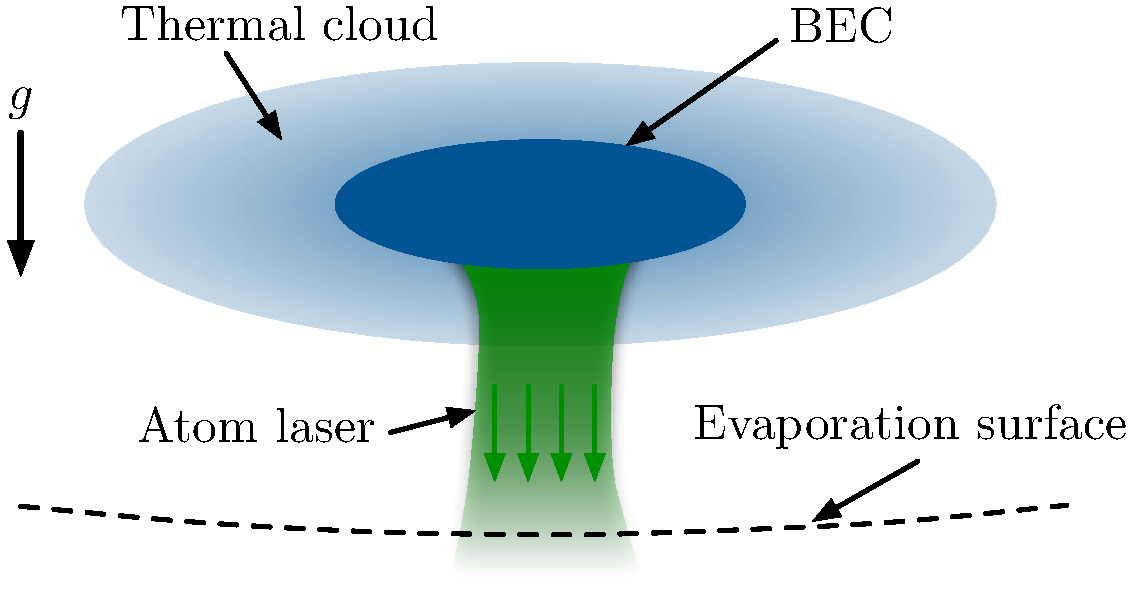
\includegraphics[width=10cm]{QKTScheme}
    \caption{Schematic of the experimental setup.}
    \label{KineticTheory:QKTScheme}
\end{figure}

The proposed scheme for a pumped atom laser is illustrated in \figureref{KineticTheory:QKTScheme} and is very similar to the processes used to evaporate a thermal cloud to condensation in a magnetic trap and produce a (quasi-continuous) atom laser. The additional element in this scheme is a process for replenishing the cloud of thermal atoms in the trap.  

In this scheme the gain process for the condensate is the same Bose-enhanced scattering between thermal atoms and the condensate that drives condensate growth when evaporating to produce condensate~\citep{Gardiner:1997kx,Davis:2000vn,Bijlsma:2000}.  This process becomes irreversible when one of the scattered atoms has enough energy to cross the evaporation surface and be removed from the thermal cloud.  The loss of atoms from the thermal cloud is balanced by a replenishment process that couples the thermal cloud to a source of atoms at finite temperature.

The atom laser beam itself is produced by outcoupling from the condensate.  To minimise direct outcoupling from the thermal cloud, this outcoupling process should be a large momentum-transfer Raman process to limit the range of momenta of thermal particles that will be outcoupled.  Outcoupling of thermal atoms can be reduced further by focussing the Raman lasers to only intersect in the immediate vicinity of the condensate.

A dynamic equilibrium will be reached when the rate of atom loss from the condensate due to outcoupling balances the rate of atoms gained due to scattering with the thermal cloud.  If the evaporative surface is tuned so that atoms of energy $\varepsilon_\text{cut}$ and higher are rapidly and continually removed from the trap, then all collisions that give atoms energy greater than $\varepsilon_\text{cut}$ will become irreversible. As $\varepsilon_\text{cut}$ is lowered, a larger fraction of the scattering processes that leave atoms in the condensate mode will become irreversible. This suggests that there must be some value of $\varepsilon_\text{cut}$ for which the condensate experiences net gain. What is not clear is whether the net gain can proceed efficiently, i.e.\ on a timescale much shorter than other losses from the condensate.  Lowering $\varepsilon_\text{cut}$ also reduces the total number of thermal atoms present. In the limit that $\varepsilon_\text{cut}$ reaches the condensate energy, there will be no background gas at all, and the condensate cannot experience net gain.  We therefore expect that for a given set of parameters, there will be an optimal value for $\varepsilon_\text{cut}$ that maximises the net gain, which may or may not be positive. In order to examine this issue, quantum kinetic theory (QKT)~\citep{Gardiner:1997tz,Jaksch:1997ug,Gardiner:1998wx,Jaksch:1998sj,Gardiner:2000ug,Lee:2000vs,Davis:2000vn} has been employed, which has been effective in describing the growth of condensates~\citep{Davis:2000vn}.


\section{Model}
\label{KineticTheory:Model}

\begin{figure}
    \centering
        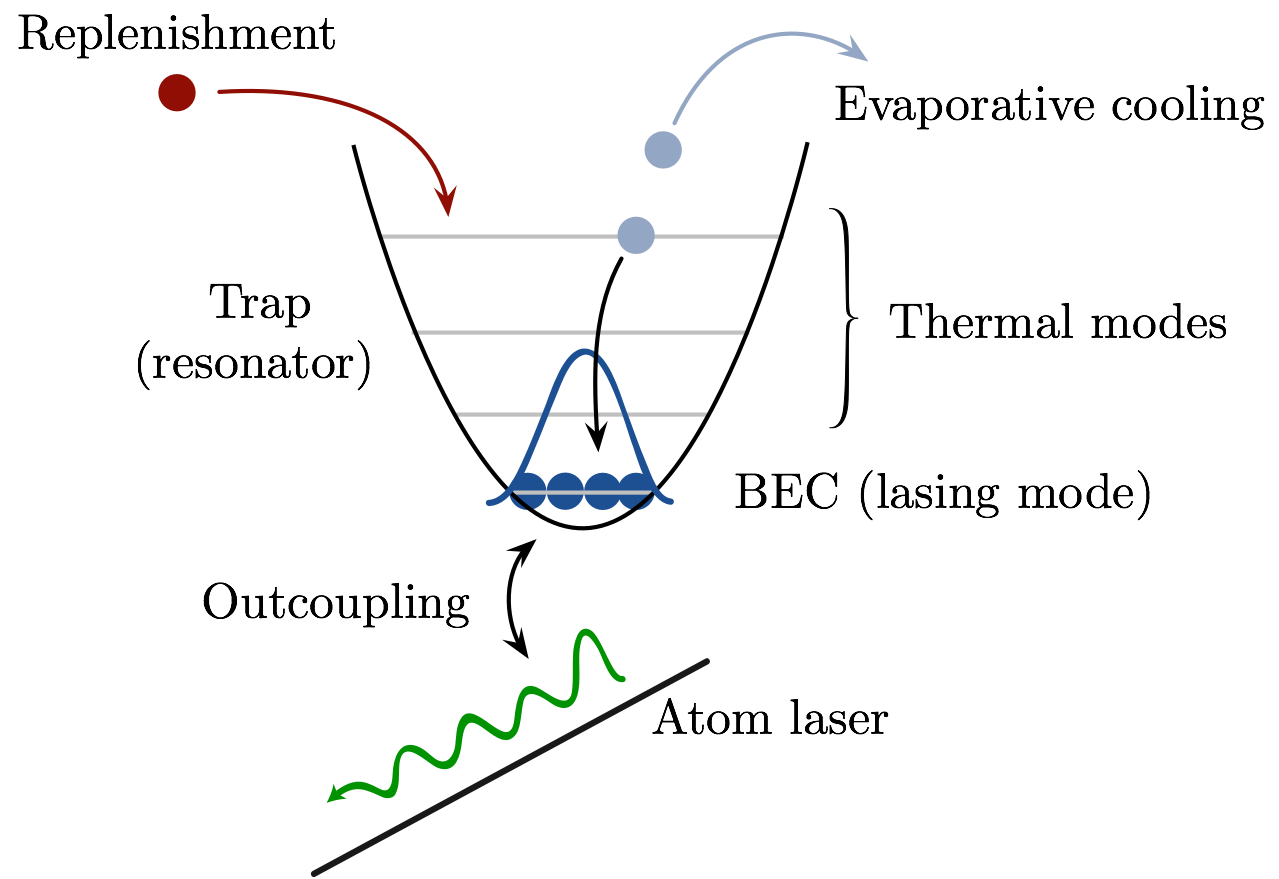
\includegraphics[width=10cm]{QKTModel2}
    \caption{Schematic of the theoretical model.}
    \label{KineticTheory:QKTModel}
\end{figure}

The theoretical model described in this section is an extension of the kinetic model of~\citet{Bijlsma:2000}, which was successfully used to study condensate growth in an experiment in which a cloud of thermal atoms just above condensation temperature were shock-cooled below transition~\citep{Miesner:1998}.  After shock-cooling, the atoms were left to equilibrate, with condensate formation being driven by the same collisional processes that would drive condensate growth in the proposed pumped atom laser experiment described in the previous section.  To fully describe this proposed experiment, the kinetic model of~\citeauthor{Bijlsma:2000} must be modified to include the effects of the replenishment and outcoupling processes illustrated in \figureref{KineticTheory:QKTScheme}. 

Another important process that must be included in the model is three-body recombination, which is the dominant loss process in typical BEC experiments~\citep{Burt:1997fk,Soding:1999}. Without the inclusion of this process, for given replenishment and outcoupling rates, the largest condensate would be formed in the absence of evaporation as outcoupling from the condensate would be the only loss process in the system. In fact, this condensate number would be independent of the temperature of the replenishment source, depending only on the flux of atoms delivered to the system and the outcoupling rate from the condensate. This unphysical result is because in the absence of a density-dependent loss process, simply increasing the density is a feasible method of approaching degeneracy. It would be possible to reach condensation with room-temperature atoms in a harmonic trap simply by confining enough atoms! To avoid such unphysical results, the effect of three-body loss as the dominant density-dependent loss process must be included in the model.

\parasep

The starting point of the kinetic model presented here is to treat separately the thermal and condensed components of the system in \figureref{KineticTheory:QKTScheme}.

The condensed component is assumed to be a quantum fluid obeying a Gross-Pitaevskii-type equation, however we make a further approximation and assume that the condensate is sufficiently occupied that it has a Thomas-Fermi profile.  The condensate dynamics are then fully described by the number of condensed atoms $N_0(t)$.

The thermal cloud is assumed to be well described within the Hartree-Fock approximation~\citep[Chapter 8]{PethickSmith} as comprised of particle-like excitations moving in the effective potential of the harmonic trap plus condensate mean field.  To reduce the dimensionality of the full phase-space distribution function for the thermal cloud $f(\vect{r}, \vect{p}, t)$, it is assumed that the system is ergodic, i.e.\  that all points in the phase space having the same energy are equally probable.  Under this approximation, the thermal cloud is then described by its energy distribution function $g(\varepsilon, t)$ and the density of states $\rho(\varepsilon, t)$.  The assumption of ergodicity has been shown in the past to give good agreement with experiment when asymmetric spatial or momentum dynamics are not significant~\citep{Bijlsma:2000,Davis:2000vn}.  Note that the time-dependence of the density of states $\rho(\varepsilon, t)$ comes from the contribution of the condensate mean field to the effective potential experienced by the thermal atoms.


As the model presented here is very similar to that presented in~\citep{Bijlsma:2000} with some additional terms, a derivation of the common terms is omitted. As a summary, the derivation proceeds by taking a semiclassical Boltzmann equation for the phase-space distribution function of the thermal cloud $f(\vect{r}, \vect{p}, t)$ including collisional terms and using the ergodic approximation to obtain an equation of motion for the energy distribution function $g(\varepsilon, t)$. This equation is self-consistently matched with a Gross-Pitaevskii equation for the condensate before making the Thomas-Fermi approximation to obtain an equation of motion for the number of condensed atoms $N_0(t)$. An example application of this method to derive the appropriate terms for three-body loss is given in \sectionref{MethodsAppendix:QKT3BodyLoss}. Further, a detailed discussion of this theory is given in the review article~\citep{Proukakis:2008}.

Separating the contributions of the different processes involved, the equations of motion for the model for a collision-driven pumped atom laser considered here are
\begin{align}
    \frac{d N_0}{d t} =\begin{split}
        &\relphantom{+}\left. \frac{d N_0}{d t}\right|_\text{thermal--condensate} \\
        &+\left. \frac{d N_0}{d t}\right|_\text{3-body loss} \\
        &+\left. \frac{d N_0}{d t}\right|_\text{outcoupling}
    \end{split},
    & \frac{\partial (\rho g)}{\partial t} = \begin{split}
        &\relphantom{+}\left. \frac{\partial (\rho g)}{\partial t}\right|_\text{thermal--thermal} \\
        &+\left. \frac{\partial (\rho g)}{\partial t}\right|_\text{thermal--condensate} \\
        &+\left. \frac{\partial (\rho g)}{\partial t}\right|_\text{3-body loss} \\
        &+\left. \frac{\partial (\rho g)}{\partial t}\right|_\text{replenishment} \\
        &+\left. \frac{\partial (\rho g)}{\partial t}\right|_\text{redistribution}
    \end{split},
    \label{KineticTheory:EvolutionEquations}
\end{align}
where the subscripts `thermal--thermal' and `thermal--condensate' denote Bose-enhanced collisional processes between atoms in the corresponding states [\figureref{KineticTheory:ProcessDiagrams}(a) and (b), respectively], the subscript `3-body loss' indicates the contribution due to three-body recombination [\figureref{KineticTheory:ProcessDiagrams}(f)], the subscript `replenishment' indicates the contribution due to the replenishment of the thermal cloud [\figureref{KineticTheory:ProcessDiagrams}(d)], the subscript `outcoupling' indicates the contribution due to outcoupling from the condensate to form the atom laser [\figureref{KineticTheory:ProcessDiagrams}(e)], and the subscript `redistribution' indicates the contribution due to the redistribution of population in energy space due to the changes of the energies of the occupied levels as the mean-field of the condensate changes [\figureref{KineticTheory:ProcessDiagrams}(c)]. It is assumed that atoms with energy greater than the evaporative energy cut-off $\varepsilon_\text{cut}$ are removed from the system sufficiently quickly that  $g(\varepsilon > \varepsilon_\text{cut}) = 0$.

\begin{figure}
    \centering
    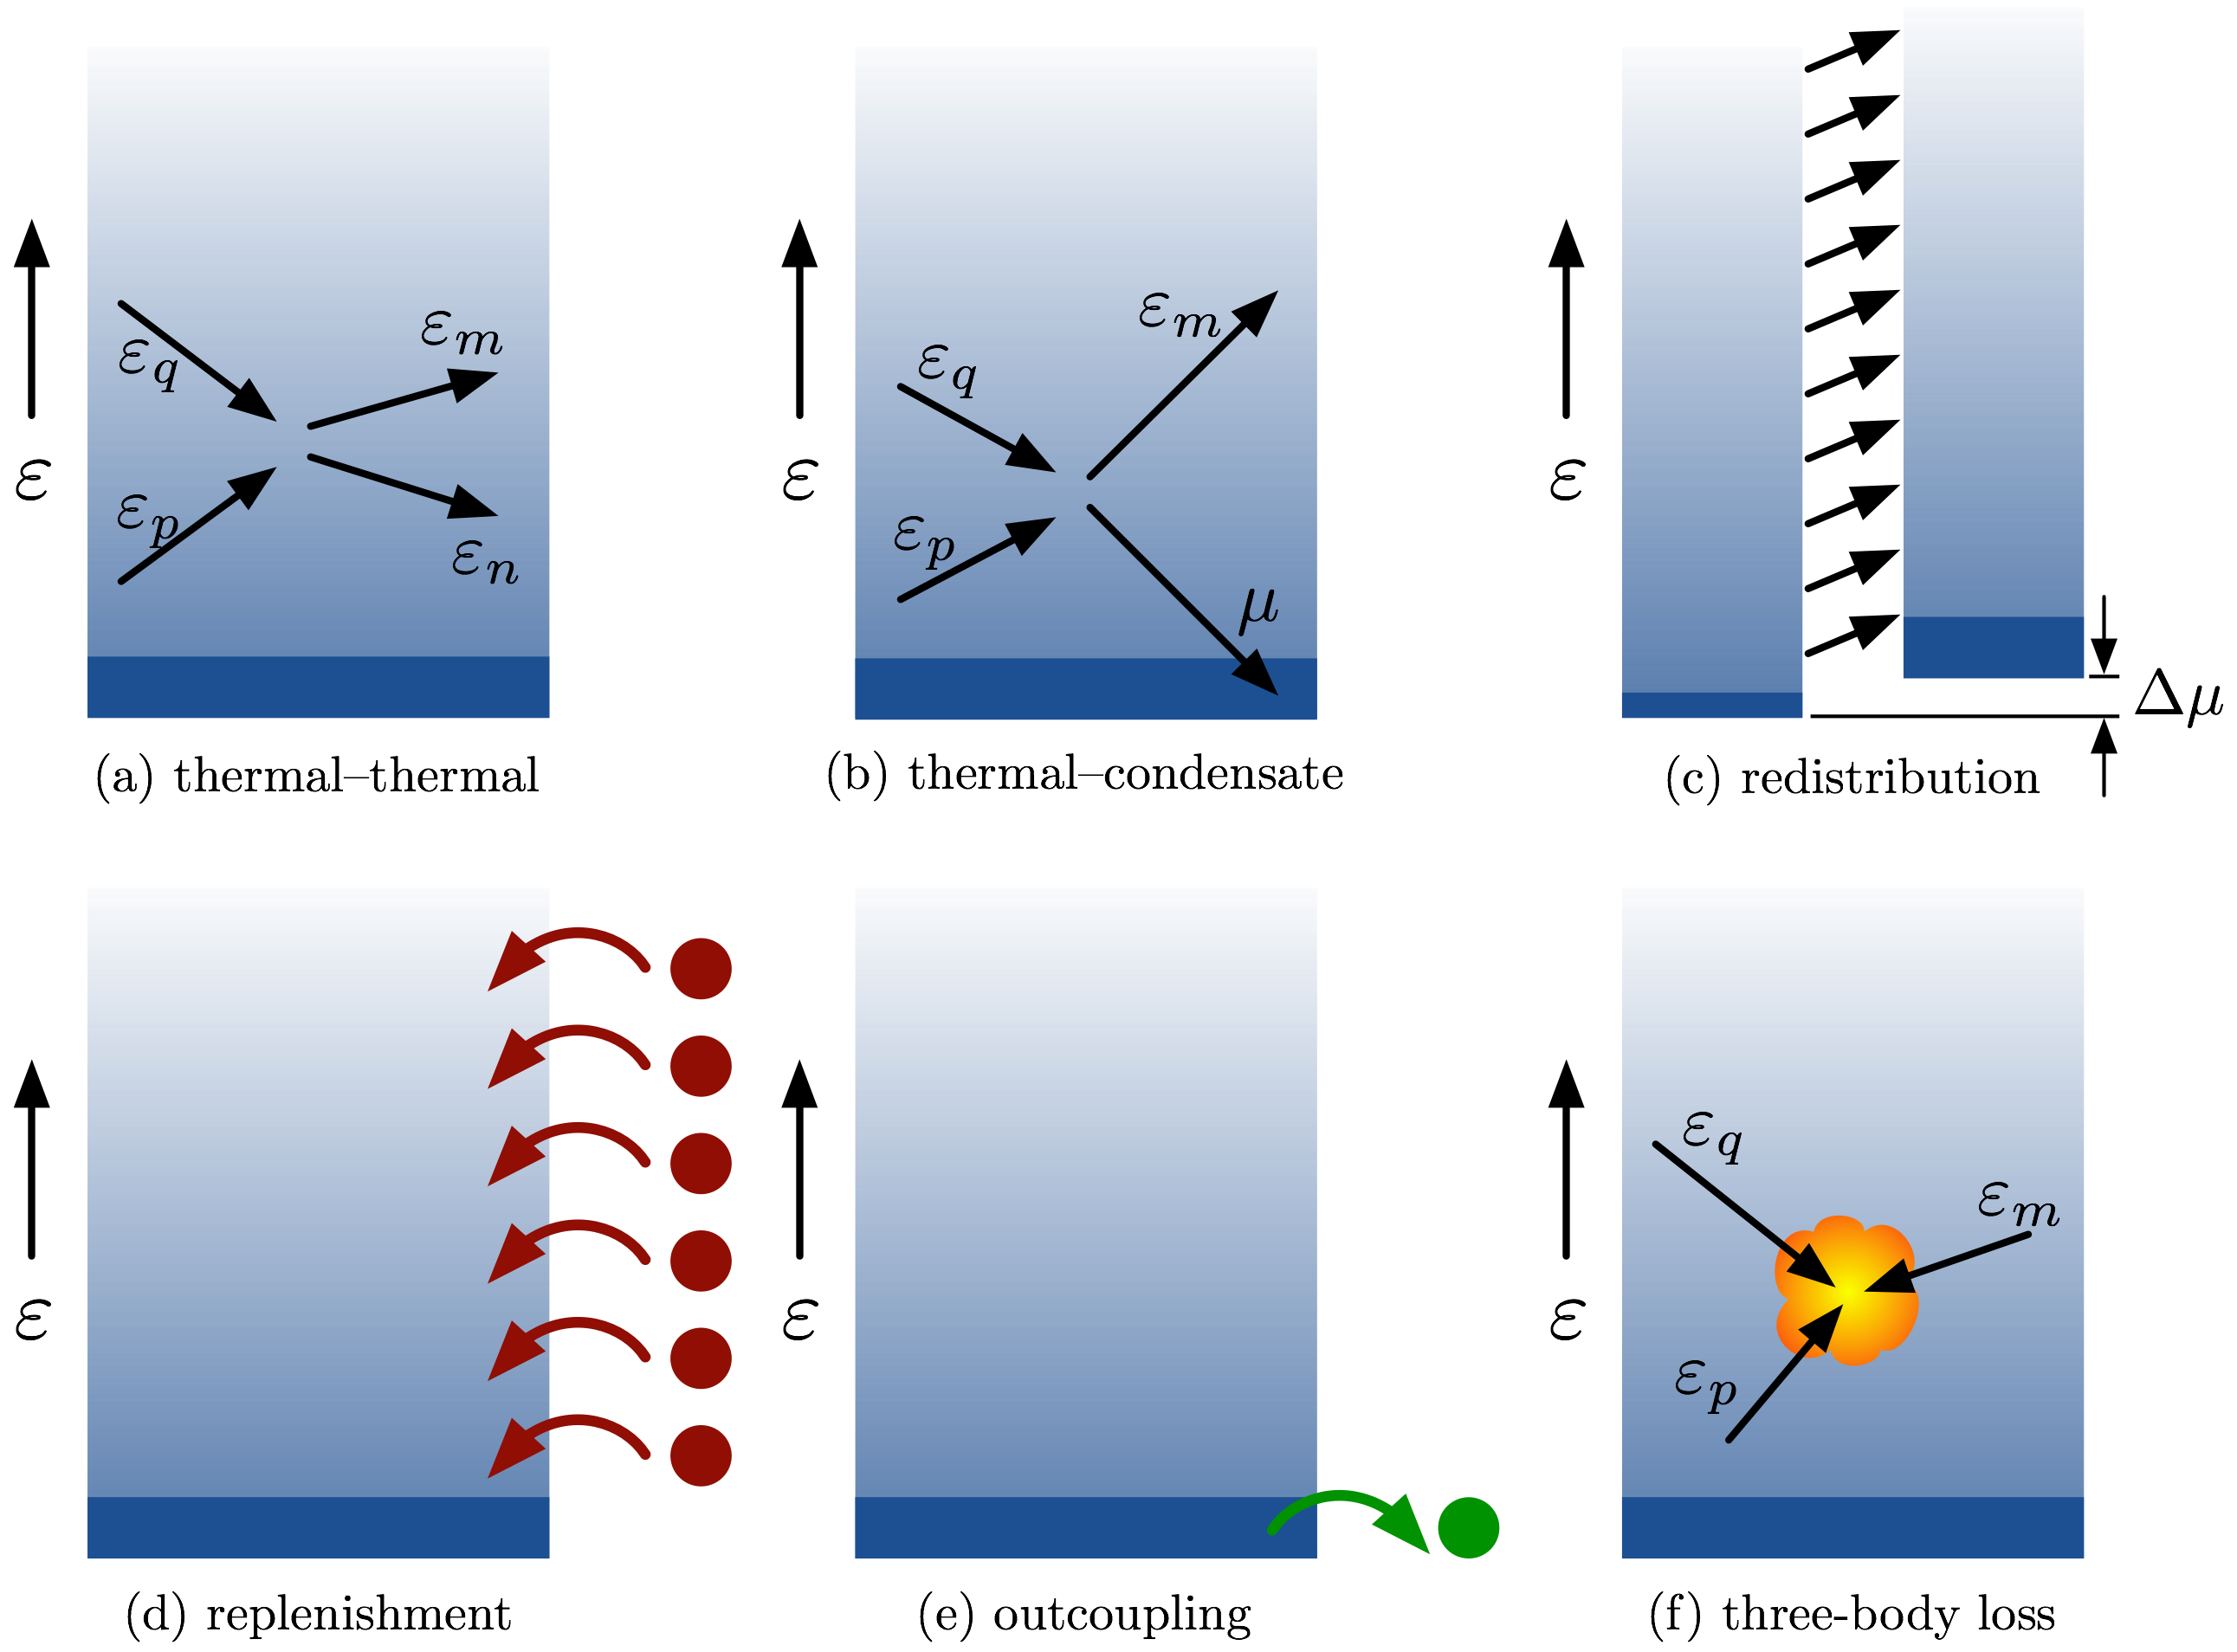
\includegraphics[width=14cm]{ProcessDiagrams}
    \caption{Schematic of processes involved in the evolution of the kinetic model described by \eqref{KineticTheory:EvolutionEquations}.  The upper shaded rectangle in each subfigure represents the energy distribution function $g(\varepsilon, t)$ of the thermal cloud, and the bottom dark blue rectangle represents the condensate with occupancy $N_0(t)$ and energy $\varepsilon = \mu(t)$. Figures (a) and (b) represent collisional processes involving two thermal atoms and one thermal and one condensate atom respectively. Figure (c) represents the change in the energy distribution function $g(\varepsilon, t)$ if the condensate occupation (and hence chemical potential) changes, changing the energies of every energy level. Figure (d) represents the replenishment of the thermal cloud from an atomic reservoir, Figure (e) represents outcoupling from the condensate mode to produce the atom laser, and Figure (f) represents the loss of atoms due to three-body recombination.}
    \label{KineticTheory:ProcessDiagrams}
\end{figure}

The forms of the `thermal--thermal', `thermal--condensate' and `redistribution' terms in \eqref{KineticTheory:EvolutionEquations} are given in \sectionref{MethodsAppendix:QKTOtherTerms} and derivations are given in~\citep{Bijlsma:2000}.

The outcoupling process from the condensate is modelled as a simple linear loss process with corresponding rate constant $\gamma$,
\begin{align}
    \left.\frac{d N_0}{d t}\right|_\text{outcoupling} &= - \gamma N_0.
    \label{KineticTheory:OutcouplingProcess}
\end{align}
In modelling the outcoupling in this way, any outcoupling from thermal modes has been neglected. As discussed in \sectionref{KineticTheory:Scheme}, this is a reasonable approximation if focused Raman lasers are used for the outcoupling which only intersect in the immediate vicinity of the condensate. 

The thermal cloud is modelled as being continuously replenished from a source that provides a constant flux $\Phi$ of atoms at a temperature $T$.  To avoid tying the model to any particular replenishment mechanism, we assume a best-case scenario in which each energy level $\varepsilon$ in the source is coupled directly to the level in the thermal cloud with the same energy above the condensate chemical potential $\mu(t)$, i.e.\ the lowest energy level of the source ($\varepsilon=0$) is coupled directly to the lowest energy level in the trap ($\varepsilon = \mu(t)$).  This simple model gives the form of the contribution due to replenishment as
\begin{align}
    \left. \frac{\partial \big(\rho(\varepsilon, t) g(\varepsilon, t)\big)}{\partial t} \right|_\text{replenishment} &= \Gamma \rho_0(\varepsilon - \mu(t)) g_T(\varepsilon - \mu(t)),
    \label{KineticTheory:ReplenishmentProcess}
\end{align}
where $\rho_0(\varepsilon)$ is the density of states in the absence of a condensate, $g_T(\varepsilon)$ is the Bose-Einstein  distribution at temperature $T$, and $\Gamma$ is a rate constant such that
\begin{align}
    \Gamma \int_0^\infty \rho_0(\varepsilon) g_T(\varepsilon)\, d\varepsilon = \Phi,
    \label{KineticTheory:GammaPhiRelation}
\end{align}
where $\Phi$ is the flux of atoms from the source \emph{before} evaporation.  The derivation of the contributions to \eqref{KineticTheory:EvolutionEquations} due to three body loss were performed by \emph{Matthew Davis}, and are given in \sectionref{MethodsAppendix:QKT3BodyLoss}.
%While this is perhaps an unreasonable assumption, it means that we can easily determine the steady state of the system.

\parasep

We summarise here the approximations made in obtaining the kinetic model \eqref{KineticTheory:EvolutionEquations}:
\begin{enumerate}[(i)]
    \item The energy scale of the thermal cloud is large enough that all excitations are particle-like and not collective excitations such as phonons. Phonon-like excitations are only important for particle energies $\varepsilon \lesssim 2\mu(t)$~\citep[\S 8.3.1]{PethickSmith}. Hence, we require that the energy scale for the thermal cloud $\varepsilon_\text{cut}$ be much larger than $\mu(t)$.
    \item The phase-space distribution of the thermal cloud is ergodic and hence is purely a function of energy. This assumption is true at equilibrium, however it needs some justification when used in non-equilibrium scenarios. In this case, asymmetric behaviour of the condensate is not expected in either position or momentum space 
    \item The condensate density is sufficiently large that it is well-described by a Thomas-Fermi profile. This approximation is justified as it is only the large-condensate limit that is of interest as a large condensate will be necessary for the production of a high-flux atom laser in this scheme. In making this approximation, the effects of both the normal and anomalous densities of the thermal cloud on the condensate have also been neglected.
    \item Evaporation occurs on a time-scale faster than collisions. This is the usual requirement during evaporation to condensation, and so should be satisfied in the proposed experiment.
\end{enumerate}

The computer code used to solve the kinetic model \eqref{KineticTheory:EvolutionEquations} was written by \emph{Matthew Davis}. The results and analysis presented in the remainder of this chapter are my own work.

\section{Simulation results}
\label{KineticTheory:Results}

For a given trap geometry, the model is fully defined by the flux of replenishment atoms $\Phi$, the temperature $T$ of those atoms, the energy of the evaporative cut $\varepsilon_\text{cut}$, and the outcoupling rate from the condensate $\gamma$. In this section the results of the kinetic model for some `typical' parameter values are presented, and the dependence of the model on each of the parameters is examined.

Our numerical simulations are based on a trap and conditions similar to that of~\citep{Kohl:2002}, who precooled a cloud of $\nucl{87}{Rb}$ atoms to an initial temperature slightly greater than the critical temperature before performing evaporative cooling to study condensate growth.  The trap in the experiment was axially-symmetric with radial and axial trapping frequencies of  $\omega_r = \unit[2 \pi \times 110]{Hz}$ and $\omega_z = \unit[2\pi \times 14]{Hz}$ respectively.

To numerically solve the kinetic model, \eqref{KineticTheory:EvolutionEquations} is discretised along the energy dimension and the resulting coupled differential equations are solved with an adaptive fourth-fifth Runge-Kutta~\citep{NumericalRecipes} method. Our results are mainly concerned with the steady-state of the kinetic model, which we define as being reached when the condensate number has changed by less than $0.1\%$ or $1$ atom in $\unit[100]{ms}$.  The initial state for the simulation is chosen to be a truncated Bose-Einstein distribution containing (before truncation) $N_\text{initial} = \unit[4.2\times 10^6]{atoms}$ at the same temperature as the replenishment reservoir.  This state is chosen as a representation of the steady-state of the system prior to evaporation.  In the trap considered, the critical temperature for $4.2\times 10^6$ atoms is $T_c = \unit[400]{nK}$.


\subsection{Typical dynamics and parameter studies}
\label{KineticTheory:ParameterStudies}

\begin{figure}
    \centering
    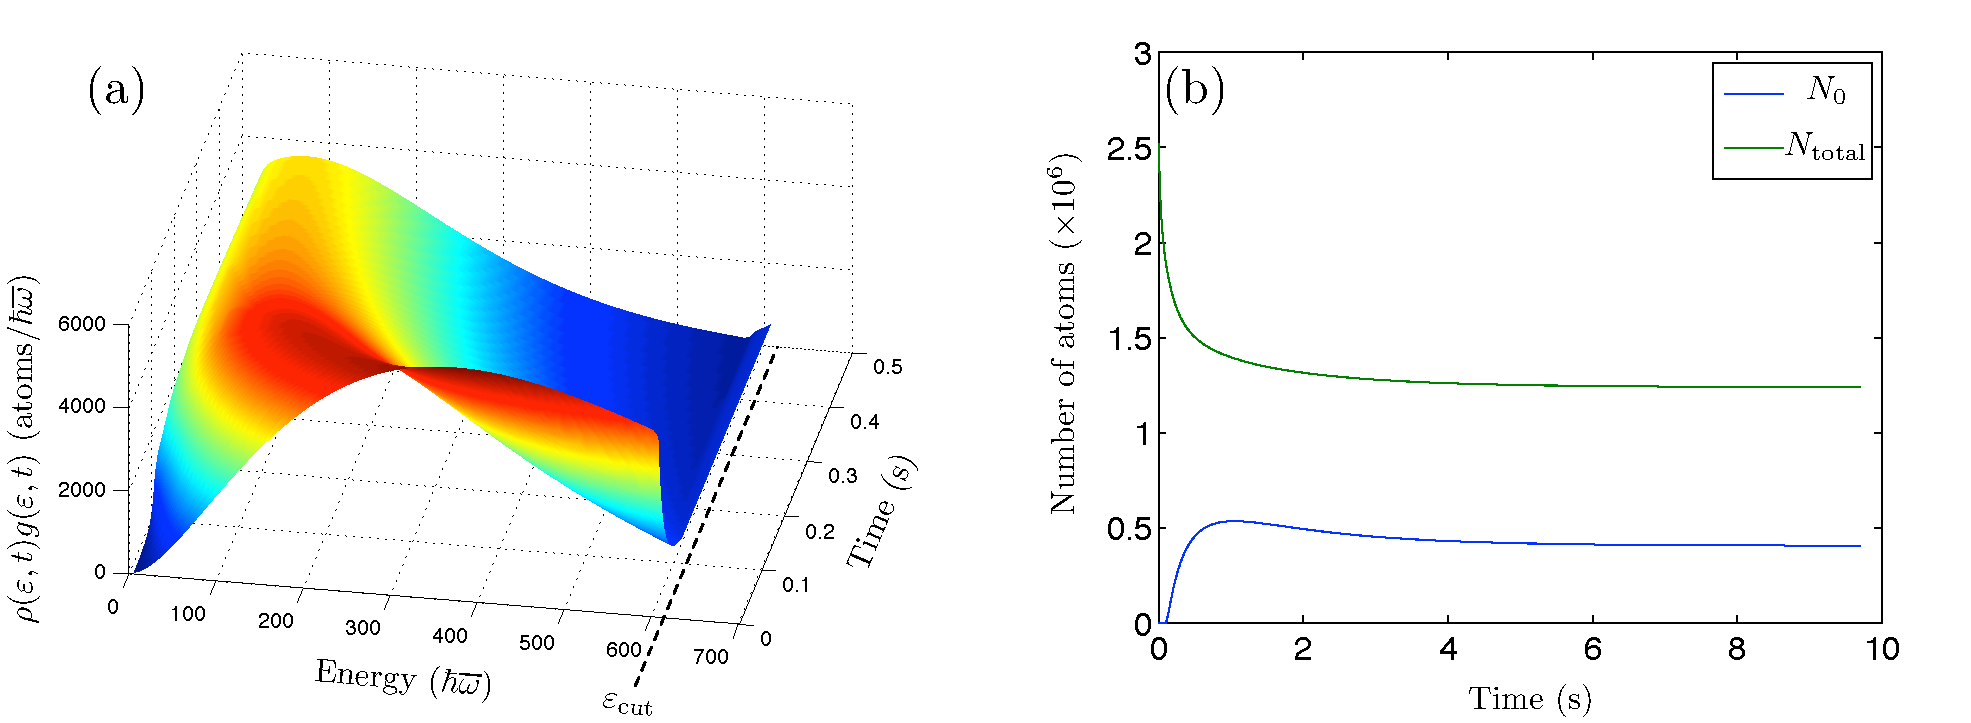
\includegraphics[width=15cm]{EnergyDistributionFunctionEvolution}
    \caption{Results of the kinetic model for $\Phi = \unit[8.4 \times 10^5]{atoms/s}$, $T=\unit[540]{nK}$, $\varepsilon_\text{cut} = 3 k_B T \approx 610 \hbar \overline{\omega}$, and $\gamma = \unit[0.3]{s\textsuperscript{-1}}$. Figure (a) highlights the dynamics of the occupation of the thermal energy levels for $t < \unit[0.5]{s}$, while (b) illustrates the equilibration of the total and condensed atom numbers over $\sim \unit[10]{s}$. The energy distribution at $t=0$ is a truncated Bose-Einstein distribution containing (before truncation) $N=4.2\times 10^6$~atoms at $T=\unit[540]{nK}$.
    }
    \label{KineticTheory:EnergyDistributionFunctionEvolution}
\end{figure}

As a depiction of the `typical' time-dependence of the results obtained from the kinetic theory model \eqref{KineticTheory:EvolutionEquations}, we consider the case of pumping the system continuously with a source such that the initial number $N = 4.2\times 10^6$ is transferred to the system once every 5 seconds giving a flux of $\Phi = \unit[8.4 \times 10^5]{atoms/s}$.  The temperature of the replenishment source is chosen to be $T=\unit[540]{nK}$, 60\% above the condensation temperature of the system before evaporation.  For the remaining model parameters, we choose the evaporative cut-off to be $\varepsilon_\text{cut} = 3 k_B T$, and the outcoupling rate from the condensate to be $\gamma = \unit[0.3]{s\textsuperscript{-1}}$.  

\figureref{KineticTheory:EnergyDistributionFunctionEvolution} illustrates the results of the simulation of this system.  \figureref{KineticTheory:EnergyDistributionFunctionEvolution}(a) shows the energy distribution of the thermal cloud cooling from the initial truncated Bose-Einstein distribution to a distribution with a lower average energy per particle.  \figureref{KineticTheory:EnergyDistributionFunctionEvolution}(b) demonstrates that despite pumping the system with an atomic reservoir above critical temperature that it is possible to reach a steady-state in which the condensate is macroscopically occupied.  In this example, the steady-state condensate fraction is 33\%.

\begin{figure}
    \centering
    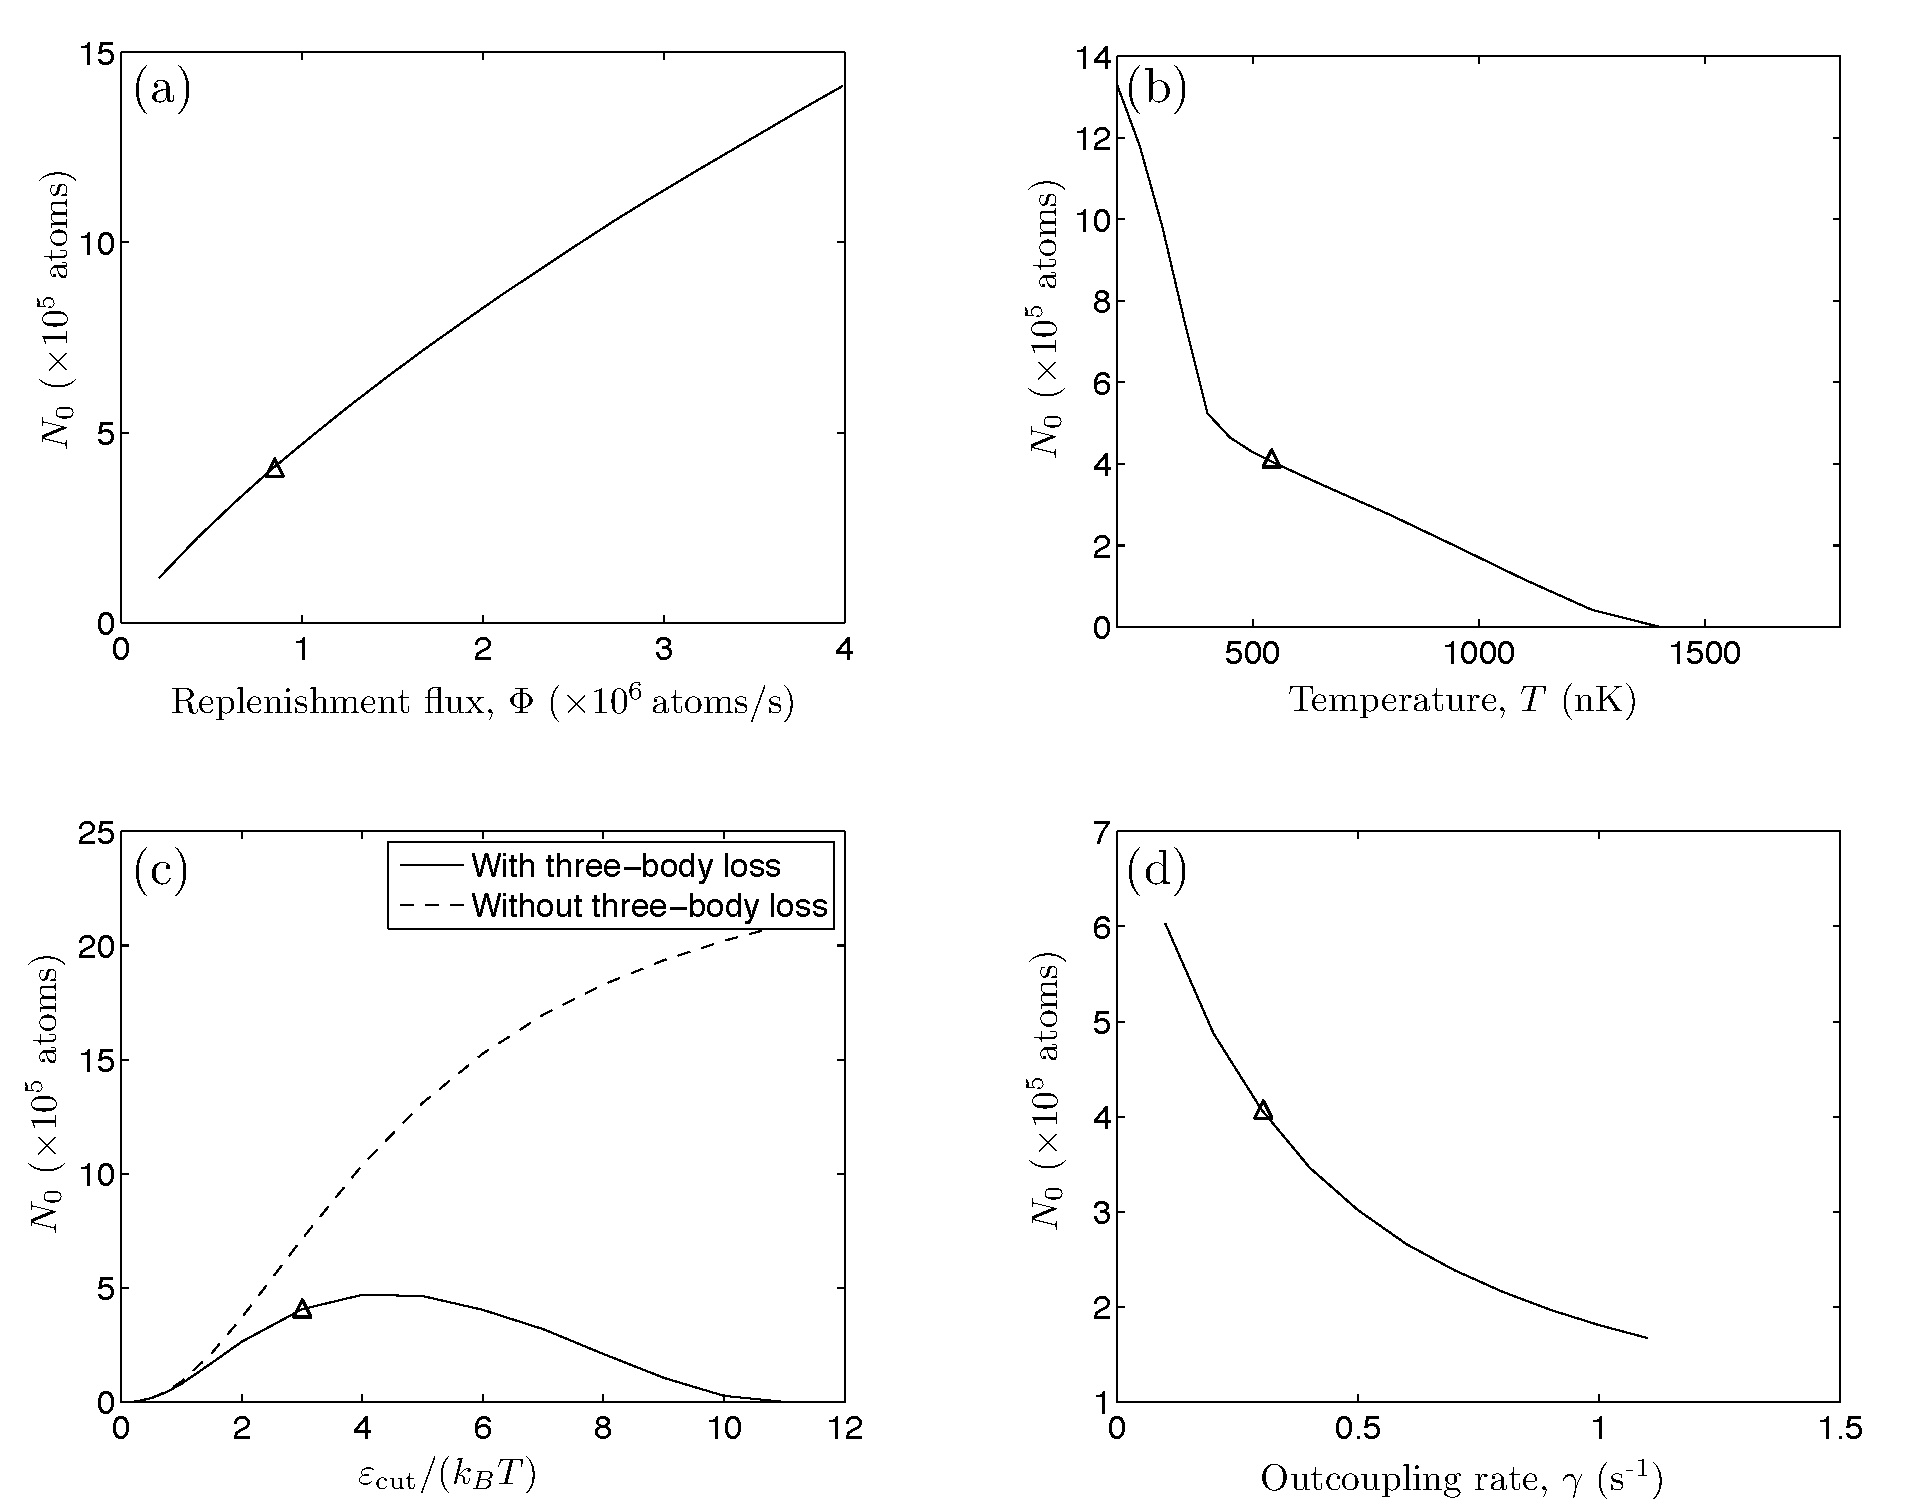
\includegraphics[width=15cm]{ParameterStudies}
    \caption{The dependence of the equilibrium condensate number $N_0$ on the parameters of the quantum kinetic model \eqref{KineticTheory:EvolutionEquations}. The equilibrium condensate number has a monotonic dependence on the replenishment flux (a), the temperature of the replenishment source (b) and the outcoupling rate (d). For a given choice of the remaining parameters of the model there is an optimum $\varepsilon_\text{cut}$ (c) for which the equilibrium condensate number is a maximum. For each parameter being varied, the remaining parameters are chosen to be the same as for the results depicted in \figureref{KineticTheory:EnergyDistributionFunctionEvolution}. The triangle in each plot marks the point that corresponds to the precise conditions of \figureref{KineticTheory:EnergyDistributionFunctionEvolution}.}
    \label{KineticTheory:ParameterStudies}
\end{figure}

The details of the equilibration of the system are not the subject of investigation here, instead our interest is in the equilibrium itself, and in determining the feasibility of creating a pumped atom laser driven by a non-condensed atomic source.  As a first step towards this investigation we consider the dependence of the equilibrium condensate number on the parameters of the system: $\Phi$, $T$, $\varepsilon_\text{cut}$, and $\gamma$.  The results of such a parameter study are presented in \figureref{KineticTheory:ParameterStudies} in which the dependence on these parameters of the steady-state of the results of \figureref{KineticTheory:EnergyDistributionFunctionEvolution} is investigated.

The majority of the parameter dependences depicted in \figureref{KineticTheory:ParameterStudies} are trivial; increasing the relevant parameter causes a monotonic change in the equilibrium condensate number.  Increasing the flux of atoms to the system increases the equilibrium condensate number [\figureref{KineticTheory:ParameterStudies}(a)], while increasing the temperature of the replenishment source or increasing the outcoupling rate reduces the equilibrium condensate number [\figureref{KineticTheory:ParameterStudies}(b) and \figureref{KineticTheory:ParameterStudies}(d) respectively].  The sharp kink in \figureref{KineticTheory:ParameterStudies}(b) occurs exactly at $T=T_c$ and is due to condensation of the source cloud.  The only non-trivial behaviour is displayed by \figureref{KineticTheory:ParameterStudies}(c) in which the dependence on the evaporative cut-off $\varepsilon_\text{cut}$ is illustrated.  For large evaporative cut-offs, few atoms will be lost due to evaporation and the system will reach equilibrium when the flux of atoms into the system is balanced by three-body losses and outcoupling from the condensate.  As $\varepsilon_\text{cut}$ is reduced, more atoms are lost due to evaporation and the mean energy per particle reduces, causing the condensate size to increase.  As $\varepsilon_\text{cut}$ continues to reduce, an increasing fraction of the replenishment atoms have an energy greater than $\varepsilon_\text{cut}$, causing a lower effective atomic flux to be delivered to the system. This reduces the potential size of any condensate formed.  These two competing effects are the origin of the existence of an optimum equilibrium condensate number as a function of $\varepsilon_\text{cut}$ in \figureref{KineticTheory:ParameterStudies}(c).

As discussed earlier, in the absence of three-body loss, the equilibrium condensate number would continue to increase as $\varepsilon_\text{cut}$ is increased, which would lead to the unphysical conclusion that evaporating \emph{reduces} the equilibrium condensate number.  This is demonstrated by the dashed line in \figureref{KineticTheory:ParameterStudies}(c) which asymptotes towards $N_0=\Phi/\gamma = \unit[2.8\times 10^6]{atoms}$ in the limit $\varepsilon_\text{cut}\rightarrow \infty$.  As observed in the remaining panels of \figureref{KineticTheory:ParameterStudies} (in which the effects of three-body loss have been included) three-body loss does not give rise to optimum values for the corresponding parameters of the model as it is only changes to $\varepsilon_\text{cut}$ that affect the evaporative and three-body losses in contrary fashions.  An increase in the replenishment flux will increase both evaporative and three-body losses.  Similarly, changes to the temperature of the replenishment source or the outcoupling rate either increase both or decrease both of the evaporative and three-body losses.

At this point the fairly obvious recommendation could be made that to have the largest equilibrium condensate number one should use a replenishment source with the highest possible flux and the lowest possible temperature.  It is an experimental reality, however, that these parameters are not orthogonal; while a $\unit[300]{K}$ oven might produce a significantly larger flux than a $\unit[50]{mK}$ 2D-MOT, it is simply not realistic to create a $\unit[50]{mK}$ atomic source with the same flux as the $\unit[300]{K}$ oven.  It is this trade-off between the temperature and flux in the context of experimentally-realisable sources that is the subject of the remainder of the chapter.

%The replenishment process could be treated in a best-case scenario in two different ways: coupling each energy levels directly that have the same energy, or coupling the nth level in one system to the nth level in the other system. The first case corresponds to rapidly combining the systems on a timescale short enough that neither system has time to react; the second case corresponds to the opposite limit in which the systems are coupled slowly enough that each energy level undergoes an adiabatic change towards the corresponding level in the other system.

% We still need more thermal sources for the high-temperature limit part of the text.


\subsection{Behaviour in the high-temperature limit}
In the previous section, the dependence of the equilibrium condensate number on the model parameters was investigated. The physical question that we desire to address with this model is what are the requirements on the replenishment source to produce a pumped atom laser?

Although it would be possible to create a pumped atom laser by combining condensates in a manner similar to the experiment by~\citet{Chikkatur:2002qa}, such an atom laser would have significantly reduced phase-stability unless the replenishment process were essentially continuous. However, to replenish a condensate by collisional interactions with a continuous source of condensed atoms, the replenishment source would itself need to have many of the desired properties of a pumped atom laser! Instead, it would be preferable to be able to use a source \emph{above} condensation temperature for replenishment.

We consider now the experimentally-relevant limit of replenishing the thermal cloud using a high-flux source of thermal atoms. For such sources two simplifications are possible. First, for temperatures greater than $T_c$ the Bose-Einstein energy distribution of the source $g_T(\varepsilon)$ is well approximated by the Boltzmann distribution $g_T(\varepsilon) \approx \zeta e^{-\beta \varepsilon}$ for some constant $\zeta$, and $\beta = \left(k_B T\right)^{-1}$. Secondly, for high temperature sources the optimum evaporation cut-off $\varepsilon_\text{cut}$ will be much smaller than the characteristic energy of the source $k_B T$, and hence $\varepsilon_\text{cut} \ll k_B T$.  From these simplifications it can be seen that the energy distribution below the evaporation cut-off is well described by the single parameter $\zeta$ as $g_T(\varepsilon \leq \varepsilon_\text{cut}) \approx \zeta$.

At this point, no overall simplification has occurred as we have simply rewritten the temperature dependence of the replenishment source in terms of the parameter $\zeta$.  However, as the energy distribution of the replenishment source only affects the kinetic model through \eqref{KineticTheory:ReplenishmentProcess}, its influence on the system dynamics is only through the combined quantity $\kappa = \Gamma \zeta$. An expression for $\kappa$ directly in terms of relevant experimental quantities can be obtained using the definition \eqref{KineticTheory:GammaPhiRelation},
\begin{align}
    \Phi &= \Gamma \int_0^\infty \rho_0(\varepsilon) g_T(\varepsilon)\, d\varepsilon \notag\\
    &= \Gamma \int_0^\infty \frac{\varepsilon^2}{2 (\hbar \overline{\omega})^3} \zeta e^{-\beta \varepsilon}\, d\varepsilon \notag\\
    &= \Gamma \zeta \frac{1}{2 (\hbar \overline{\omega})^3} \int_0^\infty \varepsilon^2 e^{-\beta \varepsilon}\, d\varepsilon \notag\\
    &= \left(\frac{k_B T}{\hbar \overline{\omega}}\right)^3 \Gamma \zeta\\
    \kappa &\equiv \Gamma \zeta = \Phi \left(\frac{\hbar \overline{\omega}}{k_B T}\right)^3 \label{KineticTheory:KappaDefinition}
\end{align}
where $\overline{\omega} = \left(\omega_x \omega_y \omega_z\right)^{\frac{1}{3}}$ is the geometric mean of the trapping frequencies, and $\displaystyle\rho_0(\varepsilon) = \frac{\varepsilon^2}{2 (\hbar \overline{\omega})^3}$ is the density of states in a harmonic trap in the absence of a condensate~\citep{PethickSmith}.

We term $\kappa$ the \emph{phase-space flux} of the source as it is directly related to the rate at which the phase-space density of the thermal source is delivered.  For a trap of $N$ thermal atoms at temperature $T$, the peak phase-space density $\varpi$ is~\citep[Chapter 2]{PethickSmith}
\begin{align}
    \varpi &= N \left(\frac{\hbar \overline{\omega}}{k_B T} \right)^3.
\end{align}
If these $N$ atoms are delivered over a time $\tau$ providing a flux $\Phi = N/\tau$ the peak phase-space flux is
\begin{align}
    \frac{\varpi}{\tau} &= \frac{N}{\tau}\left(\frac{\hbar \overline{\omega}}{k_B T}\right)^3 = \Phi \left(\frac{\hbar \overline{\omega}}{k_B T}\right)^3 \equiv \kappa.
\end{align}

The phase-space flux $\kappa$ is a figure-of-merit for the thermal source.  It quantifies the qualitative behaviour already known: for the same atomic flux $\Phi$, a source with a lower temperature will result in a larger condensate [\figureref{KineticTheory:ParameterStudies}(b)]; and for the same temperature, a source with a higher atomic flux will also result in a larger condensate [\figureref{KineticTheory:ParameterStudies}(a)].  The phase-space flux also describes exactly how a trade-off between the flux and temperature of the replenishment source will affect the equilibrium condensate number.  If two sources with different fluxes and temperatures have the same value of phase-space flux, then the equilibrium condensate number produced by the two sources will be the same (assuming the high-temperature limit applies to both sources).  Our interest is in determining what values of $\kappa$ are necessary to produce a pumped atom laser, and whether such values are achievable.

For the limit of high-temperature atomic sources, we have reduced the four variables $(\Phi, T, \varepsilon_\text{cut}, \gamma)$ required to define the model \eqref{KineticTheory:EvolutionEquations} down to three $(\kappa, \varepsilon_\text{cut}, \gamma)$. Of these three, our main interest is in the dependence of the system on the properties of the atomic source through $\kappa$. In contrast, the dependence of the equilibrium condensate number on the outcoupling rate $\gamma$ is simple [see \figureref{KineticTheory:ParameterStudies}(d)] and the results would not be expected to change qualitatively with $\gamma$. It is therefore appropriate to choose a representative value for the outcoupling rate (here $\gamma = \unit[0.3]{s\textsuperscript{-1}}$) and focus on the remaining two quantities.

As discussed in the previous section, there is an optimal choice for the evaporative cut-off $\varepsilon_\text{cut}$. Our interest here is in the best-case scenario: for a given thermal source, what is the largest condensate we can produce? To examine this question and to verify that $\kappa$ does fully describe the properties of the thermal source in the appropriate limit we have performed a parameter scan of the model \eqref{KineticTheory:EvolutionEquations} for a range of fluxes $\unit[1.3\times 10^5]{s\textsuperscript{-1}} < \Phi < \unit[5\times 10^{10}]{s\textsuperscript{-1}}$ and temperatures $2 \times\unit[10^{-7}]{K} < T < 6\times\unit[10^{-4}]{K}$ of the atomic source, for each combination determining the optimum evaporative cut $\varepsilon_\text{cut}$ to give the largest steady-state condensate number.  The results of this parameter scan are displayed in \figureref{KineticTheory:FigureOfMerit}.

\begin{figure}
    \centering
    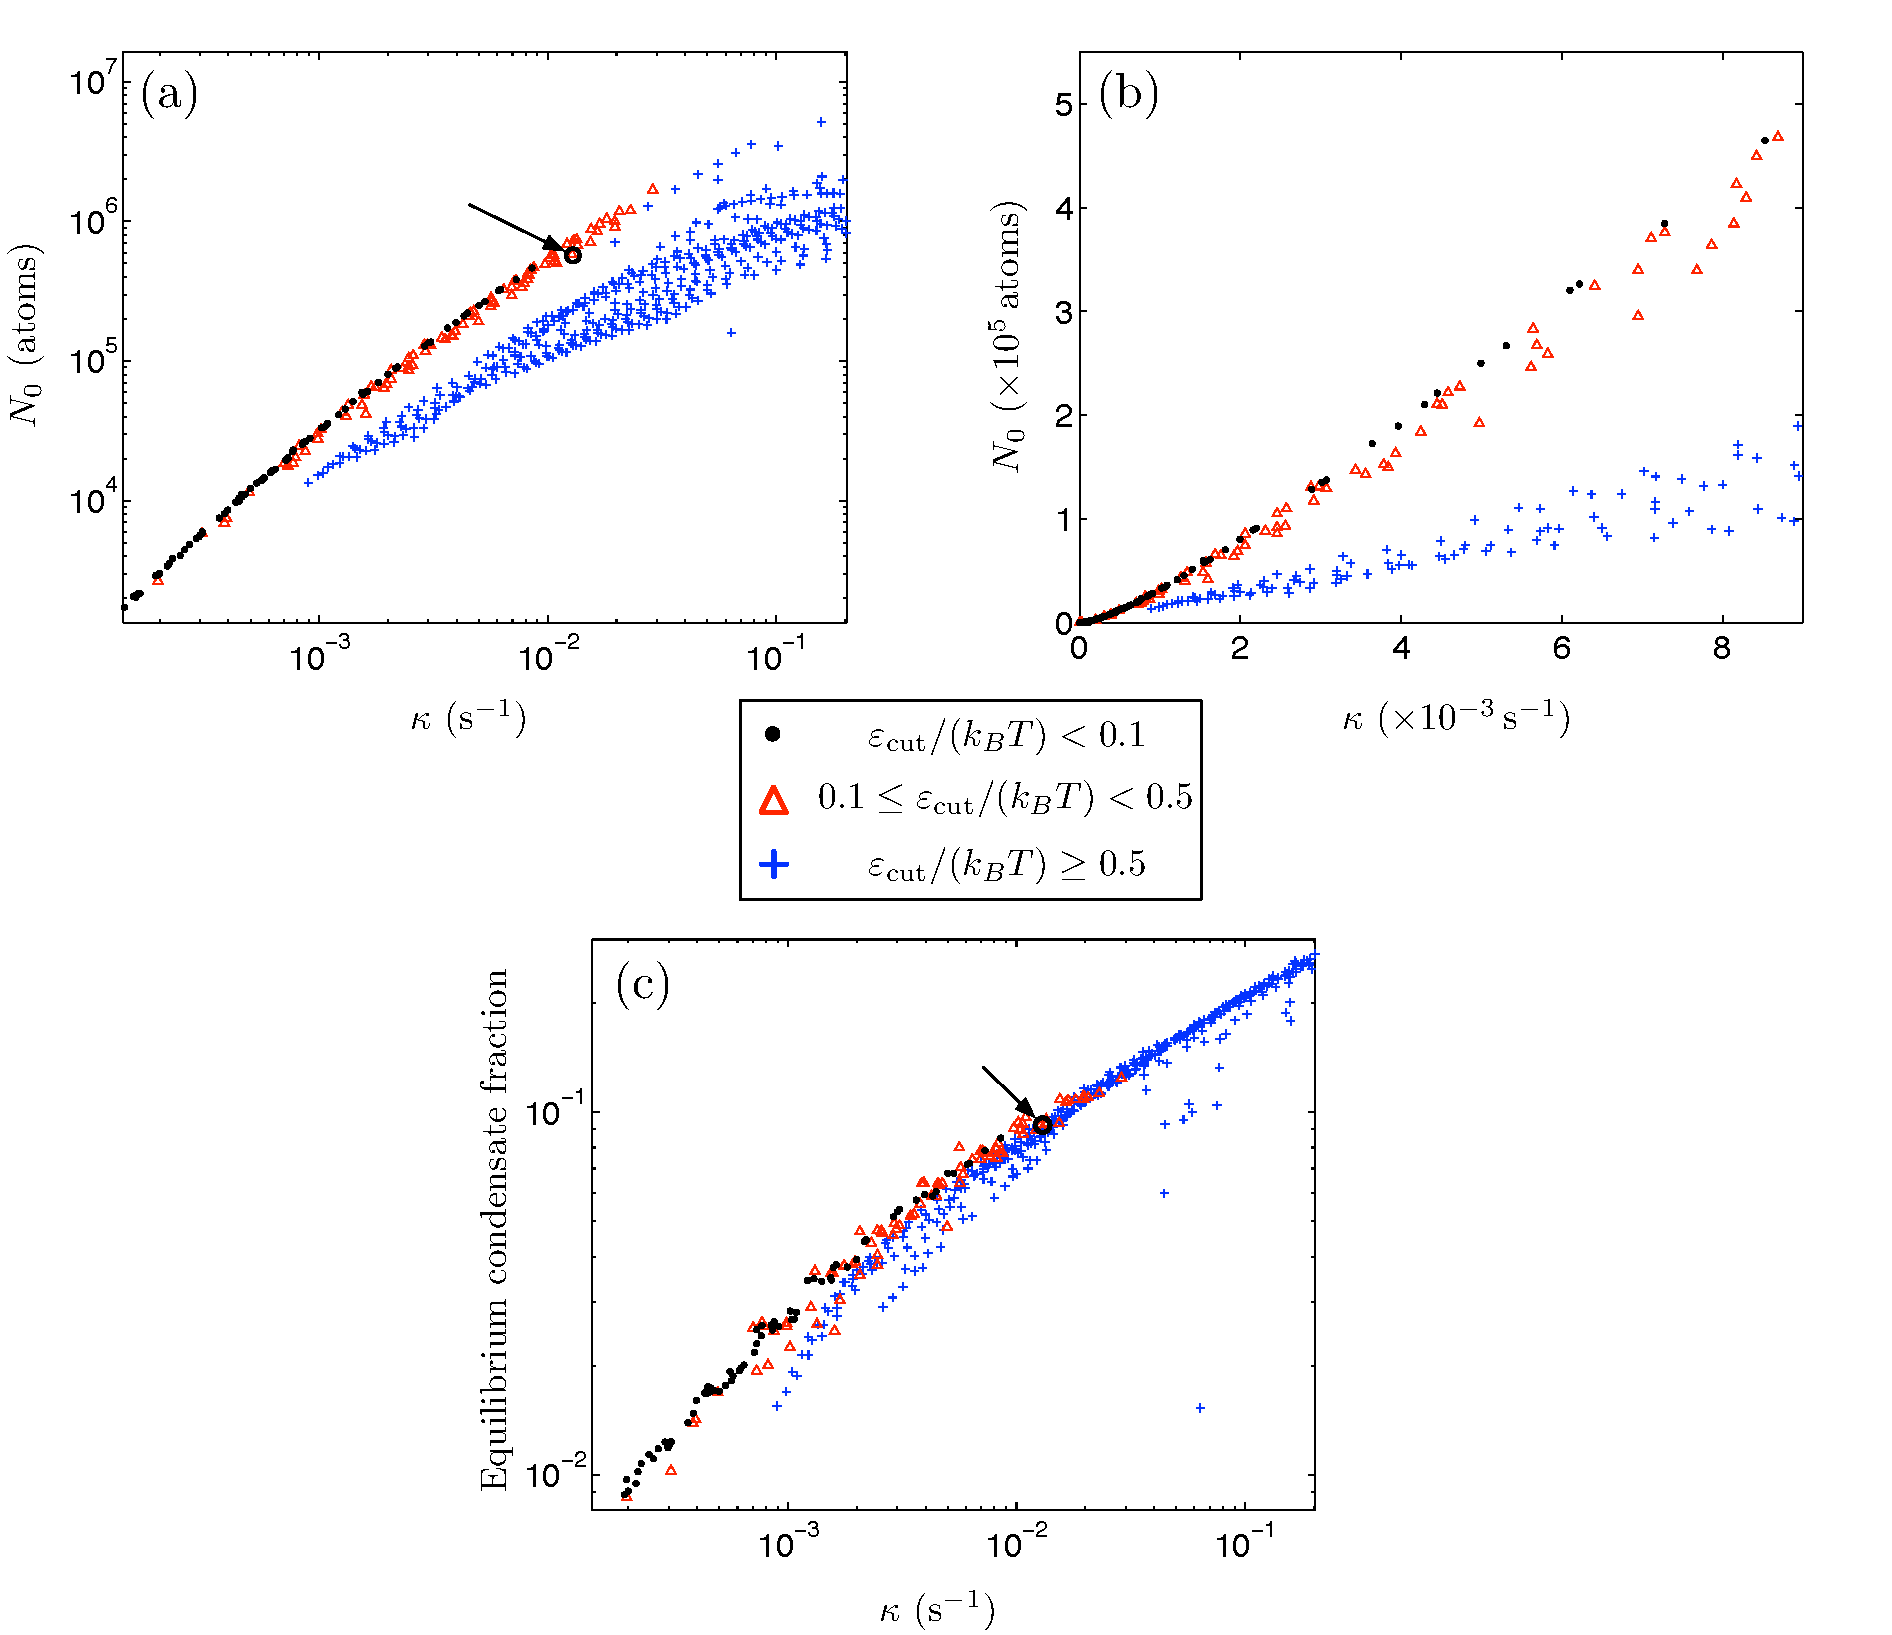
\includegraphics[width=15cm]{FigureOfMerit}
    \caption{Plot of equilibrium condensate properties as a function of the phase-space flux for the replenishment source $\kappa$. Figures (a) and (b) plot the equilibrium condensate number on different scales. Figure (c) plots the equilibrium condensate fraction $N_0/N$.  The results of the parameter scan are broken up into three groups (the black circles, red triangles and blue crosses) based on the extent to which the high-temperature limit discussed in this section applies to the results. The circled point with the arrow pointing to it corresponds to a simulation of the parameters for the last source in \tableref{KineticTheory:ExperimentalSources}, which has $\kappa= \unit[1.1\times 10^{-2}]{s\textsuperscript{-1}}$ (see main text).}
    \label{KineticTheory:FigureOfMerit}
\end{figure}

The results illustrated in \figureref{KineticTheory:FigureOfMerit} are separated into three groups based on the ratio $\varepsilon_\text{cut}/(k_B T)$.  The first group marked by black circles have $\varepsilon_\text{cut}/(k_B T) < 0.1$, and are the results for which the high-temperature limit can be considered to be a good approximation (satisfying the requirement $\varepsilon_\text{cut} \ll k_B T$) and $\kappa$ completely determines the properties of the replenishment source.  For this group of results, any equilibrium property of the system should appear to be a single (not necessarily straight) line when plotted as a function of $\kappa$.  The results in \figureref{KineticTheory:FigureOfMerit} demonstrate that these results can be viewed as a single function of $\kappa$.  The second group marked by red triangles have $0.1 \leq \varepsilon_\text{cut}/(k_B T) < 0.5$, and can be considered to be the results for which the high-temperature limit is almost a good approximation.  These results are reasonably close to the results of the first group, however there is a greater deviation for a given value of $\kappa$ indicating that the results can be almost seen as purely a function of $\kappa$. All remaining results fall into the third group for which $\varepsilon_\text{cut}/(k_B T) \geq 0.5$.  It can be seen that these points correspond to a broad range of equilibria for a given value of $\kappa$ indicating that the replenishment source cannot be described by $\kappa$ alone.
%  The origin of the distinct separation of the blue points from the red points in \figureref{KineticTheory:FigureOfMerit}(a) and \figureref{KineticTheory:FigureOfMerit}(b) is due to the use of a reduced sample of points in the three-dimensional parameter scan ($\Phi$, $T$, $\varepsilon_\text{cut}$) were used to limit the computational complexity of sampling a three-dimensional space spanning several orders of magnitude.

The first two panels of \figureref{KineticTheory:FigureOfMerit} both display the equilibrium condensate number as a function of the phase-space flux $\kappa$.  \figureref{KineticTheory:FigureOfMerit}(a) uses a log-log scale to highlight the behaviour for small and large values of $\kappa$, while \figureref{KineticTheory:FigureOfMerit}(b) uses a linear-linear scale to demonstrate that the black circles lying on a single line in (a) is not simply an artefact of plotting the results using a logarithmic scale.  Finally, \figureref{KineticTheory:FigureOfMerit}(c) displays the equilibrium condensate fraction as a function of $\kappa$.

\figureref{KineticTheory:FigureOfMerit}(a) and (b) demonstrate that it would be possible to produce atom lasers with respectable condensate numbers $N_0 \gtrsim 10^5$ (corresponding to atom laser fluxes of $\gtrsim\unit[3\times 10^4]{atoms/s}$ for the outcoupling rate $\gamma = \unit[0.3]{s\textsuperscript{-1}}$ chosen) by using replenishment sources that have a phase-space flux $\kappa \gtrsim \unit[10^{-3}]{s\textsuperscript{-1}}$.  To determine if this is experimentally feasible, the properties of a range of experimental atomic sources are detailed in \tableref{KineticTheory:ExperimentalSources} and the corresponding values of the phase-space flux $\kappa$ calculated.

\begin{table}
    \begin{minipage}{\textwidth}
        \renewcommand{\footnoterule}{}
        \centering
        \begin{tabular}{ p{3.563cm} c c c r}
        \toprule
         & Atomic flux   & Temperature  & Phase-space flux  &\\
        Atomic source &  $\Phi$  &  $T$ &  $\kappa$ &\\
        \midrule
        BECs in dipole traps & $\unit[10^5]{s\textsuperscript{-1}}$ ($\unit[55]{mHz}$)\footnote{This source is pulsed, and the flux is the mean flux over one cycle with the repetition rate listed in parentheses.}\footnote{This repetition rate it too low for this source to be useful (see main text). It is listed for purposes of comparison only.} & $<\unit[1]{\micro K}$ & $>\unit[1.9\times 10^{-3}]{s\textsuperscript{-1}}$ &~\citep{Chikkatur:2002qa} \\
        2D\textsuperscript{+}-MOT & $\unit[9\times 10^{9}]{s\textsuperscript{-1}}$ & $\unit[38]{mK}$\footnote{In keeping with the best-case scenario investigation being performed, this temperature assumes that the mean velocity of the atoms can be reduced to zero without affecting the distribution. This could be achieved, for example, by firing the source vertically below the main pumped atom laser experiment and taking the atoms from the mean turning point.}\footnote{The dominant contribution to this temperature is the spread in the longitudinal velocities of the atoms.} & $\unit[3 \times 10^{-12}]{s\textsuperscript{-1}}$ &~\citep{Dieckmann:1998} \\
        2D\textsuperscript{+}-MOT & $\unit[2\times 10^{10}]{s\textsuperscript{-1}}$ & $\unit[42]{mK}$\textsuperscript{\emph{cd}} & $\unit[5 \times 10^{-12}]{s\textsuperscript{-1}}$ &~\citep{Chaudhuri:2006} \\
        MM-MOT & $\unit[10^9]{s\textsuperscript{-1}}$ & $\unit[61]{\micro K}$\textsuperscript{\emph{c}} & $\unit[8 \times 10^{-5}]{s\textsuperscript{-1}}$ &~\citep{Cren:2002rt}\\
        LVIS & $\unit[5\times 10^{9}]{s\textsuperscript{-1}}$ & $\unit[25]{mK}$\textsuperscript{\emph{cd}} & $\unit[6 \times 10^{-12}]{s\textsuperscript{-1}}$ &~\citep{Lu:1996} \\
        Zeeman slower & $\unit[3.2\times 10^{12}]{s\textsuperscript{-1}}$ & $\unit[32]{mK}$\textsuperscript{\emph{cd}} & $\unit[2\times10^{-9}]{s\textsuperscript{-1}}$ &~\citep{Slowe:2005} \\
        Magnetic guide loaded from 3D-MOT & $\unit[7\times 10^{9}]{s\textsuperscript{-1}}$ & $\unit[400]{\micro K}$\textsuperscript{\emph{c}} & $\unit[2\times 10^{-6}]{s\textsuperscript{-1}}$ &~\citep{Lahaye:2004}\\
        3D-MOT loaded from Zeeman slower & $\unit[2\times 10^{10}]{s\textsuperscript{-1}}$ ($\unit[0.5]{Hz}$)\textsuperscript{\emph{a}} & $\unit[500]{\micro K}$ & $\unit[3\times 10^{-6}]{s\textsuperscript{-1}}$ &~\citep{Streed:2006}\\
        3D-MOT loaded from 2D\textsuperscript{+}-MOT & $\unit[3\times 10^8]{s\textsuperscript{-1}}$ ($\unit[3]{Hz}$)\textsuperscript{\emph{a}} & $\unit[8]{\micro K}$ & $\unit[1.1\times 10^{-2}]{s\textsuperscript{-1}}$ &~\citep{Muller:2007}\\
        \bottomrule
        \end{tabular}
    \end{minipage}
    \caption{Relevant properties of selected experimental cold atomic sources. The phase-space flux $\kappa$ is evaluated from the atomic flux and temperature values listed using \eqref{KineticTheory:KappaDefinition}.}
    \label{KineticTheory:ExperimentalSources}
\end{table}

The first source listed in \tableref{KineticTheory:ExperimentalSources} is the experiment by~\citet{Chikkatur:2002qa} that merged independently produced BECs in optical dipole traps that was discussed earlier.  This experiment is certainly not in the high-temperature limit, but it has been included for comparison purposes.  Of the remaining sources listed in \tableref{KineticTheory:ExperimentalSources}, most are many orders of magnitude away from being useful potential sources for a pumped atom laser (cf. \figureref{KineticTheory:FigureOfMerit}).  The fluxes obtainable from these sources are insufficient to compensate for their higher temperatures. An increase of three-orders of magnitude in flux is necessary to compensate for an increase of a single order of magnitude in temperature [see \eqref{KineticTheory:KappaDefinition}].  Only the last atomic source satisfies the requirement $\kappa \gtrsim \unit[10^{-3}]{s\textsuperscript{-3}}$.  This experiment by~\citet{Muller:2007} is one of the sources in a dual atom interferometer designed for the precision measurement of accelerations and rotations~\citep{Muller:2009}.  A direct simulation has been performed for the parameters of this source, and the results are marked by a circle with an arrow pointing to it in \figureref{KineticTheory:FigureOfMerit}.  

The equilibrium condensate number for the source of~\citet{Muller:2007} is $N_0 = \unit[5 \times 10^5]{atoms}$, which would be a sufficiently large condensate to serve as a stable phase-reference for a produced atom laser were it a pure BEC.  However the equilibrium condensate fraction for this source is only 10\% [see \figureref{KineticTheory:FigureOfMerit}(c)].  With 90\% of the atoms in the thermal cloud, one cannot help but suspect that the significant thermal fluctuations would rule out the use of any atom laser produced by this source for interferometric use, which was our original motivation.  However, previous theoretical work investigating the transfer of statistics from a trapped (quasi-)condensate to an atom laser found that using high-momentum kick Raman outcoupling such as that proposed in the scheme presented here can filter some of these fluctuations causing the atom laser to have a larger coherence length than the condensate from which it was produced~\citep{Proukakis:2003}.  

It is not possible to investigate the transfer of statistics from the trapped component to the atom laser within the present model due to the simplifying assumption that it is only the condensate mode that is outcoupled to form the atom laser.  A more detailed three-dimensional model taking into account the full spatial dependence of the Raman outcoupling process would be necessary to fully determine the feasibility of using an atomic source such as that described by~\citet{Muller:2007} in the production of a truly continuous pumped atom laser.

%The equilibrium condensate number for the source of~\citet{Muller:2007} is $N_0 = \unit[5 \times 10^5]{atoms}$, which is a sufficiently large condensate to serve as a stable phase-reference for the produced atom laser.  However, the equilibrium condensate fraction is a mere 10\%.  This number is concerning as with 90\% of the atoms in the thermal cloud, it would be expected that there would be significant thermal fluctuations on any atom laser extracted.  Although the transfer of thermal fluctuations cannot be investigated in the kinetic model presented here, it seems reasonable to believe that thermal fluctuations would dominate the linewidth of the atom laser produced.  \figureref{KineticTheory:FigureOfMerit}(c) suggests that the situation won't be significantly improved if the atomic flux were increased by an order of magnitude. In this case with $\kappa \sim 10^{-1}$, the condensate fraction would have only increased to 20\%.  The temperature of the source cannot be reduced greatly either as at $T=\unit[8]{\micro K}$, it is not very far above the condensation temperature of the system of $T_c=\unit[1.2]{\micro K}$ for each $N=10^8$ atom pulse.



%Although this source is not quite in the high-temperature limit (the optimum evaporation cut-off is $\varepsilon_\text{cut} = 0.42 k_B T$)


\section{Conclusion}

The purpose of this chapter has been to investigate the feasibility of producing a continuously pumped atom laser driven by  collisions with a cloud of thermal atoms.  The method has been to investigate the best-case scenario in which the replenishment process introduces no heating to the trapped thermal component beyond that due to bringing the replenishing atoms into contact with the thermal cloud.  With these caveats in mind, the results are promising: using an existing experimental source~\citep{Muller:2007} it appears possible to produce steady-state condensates with large atom number ($\sim 5\times 10^5$ atoms) using the scheme presented in \sectionref{KineticTheory:Scheme}.  Should the atomic flux of this source be increased by an order of magnitude, the condensate number produced by this scheme could be pushed to $5\times 10^6$ atoms.  

Ultimately it is not the size of the condensate that we are interested in, but the flux of the atom laser produced and its coherence length.  The former goal will certainly be improved by larger equilibrium condensate sizes, however the atom laser itself will be useless unless its coherence length is sufficiently larger than that of cold thermal sources to offset its necessarily lower atom flux.  The model used in this chapter cannot answer the latter question.  To investigate this further it will be necessary to include the full multimode behaviour of the Raman outcoupler and the fluctuations of the thermal cloud.  This can be achieved through using a more general kinetic theory such as the `ZNG theory'~\citep{Zaremba:1999,Proukakis:2008} or the Stochastic Projected Gross-Pitaevskii equation (SPGPE)~\citep{Blakie:2008a}.

% One thing is certainly clear from the results presented here: the replenishment source for a collisionally-pumped atom laser must be close to degeneracy. It is simply not realistic to compensate for higher temperatures with a sufficiently increased flux.

% The author is cautiously optimistic about the promise of atom lasers replenished directly from thermal sources. Though this is not the only option for the production of a continuous atom laser.  Optical pumping, discussed in \chapterref{OpticalPumping} is another option, as is evaporation of an atomic beam in a magnetic guide~\citep{Mandonnet:2000lr,Lahaye:2004,Lahaye:2005uq}.




\chapter{Conclusion}
\label{Conclusion}
\graphicspath{{Figures/Conclusion/}{Figures/Common/}}

Is it possible to produce a continuous coherent atomic source with sufficient flux to be viable for use in atomic interferometry?  That is the question that this thesis has sought to contribute to.  For the specific realisations of the pumping mechanisms considered in this thesis, the answer is no; the answer to the question more generally is less clear.  

For the optical pumping mechanism considered in \chapterref{OpticalPumping}, the achievable flux of the atom laser is limited by the rate at which condensates can be produced to replace the source condensate as it is depleted.  Even if all of the atoms were transferred to the lasing condensate with perfect efficiency, the continuous atom laser produced could never exceed the average flux with which the source condensates can be produced.  The optical pumping experiment described in that chapter is therefore not a useful source for atom interferometry in its present form.  However, there is some evidence that the harmful reabsorption processes in that experiment may be suppressed.  A better theoretical understanding of this process would determine whether or not the source condensate could be replaced with a thermal source instead.  If possible, this would greatly increase the potential flux of the produced atom laser.

The evaporatively-driven pumping mechanism considered in \chapterref{KineticTheory}, is supplied by a thermal source and could therefore provide a condensed source of atoms at a similar flux to the thermal source.  However, the actual flux is necessarily lower as atoms are removed from the system in the pumping mechanism due to the evaporation process.  The maximum theoretically achievable flux for an atom laser based on this pumping mechanism using an available thermal atomic source was $\sim\unit[10^5]{s\textsuperscript{-1}}$, an average flux which is also achievable by producing independent condensates.

While neither of the proposed pumped atom lasers are competitive with thermal sources for atom interferometry, pumping could improve other atom laser experiments.  In particular, experiments in which squeezing or entanglement of atomic beams is being produced and measured.  In these situations, a thermal source is inadequate, and a condensed source is necessary.  For these experiments, a pumped atom laser could potentially offer the narrow linewidth and continuous operation necessary to increase the sensitivity of measurements of squeezing and entanglement.  Now we move on to a discussion of Peaks.

Despite this bleak outlook, this thesis has some more positive conclusions.  

Peaks:

In this chapter, an unusual process in an atom laser was investigated.  The process involved the direct conversion of mean-field energy to the kinetic energy of unstable modes in the condensate.  This process was shown to generate entanglement in certain regimes, although in the experiment discussed it is unlikely that this entanglement remains in the outcoupled atom laser, and certainly not in any useful form.  These problems are however not fundamental.  A differently-designed experiment could overcome some of these problems to potentially produce entangled atom lasers.

The below is a positive conclusion:

One possibility worthwhile investigating would be to use a highly elongated two-state condensate in which both states experience the same trapping potential.  This could be achieved for example through the use of an optical dipole trap.  As the two states of the condensate would experience the same trapping potential, the two components of the dynamical instabilities would propagate together, avoiding the problem of one of the components of the entangled modes leaving the condensate without the other.  Further, due to the high aspect ratio, the instabilities would propagate solely along the axial dimension.  To extract the entangled beams, one would need to turn off the optical dipole trap after a given interaction time.  The atoms would then expand ballistically, with the entangled beams spatially separating from the main condensate due to their large momentum in the axial direction.  This experiment may then enable the production of highly-directional entangled atom lasers.  Further theoretical investigation would be necessary to determine if such an experiment were feasible.


Optical pumping:

There are three parts to the optical pumping process underlying the pumping experiments discussed in this chapter:
\begin{enumerate}[(i)]
    \item the delivery of atoms in an appropriate mode to the lasing condensate;
    \item the transfer of those atoms into the lasing condensate; and
    \item the propagation of the emitted photons within the lasing condensate.
\end{enumerate}
This chapter has aimed to understand part (ii) of this process.  Ideally we would also like to understand (iii) as it appears that there is some very interesting physics occurring there (at least for the $2 \hbar k$ momentum-transfer process), however there is strong experimental evidence that physics beyond the mean-field are significant in this part of the process and more detailed theoretical modelling will be necessary to accurately describe this part of the process.  By contrast process (i) is a detail determined by how one chooses to get the atoms to the lasing condensate with an appropriate mode.  While it can be argued that this process is well understood in the context of the pulsed pumping experiment, significant approximations were used for the case of the continuous pumping experiment.  While the details of the transfer of atoms into an appropriate source mode for the pumping mechanism are of course important, they are not of fundamental importance to the pumping mechanism.

One of the questions relevant to the continuous pumping experiment that we investigated theoretically was whether it was the $0 \hbar k$ or $2 \hbar k$ momentum-transfer process operating in the experiment.  While theoretically we were unable to find a regime in which the $2 \hbar k$ momentum-transfer process delivered efficient pumping, there is experimental evidence (see \citep{Doring:2009} for details) that the outcoupling position in the continuous pumping experiment was closer to the centre of the source condensate, not near the edge of the condensate as necessary for the operation of the $0 \hbar k$ momentum-transfer process.  As discussed in the previous section, it may be due to the neglect of the reabsorption process that the $2 \hbar k$ momentum-transfer process was not found to operate efficiently.  This does not discount the result that the $0 \hbar k$ momentum-transfer process \emph{can} operate.  As the photons are emitted at the edge of the condensate and propagate away reabsorption does not significantly affect this process.  It is somewhat surprising that there is a regime in which a resonant optical pumping process can be operated in which the resonant photons do not get the chance to interact significantly with the lasing condensate.

The comparison of theoretical and experimental results suggests that physics beyond the mean field are significant in the $2 \hbar k$ momentum-transfer process, which is certainly operating at least in the pulsed pumping experiment.  Further investigation of the counter-intuitive possibility that reabsorption may decrease heating resulting from spontaneous emission is certainly warranted.  The next step in this process would be to theoretically model and solve the full 3D atom--light system treating spontaneous emission and reabsorption fully.  This will be a computationally intensive process and too prohibitive to apply to the continuous pumping experiment.  However it could reasonably be applied to the pulsed pumping experiment where the optical degrees of freedom only need to be included during the short time for which the pumping light is applied.  The fall of the atomic pulses under gravity may be treated separately using standard techniques.

The complication resulting from the reabsorption of resonant photons does not arise when the applied optical pumping light is significantly detuned.  In this limit it has been shown that in a simple atom laser model pumping efficiencies of about 50\% are achievable.  It is interesting to note that the relative propagation direction of the emitted light and atom laser can have a significant effect on the efficiency of the pumping process in the detuned limit.  Although practical operation in this model was limited to the $0 \hbar k$ momentum-transfer process, both processes may be feasible in a model closer to the continuous pumping experiment in which the effects of gravity are included.  In such a model the atom laser will only be momentum-resonant with the lasing condensate for a short amount of time, reducing the possibility that multiple Rabi oscillations will limit the efficiency (refer to \figureref{OpticalPumping:TravellingBeamFarDetunedResults}).  This would be a straightforward extension of the present work.


The below is a positive conclusion:

Contrary to what has been expected previously, this chapter has demonstrated that optical pumping of an atom laser is feasible without making the condensate so narrow as to make it essentially transparent in at least one dimension.  The next step in the investigation of this pumping process must be the theoretical consideration of the potential positive contribution of reabsorption.  When this is better understood, consideration can then be given to the integration of the pumping mechanism with a method for replacing the source condensates to produce a continuously pumped atom laser.


Kinetic Theory:

The purpose of this chapter has been to investigate the feasibility of producing a continuously pumped atom laser driven by  collisions with a cloud of thermal atoms.  The method has been to investigate the best-case scenario in which the replenishment process introduces no heating to the trapped thermal component beyond that due to bringing the replenishing atoms into contact with the thermal cloud.  With these caveats in mind, the results are promising: using an existing experimental source~\citep{Muller:2007} it appears possible to produce steady-state condensates with large atom number ($\sim 5\times 10^5$ atoms) using the scheme presented in \sectionref{KineticTheory:Scheme}.  Should the atomic flux of this source be increased by an order of magnitude, the condensate number produced by this scheme could be pushed to $5\times 10^6$ atoms.  

Ultimately it is not the size of the condensate that we are interested in, but the flux of the atom laser produced and its coherence length.  The former goal will certainly be improved by larger equilibrium condensate sizes, however the atom laser itself will be useless unless its coherence length is sufficiently larger than that of cold thermal sources to offset its necessarily lower atom flux.  The model used in this chapter cannot answer the latter question.  To investigate this further it will be necessary to include the full multimode behaviour of the Raman outcoupler and the fluctuations of the thermal cloud.  This can be achieved through using a more general kinetic theory such as the `ZNG theory'~\citep{Zaremba:1999,Proukakis:2008} or the Stochastic Projected Gross-Pitaevskii equation (SPGPE)~\citep{Blakie:2008a}.


I need specific conclusions that can be drawn from the thesis, and a brief discussion of future work.  I should make some positive noises about thermal pumping.  I should make some noises about just how many orders of magnitude in flux need to be gained to reach the same level as the cold atomic sources currently used in atom interferometers.  After all, atom interferometry was the stated motivation at the start of this thesis.

On optical pumping: the result is far less clear.  Optical pumping is certainly hard, due to the dispersion relation problems discussed in the Introduction, but there are some interesting behaviours occurring in the pumping systems that warrant further investigation.  While perhaps less satisfying, the results are intriguing.

On entangled beams: the system is not sufficiently clean to be used as a source of entangled atomic beams.  Other problems discussed with Rob would seem to prevent the system being used for quasi-continuous sources either.  Pulsed mode appears to be the best we can do.  We have, however, demonstrated good agreement between theory and experiment, and that must count for something.

Transverse profile:  Large interaction strengths are likely to be a problem.  Interactions are, however, necessary in the evaporation to BEC.  This can be controlled through the use of a Feschbach resonance.  Other work has demonstrated that the atom laser can be guided to a high degree.


\appendix
\chapter{Elementary excitations of temporally periodic Hamiltonians}
\label{FloquetAppendix}
\graphicspath{{Figures/FloquetAppendix/}{Figures/Common/}}

\section{Evolution of the excitations}
\label{FloquetAppendix:Evolution}
The theory of elementary excitations in unstable Bose-Einstein Condensates has been considered before~\citep{Leonhardt:2003}.  In this section, restrictions on the Floquet exponents for the system under consideration in \sectionref{Peaks:PerturbativeApproach} are obtained, from which the equations of motion for the instabilities may be solved.  This is achieved by applying the methods discussed in \citep{Leonhardt:2003} and consideration of the symmetries of the system Hamiltonian.  This Hamiltonian can be obtained by making a perturbative expansion of the Hamiltonian \eqref{Peaks:InitialHamiltonian} about the time-dependent (but periodic) mean-field.

Consider a general quadratic, spatially-homogeneous Hamiltonian $\hat{H}(t)$ of period $T$ in terms of the operators $\hat{\phi}_i(\vect{x}, t)$ which obey the usual equal-time bosonic commutation relations. As the Hamiltonian $\hat{H}(t)$ is homogenous by assumption, the operator equations of motion will take their simplest form in a Fourier basis. In this basis the equations of motion for the operators $\hat{\phi}_i(\vect{k}, t)$ can be written in matrix form\footnote{Due to conservation of momentum, the Hamiltonian $\hat{H}(t)$ can only contain terms of the form $\hat{\phi}_i^\dagger(\vect{k}, t) \hat{\phi}_j^{\phantom{\dagger}}(\vect{k}, t)$, $\hat{\phi}_i^\dagger(\vect{k}, t) \hat{\phi}_j^{\dagger}(-\vect{k}, t)$ and $\hat{\phi}_i^{\phantom{\dagger}}(\vect{k}, t) \hat{\phi}_j^{\phantom{\dagger}}(-\vect{k}, t)$. Consequently the terms $\hat{\phi}_j(-\vect{k}, t)$ and $\hat{\phi}_j^\dagger(\vect{k}, t)$ cannot occur on the RHS of \eqref{FloquetAppendix:UpsilonEquationOfMotion}.},
\begin{subequations}
    \label{FloquetAppendix:MatrixOperatorEvolution}
    \begin{align}
        i \hbar \frac{\partial }{\partial t}\hat{\vect{\Upsilon}}(\vect{k}, t) &= \mathcal{H}(\vect{k}, t) \hat{\vect{\Upsilon}}(\vect{k}, t), \label{FloquetAppendix:UpsilonEquationOfMotion}\\
        \hat{\vect{\Upsilon}}(\vect{k}, t) &= 
        \begin{pmatrix}
            \hat{\phi}_1^{\phantom{\dagger}}(\vect{k}, t) &
            \hat{\phi}_1^\dagger(-\vect{k}, t) &
            \hat{\phi}_2^{\phantom{\dagger}}(\vect{k}, t) &
            \hat{\phi}_2^\dagger(-\vect{k}, t) &
            \dots
        \end{pmatrix}^\text{T},
    \end{align}
\end{subequations}
where the matrix $\mathcal{H}(\vect{k}, t)$ obeys
\begin{align}
        \mathcal{H}(\vect{k}, t+T) &= \mathcal{H}(\vect{k}, t),\\
        \mathcal{H}(\vect{k}, t) &= \mathcal{H}(-\vect{k}, t), \label{FloquetAppendix:HReflectionSymmetry}
\end{align}
where the last equality holds because $\hat{H}(t)$ is isotropic.

If the Hamiltonian $\hat{H}(t)$ were not time-dependent, $\mathcal{H}(\vect{k}, t)$ could be diagonalised to find the (potentially complex) eigenvalues $\Omega_j(\vect{k})$ and corresponding operators $\hat{Q}_j(\vect{k}, t)$ which would evolve as
\begin{align}
    \label{FloquetAppendix:ContinouousTimeEigenoperators}
    i \hbar \frac{\partial }{\partial t}\hat{Q}_j(\vect{k}, t) &= \hbar \Omega_j(\vect{k}) \hat{Q}_j(\vect{k}, t),
\end{align}
where the $\hat{Q}_j(\vect{k}, t)$ need not obey boson commutation relations. The real parts of the eigenvalues of $\mathcal{H}(\vect{k}, t)$ would give the excitation spectrum of the Hamiltonian $\hat{H}(t)$ with non-zero imaginary components giving the growth rates of the corresponding unstable mode.

In the case of a periodic matrix $\mathcal{H}(\vect{k}, t)$, it is instead the monodromy matrix $\mathcal{M}(\vect{k})$ (see \sectionref{Peaks:FloquetsTheorem}) that we wish to diagonalise. The monodromy matrix $\mathcal{M}(\vect{k})$ satisfies
\begin{align}
    \label{FloquetAppendix:MonodromyMatrix}
    \hat{\vect{\Upsilon}}(\vect{k}, nT) &= \mathcal{M}(\vect{k})^n \hat{\vect{\Upsilon}}(\vect{k}, 0),
\end{align}
where $n$ is a positive integer. In place of \eqref{FloquetAppendix:ContinouousTimeEigenoperators}, we seek the operators $\hat{Q}_j(\vect{k}, t)$ that obey
\begin{align}
    \label{FloquetAppendix:QOperatorEvolution}
    \hat{Q}_j(\vect{k}, T) &= \lambda_j(\vect{k}) \hat{Q}_j(\vect{k}, 0),
\end{align}
where the $\hat{Q}_j(\vect{k}, t)$ are defined by
\begin{align}
    \label{FloquetAppendix:QOperatorDefinition}
    \hat{Q}_j(\vect{k}, t) &= \vect{c}_j^\dagger(\vect{k}) \hat{\vect{\Upsilon}}(\vect{k}, t),
\end{align}
for some vectors $\vect{c}_j(\vect{k})$, where $\vect{c}_j^\dagger(\vect{k})$ denotes its conjugate transpose. 

Using definitions \eqref{FloquetAppendix:MonodromyMatrix}--\eqref{FloquetAppendix:QOperatorDefinition}, it follows that the $\lambda_j(\vect{k})$ and $\vect{c}_j^\dagger(\vect{k})$ are respectively the eigenvalues and left eigenvectors of $\mathcal{M}(\vect{k})$,
\begin{align}
    \hat{Q}_j(\vect{k}, T) &= \vect{c}_j^\dagger(\vect{k}) \hat{\vect{\Upsilon}}(\vect{k}, T) = \vect{c}_j^\dagger(\vect{k}) \mathcal{M}(\vect{k}) \hat{\vect{\Upsilon}}(\vect{k}, 0), \\
    \hat{Q}_j(\vect{k}, T) &= \lambda_j(\vect{k}) \hat{Q}_j(\vect{k}, 0) = \lambda_j(\vect{k}) \vect{c}_j^\dagger \hat{\vect{\Upsilon}}(\vect{k}, 0),\\
    \implies \vect{c}_j^\dagger(\vect{k}) \mathcal{M}(\vect{k}) \hat{\vect{\Upsilon}}(\vect{k}, 0) &= \lambda_j(\vect{k}) \vect{c}_j^\dagger \hat{\vect{\Upsilon}}(\vect{k}, 0), \label{FloquetAppendix:LeftEigenvectorWithOperator}\\
    \implies \vect{c}_j^\dagger(\vect{k}) \mathcal{M}(\vect{k}) &= \lambda_j(\vect{k}) \vect{c}_j^\dagger(\vect{k}), \label{FloquetAppendix:LeftEigenvector}
\end{align}
where \eqref{FloquetAppendix:LeftEigenvector} follows from \eqref{FloquetAppendix:LeftEigenvectorWithOperator} as the components of $\hat{\vect{\Upsilon}}(\vect{k}, 0)$ are linearly independent operators.

The operators $\hat{Q}_j(\vect{k}, t)$ are not necessarily bosonic annihilation or creation operators. To determine the conditions under which they are, we consider their Hermitian conjugates $\hat{Q}_j^\dagger(\vect{k}, t)$. As every operator in $\hat{\vect{\Upsilon}}(-\vect{k}, t)$ is the Hermitian conjugate of an operator in $\hat{\vect{\Upsilon}}(\vect{k}, t)$, the $\hat{Q}_j^\dagger(\vect{k}, t)$ can be written as
\begin{align}
    \label{FloquetAppendix:QDaggerDefinition}
    \hat{Q}_j^\dagger(\vect{k}, t) &= \vect{d}_j^\dagger(\vect{k}) \hat{\vect{\Upsilon}}(-\vect{k}, t),
\end{align}
for some vectors $\vect{d}_j(\vect{k})$. It follows from \eqref{FloquetAppendix:QOperatorEvolution} that the $\hat{Q}_j^\dagger(\vect{k}, t)$ will obey
\begin{align}
    \label{FloquetAppendix:QDaggerEvolution}
    \hat{Q}_j^\dagger(\vect{k}, T) &= \lambda_j^*(\vect{k}) \hat{Q}_j^\dagger(\vect{k}, 0).
\end{align}

The commutators of the $\hat{Q}_j^{(\dagger)}(\vect{k}, t)$ will be constant as the $\hat{Q}_j^{(\dagger)}(\vect{k}, t)$ are constant linear combinations of the $\hat{\phi}^{(\dagger)}(\pm\vect{k}, t)$, the commutators of which are themselves constant. Using this requirement gives
\begin{align}
    \left[ \hat{Q}_i^{\phantom{\dagger}}(\vect{k}, T),\, \hat{Q}_j^\dagger(\vect{k}, T) \right] &= \left[ \lambda_i(\vect{k}) \hat{Q}_i^{\phantom{\dagger}}(\vect{k}, 0),\, \lambda_j^*(\vect{k}) \hat{Q}_j^\dagger(\vect{k}, 0)\right]\notag\\
        &= \lambda_i(\vect{k}) \lambda_j^*(\vect{k}) \left[ \hat{Q}_i^{\phantom{\dagger}}(\vect{k}, 0),\, \hat{Q}_j^\dagger(\vect{k}, 0)\right].
        \label{FloquetAppendix:InvariantCommutator}
\end{align}
For \eqref{FloquetAppendix:InvariantCommutator} to be true either $\lambda_i(\vect{k}) \lambda_j^*(\vect{k}) = 1$ or the two operators commute. Specifically, for $\hat{Q}_i(\vect{k}, t)$ to be an annihilation or creation operator it is required that ${\lambda_i^*(\vect{k})}^{-1} = \lambda_i(\vect{k})$. In terms of the Floquet exponents (see \sectionref{Peaks:FloquetsTheorem}) $\displaystyle \xi_i(\vect{k}) = \frac{i}{T} \ln \lambda_i(\vect{k})$, this requirement becomes $\xi_i(\vect{k}) = \omega_i(\vect{k})$. Hence it is only for purely real Floquet exponents that the eigenvalues of $\mathcal{M}(\vect{k})$ correspond to bosonic annihilation or creation operators. Note that in the degenerate case in which $\mathcal{H}(\vect{k}, t)$ is time-independent, the Floquet exponents $\xi(\vect{k})$ are equal to the eigenvalues $\Omega(\vect{k})$ of $\mathcal{H}(\vect{k}, t)$. Hence the real components of the Floquet exponents are related to the excitation spectrum and non-zero imaginary components are related to the existence of instabilities.

Generally, the Floquet exponents $\xi_i$ may have a non-zero imaginary component. In this case, the $\hat{Q}_i(\vect{k}, t)$ will not be bosonic annihilation or creation operators, although such operators can be constructed from linear combinations of the $\hat{Q}_i(\pm\vect{k}, t)$. Before constructing such operators, we first consider the restrictions on the possible eigenvalues of $\mathcal{M}(\vect{k})$.

First, it is noted that if $\lambda_i(\vect{k})$ is an eigenvalue of $\mathcal{M}(\vect{k})$, then from \eqref{FloquetAppendix:QDaggerDefinition} and \eqref{FloquetAppendix:QDaggerEvolution}, $\lambda_i^*(\vect{k})$ must be an eigenvalue of $\mathcal{M}(-\vect{k})$. However, from the reflection symmetry of $\mathcal{H}(\vect{k})$ defined by \eqref{FloquetAppendix:HReflectionSymmetry} we have that $\mathcal{M}(-\vect{k}) = \mathcal{M}(\vect{k})$ and hence $\lambda_i^*(\vect{k})$ must also be an eigenvalue of $\mathcal{M}(\vect{k})$.

Secondly, not all of the operators $\hat{Q}_i^{(\dagger)}(\vect{k}, t)$ can commute. As the $\hat{Q}_i^{(\dagger)}(\vect{k}, t)$ form a complete basis over the same space as the $\hat{\phi}_i^{(\dagger)}(\vect{k}, t)$ which themselves do not all commute, for every operator $\hat{Q}_i(\vect{k}, t)$ there must be at least one other operator with which it does not commute. From \eqref{FloquetAppendix:InvariantCommutator} then follows the requirement that if $\lambda_i(\vect{k})$ is an eigenvalue,   ${\lambda_i^*(\vect{k})}^{-1}$ must also be an eigenvalue.

Combining these two requirements gives a consistency condition for the eigenvalues of $\mathcal{M}(\vect{k})$: if $\lambda$ is an eigenvalue, $\lambda^*$, $\lambda^{-1}$, and ${\lambda^*}^{-1}$ must all be eigenvalues. These conditions can be met using 1, 2 or 4 distinct eigenvalues of $\mathcal{M}(\vect{k})$.

For the degenerate case in which all of $\lambda$, $\lambda^*$, $\lambda^{-1}$, and ${\lambda^*}^{-1}$ are equal, the eigenvalue $\lambda = \pm 1$. The corresponding Floquet exponent is $\xi = 0$ or $\xi = \pi\nu_0$ where $\displaystyle \nu_0 = T^{-1}$. This is not an interesting case and does not occur in \figureref{Peaks:CondensateEigenvalues}.

There are two ways that two distinct eigenvalues can be used to satisfy the consistency condition for the eigenvalues. The first possibility is that $\lambda = {\lambda^*}^{-1}$ (with $\lambda^*$ being the second eigenvalue). In this case, the Floquet exponents are $\xi = \pm \omega$. In this case, the operators corresponding to the eigenvalues are bosonic annihilation or creation operators as shown above. The second possibility is that $\lambda = \lambda^*$ (with $\lambda^{-1}$ being the second eigenvalue). In this case the Floquet exponents are $\xi = \pm i\gamma$ or $\xi = \pi \nu_0 \pm i\gamma$. This situation is seen in \figureref{Peaks:CondensateEigenvalues} around $k \approx \unit[1.5 \times 10^6]{m}^{-1}$ and $k \approx \unit[2.25 \times 10^6]{m}^{-1}$.

The final possibility is that four distinct eigenvalues are used to satisfy the consistency condition. In this case the four eigenvalues $\lambda$, $\lambda^*$, $\lambda^{-1}$, and ${\lambda^*}^{-1}$ are different and the corresponding Floquet exponents are $\xi = \omega \pm i\gamma$ and $\xi' = -\omega \pm i\gamma$. It is this situation that occurs in \figureref{Peaks:CondensateEigenvalues} around $k \approx \unit[0.75 \times 10^6]{m}^{-1}$.

In summary, the Floquet exponents with nonzero real parts come in pairs $\xi(\vect{k}) = \omega(\vect{k}) \pm i\gamma(\vect{k})$. From the operators corresponding to these pairs of exponents, bosonic annihilation and creation operators can be constructed.

Consider the eigenvalues $\displaystyle \lambda = e^{r + i \phi}$ and $\displaystyle \lambda' = e^{-r + i\phi}$, and the corresponding operators $\hat{Q}(\vect{k}, t)$ and $\hat{Q}'(\vect{k}, t)$. From these operators we define the following two operators which will respectively be shown to be bosonic annihilation and creation operators,
\begin{align}
    \hat{\Lambda}_1(\vect{k}, t) &= \frac{1}{\sqrt{2}} \left( \hat{Q}(\vect{k}, t) + \hat{Q}'(\vect{k}, t)\right),\\
    \hat{\Lambda}_2(\vect{k}, t) &= \frac{1}{\sqrt{2}} \left( \hat{Q}(\vect{k}, t) - \hat{Q}'(\vect{k}, t)\right).
\end{align}
As $\lambda \lambda'^* = 1$, $\hat{Q}(\vect{k}, t)$ and $\hat{Q}'^\dagger(\vect{k}, t)$ will not commute. By appropriate rescaling of the operators, we can define their commutator to be
\begin{align}
    \left[ \hat{Q}(\vect{k}, t),\, \hat{Q}'^\dagger(\vect{k}, t) \right] &= 1.
\end{align}
This choice defines the value of the other nonzero commutator,
\begin{align}
    \left[ \hat{Q}'(\vect{k}, t),\, \hat{Q}^\dagger(\vect{k}, t) \right] &= 1.
\end{align}

From these two commutators it can then be shown that $\hat{\Lambda}_1(\vect{k}, t)$ obeys the commutation relations appropriate for an annihilation operator, while $\hat{\Lambda}_2(\vect{k}, t)$ obeys the commutation relations for a creation operator. For example,
\begin{align}
    \left[\hat{\Lambda}_1^{\phantom{\dagger}}(\vect{k}, t),\, \hat{\Lambda}_1^\dagger(\vect{k}, t) \right] &= \frac{1}{2} \left[ \hat{Q}(\vect{k}, t) + \hat{Q}'(\vect{k}, t),\, \hat{Q}^\dagger(\vect{k}, t) + \hat{Q}'^\dagger(\vect{k}, t)\right] = 1.
\end{align}

Defining $\hat{\Lambda}_1'(-\vect{k}, t) = \hat{\Lambda}_2^\dagger(\vect{k}, t)$, the evolution of the operators $\hat{\Lambda}_1(\vect{k}, t)$ and $\hat{\Lambda}_1'(\vect{k}, t)$ can now be determined. $\hat{\Lambda}_1(\vect{k}, t)$ evolves as
\begin{align}
    \hat{\Lambda}_1(\vect{k}, nT) &= \frac{1}{\sqrt{2}} \left(\hat{Q}(\vect{k}, nT) + \hat{Q}'(\vect{k}, nT) \right) \\
        &= \frac{1}{\sqrt{2}} \left( e^{nr + i n\phi} \hat{Q}(\vect{k}, 0) + e^{-nr + i n \phi}\hat{Q}'(\vect{k}, 0)\right) \\
        \begin{split}
            &=  e^{i n \phi} \bigg[ \frac{1}{2}\left( e^{nr} - e^{-nr}\right)\frac{1}{\sqrt{2}}\left(\hat{Q}(\vect{k}, 0) - \hat{Q}'(\vect{k}, 0) \right) \\
            &\relphantom{=e^{i n \phi}\bigg[} + \frac{1}{2} \left( e^{nr} + e^{-nr}\right)\frac{1}{\sqrt{2}} \left( \hat{Q}(\vect{k}, 0) + \hat{Q}'(\vect{k}, 0)\right)\bigg]
        \end{split}\\
        &= e^{i n \omega T} \left( \sinh(n\gamma T) \hat{\Lambda}_1'^\dagger(-\vect{k}, 0) + \cosh(n \gamma T) \hat{\Lambda}_1(\vect{k}, 0)\right), \label{FloquetAppendix:LambdaOperatorEvolution}
\end{align}
where $n$ is a positive integer. Similarly, $\hat{\Lambda}_1'(\vect{k}, t)$ can be shown to evolve as
\begin{align}
    \hat{\Lambda}_1'(\vect{k}, nT) &= e^{-i n \omega T} \left( \sinh(n \gamma T) \hat{\Lambda}_1^\dagger(-\vect{k}, 0) + \cosh(n \gamma T) \hat{\Lambda}_1'(\vect{k}, 0)\right). \label{FloquetAppendix:LambdaPrimeOperatorEvolution}
\end{align}
The evolution represented by \eqref{FloquetAppendix:LambdaOperatorEvolution} and \eqref{FloquetAppendix:LambdaPrimeOperatorEvolution} is the same as that for the non-degenerate parametric down-conversion~\citep{WallsMilburn} which generates EPR entanglement (see next section) between the $\hat{\Lambda}_1(\vect{k}, t)$ and $\hat{\Lambda}_1'(-\vect{k}, t)$ modes.

Finally, if the $\hat{Q}(\vect{k}, t)$ and $\hat{Q}'(\vect{k}, t)$ operators correspond to only two distinct eigenvalues (i.e.\ $\lambda = \lambda^*$), then by the uniqueness of the eigenvectors $\hat{\Lambda}_1'(\vect{k}, t) = \hat{\Lambda}_1(\vect{k}, t)$. For this case $\displaystyle e^{i n\omega T} = \pm 1$, making \eqref{FloquetAppendix:LambdaOperatorEvolution} and \eqref{FloquetAppendix:LambdaPrimeOperatorEvolution} consistent.

\section{EPR entanglement of unstable excitations}
\label{FloquetAppendix:EPREntanglement}

EPR entanglement exists between two states when, for two conjugate observables of state 2, a measurement of one can be inferred with a high degree of certainty from a measurement on state 1. This `high degree of certainty' must be such that the differences between the inferred and measured quantities are smaller than the Heisenberg uncertainty limit for the conjugate observables. In the case of the quadrature operators
\begin{align}
    \hat{X}_j^\theta = \hat{a}_j^{\phantom{\dagger}} e^{i \theta} + \hat{a}_j^\dagger e^{-i \theta} \quad (j = 1,\, 2),
\end{align}
where $\hat{a}_j$ are bosonic annihilation operators, the Heisenberg uncertainty limit for the conjugate observables $\hat{X}_2^\phi$, $\hat{X}_2^{\phi + \frac{\pi}{2}}$ is
\begin{align}
    V\big(\hat{X}_2^\phi\big) V\big(\hat{X}_2^{\phi + \frac{\pi}{2}}\big) &\geq 1,
\end{align}
where $V(\hat{X})$ denotes the variance of the observable $\hat{X}$. The condition for EPR entanglement between states 1 and 2 is therefore
\begin{align}
    V\big(\hat{X}_2^\phi \big| \hat{X}_1^\theta\big) V\big(\hat{X}_2^{\phi + \frac{\pi}{2}} \big| \hat{X}_1^{\theta'}\big) &< 1, \label{FloquetAppendix:EPRCondition}
\end{align}
where $\hat{X}_1^\theta$ and $\hat{X}_1^{\theta'}$ are arbitrary quadrature observables on state 1, and $V(\hat{X} | \hat{Y})$ denotes the conditional variance of $\hat{X}$ given a measurement of the observable $\hat{Y}$. For perfect EPR entanglement, the outcome of a measurement of $\hat{X}_2^\phi$ can be predicted with certainty from a measurement of $\hat{X}_1^\theta$ (for some $\theta$); in this case $V\big(\hat{X}_2^\phi \big| \hat{X}_1^\theta\big) \rightarrow 0$. For more detail about EPR entanglement see, for example,~\citep{WallsMilburn}.

The highest correlation between $\hat{X}_1^\theta$ and $\hat{X}_2^\phi$ will exist when the conditional expectation $\mathbb{E}\big[\hat{X}_2^\phi\big| \hat{X}_1^\theta\big] = \pm\hat{X}_1^\theta$. For simplicity, we choose the `+' sign. In this case the conditional variances above become
\begin{align}
    V(\theta, \phi) &\equiv V\big(\hat{X}_2^\phi \big| \hat{X}_1^{\theta}\big) = \big<\big(\hat{X}_2^\phi - \hat{X}_1^\theta\big)^2\big>.
\end{align}

For the case of the unstable modes described by \eqref{FloquetAppendix:LambdaOperatorEvolution}--\eqref{FloquetAppendix:LambdaPrimeOperatorEvolution}, these variances are minimised by the choice $\theta = -\phi$. At time $t = n T > 0$, the EPR-criterion \eqref{FloquetAppendix:EPRCondition} for the modes $\hat{\Lambda}_1(\vect{k}, t)$ and $\hat{\Lambda}_1'(-\vect{k}, t)$ is
\begin{align}
    V\big(\hat{X}_2^{-\theta} \big| \hat{X}_1^{\theta}\big)V\big(\hat{X}_2^{-\theta + \frac{\pi}{2}} \big| \hat{X}_1^{\theta - \frac{\pi}{2}}\big) &= K^2 e^{-4 \gamma t}, \label{FloquetAppendix:GrowingCorrelations}
\end{align}
where $K$ is a constant of order $O\left(1+\abs{\alpha}^2  +\abs{\alpha'}^2\right)$, with $\mean{\hat{\Lambda}_1(\vect{k}, t=0)} = \alpha$ and $\mean{\hat{\Lambda}_1'(-\vect{k}, t=0)} = \alpha'$. Note that $K=1$ if the $\hat{\Lambda}_1^{(\prime)}$ are initially in vacuum states. For sufficiently large times \eqref{FloquetAppendix:GrowingCorrelations} is less than 1 indicating that the modes $\hat{\Lambda}_1^{(\prime)}$ are EPR-entangled. This is true both for the case where the $\hat{\Lambda}_1^{(\prime)}$ are spontaneously-seeded (as in \figureref{Peaks:ResonantOutcouplingProcess}), and for the more general case in which the $\hat{\Lambda}_1^{(\prime)}$ are seeded by different coherent states.


\chapter{Penning ionisation in metastable condensates}
\label{PenningIonisationAppendix}
\graphicspath{{Figures/PenningIonisationAppendix/}{Figures/Common/}}

In this appendix a derivation of the master equation, Gross-Pitaevskii and Truncated Wigner terms for Penning ionisation (refer to \sectionref{BackgroundTheory:PenningIonisation}) are given. In the following derivation, the ionisation of the total angular momentum $S=2$ quasimolecule states are neglected as the corresponding rate constant is 5 orders of magnitude smaller than that for the $S=0$ quasimolecule state at BEC temperatures~\citep{Shlyapnikov:1994}.

\section{Penning ionisation master equation}
\label{PenningIonisationAppendix:MasterEquation}

Penning ionisation is a highly exothermic process. The combined internal energy of the two atoms exceeds the ionisation energy of $\text{He}$ by $\unit[15]{eV}$. Hence the products of the Penning ionisation reaction will exit the $\text{He}^*$ sample rapidly. Penning ionisation is therefore well approximated by considering the ionising $S=0$ quasimolecule state to be coupled to a vacuum reservoir. As it is only the behaviour of the condensate in which we are interested and the coupling between the condensate and the reservoir will be weak and irreversible, the reservoir's evolution may be traced over to yield the usual kind of loss term for the master equation (see for example~\citep[Chapter 8]{Scully}),
\begin{align}
    \label{PenningIonisationAppendix:MasterEquationTermArbitraryConstant}
    \left.\frac{d \hat{\rho}}{d t}\right|_\text{PI} &= \gamma_\text{PI} \int d \vect{x}\, \mathcal{D}\left[ \hat{\Xi}_{S=0, m_S=0}\right] \hat{\rho},
\end{align}
where $\mathcal{D}[\hat{c}]\hat{\rho} = \hat{c}\hat{\rho}\hat{c}^\dagger - \frac{1}{2}(\hat{c}^\dagger \hat{c} \hat{\rho} + \hat{\rho}\hat{c}^\dagger \hat{c})$ is the usual decoherence superoperator, and $\gamma_\text{PI}$ is a positive rate constant. The $\hat{\Xi}_{S=0, m_S=0}$ quasimolecule state can be expressed in terms of the atomic fields $\hat{\Psi}_j$ in the $F=1$ total angular momentum manifold as
\begin{align}
    \hat{\Xi}_{S=0, m_S=0} &= \frac{1}{\sqrt{3}} \left( 2 \hat{\Psi}_1 \hat{\Psi}_{-1} - \hat{\Psi}_0 \hat{\Psi}_0\right),
    \label{PenningIonisationAppendix:S0Quasimolecule}
\end{align}
which follows from the appropriate Clebsch-Gordan coefficients~\citep{Ho:1998}.

The unknown coefficient $\gamma_\text{PI}$ can be determined by matching the dynamics given by the master equation \eqref{PenningIonisationAppendix:MasterEquationTermArbitraryConstant} for an unpolarised thermal cloud and comparing it to the result given in~\citep{Stas:2006kx},
\begin{align}
    \frac{d N_\text{ions}}{d t} &= \Kunpol \int d \vect{x}\, n(\vect{x})^2,
    \label{PenningIonisationAppendix:ThermalSampleStas}
\end{align}
where $n(\vect{x})$ is the total density, $dN_\text{ions}/dt$ is the rate of ion production and $\Kunpol = \unit[7.7 \times 10^{-17}]{m\textsuperscript{3}s\textsuperscript{-1}}$ at BEC temperatures~\citep{Stas:2006kx}.

For each ion that is produced, two atoms will be lost from the sample (refer to \eqref{BackgroundTheory:PenningIonisation}). We therefore consider the equation of motion for the rate of loss of atoms from a thermal sample governed by master equation \eqref{PenningIonisationAppendix:MasterEquationTermArbitraryConstant},
\begin{align}
    \label{PenningIonisationAppendix:NEquationOfMotion}
    \begin{split}
        \frac{d \mean{\hat{N}}}{d t} &= - \gamma_\text{PI} \frac{2}{3}\int d \vect{x}\, \left(4 \mean{\hat{\Psi}_{-1}^\dagger \hat{\Psi}_1^\dagger \hat{\Psi}_1^{\phantom{\dagger}}\hat{\Psi}_{-1}^{\phantom{\dagger}}} + \mean{\hat{\Psi}_0^\dagger \hat{\Psi}_0^\dagger \hat{\Psi}_0^{\phantom{\dagger}} \hat{\Psi}_0^{\phantom{\dagger}}}\right)\\
        &\relphantom{=} + \gamma_\text{PI} \frac{4}{3}\int d \vect{x}\, \left( \mean{\hat{\Psi}_1^\dagger \hat{\Psi}_{-1}^\dagger \hat{\Psi}_0^{\phantom{\dagger}} \hat{\Psi}_0^{\phantom{\dagger}}} +  \mean{\hat{\Psi}_0^\dagger \hat{\Psi}_0^\dagger \hat{\Psi}_1^{\phantom{\dagger}} \hat{\Psi}_{-1}^{\phantom{\dagger}}} \right).
    \end{split}
\end{align}
For a thermal state, the last pair of terms in \eqref{PenningIonisationAppendix:NEquationOfMotion} are each zero, and $\mean{\hat{a}^\dagger \hat{a}^\dagger \hat{a} \hat{a}} = 2 \mean{\hat{a}^\dagger \hat{a}}^2$. The equation of motion for the total number of atoms can then be written in terms of the number densities in each state $n_j(\vect{x}) = \mean{\hat{\Psi}_j^\dagger \hat{\Psi}_j^{\phantom{\dagger}}}$,
\begin{align}
    \left.\frac{d \mean{\hat{N}}}{dt} \right|_\text{thermal} &= - \gamma_\text{PI} \frac{4}{3} \int d \vect{x}\, \left(2 n_1(\vect{x}) n_{-1}(\vect{x}) + n_0^2(\vect{x})\right).
\end{align}
In an unpolarised sample the three internal states are equally occupied, and as two atoms are lost for each ion that is produced the ion production rate is
\begin{align}
    \frac{d N_\text{ion}}{dt} &= -\frac{1}{2} \left.\frac{d \mean{\hat{N}}}{dt}\right|_\text{thermal} = \frac{2}{9} \gamma_\text{PI} \int d \vect{x}\, n^2(\vect{x}),
    \label{PenningIonisationAppendix:ThermalSampleMasterEquation}
\end{align}
where $n(\vect{x}) = \frac{1}{3}n_j(\vect{x})$ is the total number density.
Comparing \eqref{PenningIonisationAppendix:ThermalSampleStas} and \eqref{PenningIonisationAppendix:ThermalSampleMasterEquation}  gives the rate constant $\displaystyle\gamma_\text{PI} = \frac{9}{2} \Kunpol$ and the corresponding term in the master equation to be
\begin{align}
    \label{PenningIonisationAppendix:MasterEquationTerm}
    \left.\frac{d \hat{\rho}}{dt}\right|_\text{PI} &= \frac{9}{2} \Kunpol \int d \vect{x}\, \mathcal{D}\left[ \hat{\Xi}_{S=0, m_S=0}\right] \hat{\rho}.
\end{align}

\section{Gross-Pitaevskii Penning ionisation terms}
\label{PenningIonisationAppendix:GP}

The Gross-Pitaevskii terms corresponding to the master equation \eqref{PenningIonisationAppendix:MasterEquationTerm} can be obtained by considering the equations of motion for the expectation values of the atomic fields $\hat{\Psi}_j$ and assuming the system is in a coherent state\footnote{As discussed in \sectionref{BackgroundTheory:GrossPitaevskiiEquation} this assumption gives the same results as the more realistic assumption that the system can be expressed as a classical mixture over the global phase $\hat{\rho} = \int \frac{d\phi}{2\pi} \ketbra{e^{i\phi}\Psi_1(\vect{x}), e^{i\phi}\Psi_0(\vect{x}), e^{i\phi}\Psi_{-1}(\vect{x})}{e^{i\phi}\Psi_1(\vect{x}), e^{i\phi}\Psi_0(\vect{x}), e^{i\phi}\Psi_{-1}(\vect{x})}$.}, $\displaystyle\hat{\rho} =  \ketbra{\Psi_1(\vect{x}), \Psi_0(\vect{x}), \Psi_{-1}(\vect{x})}{\Psi_1(\vect{x}), \Psi_0(\vect{x}), \Psi_{-1}(\vect{x})}$.

Using the master equation \eqref{PenningIonisationAppendix:MasterEquationTerm}, the equations of motion for the expectation values of the atomic fields are
\begin{align}
    \left.\frac{\partial}{\partial t} \mean{\hat{\Psi}_j}\right|_\text{PI} &= \Tr\left\{\hat{\Psi}_j \left.\frac{d\hat{\rho}}{dt}\right|_\text{PI}\right\} = \frac{9}{2} \Kunpol \Tr\left\{\hat{\Psi}_j \int d \vect{x}' \mathcal{D}\left[\hat{\Xi}_{S=0, m_S=0}(\vect{x}')\right] \hat{\rho} \right\}
\end{align}
\begin{subequations}
    \begin{align}
        \left.\frac{\partial}{\partial t} \mean{\hat{\Psi}_1}\right|_\text{PI} &= -\frac{3}{2} \Kunpol \left(2\mean{\hat{\Psi}_{-1}^\dagger \hat{\Psi}_{-1}^{\phantom{\dagger}} \hat{\Psi}_1^{\phantom{\dagger}}} - \mean{\hat{\Psi}_{-1}^\dagger \hat{\Psi}_{0}^{\phantom{\dagger}} \hat{\Psi}_0^{\phantom{\dagger}}}\right) \\
        \left. \frac{\partial}{\partial t} \mean{\hat{\Psi}_0} \right|_\text{PI} &= -\frac{3}{2} \Kunpol \left(\mean{\hat{\Psi}_0^\dagger \hat{\Psi}_0^{\phantom{\dagger}} \hat{\Psi}_0^{\phantom{\dagger}}} -2\mean{\hat{\Psi}_0^\dagger \hat{\Psi}_1^{\phantom{\dagger}} \hat{\Psi}_{-1}^{\phantom{\dagger}}}\right)\\
        \left.\frac{\partial}{\partial t} \mean{\hat{\Psi}_{-1}}\right|_\text{PI} &= -\frac{3}{2} \Kunpol \left(2\mean{\hat{\Psi}_1^\dagger \hat{\Psi}_{1}^{\phantom{\dagger}} \hat{\Psi}_{-1}^{\phantom{\dagger}}} - \mean{\hat{\Psi}_1^\dagger \hat{\Psi}_0^{\phantom{\dagger}} \hat{\Psi}_0^{\phantom{\dagger}}}\right).
    \end{align}
    \label{PenningIonisationAppendix:GPTerms}
\end{subequations}
The Penning ionisation terms in \eqref{Peaks:3DGPEquations} are obtained applying the assumption that the system is in a coherent state. This gives the replacements $\mean{\hat{\Psi}_j} \rightarrow \Psi_j$ and $\mean{\hat{\Psi}_j^\dagger \hat{\Psi}_k^{\phantom{\dagger}} \hat{\Psi}_l^{\phantom{\dagger}}}\rightarrow \Psi_j^* \Psi_k^{\phantom{*}} \Psi_l^{\phantom{*}}$.

\section{Truncated Wigner Penning ionisation terms}
\label{PenningIonisationAppendix:TW}

The Truncated Wigner terms corresponding to the master equation \eqref{PenningIonisationAppendix:MasterEquationTerm} are very similar to the GP equation terms with an additional term to correct for the loss due to Penning ionisation of the `virtual' particles added to the initial state. Applying the operator correspondences for the Wigner distribution described in \sectionref{BackgroundTheory:StochasticPhaseSpaceMethods} to \eqref{PenningIonisationAppendix:MasterEquationTerm} and truncating third order derivatives yields the functional Fokker-Planck equation
\begin{align}
    \begin{split}
    \frac{\partial}{\partial t} W(\left\{ \Psi_i^{\phantom{*}}, \Psi_i^*\right\}) &= \int d \vect{x} \Bigg\{ -\frac{3}{2}\Kunpol\bigg[\frac{\delta}{\delta \Psi_1}\left(-2 \abs{\Psi_{-1}}^2\Psi_1 +\Psi_{-1}^*\Psi_0\Psi_0  + \delta(0) \Psi_1\right)\\
    &\relphantom{=} +\frac{\delta}{\delta \Psi_0}\left(2 \Psi_0^* \Psi_1 \Psi_{-1}  - \abs{\Psi_0}^2 \Psi_0 + \delta(0) \Psi_0\right)\\
    &\relphantom{=} +\frac{\delta}{\delta \Psi_{-1}}\left(- 2 \abs{\Psi_1}^2 \Psi_{-1} + \Psi_1^* \Psi_0 \Psi_0  + \delta(0) \Psi_{-1}\right) + \text{h.c.} \bigg]\\
    &\relphantom{=} + 3 \Kunpol \bigg[\frac{\delta}{\delta \Psi_1^{\phantom{*}}} \frac{\delta}{\delta \Psi_1^*}\left(\abs{\Psi_{-1}}^2 - \frac{1}{2} \delta(0)\right) + \frac{\delta}{\delta \Psi_0^{\phantom{*}}} \frac{\delta}{\delta \Psi_0^*}\left(\abs{\Psi_0}^2 - \frac{1}{2} \delta(0)\right) \\
    &\relphantom{=} + \frac{\delta}{\delta \Psi_{-1}^{\phantom{*}}} \frac{\delta}{\delta \Psi_{-1}^*} \left(\abs{\Psi_1}^2 - \frac{1}{2}\delta(0)\right)\bigg] \\
    &\relphantom{=} +3 \Kunpol\bigg[\frac{\delta}{\delta \Psi_1^{\phantom{*}}}\frac{\delta}{\delta \Psi_{-1}^*}\Psi_{-1}^*\Psi_{1}^{\phantom{*}}  - \frac{\delta}{\delta \Psi_{1}^{\phantom{*}}}\frac{\delta}{\delta \Psi_0^*}\Psi_{-1}^* \Psi_0^{\phantom{*}} \\
    &\relphantom{=} - \frac{\delta}{\delta \Psi_0^{\phantom{*}}}\frac{\delta}{\delta \Psi_{-1}^*} \Psi_0^* \Psi_1^{\phantom{*}} + \text{h.c.} \bigg]\Bigg\}W(\left\{\Psi_i^{\phantom{*}}, \Psi_i^* \right\}),
    \end{split}
    \label{PenningIonisationAppendix:FunctionalFokkerPlanckEquation}
\end{align}
where $\delta(0)$ is the three-dimensional Dirac delta function evaluated at the origin. While the $\delta(0)$ terms are pathological, they will later be approximated on a computational grid by $\Delta V^{-1}$ where $\Delta V$ is the local volume element\footnote{An alternative treatment of the Truncated Wigner method can be used~\citep{Norrie:2006vn,Norrie:2006kx} in which it is assumed from the beginning a restricted basis is being used.  In this alternative treatment the Dirac delta function $\delta(\vect{x})$ is replaced by a truncated version $\delta_\mathcal{P}(\vect{x})$ which is contained within the restricted basis. This is a formalisation of the discretisation process later used in which $\delta(0)$ is replaced by $\Delta V^{-1}$.  The two methods are essentially equivalent.}.  This equation of motion is in the form of a (functional) Fokker-Planck equation, and using the methods of \sectionref{BackgroundTheory:StochasticPhaseSpaceMethods} we may transform this equation into stochastic (partial) differential equations.

As the master equation \eqref{PenningIonisationAppendix:MasterEquationTerm} is local in the position basis, the $\vect{D}$ and $\vect{B}$ matrices can be constructed independently at each spatial position. Discretising \eqref{PenningIonisationAppendix:FunctionalFokkerPlanckEquation} onto a computational grid (this implies the replacement $\delta(0) \rightarrow \Delta V^{-1}$ where $\Delta V$ is the local volume element), the $\vect{D}$ matrix at position $\vect{x}$ is
\begin{align}
    \begin{split}
        \vect{D}(\left\{ \Psi_i^{\phantom{*}}, \Psi_i^* \right\}, t) &= 3 \Kunpol
        \begin{pmatrix}
            \abs{\Psi_{-1}}^2 & - \Psi_{-1}^* \Psi_0^{\phantom{*}} & \Psi_{-1}^* \Psi_{1}^{\phantom{*}} & 0 & 0 & 0 \\
            - \Psi_{0}^* \Psi_{-1}^{\phantom{*}} & \abs{\Psi_{0}}^2 & - \Psi_{0}^*\Psi_1^{\phantom{*}} & 0 & 0 & 0 \\
            \Psi_{1}^* \Psi_{-1}^{\phantom{*}} & - \Psi_{1}^* \Psi_0^{\phantom{*}} & \abs{\Psi_{1}}^2  & 0 & 0 & 0 \\
            0 & 0 & 0 & \abs{\Psi_{-1}}^2 & - \Psi_{0}^* \Psi_{-1}^{\phantom{*}} & \Psi_{1}^* \Psi_{-1}^{\phantom{*}} \\
            0 & 0 & 0 & - \Psi_{-1}^* \Psi_0^{\phantom{*}} & \abs{\Psi_{0}}^2 & - \Psi_{1}^* \Psi_0^{\phantom{*}} \\
            0 & 0 & 0 & \Psi_{-1}^* \Psi_{1}^{\phantom{*}} & - \Psi_0^* \Psi_1 & \abs{\Psi_1}^2
        \end{pmatrix}\\
        &\relphantom{=}- \frac{3 \Kunpol}{2 \Delta V} \mathbb{I},
    \end{split}
    \label{PenningIonisationAppendix:DMatrix}
\end{align}
where $\mathbb{I}$ is the identity matrix, and the rows of the matrix $\vect{D}$ are constructed from the derivatives in the order: $\Psi_1^{\phantom{*}}$, $\Psi_0^{\phantom{*}}$, $\Psi_{-1}^{\phantom{*}}$, $\Psi_1^*$, $\Psi_0^*$, $\Psi_{-1}^*$, and the columns from the derivatives in the order: $\Psi_1^*$, $\Psi_0^*$, $\Psi_{-1}^*$, $\Psi_1^{\phantom{*}}$, $\Psi_0^{\phantom{*}}$, $\Psi_{-1}^{\phantom{*}}$ (see \eqref{BackgroundTheory:GeneralFokkerPlanckEquation}).

The matrix $\vect{D}$ in \eqref{PenningIonisationAppendix:DMatrix} contains negative eigenvalues due to the $\Delta V^{-1}$ term that corrects for the `virtual' particles added to the initial state of the Wigner function (refer to \sectionref{BackgroundTheory:StochasticPhaseSpaceMethods}). At positions where the field is highly occupied this will be a small correction and can safely be neglected compared to the local density. Inevitably there will be some positions within the computational domain at which the field will be negligibly occupied and the $\Delta V^{-1}$ term cannot be neglected. At such positions however the Penning ionisation process itself will be negligible\footnote{For the simulation grids used in \chapterref{Peaks}, the relevant timescale is $\sim \unit[1]{s}$ which is much longer than the simulated time of $\sim \unit[10]{ms}$.}. Although in this case the approximation is unjustified for a system undergoing only Penning ionisation, it is justified in the system under consideration in \chapterref{Peaks} in which other processes occur on significantly shorter timescales.

Neglecting the $\Delta V^{-1}$ term the eigenvalues of $\vect{D}$ are positive or zero, and the matrix $\vect{D}$ can be written in the form $\vect{B}\vect{B}^\dagger$ where
\begin{align}
    \vect{B}(\left\{\Psi_i^{\phantom{*}}, \Psi_i^*\right\}, t) &= \sqrt{\frac{3 \Kunpol}{2}}
    \begin{pmatrix}
        \Psi_{-1}^* & i \Psi_{-1}^* \\
        -\Psi_0^* & -i \Psi_0^* \\
        \Psi_1^* & i \Psi_1^* \\
        \Psi_{-1}^{\phantom{*}} & -i \Psi_{-1}^{\phantom{*}} \\
        -\Psi_0^{\phantom{*}} & i \Psi_0^{\phantom{*}} \\
        \Psi_{1}^{\phantom{*}} & -i \Psi_{1}^{\phantom{*}}
    \end{pmatrix}.
    \label{PenningIonisationAppendix:BMatrix}
\end{align}
The lower three rows of \eqref{PenningIonisationAppendix:BMatrix} are necessarily the conjugate of the upper three rows as they correspond to the evolution of the conjugates of the atomic fields [see \eqref{BackgroundTheory:GeneralStratonovichSDE}].

It now remains to evaluate the middle term in \eqref{BackgroundTheory:GeneralStratonovichSDE}, the Stratonovich correction. Using \eqref{PenningIonisationAppendix:BMatrix} this term is
\begin{align}
    - \frac{1}{2} \sum_{j, k} B_{k, j} \frac{\delta }{\delta \Psi_k}B_{i,j} &= - \frac{3}{2} \frac{1}{\Delta V} \Kunpol 
    \begin{pmatrix}
        \Psi_1 \\
        \Psi_0 \\
        \Psi_{-1}
    \end{pmatrix}_i.
\end{align}
This term exactly cancels the $\Delta V^{-1}$ terms ($\delta(0)$ before discretisation onto a computational grid) in the first three lines of \eqref{PenningIonisationAppendix:FunctionalFokkerPlanckEquation}. The Truncated Wigner SDEs in Stratonovich form for the Penning ionisation terms are then
\begin{align}
    \left. d \Psi_j\right|_\text{TW} &= \left. \frac{\partial \Psi_j}{\partial t}\right|_\text{GP} dt + \sqrt{\frac{3 \Kunpol}{2}} 
    \begin{pmatrix}
        \Psi_{-1}^*\\
        -\Psi_{0}^*\\
        \Psi_{1}
    \end{pmatrix}_j (d W + i dW'),
    \label{PenningIonisationAppendix:TWTerms}
\end{align}
where $dW$ and $dW'$ are real independent Gaussian noises. Defining $ dW_p = \frac{1}{\sqrt{2}}\left(dW + i dW' \right)$ to be a complex Gaussian noise which satisfies
\begin{align}
    \overline{dW_p(t) dW_p(t')} &= 0 \\
    \overline{dW_p(t) dW_p^*(t')} &= \delta(t-t'),
\end{align}
gives the Penning ionisation terms in \eqref{Peaks:3DTWEquations}.

It is unsurprising that the Gross-Pitaevskii terms for Penning ionisation appear in \eqref{PenningIonisationAppendix:TWTerms} as the Gross-Pitaevskii equation and the Truncated Wigner method can be considered to be the zeroth and first order terms in an expansion of the system dynamics in terms of its response to quantum fluctuations~\citep{Polkovnikov:2003}.
\chapter{Derivations and calculations}
\label{MethodsAppendix}
\graphicspath{{Figures/MethodsAppendix/}{Figures/Common/}}

%Some content goes here.

% Perhaps this appendix might be called `technical details' or the like. And then we could cover things to keep an eye out for when doing simulations. Things like running off the edge of k-space causing phantom reflections, imaginary time algorithms. I could imagine quite a summary of techniques being possible.
\section{Proof of the periodicity of the nonlinear optical Bloch equations}
\label{MethodsAppendix:OpticalBlochPeriodicityProof}
In this section a proof is given of the periodicity of the solutions to the nonlinear optical Bloch equations considered in \sectionref{Peaks:MeanFieldPeriodicity} which described the dynamics of the mean field of a two-level homogeneous condensate in the case that the scattering lengths for the two levels are not equal. We restate the nonlinear optical Bloch equations \eqref{Peaks:OpticalBlochEquations} here for convenience,
\begin{subequations}
    \label{MethodsAppendix:OpticalBlochEquations}
    \begin{align}
        \frac{d}{dt}\rho_{10} &= -i\frac{g}{2} (1-w)\rho_{10} + i \Omega w,\\
        \frac{d }{dt}w &= -4 \Omega \Im\{\rho_{10}\},
    \end{align}
\end{subequations}
where $\rho_{10}$ is the off-diagonal element of the density matrix, and $w = \rho_{11} - \rho_{00}$.

These equations describe motion on the surface of a sphere, known as the Bloch sphere (see \figureref{Peaks:BlochSphere}), with each point on the sphere corresponding to a different physical state.  A generalisation of the Poincaré-Bendixson theorem that applies to compact, connected, two-dimensional orientable manifolds \citep{Schwartz:1963} (such as the surface of the sphere) states that every trajectory either approaches one or more fixed points, or approaches a periodic orbit.  The possibility of a space-filling trajectory is precluded as the surface of a sphere is not homeomorphic to a torus (see \citep{Schwartz:1963}).  Periodic trajectories and fixed points trivially approach themselves.

We next aim to show that there are no limit cycles in this system, \emph{i.e.}\  there exist no trajectories that approach periodic orbits which are not themselves periodic.

We first write the equations of motion for the system in the usual spherical polar coordinates as
\begin{subequations}
    \label{MethodsAppendix:EvolutionOfAngles}
    \begin{align}
        \frac{d \theta}{dt} &= 2 \Omega \sin\phi, \label{MethodsAppendix:EvolutionOfAngles:Theta}\\
        \frac{d \phi}{dt} &= 2 \Omega \cos\phi \cot\theta - \frac{1}{2} g (1-\cos\theta), \label{MethodsAppendix:EvolutionOfAngles:Phi}
    \end{align}
\end{subequations}
where we note that these equations are of the form
\begin{align}
    \dot{\vect{r}} &= \frac{2}{\hbar} \unitvec{r} \times \nabla E, \label{MethodsAppendix:ConservativeEvolution}
\end{align}
where $E$ is the energy per particle previously defined in \eqref{Peaks:OpticalBlochEnergy}, and an inverted hat is used to denote unit vectors.

As the evolution has the form \eqref{MethodsAppendix:ConservativeEvolution}, a given point moves in the direction perpendicular to the gradient of $E$ at a rate proportional to the magnitude of the gradient, and hence the energy $E$ is conserved along any given trajectory.

Assuming a limit cycle exists, there will exist a trajectory approaching the limit cycle which is not the limit cycle. For each point in the limit cycle $\vect{x}$ there exists an infinite sequence of points $\vect{s}_i$ that approach $\vect{x}$ which are the intersection of a curve which intersects no trajectory tangentially (a \emph{transversal}, see \citep{Schwartz:1963}) and the trajectory approaching the limit cycle.  As the energy $E$ is continuous, we have $\displaystyle \lim_{i\rightarrow\infty}E(\vect{s}_i) = E(\vect{x})$, and therefore the energy of the approaching trajectory must be the same as the energy of the limit cycle.  The derivative of $E$ in the direction of the transversal is zero as $\displaystyle \lim_{i\rightarrow\infty} \frac{E(\vect{s}_i) - E(\vect{x})}{\abs{\vect{s}_i - \vect{x}}} = 0$.  It is already known that the derivative of the energy is zero parallel to the limit cycle as energy is conserved along any trajectory. As the direction of the transversal and the limit cycle at $\vect{x}$ are linearly independent (a transversal intersects no trajectory tangentially) and the manifold is two-dimensional, the gradient of $E$ at $\vect{x}$ must necessarily be zero.  From \eqref{MethodsAppendix:ConservativeEvolution} this implies that $\vect{x}$ is a fixed point, which is a contradiction with $\vect{x}$ being part of a limit cycle.  Our original assumption that a limit cycle exists is therefore false.

It now remains to be shown that no trajectories approach fixed points (with the exception of the fixed points themselves).  With the possibility of limit cycles excluded, by the generalised Poincaré-Bendixson theorem this will show that all remaining trajectories are periodic.

To analyse the stability of the fixed points, it is first necessary to determine their location.  It immediately follows from \eqref{MethodsAppendix:EvolutionOfAngles:Theta} that fixed points will satisfy $\sin\phi = 0$, \emph{i.e.}\  fixed points are restricted to the great circle in the $x$--$z$ plane.  To parameterise this circle by a single coordinate, we alter the usual ranges of the spherical polar coordinates such that $\phi \in \left[-\frac{\pi}{2}, \frac{\pi}{2}\right)$ and $\theta \in [-\pi, \pi)$.  With this definition $\cos\phi = 1$ over the entire circle, instead of $\cos\phi = \pm 1$ over opposite halves.

Using the tan-half substitution $s = \tan\frac{1}{2}\theta$, it can be shown from \eqref{MethodsAppendix:EvolutionOfAngles:Phi} that all fixed points satisfy
\begin{align}
    g s^3 &= \Omega (1 - s^4). \label{MethodsAppendix:FixedPointsEquation}
\end{align}

The stability of \eqref{MethodsAppendix:EvolutionOfAngles} about the fixed points may be investigated to demonstrate that there are no trajectories that approach the fixed points (with the exception of the fixed points themselves).  Linearising \eqref{MethodsAppendix:EvolutionOfAngles} about the fixed points yields
\begin{align}
    \frac{d}{dt} \delta \theta &= 2 \Omega \delta \phi,\\
    \frac{d}{dt} \delta \phi &= - \frac{\Omega}{2 s^2}(s^4 + 3) \delta \theta,
\end{align}
where $\delta \theta$ and $\delta\phi$ are the deviations from the fixed point and the identity \eqref{MethodsAppendix:FixedPointsEquation} has been used to simplify the result.  The eigenvalues of this linear system of differential equations are
\begin{align}
    \lambda &= \pm\sqrt{- \frac{\Omega^2}{s^2}(s^4 + 3)},
\end{align}
which are pure imaginary as both $\Omega$ and $s$ are real.  This implies that there exist no trajectories near any fixed points of the system that asymptotically approach the fixed point.  It may then be concluded that with the exception of the fixed points themselves, all trajectories of the system \eqref{MethodsAppendix:OpticalBlochEquations} are periodic, and Floquet's theorem may be applied in \sectionref{Peaks:ExperimentEigenvalues}.

\section{Example calculation of the momentum density flux}
\label{MethodsAppendix:MomentumDensityFluxExampleCalculation}

\begin{figure}
    \centering
    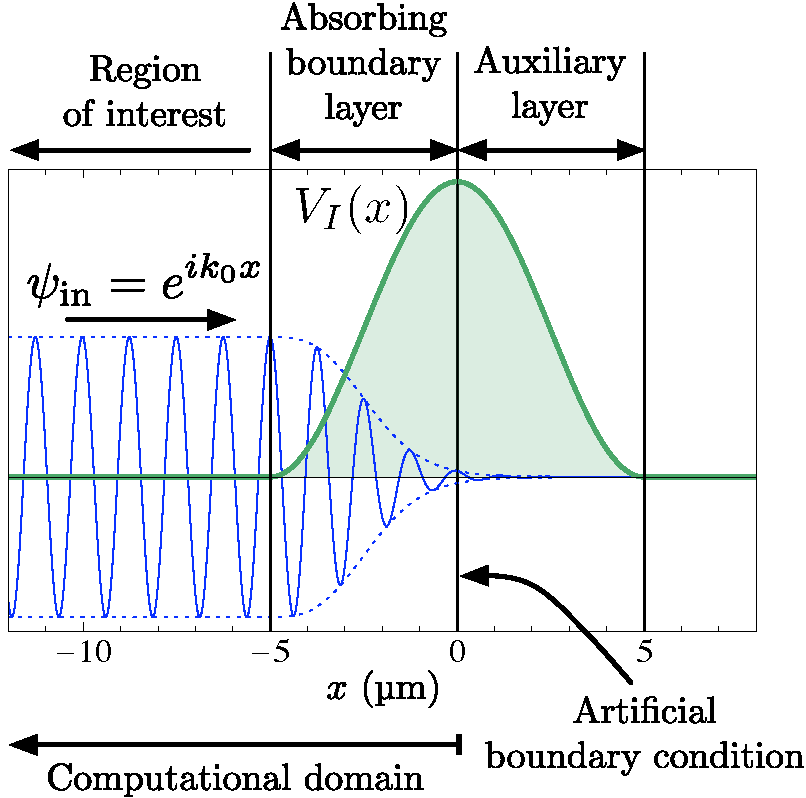
\includegraphics[width=8cm]{AbsorbingBoundaryLayerScattering}
    \caption{\label{MethodsAppendix:AbsorbingBoundaryLayerScattering} An incident wave of wavenumber $k_0$ incident on an absorbing boundary layer. The region of interest is the part of the computational domain in which the absorbing potential $V_I(x)$ is zero. An auxiliary layer is added outside of the absorbing boundary layer as a model for a number of artificial boundary conditions (see main text).}
\end{figure}

As a demonstration of the efficacy of the method described in \sectionref{Peaks:AbsorbingBoundaryTricks} for determining the rate of loss of momentum density from a region of space, we consider a wave of wavenumber $k_0$ incident from the left on an imperfect absorbing boundary layer in a 1D computational domain (see \figureref{MethodsAppendix:AbsorbingBoundaryLayerScattering}), and compare $\Phi(k, t)$ (refer to \eqref{Peaks:MomentumDensityFlux}) to the result expected in the case of a perfect absorbing boundary layer of $\displaystyle \frac{\hbar k_0}{M}\delta(k - k_0)$. In this example $s$-wave scattering will be neglected. As the computational domain in this example is effectively infinite, the wavefunction used in the evaluation of \eqref{Peaks:MomentumDensityFlux} will be restricted to be nonzero only in the absorbing boundary layer to demonstrate the finite momentum resolution obtainable from this method due to the (except in this example) finite extent of the computational domain.

As a model for a number of different artificial boundary conditions we consider there to be \emph{no} artificial boundary condition at the edge of the computational domain, and instead it to be surrounded by an `auxiliary layer' in which there is a negative imaginary potential the reflection of that in the absorbing boundary layer. The negative imaginary potential is then symmetric about the edge of the computational domain. In the case of periodic boundary conditions, the auxiliary layer will correspond to the absorbing boundary layer on the other side of the computational domain in which it is assumed that the reflected negative imaginary potential is used. In the case of Dirichlet or Neumann boundary conditions in which respectively the wavefunction or its derivative is set to zero on the boundary, the auxiliary layer corresponds to the absorbing boundary layer reflected. In either of these latter two cases, the wavefunction for the actual artificial boundary conditions will be a linear combination of the wavefunction \emph{without} the artificial boundary conditions in the absorbing boundary layer and in the auxiliary layer. Specifically, in the case of Dirichlet boundary conditions in which the wavefunction is set to zero on the boundary, the wavefunction in the presence of the artificial boundary condition $\psi_\text{abc}(\vect{x})$ will be given by $\psi_\text{abc}(\vect{x}) = \psi(\vect{x}) - \psi(-\vect{x})$ where $\psi(\vect{x})$ is the wavefunction in the absence of the artificial boundary condition, and $x=0$ corresponds to the edge of the computational domain.

To calculate $\Phi(k, t)$ from \eqref{Peaks:MomentumDensityFlux} it is necessary to know the solution $\psi(x)$ to the time-independent Schrödinger equation subject to the boundary conditions that there is an incident wave from the left with wavenumber $k_0$ and no incident wave from the right. Given two linearly independent solutions to the Schrödinger equation in the doubled absorbing boundary layer (the absorbing boundary layer / auxiliary layer region), $\psi(x)$ can be found by applying these boundary conditions. It now remains to obtain two linearly independent solutions to the time-independent Schrödinger equation within the doubled absorbing boundary layer.

Solutions to the time-independent Schrödinger equation within the doubled absorbing boundary layer can be obtained with relative ease in one dimension as it is simply an ordinary differential equation,
\begin{align}
    -\frac{\hbar^2}{2M}\frac{d^2 \psi}{dx^2} + V(x) \psi(x) &= E(k_0) \psi(x) = \frac{\hbar^2 k_0^2}{2M} \psi(x),
\end{align}
which is equivalent to
\begin{align}
    \frac{d^2 \psi}{dx^2} &= \frac{2 M}{\hbar^2} V(x) \psi(x) - k_0^2 \psi(x).
    \label{MethodsAppendix:1DTimeIndependentSchrodingerEquation}
\end{align}
Two linearly independent (but not necessarily orthogonal) solutions $\phi_1(x)$, $\phi_2(x)$ to \eqref{MethodsAppendix:1DTimeIndependentSchrodingerEquation} can be found by simply choosing two linearly independent initial conditions and numerically propagating the solutions through the potential $V(x) = -i V_I(x)$. The solution $\psi(x) = c_1 \phi_1(x) + c_2 \phi_2(x)$ can then be found by requiring continuity of the wavefunction and its derivative at the left and right edges of the doubled absorbing boundary layer,
\begin{subequations}
    \label{MethodsAppendix:1DBoundaryConditions}
    \begin{align}
        e^{i k x} + \alpha_R e^{-i k x} \Big|_\text{left} &=  c_1 \phi_1(x) + c_2 \phi_2(x) \Big|_\text{left}, \\
        \frac{d}{dx}\big( e^{i k x} + r e^{-i k x}\big) \Big|_\text{left} &=  \frac{d}{dx} \big( c_1 \phi_1(x) + c_2 \phi_2(x) \big) \Big|_\text{left},\\
        \alpha_T e^{i k x} \Big|_\text{right} &= c_1 \phi_1(x) + c_2 \phi_2(x) \Big|_\text{right}, \\
        \frac{d}{dx} \big( \alpha_T e^{i k x} \big) \Big|_\text{right} &= \frac{d}{dx} \big( c_1 \phi_1(x) + c_2 \phi_2(x) \big) \Big|_\text{right},
    \end{align}
\end{subequations}
where $\alpha_R$ and $\alpha_T$ are the reflected and transmitted amplitudes respectively. 

As a by-product of solving \eqref{MethodsAppendix:1DBoundaryConditions} for $\psi(x)$, the reflection and transmission fractions $R=\abs{\alpha_R}^2$ and $T=\abs{\alpha_T}^2$ respectively can be obtained, giving a quantitative description of the effectiveness of a given absorbing boundary layer. For reflecting artificial boundary conditions, the reflection coefficient is $R'= \abs{\alpha_R \mp \alpha_T}^2$ respectively for Dirichlet and Neumann boundary conditions, and as $\alpha_R$ and $\alpha_T$ can not both be significant simultaneously for any absorbing boundary layer that is effective over some finite range of wavenumbers, the approximation $R' \approx \max(R, T)$ can be used.  Hence $R$ and $T$ are useful measures of the effectiveness of an absorbing boundary layer independent of the artificial boundary conditions used.

\begin{figure}
    \centering
    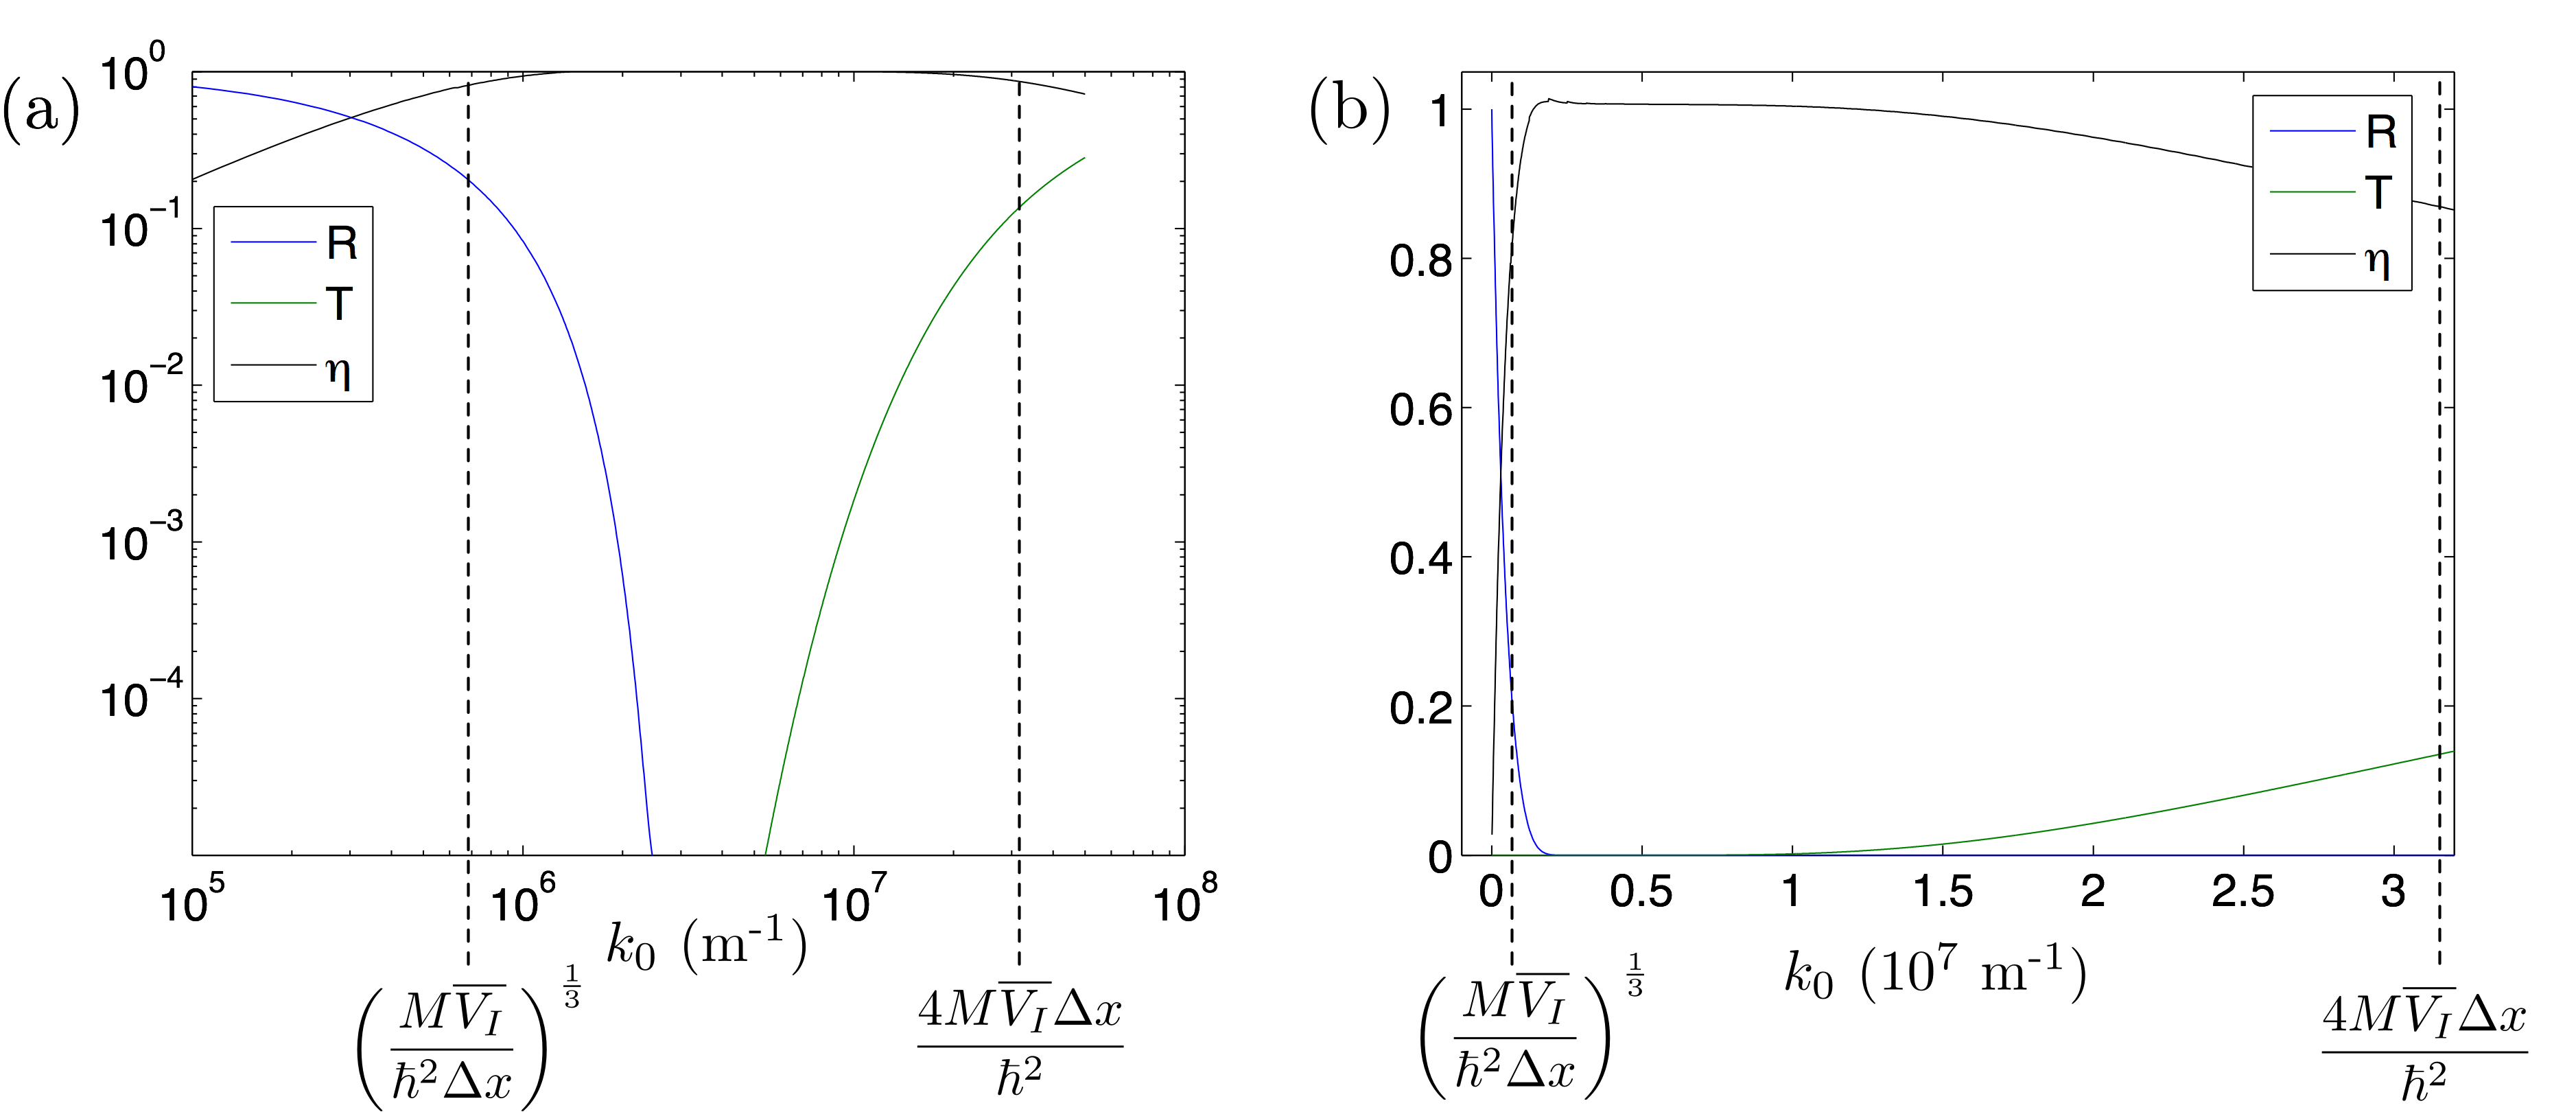
\includegraphics[width=14cm]{AbsorbingBoundaryLayerEffectiveness}
    \caption{\label{MethodsAppendix:AbsorbingBoundaryLayerEffectiveness} The reflection $R$ and transmission $T$ coefficients from a typical absorbing boundary layer as a function of wavenumber. The potential used was $\displaystyle V_I(x) = \hbar \omega \cos^2\left( \frac{\pi x}{2 \Delta x} \right)$ where $\omega = \unit[5 \times 10^4]{rad.s\textsuperscript{-1}}$ and $\Delta x = \unit[5]{\micro m}$ is the size of the absorbing boundary layer. Also marked on this figure are the approximate lower and upper bounds of the effectiveness of the absorbing boundary layer as given by \eqref{BackgroundTheory:AbsorbingBoundaryKEffectiveRange}.}
\end{figure}

In \figureref{MethodsAppendix:AbsorbingBoundaryLayerEffectiveness} the reflected and transmitted fractions $R$ and $T$ are plotted as a function of the incident wavenumber and a comparison is made to the approximate range of validity of the absorbing boundary as given by \eqref{BackgroundTheory:AbsorbingBoundaryKEffectiveRange}. 


With $\psi(x)$ determined, the steady state momentum density flux $\Phi_{k_0}(k)$ can be obtained for a given incident wavenumber $k_0$. This distribution is plotted in \figureref{MethodsAppendix:PhiAccuracy} for the same absorbing boundary used in \figureref{MethodsAppendix:PhiAccuracy}. As any real absorbing boundary layer will have finite extent, the resolution of $\Phi_{k_0}(k)$ will be limited by $\Delta k = \pi/\Delta x$, where $\Delta x$ is the width of the absorbing boundary layer. This finite resolution will prevent $\Phi_{k_0}(k)$ reproducing the exact result in the limit of a perfect absorbing boundary layer of $\displaystyle \frac{\hbar k_0}{M}\delta(k - k_0)$. As a measure of the accuracy of $\Phi_{k_0}(k)$, its integral over a range of a few $\Delta k$ should be compared to the exact answer. To this aim we define
\begin{align}
    \eta(k_0) &= \left(\frac{\hbar k_0}{M}\right)^{-1} \int_{k_0-5\Delta k}^{k_0 + 5\Delta k} dk\, \Phi_{k_0}(k),
\end{align}
where $\eta(k_0)$ is plotted in \figureref{MethodsAppendix:AbsorbingBoundaryLayerEffectiveness}. As expected, $\eta \approx 1$ over the same range of incident wavenumbers for which the absorbing boundary layer is effective.

\begin{figure}
    \centering
    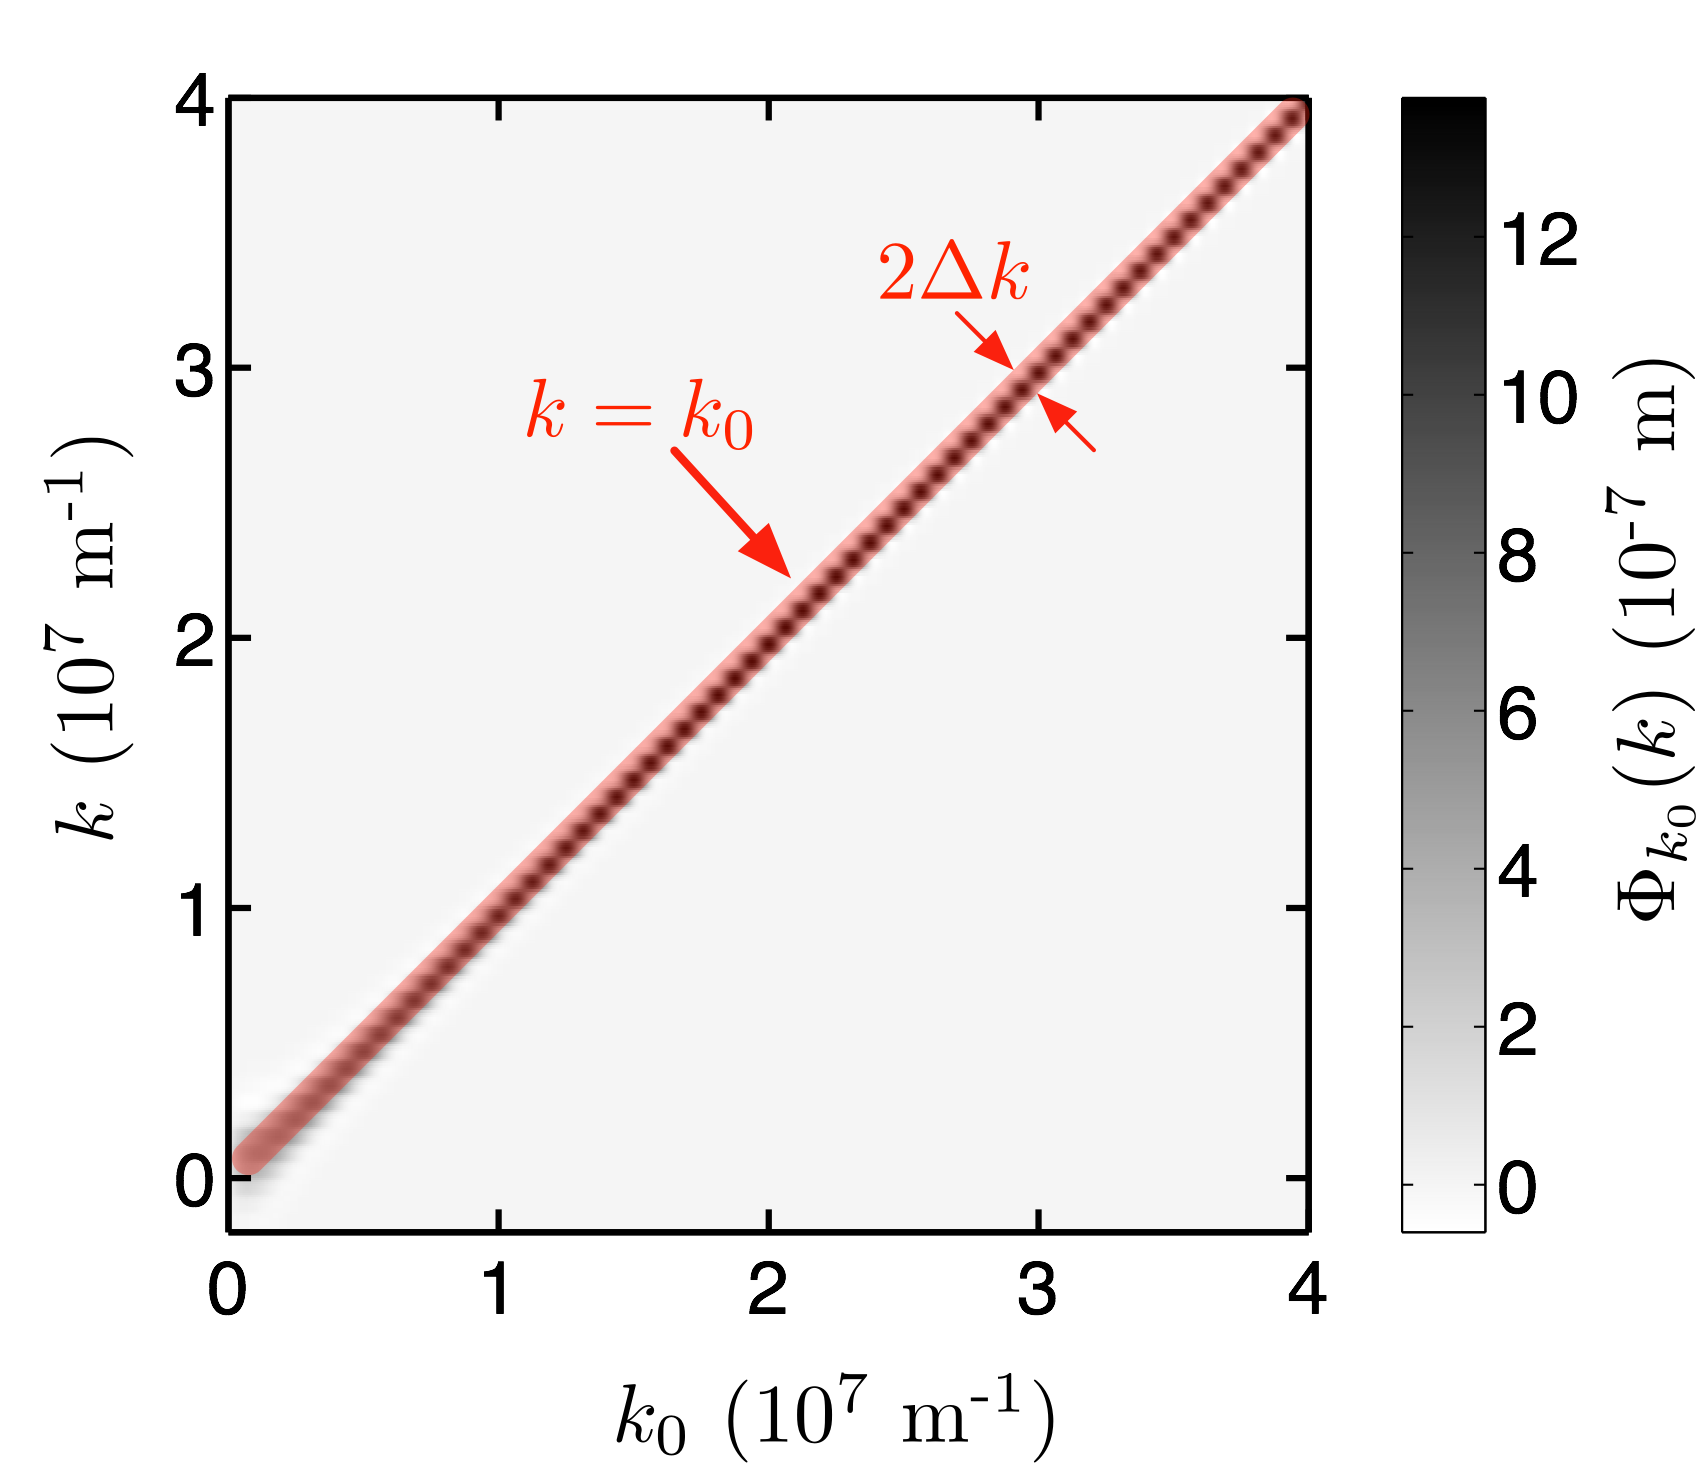
\includegraphics[width=8cm]{PhiAccuracy}
    \caption{\label{MethodsAppendix:PhiAccuracy} The momentum flux density $\Phi_{k_0}(k)$ leaving the region of interest in \figureref{MethodsAppendix:AbsorbingBoundaryLayerScattering} as a function of the incident wavenumber $k_0$. As expected, $\Phi_{k_0}(k)$ is sharply peaked around $k=k_0$. The resolution of $\Phi_{k_0}(k)$, $\Delta k$ is indicated by the width of the $k=k_0$ line.}
\end{figure}

\section[Solving the Quantum Kinetic Theory model]{Solving the Quantum Kinetic Theory model of \chapterref{KineticTheory}}
\label{MethodsAppendix:KineticTheory}

One of the difficulties involved in solving the kinetic model of \chapterref{KineticTheory} is that the energy range that the problem is defined over changes in time.  The maximum energy is simply the energy of the evaporative cut-off $\varepsilon_\text{cut}$, while the minimum energy is the chemical potential of the condensate $\mu(t)$.  A discretisation of the energy dimension over the range $[0, \varepsilon_\text{cut}]$ will suffer from problems accurately representing the lower-end of the distribution where the minimum energy of the thermal atoms is varying.  An alternative is write the problem in terms of a shifted energy coordinate $\overline{\varepsilon} \equiv \varepsilon - \mu(t)$ so that the minimum energy of the system is now fixed.  Of course the same problem now exists at the upper end of the energy range where the maximum energy $\overline{\varepsilon}_\text{max} = \varepsilon_\text{cut} - \mu(t)$ is now time-dependent.  However, at equilibrium there will be significantly fewer thermal atoms at the evaporation cut-off than there will be near the condensate (this is illustrated in \figureref{KineticTheory:EnergyDistributionFunctionEvolution}(a)).  This choice will then result in smaller numerical errors than the alternative.

Written in terms of the shifted energy variable $\overline{\varepsilon}$, the contribution due to the replenishment is
\begin{align}
    \left. \frac{\partial\big(\overline{\rho}(\overline{\varepsilon}, t) \overline{g}(\overline{\varepsilon}, t)\big)}{\partial t}\right|_\text{replenishment} &= \Gamma \overline{\rho}_0(\overline{\varepsilon}) \overline{g}_T(\overline{\varepsilon}),
    \label{MethodsAppendix:KineticTheory:ReplenishmentProcess}
\end{align}
where a bar over a function is used to indicate that it is defined in terms of the shifted energy coordinate.  The original form of this term is given by \eqref{KineticTheory:ReplenishmentProcess}.

\subsection{Density of states}
\label{MethodsAppendix:QKTDensityOfStates}

Although the evolution equations for the kinetic model \eqref{KineticTheory:EvolutionEquations} are written in terms of the product of the density of states $\rho(\varepsilon, t)$ and the energy distribution function $g(\varepsilon, t)$, it will be necessary to separately determine the energy distribution function to evaluate the collisional contributions given in the following section. To extract the energy distribution function it is necessary to have an explicit expression for the density of states for the thermal cloud. This density of states is not simply the same as that for a harmonic trap as the thermal modes will experience a mean-field repulsion due to the condensate mode. The effective potential experienced by the thermal atoms is
\begin{align}
    V_\text{eff}(\vect{r}, t) &= V_\text{trap}(\vect{r}) + 2 g n_c(\vect{r}, t), \label{MethodsAppendix:QKTEffectivePotential}
\end{align}
where $V_\text{trap}(\vect{r})$ is the potential due to the magnetic trap, $g = 4\pi \hbar^2 a/m$, $a$ is the \emph{s}-wave scattering length and $n_c(\vect{r}, t)$ is the condensate density which was assumed to follow a Thomas-Fermi distribution in \chapterref{KineticTheory}.  Note that the `2' in the above expression is the full Hartree-Fock mean field experienced by the thermal atoms (see \eqref{Peaks:ThermalParticleEnergySpectrum}, or~\citep[Chapter 8]{PethickSmith} for further details) which is twice the mean-field repulsion experienced by condensate atoms.  This is essentially due to the thermal atoms being distinguishable from the condensate atoms, while the condensate atoms are indistinguishable from one another.

The density of states in the presence of the effective potential \eqref{MethodsAppendix:QKTEffectivePotential} is given by
\begin{align}
    \rho(\varepsilon, t) &= \int \frac{d \vect{r}\, d \vect{p}}{(2\pi \hbar)^3} \,\delta\left(\varepsilon - V_\text{eff}(\vect{r}, t) - \vect{p}^2/2 m\right).
    \label{MethodsAppendix:DensityOfStatesDefinition}
\end{align}
The integrals are performed in~\citep{Bijlsma:2000} giving the following result in terms of the shifted energy coordinate (Eqs.~49 and 50 in~\citep{Bijlsma:2000})
\begin{align}
    \overline{\rho}(\overline{\varepsilon}, t) &= \frac{2}{\pi \hbar \overline{\omega}} \left[I_-(\overline{\varepsilon}) + I_+(\overline{\varepsilon})\right],
\end{align}
where the functions $I_\pm(\overline{\varepsilon})$ are
\begin{align}
    I_-(\overline{\varepsilon}) &= \left.\frac{u_-^3 x}{4} - \frac{a_- u_- x}{8} - \frac{a_-^2}{8}\ln(x + u_-)\right|_{x=\sqrt{\max\{0, -a_-\}}}^{x=\sqrt{2\mu/\hbar \overline{\omega}}}, \label{MethodsAppendix:QKTIMinus}\\
    I_+(\overline{\varepsilon}) &= \left.- \frac{u_+^3 x}{4} + \frac{a_+ u_+ x}{8} + \frac{a_+^2}{8} \arcsin\left(\frac{x}{\sqrt{a_+}}\right)\right|_{x=\sqrt{2\mu/\hbar\overline{\omega}}}^{x=\sqrt{a_+}}, \label{MethodsAppendix:QKTIPlus}
\end{align}
with $a_\pm = 2(\overline{\varepsilon}\pm \mu)/\hbar\overline{\omega}$, and $u_\pm = \sqrt{a_\pm \mp x^2}$. Note that there is a minor typo in~\citet{Bijlsma:2000}, the lower limit of $I_-(\overline{\varepsilon})$ is given as $x=\sqrt{\max\{0, a_-\}}$, while it should read $x=\sqrt{\max\{0, -a_-\}}$ as in \eqref{MethodsAppendix:QKTIMinus}.

\subsection{Collision and energy-redistribution in Quantum Kinetic Theory}
\label{MethodsAppendix:QKTOtherTerms}

The forms of the collision and energy-redistribution terms of the kinetic model described in \chapterref{KineticTheory} were omitted there for sake of clarity as their derivation was not part of the work presented there.  A full derivation of these terms is given in~\citep{Bijlsma:2000,Proukakis:2008}.

The contribution due to thermal--thermal collisions is given in Eq.~26 of~\citep{Bijlsma:2000} and has the form
\begin{align}
    \begin{split}
        \left. \frac{\partial\big(\overline{\rho}(\overline{\varepsilon}_1, t) \overline{g}(\overline{\varepsilon}_1, t)\big)}{\partial t}\right|_\text{thermal--thermal} &= \frac{m^3 g^2}{2 \pi^3 \hbar^7} \int d\overline{\varepsilon}_2 \int d\overline{\varepsilon}_3 \int d\overline{\varepsilon}_4 \,\overline{\rho}(\overline{\varepsilon}_\text{min}, t)\\
        &\relphantom{=} \times\delta(\overline{\varepsilon}_1 + \overline{\varepsilon}_2 - \overline{\varepsilon}_3 - \overline{\varepsilon}_4) \\
        &\relphantom{=} \times [ (1+\overline{g}_1) (1+\overline{g}_2) \overline{g}_3 \overline{g}_4 - \overline{g}_1 \overline{g}_2 (1+\overline{g}_3) (1+\overline{g}_4)],
    \end{split}
\end{align}
where $\overline{\varepsilon}_\text{min}$ is the minimum of the $\overline{\varepsilon}_i$, and $\overline{g}_i = \overline{g}(\overline{\varepsilon}_i, t)$. 

The contribution due to thermal--condensate collisions is given by Eq.~53 and Eq.~58--60 of~\citep{Bijlsma:2000} and has the form
\begin{align}
    \begin{split}
        \left. \frac{\partial\big(\overline{\rho}(\overline{\varepsilon}_1, t) \overline{g}(\overline{\varepsilon}_1, t)\big)}{\partial t}\right|_\text{thermal--condensate} &= \frac{m^3 g^2}{2 \pi^3 \hbar^7} \int d \overline{\varepsilon}_2 \int d\overline{\varepsilon}_3 \int d\overline{\varepsilon}_4 \,\delta(\overline{\varepsilon}_2 - \overline{\varepsilon}_3 - \overline{\varepsilon}_4)\\
        &\relphantom{=}\times\left[ \delta(\overline{\varepsilon}_1 - \overline{\varepsilon}_2) - \delta(\overline{\varepsilon}_1 - \overline{\varepsilon}_3) - \delta(\overline{\varepsilon}_1- \overline{\varepsilon}_4)\right]\\
        &\relphantom{=} \times \left[(1+\overline{g}_2)\overline{g}_3 \overline{g}_4 - \overline{g}_2 (1+\overline{g}_3)(1+\overline{g}_4) \right]\\
        &\relphantom{=}\times  \int_{\overline{U}_\text{eff}(\vect{r}, t) \leq \overline{U}_-} d \vect{r}\, n_c(\vect{r}, t),
    \end{split}
    \label{MethodsAppendix:QKTRhoGThermalCondensateEvolution}
\end{align}
where $\displaystyle \overline{U}_- = \frac{2}{3}\left[(\overline{\varepsilon}_3 + \overline{\varepsilon}_4)-\sqrt{\overline{\varepsilon}_3^2 - \overline{\varepsilon}_3 \overline{\varepsilon}_4 + \overline{\varepsilon}_4^2}\right]$, and $\overline{U}_\text{eff}(\vect{r}, t) = U_\text{eff}(\vect{r}, t) - \mu(t)$.
The corresponding contribution to the evolution of the condensate number is simply
\begin{align}
    \left. \frac{d N_0}{d t}\right|_\text{thermal--condensate} &= - \int d\overline{\varepsilon} \,\left. \frac{\partial\big(\overline{\rho}(\overline{\varepsilon}, t) \overline{g}(\overline{\varepsilon}, t)\big)}{\partial t}\right|_\text{thermal--condensate}.
    \label{MethodsAppendix:QKTNThermalCondensateEvolution}
\end{align}


Finally, the contribution due to energy redistribution is (Eqs.~32 and 52 in~\citep{Bijlsma:2000})
\begin{align}
    \left. \frac{\partial\big(\overline{\rho}(\overline{\varepsilon}_1, t) \overline{g}(\overline{\varepsilon}_1, t)\big)}{\partial t}\right|_\text{redistribution} &= - \frac{\partial \big( \overline{\rho}_\text{w} \overline{g}\big)}{\partial \overline{\varepsilon}},
    \label{MethodsAppendix:QKTRedistributionEvolution}
\end{align}
where $\overline{\rho}_\text{w}$ is the weighted density of states
\begin{align}
    \overline{\rho}_\text{w}(\overline{\varepsilon}) &= \frac{2}{\pi \hbar \overline{\omega}} \left[ I_-(\overline{\varepsilon}) - I_+(\overline{\varepsilon})\right] \frac{d \mu}{dt},
\end{align}
where the functions $I_\pm(\overline{\varepsilon})$ are given in \eqref{MethodsAppendix:QKTIMinus} and \eqref{MethodsAppendix:QKTIPlus}.


\subsection{Three-body loss in Quantum Kinetic Theory}
\label{MethodsAppendix:QKT3BodyLoss}

The dominant density-dependent loss process in Bose-Einstein condensates is three-body loss~\citep{Burt:1997fk,Soding:1999}. In \chapterref{KineticTheory} it was argued that three-body loss was an important process in the operation of the pumped atom laser scheme proposed there.  The following derivation of the three-body loss contribution to the kinetic model \eqref{KineticTheory:EvolutionEquations} was performed by \emph{Matthew Davis} and is presented for completeness.

Three-body loss (or three-body recombination) is the process in which three atoms collide forming a bound dimer with the third necessary to ensure both energy and momentum conservation.  The binding energy is sufficient to give the products of a three-body recombination process sufficient kinetic energy to rapidly escape the trap.  Three-body loss is then well-described by the master equation term
\begin{align}
    \left. \frac{d \hat{\rho}}{d t}\right|_\text{3-body loss} &= \frac{1}{3}L_3 \int d \vect{x} \,\mathcal{D} \left[ \hat{\Psi}^3(\vect{x}) \right] \hat{\rho},
    \label{MethodsAppendix:ThreeBodyLossMasterEquationTerm}
\end{align}
where $\mathcal{D}[\hat{c}]\hat{\rho} = \hat{c}\hat{\rho} \hat{c}^\dagger - \frac{1}{2}(\hat{c}^\dagger \hat{c}\hat{\rho} + \hat{\rho} \hat{c}^\dagger \hat{c})$ is the usual decoherence superoperator, and $L_3 = \unit[5.8\times 10^{-30}]{cm\textsuperscript{6}s\textsuperscript{-1}}$~\citep{Burt:1997fk} is the three-body recombination loss rate constant.  This equation, first derived by~\citep{Jack:2002} has the familiar form of a decoherence superoperator with the state undergoing loss as the argument (cf. \sectionref{PenningIonisationAppendix:MasterEquation}). %This is a reasonable approximation as three-body recombination couples the state $\hat{\Psi}^3$ to a state that is rapidly depopulated.

The loss rate of atoms from the system due to three-body loss is readily obtained from \eqref{MethodsAppendix:ThreeBodyLossMasterEquationTerm} as
\begin{align}
    \left.\frac{d N}{dt} \right|_\text{3-body loss} &=  \Tr\left\{\int d \vect{r}\,\hat{\Psi}^\dagger(\vect{r})\hat{\Psi}(\vect{r}) \left.\frac{d \hat{\rho}}{dt}\right|_\text{3-body loss} \right\} = - L_3 \int d \vect{r}\, \mean{\hat{\Psi}^\dagger(\vect{r})^3 \hat{\Psi}(\vect{r})^3}.
    \label{MethodsAppendix:ThreeBodyLossNumberLossRate}
\end{align}

To separate the contributions to \eqref{MethodsAppendix:ThreeBodyLossNumberLossRate} due to the thermal and condensed components, we use an approach similar to that of the Bogoliubov theory discussed in \sectionref{Peaks:ElementaryExcitations}.  We write the annihilation operator $\hat{\Psi}$ in terms of its mean value $\Psi \equiv \mean{\hat{\Psi}}$ and the deviation operator $\delta \hat{\Psi} \equiv \hat{\Psi} - \Psi$ and substitute this into \eqref{MethodsAppendix:ThreeBodyLossNumberLossRate}.  In contrast to \sectionref{Peaks:ElementaryExcitations} in which the zero-temperature limit was considered, the deviation operator defined here represents thermal fluctuations, which cannot be considered to be small.  Higher powers of $\delta\hat{\Psi}$ can therefore not be neglected.  However, thermal fluctuations have no well-defined phase relationship to one another or to the condensate.  Expectation values containing an unequal number of creation and annihilation deviation operators such as $\mean{\delta\hat{\Psi}\delta\hat{\Psi}}$ can therefore be assumed to be zero (cf. \eqref{Peaks:HamiltonianPowerSeriesQuadraticTerm} in which the $\delta\hat{\Psi}^\dagger \delta\hat{\Psi}^\dagger$ and $\delta\hat{\Psi}\delta\hat{\Psi}$ terms were retained as there is a well-defined phase relationship between the quasiparticles and the condensate).

Performing the substitution described, \eqref{MethodsAppendix:ThreeBodyLossNumberLossRate} becomes
\begin{align}
    \begin{split}
        \left.\frac{d N}{dt} \right|_\text{3-body loss} &=  -L_3 \int d \vect{r}\, \Big\{[n_c(\vect{r})]^3 + 9 [n_c(\vect{r})]^2 \mean{\delta\hat{\Psi}^\dagger(\vect{r}) \delta\hat{\Psi}(\vect{r})}\\
        &\relphantom{=-L_3 \int d \vect{r}\,\Big\{} + 9 n_c(\vect{r}) \mean{\delta\hat{\Psi}^\dagger(\vect{r})^2 \delta\hat{\Psi}(\vect{r})^2} + \mean{\delta\hat{\Psi}^\dagger(\vect{r})^3 \delta\hat{\Psi}(\vect{r})^3}\Big\},
    \end{split}
    \label{MethodsAppendix:ThreeBodyLossNumberLossRateInTermsOfDeviationOperators}
\end{align}
where $n_c(\vect{r}) = \abs{\Psi(\vect{r})}^2$ is the condensate density.

The non-condensate density is given by $n_T(\vect{r}) = \mean{\delta\hat{\Psi}^\dagger(\vect{r}) \delta\hat{\Psi}(\vect{r})}$.  As thermal states are Gaussian, the higher-order expectation values in the previous expression may be simplified by the application of Wick's theorem~\citep{Wick:1950} giving
\begin{align}
    \mean{\delta\hat{\Psi}^\dagger(\vect{r})^2 \delta\hat{\Psi}(\vect{r})^2} &= 2 [n_T(\vect{r})]^2, \\
    \mean{\delta\hat{\Psi}^\dagger(\vect{r})^3 \delta\hat{\Psi}(\vect{r})^3} &= 6 [n_T(\vect{r})]^3.
\end{align}
Substituting these expressions back into \eqref{MethodsAppendix:ThreeBodyLossNumberLossRateInTermsOfDeviationOperators} yields
\begin{align}
    \left.\frac{d N}{dt} \right|_\text{3-body loss} &=  -L_3 \int d \vect{r}\, [n_c(\vect{r})]^3 + 9 [n_c(\vect{r})]^2 n_T(\vect{r}) + 18 n_c(\vect{r}) [n_T(\vect{r})]^2 + 6 [n_T(\vect{r})]^3.
    \label{MethodsAppendix:ThreeBodyLossNumberLossRateInTermsOfDensities}
\end{align}

The evaluation of this loss rate requires the evaluation of the condensate and thermal densities.  The condensate density $n_c(\vect{r})$ is fully determined by the condensate occupation $N_0(t)$ within the Thomas-Fermi approximation that has already been made elsewhere in the derivation of the kinetic model.  The first term of \eqref{MethodsAppendix:ThreeBodyLossNumberLossRateInTermsOfDensities} only involves the condensate density and may be evaluated analytically
\begin{align}
    \frac{d N_0}{dt} &= - L_3 \frac{15^{4/5}}{168 \pi^2} \left(\frac{m \overline{\omega}}{\hbar \sqrt{a}} \right)^{12/5} N_0^{9/5}.
\end{align}
The remaining terms of \eqref{MethodsAppendix:ThreeBodyLossNumberLossRateInTermsOfDensities} require an expression for the thermal density $n_T(\vect{r})$, which can be obtained from the energy distribution function $g(\varepsilon)$ and the density of states $\rho(\varepsilon)$.

The total number of thermal atoms $N_T$ can be written as
\begin{align}
    N_T &= \int d\varepsilon\, \rho(\varepsilon) g(\varepsilon),
    \label{MethodsAppendix:NThermalDefinition}
\end{align}
where the density of states is defined by \eqref{MethodsAppendix:DensityOfStatesDefinition}.  Substituting this into \eqref{MethodsAppendix:NThermalDefinition} and rearranging the order of integrals gives
\begin{align}
    N_T &= \int d \vect{r}\, \int d\varepsilon\, \rho(\varepsilon, \vect{r}) g(\varepsilon),
    \label{MethodsAppendix:NThermalInTermsOfRhoER}
\end{align}
where we have defined
\begin{align}
    \rho(\varepsilon, \vect{r}) &= \int d \vect{p}\, \delta\left(\varepsilon - V_\text{eff}(\vect{r}, t) - \vect{p}^2/2m\right) = \frac{m^{3/2}}{\sqrt{2} \pi^2 \hbar^3} \sqrt{\varepsilon - V_\text{eff}(\vect{r})}.
\end{align}
The thermal density can be identified from \eqref{MethodsAppendix:NThermalInTermsOfRhoER}
\begin{align}
    n_T(\vect{r}) &= \int d\varepsilon\, \rho(\varepsilon, \vect{r}) g(\varepsilon).
    \label{MethodsAppendix:nThermalInTermsOfRhoER}
\end{align}

The remaining terms of \eqref{MethodsAppendix:ThreeBodyLossNumberLossRateInTermsOfDensities} can now be expressed in terms of the energy distribution function $g(\varepsilon)$ and the density of states $\rho(\varepsilon)$ by substituting \eqref{MethodsAppendix:nThermalInTermsOfRhoER} for one of the factors of $n_T(\vect{r})$ in each term
\begin{align}
    -L_3 \int d \vect{r}\, 9 [n_c(\vect{r})]^2 n_T(\vect{r}) &= - L_3 \int d\varepsilon\, g(\varepsilon) \int d \vect{r}\, 9 \rho(\varepsilon, \vect{r}) [n_c(\vect{r})]^2, \label{MethodsAppendix:Condensate2Thermal1}\\
    -L_3 \int d \vect{r}\, 18 n_c(\vect{r}) [n_T(\vect{r})]^2 &= - L_3 \int d\varepsilon\, g(\varepsilon) \int d \vect{r}\, 18 \rho(\varepsilon, \vect{r}) n_c(\vect{r}) n_T(\vect{r}), \label{MethodsAppendix:Condensate1Thermal2}\\
    -L_3 \int d \vect{r}\, 6 [n_T(\vect{r})]^3 &= - L_3 \int d\varepsilon\, g(\varepsilon) \int d \vect{r}\, 6 \rho(\varepsilon, \vect{r}) [n_T(\vect{r})]^2. \label{MethodsAppendix:Condensate0Thermal3}
\end{align}
From these expressions the rate of loss of atoms of energy $\varepsilon$ from the distribution can be identified
\begin{align}
    \left.\frac{\partial\big(\rho(\varepsilon) g(\varepsilon)\big)}{\partial t}\right|_\text{3-body loss} &= -L_3 \int d \vect{r}\, \rho(\varepsilon, \vect{r}) g(\varepsilon) \left\{ 3 [n_c(\vect{r})]^2 + 12 n_c(\vect{r}) n_T(\vect{r}) + 6 [n_T(\vect{r})]^2 \right\},
    \label{MethodsAppendix:QKT3BodyLossDistributionEvolution}
\end{align}
where the contributions due to the terms involving only one or two thermal atoms have been multiplied by $1/3$ and $2/3$ respectively to share appropriately the total loss.  The corresponding term for the condensate number evolution is
\begin{align}
    \begin{split}
        \left. \frac{d N_0}{dt} \right|_\text{3-body loss} &= - L_3 \frac{15^{4/5}}{168 \pi^2} \left(\frac{m \overline{\omega}}{\hbar \sqrt{a}} \right)^{12/5} N_0^{9/5}\\
        &\relphantom{=} - L_3 \int d\varepsilon \int d \vect{r}\, \rho(\varepsilon, \vect{r}) g(\varepsilon) \left\{6 [n_c(\vect{r})]^2 + 6 n_c(\vect{r}) n_T(\vect{r}) \right\},
    \end{split}
    \label{MethodsAppendix:QKT3BodyLossCondensateEvolution}
\end{align}
where the contributions due to the terms involving only one or two condensate atoms have been multiplied by $1/3$ and $2/3$ respectively.

% The value of the three-body loss rate constant used in \chapterref{KineticTheory} was that obtained by~\citet{Burt:1997fk} of $L_3 = \unit[5.8\times 10^{-30}]{cm\textsuperscript{6}s\textsuperscript{-1}}$ (denoted $K_3^{c}$ in that work).



%%%%%%%%%%%%%%%%%%%%%%%%%%%%%%%%%%%%%%%%%%%%%%%%%%%%%%%%%%%%%%%%%%%%%%%%%%%%%%%%%%%%%%%%%%%%%%%%%%%%%%%%%%%%%%

% \section{Convolutions}
% Unrelated to thesis but important: When doing convolutions you must truncate the range of the interaction potential to prevent interacting with the `copies' of the density that you do want to interact with. This Fourier transform \emph{must} be calculated analytically. The range of the grid must also be such that the density is nonzero within a rectangular prism with side lengths $\frac{1}{2}$ that of the computational domain. This is to prevent the left part of the density interacting with the right part due to the wrap-around~\citep{Ronen:2006}.
% \begin{align}
%     \mathcal{F}(f * g) &= \sqrt{2 \pi} \mathcal{F}(f) \mathcal{F}(g)
% \end{align}

\chapter{Calculational tools}
\label{ToolsAppendix}
\graphicspath{{Figures/ToolsAppendix/}{Figures/Common/}}

This is an appendix in which we \emph{briefly} (hah!) summarise the features and methods of \texttt{xpdeint} with particular attention paid to those features used in this thesis.

\begin{itemize}
    \item Spectral method
    \item IP operator
    \item Various basis functions
    \item Coupled ODE-PDE systems
    \item Gaussian quadrature
    \item Stochastic integration
    \item Distributed simulations
    \item Cross-propagation
\end{itemize}

\bibliography{thesis}


\end{document}
